\frontmatter

\begin{acknowledgments}

Tôi xin được gửi lời cảm ơn sâu sắc đến PGS.TS Quản Thành Thơ -
giảng viên giám sát và hướng dẫn trực tiếp quá trình thực hiện
đề tài này. Nhờ có những chỉ dẫn, góp ý tận tình của thầy mà
tôi có thể hoàn thành được tốt Luận văn tốt nghiệp này.

Tôi chân thành cám ơn quý thầy, cô trong khoa Khoa Học Và Kỹ Thuật
Máy Tính, trường Đại học Bách Khoa - ĐHQG - HCM đã tận tình
truyền đạt kiến thức trong những năm chúng tôi học tập ở trường.
Với vốn kiến thức tích lũy được trong suốt quá trình học tập là
nền tảng cho quá trình nghiên cứu.

Cuối cùng, tôi xin chúc quý thầy, cô dồi dào sức khỏe và thành công
trong sự nghiệp cao quý.

\end{acknowledgments}

\begin{abstractTV}

Hỗ trợ tư vấn khách hàng là một trong những khía cạnh chính của
trải nghiệm người dùng đối với các dịch vụ trực tuyến. Tuy nhiên,
với sự gia tăng của các kỹ thuật xử lý ngôn ngữ tự nhiên, ngành
công nghiệp đang xem xét giải pháp hệ thống đối thoại tự động
(Chatbot) để cung cấp dịch vụ chất lượng cho người dùng. Trong
luận án này, tôi trình bày nghiên cứu, xây dựng một hệ thống
Chatbot như vậy.

Đầu tiên, phần giới thiệu về thị trường tư vấn khách hàng trực tuyến
được trình bày cũng như đánh giá nhanh về lĩnh vực hội thoại tự động.
Ngoài ra, còn trình bày về mục tiêu và giới hạn của đề tài. Sau đó,
trình bày các công trình nghiên cứu khoa học trước đây và hiện tại
được sử dụng để phát triển Chatbot.

Phần tiếp theo là trình bày các lý thuyết đằng sau các kỹ thuật được
sử dụng. Chủ yếu là kỹ thuật học tăng cường, mô hình học tăng cường
cho một Chatbot hướng mục tiêu được thảo luận.

Sau đó, một kiến trúc phần mềm có thể mở rộng cho Chatbot được đề xuất
và giải thích, quá trình huấn luyện mô hình cũng được mô tả.
Các công nghệ sử dụng được liệt kê và trình bày cách
hiện thực hệ thống rõ ràng.

Phần còn lại của luận văn tập trung vào việc đánh giá mô hình, một loạt
các trường hợp thử nghiệm thực tế được đưa ra và chúng cho thấy rằng
hành vi của Chatbot là khả quan. Ngoài ra, việc kiểm thử hệ thống
cũng được trình bày để đảm bảo hệ thống làm việc ổn định.

Cuối cùng, tóm tắt những kết quả đạt được, thảo luận những vấn đề mà
mô hình còn gặp phải, và đề xuất hướng phát triển tiếp theo của
đề tài trong tương lai.

\end{abstractTV}

\begin{abstractTA}

Customer support is perhaps one of the key aspects of the user
experience for online services. However, with the proliferation
of natural language processing techniques, the industry is
looking at automated dialogue system (Chatbot) solutions to provide
quality service to users. In this thesis, I present research, build
such a chatbot system.

First, an introduction to the online client consulting market is
presented as well as a quick review of the automated conversation
field. In addition, the objectives and limitations of the thesis
are also presented. Then, present the previous and
current scientific works used to develop chatbots.

The following section delves into the theoretical underpinnings of
the techniques employed, with a primary focus on reinforcement
learning models for goal-oriented chatbots.

Afterwards, a scalable software architecture for the chatbot is
proposed and explained, the model training process is also described.
The technologies used are listed and the system implementation is
clearly presented.

The rest of the thesis focuses on the model evaluation, a series of
real test cases are given and they show that the chatbot's behavior
is positive. In addition, system testing is also presented to
ensure the system works stably.

Finally, summarize the results achieved, discuss the problems that
the model still faces, and propose the next direction of the topic
in the future.

\end{abstractTA}

\begin{declaration}

Tôi xin cam đoan đây là công trình nghiên cứu của riêng tôi dưới
sự giám sát và hướng dẫn của PGS.TS Quản Thành Thơ. Việc lựa chọn
và thực hiện đề tài xuất phát từ nhu cầu thực tiễn cũng như
nguyện vọng của bản thân. Nội dung nghiên cứu và các kết quả
đều là trung thực và chưa từng được công bố trước đây. Các số liệu
được sử dụng cho quá trình phân tích, nhận xét được chính tôi
thu thập từ nhiều nguồn khác nhau và sẽ được ghi rõ
trong phần tài liệu tham khảo.

Ngoài ra, tôi cũng có sử dụng một số nhận xét, đánh giá và số liệu
của các tác giả khác, cơ quan tổ chức khác. Tất cả đều có trích dẫn
và chú thích nguồn gốc.

Nếu phát hiện có bất kì sự gian lận nào, tôi xin hoàn toàn chịu
trách nhiệm về nội dung Luận văn của mình. Trường Đại học Bách Khoa
- ĐHQG - HCM không liên quan đến những vi phạm tác quyền, bản quyền
do tôi gây ra trong quá trình thực hiện.

\begin{flushright}
\begin{minipage}{8cm} % hoặc điều chỉnh 5.5cm, 7cm tùy ý
\centering
TP. Hồ Chí Minh, ngày .... tháng .... năm ........

Sinh viên thực hiện \\[2cm]
\thesisstudent
\end{minipage}
\end{flushright}

\end{declaration}

\tableofcontents
\listoftables
\listoffigures

\mainmatter

\chapter {Giới thiệu}

\section{Giới thiệu đề tài}
Khách hàng là nguồn sống của bất cứ cửa hàng, doanh nghiệp nào.
Chính vì thế, chăm sóc khách hàng (CSKH) trở thành một trong những
yếu tố sống còn và đòi hỏi rất nhiều đầu tư về công sức và tiền bạc.
Có nhiều hình thức khác nhau để chăm sóc khách hàng như qua email,
qua điện thoại, qua các diễn đàn trực tuyến, và qua tin nhắn
trực tuyến.

Ở nước ta, việc giải đáp thắc mắc của khách hàng qua tin nhắn
trực tuyến đang được ưa chuộng. Tuy nhiên, việc này còn thực hiện
một cách thủ công và gặp nhiều khó khăn như: tốn rất nhiều
thời gian và chi phí chi trả cho nhân viên chỉ để trả lời những
câu hỏi đơn giản và giống nhau. Chính vì vậy, nhu cầu cấp thiết
là cần một hệ thống điều khiển thông minh, tự động để mang lại
hiệu quả cao hơn và Chatbot là một sự lựa chọn hoàn hảo. Cụ thể,
tác dụng của Chatbot trong lĩnh vực chăm sóc khách hàng như sau:

\begin{itemize}
    \item Đưa thông tin chính xác tới từng tệp khách hàng.
    \item Trả lời tự động mọi câu hỏi của khách hàng đưa ra
    mọi lúc mọi nơi.
    \item Tăng sự tương tác của khách hàng và doanh nghiệp.
    \item Tự động chăm sóc khách hàng thường xuyên 24/7.
    \item Giảm chi phí đầu tư.
\end{itemize}

Chatbot chăm sóc khách hàng phù hợp với nhiều loại mô hình
doanh nghiệp từ kinh doanh online (cung cấp thông tin sản phẩm,
đưa ra các thông tin gợi ý, v.v.), hay là các nhà hàng, rạp
chiếu phim (cung cấp các tùy chọn menu, chọn vị trí chổ ngồi,
thanh toán, v.v.), và cũng được sử dụng nhiều trong lĩnh vực
y tế, chăm sóc sức khoẻ.

Hiện nay, có rất nhiều hướng tiếp cận để xây dựng một Chatbot,
tùy vào mục đích sử dụng. Trong đó, một phương pháp Chatbot khá
phổ biến dựa trên quy tắc (rule-based), nó được huấn luyện bằng
một hệ thống phân cấp các quy tắc được xác định trước, chuyển đổi
các hành động của người dùng là đầu vào thành các hành động đầu ra
của Chatbot. Vì vậy, với hệ thống này nó không thể phản hồi với
các mẫu đầu vào hay các từ khóa không phù hợp với các quy tắc
hiện có. Và với mỗi mẫu đầu vào, nó sẽ có một quy tắc phản hồi
cố định, các quy tắc này giúp cho hệ thống làm việc được chặt chẽ.
Tuy nhiên, các hành vi sẽ bị lặp đi lặp lại, dẫn tới một hệ thống
cứng nhắc và nhàm chán. Một phương pháp khác, hiện thực một hệ thống
hội thoại tự do hơn như \textit{Sequence To Sequence}. Nó huấn luyện
để cho tác nhân tự tạo ra các câu trả lời và có khả năng xử lý được
các câu mà nó chưa từng gặp. Tuy nhiên, nó không theo dõi được và
hướng hội thoại theo cùng một ngữ cảnh. Trong luận án này, đề tài
hướng đến một phương pháp mới, hiện đại, và phát triển ngày càng
mạnh mẽ hiện nay, là phương pháp học tăng cường (reinforcement learning).
Phương pháp này nó mô hình hóa cho tác nhân nên thực hiện các hành động
sao cho tối ưu hóa phần thưởng tích lũy. Vì thế, sau quá trình huấn luyện,
các tác nhân nó vẫn theo được các quy tắc ban đầu đặt ra, hướng hội thoại
vào cùng một ngữ cảnh. Và tùy vào trạng thái hiện tại của hội thoại,
tác nhân phản hồi linh hoạt hơn, có khả năng vượt ra ngoài quy tắc
ban đầu được xây dựng.

\section{Mục tiêu và các giai đoạn thực hiện của đề tài}
\label{sec:muctieu}
Trong phạm vi nghiên cứu của đề tài này, tập trung xây dựng một
hệ thống hội thoại tự động có thể tư vấn cho khách hàng thông tin
về các sản phẩm thời trang như quần áo, váy đầm, v.v. Cụ thể,
hệ thống bao gồm các tính năng sau:

\begin{itemize}
    \item Cung cấp nguồn dữ liệu tin cậy để Chatbot có thể tư vấn
    đầy đủ và chính xác cho người dùng.
    \item Hiểu được ý định, nhu cầu của người dùng khi họ tham gia
    hội thoại với Chatbot, trích xuất được các thông tin mà người dùng
    cung cấp để truy vấn chính xác, thoả mãn yêu cầu của người dùng.
    \item Thỏa mãn, hoàn thành được yêu cầu của người dùng khi
    tham gia cuộc hội thoại. Mang lại sự hài lòng tốt nhất
    có thể cho người dùng.
    \item Giao tiếp với người dùng một cách linh hoạt, bám sát với
    luồng hội thoại để mang lại trải nghiệm tốt nhất
    có thể cho người dùng.
\end{itemize}

Để có thể đạt được những tính năng trên, cần xác định một số công việc
phải giải quyết như sau:

\begin{itemize}
    \item Tìm kiếm và thu thập dữ liệu phù hợp với nội dung đề tài.
    Lọc nhiễu, trích xuất các thông tin cần thiết để lưu trữ vào
    cơ sở dữ liệu phục vụ cho nhu cầu truy vấn cho Chatbot.
    \item Khảo sát nhu cầu của người dùng khi cần được tư vấn
    thông tin sản phẩm, từ đó xây dựng được các kịch bản
    tư vấn cho người dùng.
    \item Huấn luyện cho hệ thống, sử dụng mô hình học tăng cường,
    để có thể đưa ra quyết định cho mỗi hành động khi giao tiếp
    với người dùng một cách tốt nhất.
    \item Xây dựng các hệ thống đi kèm khác để hỗ trợ cho việc
    giao tiếp với người dùng như truy vấn dữ liệu chính xác,
    trả về đúng thông tin người dùng mong muốn.
    \item Xây dựng bộ sinh câu phản hồi của Chatbot với ngôn từ
    tự nhiên tạo cảm giác thoải mái cho người dùng.
    \item Xây dựng với bộ giao diện ứng dụng thân thiện, dễ sử dụng.
\end{itemize}

\section{Các giai đoạn thực hiện}
Với những mục tiêu đã đề ra ở mục \ref{sec:muctieu}, đề tài được
thực hiện qua các giai đoạn như sau:

\begin{itemize}
    \item \textbf{Giai đoạn 1:} Tìm kiếm và thu thập các thông tin về
    sản phẩm thời trang để thiết kế ra các hoạt động mà Chatbot
    có thể hỗ trợ.
    \item \textbf{Giai đoạn 2:} Khảo sát và thu thập các thông tin từ
    người dùng để thiết kế ra các ý định của người dùng.
    \item \textbf{Giai đoạn 3:} Thiết kế hệ thống và định nghĩa cách
    kiểm thử, đánh giá hệ thống.
    \item \textbf{Giai đoạn 4:} Xây dựng mô hình huấn luyện gồm các
    bộ sinh phản hồi, bộ quản lý hội thoại, bộ mô phỏng người dùng và lỗi.
    \item \textbf{Giai đoạn 6:} Xây dựng các thành phần cấu thành
    ứng dụng Chatbot đơn giản. Đồng thời, tổng hợp các thành phần
    còn lại thành một hệ thống hoàn chỉnh.
    \item \textbf{Giai đoạn 7:} Tiến hành kiểm thử và đánh giá hệ thống.
\end{itemize}

\section{Giới hạn của đề tài}
\label{sec:scope}
Các nhu cầu của khách hàng trong lĩnh vực tư vấn thời trang là rất
phong phú nên việc đáp ứng hết tất cả nhu cầu là rất khó khăn.
Vì vậy, trong đề tài này tôi sẽ cố gắng đáp ứng được những
nhu cầu đã được định nghĩa.

Trong đề tài này, chỉ tập trung vào việc nghiên cứu và sử dụng mô hình
học tăng cường huấn luyện cho Chatbot để mang lại độ chính xác lẫn
tự nhiên có thể chấp nhận được, mang lại trải nghiệm thoải mái
cho người dùng.

Đồng thời, xây dựng bộ mô phỏng người dùng và tạo lỗi để tự động
sinh ra các mẫu hội thoại có tính tự nhiên và dùng nó để huấn luyện
cho Chatbot.

Ngoài ra, đề tài còn xây dựng ứng dụng Chatbot với giao diện đơn giản
có thể giao tiếp với người dùng dễ dàng.

\section{Cấu trúc luận văn}

\begin{itemize}
    \item \textbf{Chương 1:} Giới thiệu tổng quan về đề tài, mục tiêu,
    giới hạn và các giai đoạn thực hiện đề tài.
    \item \textbf{Chương 2:} Trình bày một số công trình có liên quan
    tới đề tài.
    \item \textbf{Chương 3:} Trình bày các kiến thức nền tảng có
    liên quan tới đề tài. Và cách hoạt động của nó trên bài toán
    của đề tài.
    \item \textbf{Chương 4:} Trình bày phương pháp giải quyết
    bài toán: mô tả về kiến trúc hệ thống, quá trình huấn luyện
    mô hình học tăng cường.
    \item \textbf{Chương 5:} Trình bày các công cụ và công nghệ
    sử dụng để giải quyết bài toán.
    \item \textbf{Chương 6:} Trình bày cách thức hiện thực hệ thống.
    \item \textbf{Chương 7:} Trình bày cách thức kiểm thử và
    đánh giá hệ thống.
    \item \textbf{Chương 8:} Tổng kết quá trình thực hiện luận văn,
    những hạn chế và hướng phát triển.
\end{itemize}

\chapter{Các công trình liên quan}

\section{Các công trình nghiên cứu liên quan đến Chatbot hỗ trợ
thương mại điện tử}

\subsection{Bài báo về Chatbot hỗ trợ y tế tự động}
Đây là bài báo có tên \textit{Automated Medical Chatbot}
\cite{automatedmedical}. Trong bài báo này, tác giả đề xuất một
hệ thống có khả năng đặt ra nhiều câu hỏi cho người dùng cho đến khi
xác định được căn bệnh mà người dùng đang gặp phải. Đây gần như là
một hệ thống tư vấn y tế. Hệ thống sẽ thu thập các thông tin từ
người dùng như triệu chứng, sau đó đưa ra những căn bệnh mà
người dùng có thể mắc phải và hỏi người dùng về cảm giác của họ.
Sau khi nhận được nhiều dữ liệu, nó sẽ tìm ra căn bệnh
có khả năng xảy ra nhất.

Ngoài ra, họ đặt ra một khái niệm mức ngưỡng giúp phát hiện mức độ
của vấn đề. Tuỳ vào mức độ nghiêm trọng của bệnh mà nó sẽ đề xuất
các biện pháp khắc phục và thuốc cho người dùng hoặc kết nối
người dùng với bác sĩ.

Trong bài báo, tác giả đã sử dụng phương pháp AIML (Artificial
Intelligence Mark-up Lang\-uage) để hiểu được các mẫu (pattern)
trong tin nhắn của người dùng thông qua các thẻ (tag)
được xác định trước.

Ví dụ, ta có một số các \textit{pattern tag} được xác định
trước như ví dụ \ref{exam:pattern}. Khi người dùng nói
\enquote{I am suffering from headache.} (Tôi đang bị đau đầu),
hệ thống sẽ ánh xạ tin nhắn của người dùng với các pattern
và phát hiện trùng với pattern \enquote{I am suffering from *},
\enquote{headache}
(đau đầu) sẽ được thay thế bởi dấu *. Sau đó hệ thống sẽ truy cập
vào cơ sở dữ liệu với thông tin đầu tiên là triệu chứng đau đầu
và đưa ra hành động tiếp theo.

\renewcommand{\textboxenvname}{Ví dụ}
\begin{textbox}[exam:pattern]{Một số các pattern tag}
\begin{Verbatim}[breaklines=true, breakanywhere=true]
<pattern>I am feeling like *</pattern>
<pattern>I am having *</pattern>
<pattern>I am suffering from *</pattern>
\end{Verbatim}
\end{textbox}

Cùng với một số các thành phần khác thì hệ thống của họ đưa ra có thể
tư vấn khách hàng như ví dụ \ref{exam:medicaldialog}. Đầu tiên có thể
thực hiện với câu chào hỏi, và hỏi về vấn đề của người dùng. Sau khi
nhận được thông tin về triệu chứng là đau đầu, Chatbot sẽ hỏi thêm các
thông tin triệu chứng khác để làm rõ căn bệnh. Cuối cùng sau khi lấy
đủ thông tin, Chatbot đưa ra kết luận về căn bệnh người dùng mắc phải
và cách chữa trị.

\renewcommand{\textboxenvname}{Ví dụ}
\begin{textbox}[exam:medicaldialog]{Một mẫu hội thoại của Chatbot}
\begin{Verbatim}[breaklines=true, breakanywhere=true]
User: Hello
Chatbot: Hi there, tell me how can I help you?
User: I am having an Headache
Chatbot: Are you having pain in your eyes?
User: Yes
Chatbot: Do you feel like vomiting?
User: yes I do
Chatbot: I think you are most likely having a migraine attack
Chatbot: Taking "ibuprofen" 2 tablets would reduce pain in you eyes. Also take "aspirin" 20ml to help you tackle vomiting. Do take a nap and dont forget to wash your eyes with luke warm water. Avoid using digital screen until you feel better.
\end{Verbatim}
\end{textbox}

\subsection{Bài báo về Chatbot hỗ trợ mua sắm trực tuyến}
Đây là bài báo có tên \textit{SuperAgent: A Customer Service Chatbot
for E-commerce Websites} \cite{superagent}. Trong bài báo này, họ
giới thiệu SuperAgent, một Chatbot dịch vụ khách hàng, sử dụng dữ liệu
thương mại điện tử quy mô lớn và công khai. SuperAgent tận dụng dữ liệu
từ mô tả sản phẩm trong trang cũng như nội dung do người dùng tạo từ
các trang web thương mại điện tử. Ngoài ra, SuperAgent sinh câu phản hồi
dựa trên bốn mô hình chạy song song, bao gồm các bộ câu hỏi và trả lời
(QA) thực tế, bộ tìm kiếm QA thường gặp, bộ QA văn bản định hướng ý kiến,
và mô hình cuộc trò chuyện chit-chat.

\begin{figure}[ht]
    \centering
    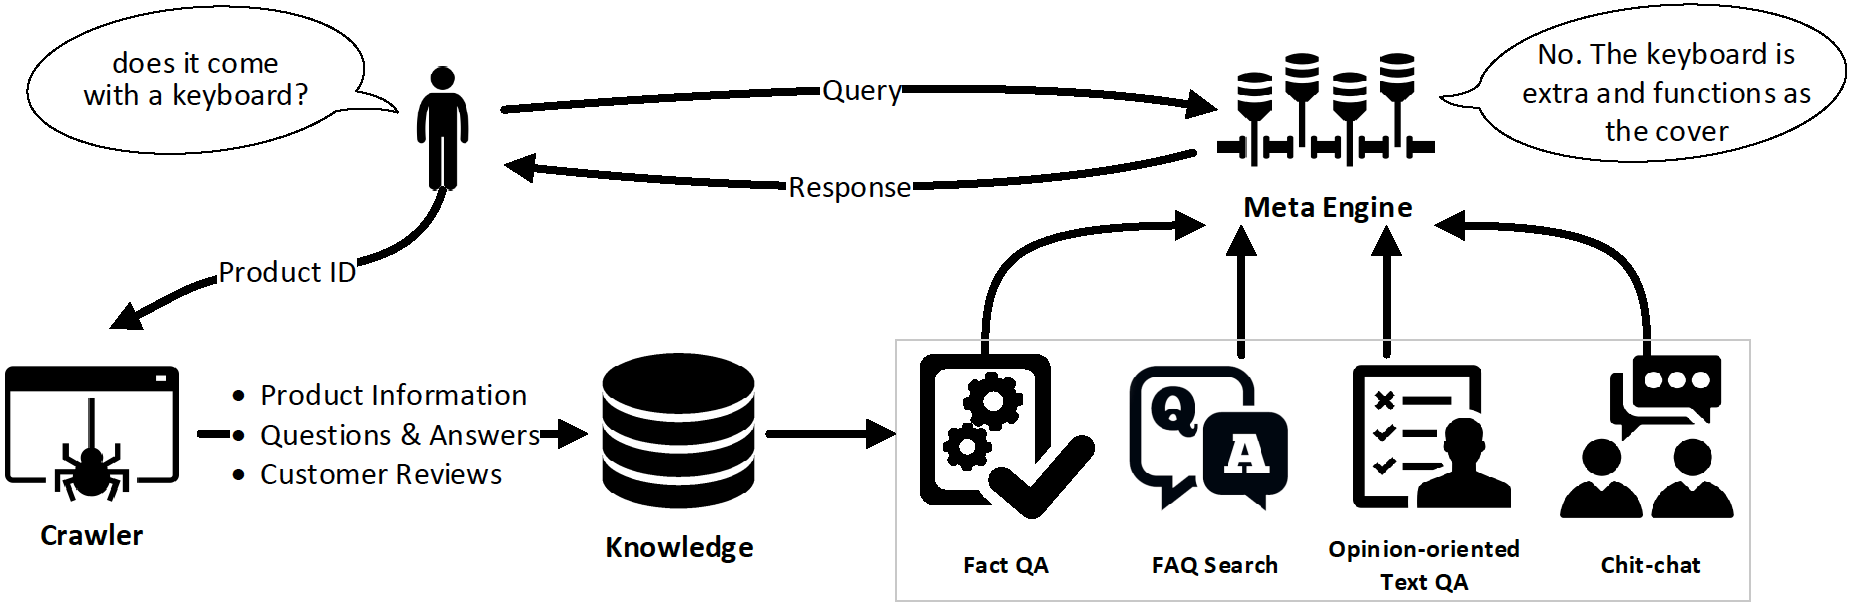
\includegraphics[width=1\textwidth]{thesis/chatbot/congtrinh/img/superagent.png}
    \caption{Kiến trúc tổng quát của hệ thống SuperAgent}
    \label{fig:superagent}
\end{figure}

Hình \ref{fig:superagent} mô tả tổng quan hệ thống của SuperAgent.
Như hình cho thấy, khi trang sản phẩm được truy cập lần đầu tiên,
SuperAgent thu thập các dữ liệu thông tin sản phẩm (PI), bộ câu hỏi
và trả lời (QA) và phản hồi của khách hàng (CR) từ trang web. Ưu điểm
của mẫu thiết kế này là họ không cần triển khai trình thu thập
thông tin cho các trang web. Thay vào đó, khi người dùng truy cập
trang, SuperAgent sẽ được thông báo vì có tiện ích bổ sung được
liên kết với mỗi trang web. Do đó, SuperAgent mang lại rất ít lượt
tải web bổ sung cho các trang web đã được lưu trữ. Bên cạnh đó,
kiến trúc này giúp cho việc cập nhật dữ liệu rất dễ thực hiện,
trong đó các trang được truy cập thường xuyên sẽ được cập nhật
thường xuyên và ngược lại. Với một truy vấn đầu vào từ khách hàng,
các công cụ khác nhau sẽ được xử lý song song. Nếu một trong ba câu
trả lời từ ba công cụ đầu tiên có độ tin cậy cao, thì chatbot sẽ
trả về câu trả lời từ phản hồi. Nếu không, công cụ trò chuyện sẽ
tạo ra một câu trả lời từ các nhóm câu trả lời được phép xác định
trước.

\begin{figure}[ht]
    \centering
    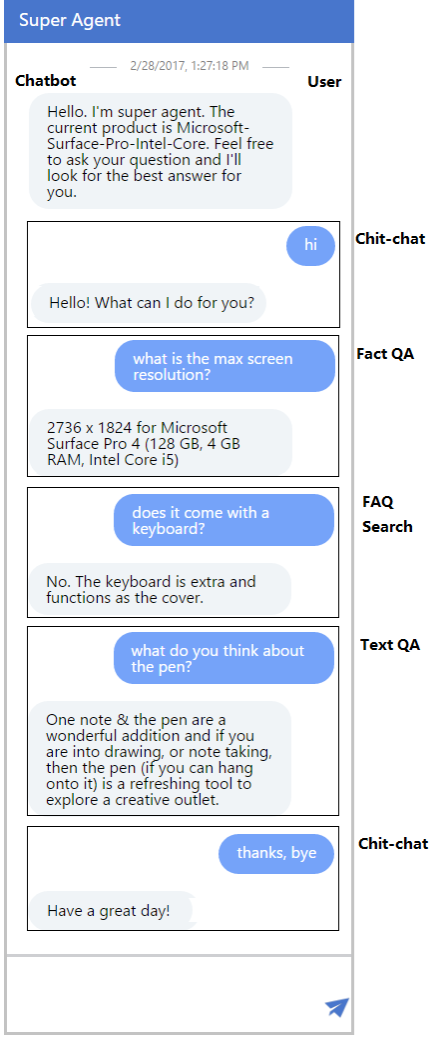
\includegraphics[width=0.45\textwidth]{thesis/chatbot/congtrinh/img/superagentdialog.png}
    \caption{Một mẫu hội thoại của SuperAgent}
    \label{fig:superagentdialog}
\end{figure}

Hình \ref{fig:superagentdialog} cho thấy một tình huống điển hình
khi một khách hàng yêu cầu SuperAgent giúp đỡ. Khi khách hàng mở
cửa sổ trò chuyện trong trình duyệt web, SuperAgent đầu tiên sẽ
phát hiện sản phẩm nào đang được truy cập. Sau đó, SuperAgent tự
giới thiệu và xác nhận rằng khách hàng đang ghé thăm sản phẩm.
Khách hàng có thể chào hỏi SuperAgent hoặc hỏi các câu hỏi cụ thể.
Như hình \ref{fig:superagentdialog} cho thấy, SuperAgent có thể
trả lời các câu hỏi sự thật (Fact QA) bằng cách sử dụng thông tin
sản phẩm trong trang, thực hiện tìm kiếm câu hỏi thường gặp (FAQ
Search) từ các cặp QA của khách hàng, lấy câu trả lời QA từ đánh giá
của khách hàng và cuối cùng là chào hỏi khách hàng bằng cách sử dụng
công cụ trò chuyện chit-chat. Các hộp thoại được điều phối bởi
công cụ meta để các truy vấn khác nhau chuyển đến các công cụ
tương ứng. Vì các trang web thương mại điện tử được cập nhật
thường xuyên và nội dung mới do người dùng tạo liên tục xuất hiện,
SuperAgent cũng cập nhật dữ liệu và mô hình định kỳ theo tần suất
truy cập của khách hàng.

\subsection{Bài báo về Chatbot hỗ trợ sân bay}
Đây là bài báo có tên \textit{Design and implementation of an airport
chatbot} \cite{airport}. Trong bài báo này, họ mô tả động lực và
quá trình phát triển của một Chatbot nhằm cung cấp thông tin và hỗ trợ
cho khách du lịch trực tiếp bên trong nhà ga Sân bay Venice hoặc bằng
các giao diện gián tiếp, chẳng hạn như ứng dụng di động hoặc trang web.

Để phát triển Chatbot, họ quyết định dựa trên một nền tảng được
cung cấp bởi một công ty công nghệ lớn: Microsoft Azure Bot Service.
Tất cả các dịch vụ cloud và dịch vụ máy chủ cho trang web và quản lý
email đều đã được Microsoft quản lý. Họ sử dụng bộ xử lý ngôn ngữ
tự nhiên để hiểu loại (ý định) và các tham số (thực thể) của câu hỏi
mà người dùng có thể hỏi, bất kể nó được hỏi như thế nào.

Ví dụ, trong Chatbot của họ, câu \enquote{what is the weather like in
Venice?} (Thời tiết ở Venice như thế nào?) được chuyển thành một
đối tượng như ví dụ \ref{exam:airport}, có thể được thao tác bởi
Chatbot.

\renewcommand{\textboxenvname}{Ví dụ}
\begin{textbox}[exam:airport]{Biểu diễn của một câu hỏi}
\begin{Verbatim}[breaklines=true, breakanywhere=true]
{
    intent : "weather",
    parameters : {
        address : {
            city : "Venice"
        },
        date-time : "2019-01-20T12:00:00+02:00"
    }
}
\end{Verbatim}
\end{textbox}

Hệ thống họ phát triển có các chức năng sau:

\begin{itemize}
    \item Câu hỏi thường gặp (FAQ).
    \item Các câu hỏi chung về sân bay do tổng đài thu thập.
    \item Thông tin chuyến bay.
    \item Thông tin giao thông địa phương đến và đi từ sân bay
    (kế hoạch chuyến đi).
    \item Vị trí của các cửa hàng, hoạt động hoặc cổng bên trong
    sân bay.
    \item Thông tin về bãi đậu xe.
    \item Tìm hành lý thất lạc.
    \item Tìm đồ bị mất.
\end{itemize}

Sơ đồ chung của Chatbot được thể hiện trong hình \ref{fig:airportarch}.
LUIS là dịch vụ xử lý như NLP. Nó có giao diện web cho phép tạo ra các
ý định và thực thể nhưng không cung cấp phản hồi trực tiếp. Tích hợp
LUIS cho phép bot hiểu ngôn ngữ tự nhiên, phát hiện lỗi chính tả,
sử dụng nhận dạng giọng nói và nhận ra mục đích của người dùng. QnA
Maker là một dịch vụ API dựa trên đám mây tạo ra một lớp câu hỏi và
câu trả lời tương tự như một cuộc trò chuyện dữ liệu. Các câu hỏi và
câu trả lời được nhập từ nội dung bán cấu trúc (semi-structure),
chẳng hạn như tài liệu thường gặp, các đường dẫn và hướng dẫn sử dụng
sản phẩm. Chatbot phải giao tiếp với các dịch vụ cơ sở dữ liệu và API
của sân bay để trả lời các câu hỏi cụ thể liên quan đến sân bay.

Các câu hỏi của người dùng được quản lý và phân tích bởi bộ điều phối
(dispatcher) để quyết định xem câu hỏi có yêu cầu phản hồi linh động
hay không, nếu có nó phải được gửi đến LUIS, hoặc câu hỏi tĩnh được
gửi đến bộ tạo câu hỏi và trả lời (QnA). Quyền truy cập vào cơ sở
hạ tầng sân bay nội bộ và các lệnh gọi API bên ngoài được thực hiện
trực tiếp bởi dịch vụ bot Azure.

\begin{figure}[ht]
    \centering
    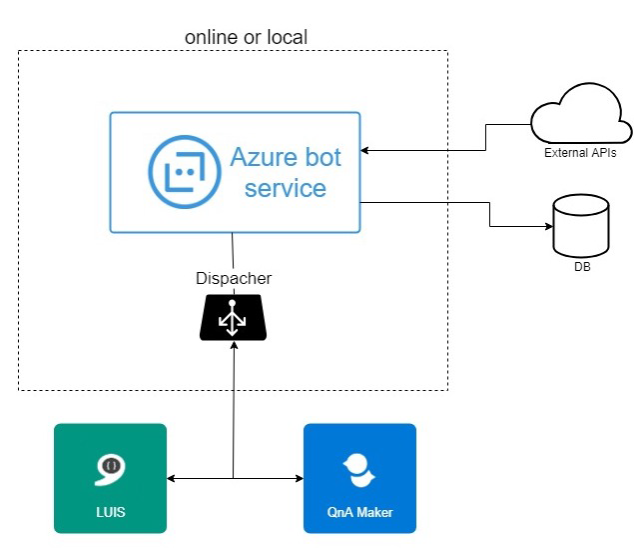
\includegraphics[width=0.8\textwidth]{thesis/chatbot/congtrinh/img/airportarch.png}
    \caption{Sơ đồ tổng quát của Chatbot sân bay}
    \label{fig:airportarch}
\end{figure}

\subsection{Bài báo về Chatbot hỗ trợ dịch vụ cung ứng}
Đây là bài báo có tên \textit{E-commerce Distributed Chatbot System}
\cite{commerce}. Trong bài báo này, họ trình bày một hệ thống Chatbot
phân tán cho chuỗi cung ứng. Hệ thống của họ bao gồm một số dịch vụ:
dịch vụ trò chuyện, dịch vụ bot, dịch vụ xử lý ngôn ngữ tự nhiên và
dịch vụ chuỗi cung ứng. Nó sử dụng giao tiếp WebSocket giữa giao diện
người dùng và bot, phân tích truy vấn của người dùng và cung cấp
thông tin về các đơn đặt hàng và nguồn cung cấp đã được truy vấn.

Kiến trúc hệ thống của Chatbot phân tán cho chuỗi cung ứng được
đề xuất trong bài báo như trên hình \ref{fig:commerce}.

\begin{figure}[ht]
    \centering
    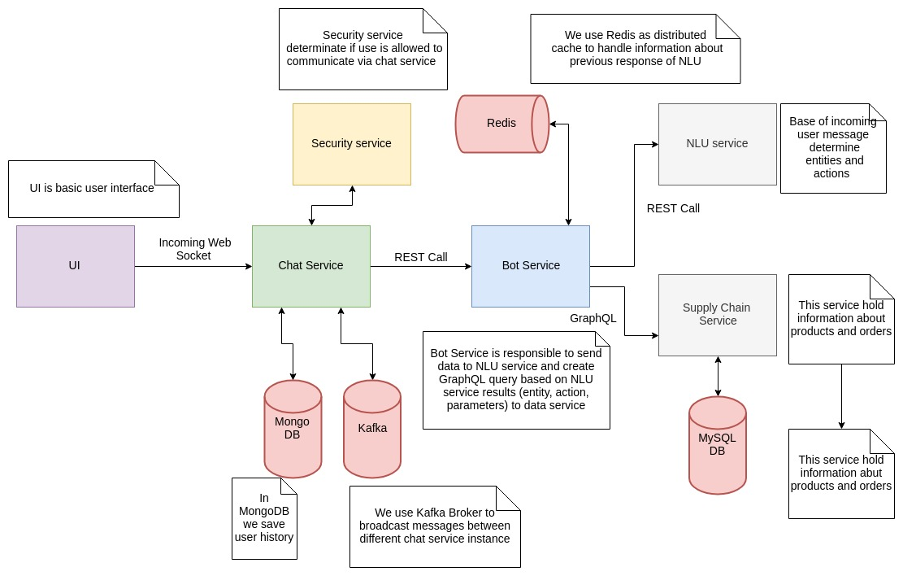
\includegraphics[width=1\textwidth]{thesis/chatbot/congtrinh/img/commerce.png}
    \caption{Kiến trúc hệ thống Chatbot phân tán}
    \label{fig:commerce}
\end{figure}

Hệ thống bao gồm năm dịch vụ con:
\begin{itemize}
    \item Dịch vụ trò chuyện (Chat Service): chịu trách nhiệm về
    giao tiếp WebSocket giữa giao diện người dùng và bot.
    \item Dịch vụ bot (Bot Service): phân tích thông điệp của
    người dùng, xây dựng yêu cầu truy xuất thông tin cần thiết
    và cung cấp cho người dùng một cách dễ hiểu.
    \item Dịch vụ hiểu ngôn ngữ tự nhiên (NLU Service): phân tích
    thông điệp của người dùng, trích xuất thông tin về ý định của
    người dùng và các đối tượng làm phong phú thêm thông tin về
    ý định đó.
    \item Dịch vụ chuỗi cung ứng (Supply Chain Service): chứa
    thông tin về đơn đặt hàng và nguồn cung cấp cho người dùng.
    \item Dịch vụ an ninh (Security Service): chịu trách nhiệm
    về bảo mật thông tin liên lạc qua dịch vụ trò chuyện.
\end{itemize}

Sơ đồ triển khai của hệ thống Chatbot phân tán cho chuỗi cung ứng
dựa trên kiến trúc đề xuất được hiển thị trên hình
\ref{fig:commercediagram}.
Hệ thống được triển khai dưới dạng có tám bộ chứa docker.

\begin{figure}[ht]
    \centering
    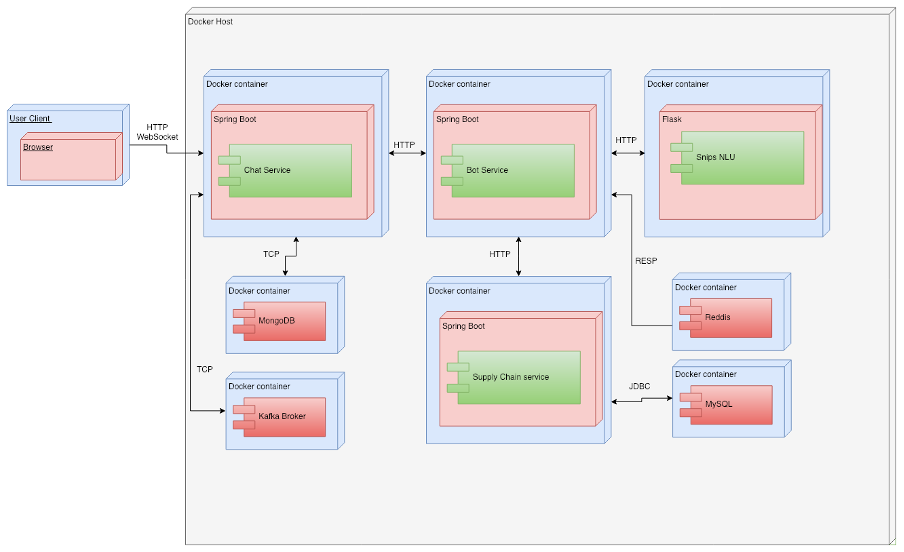
\includegraphics[width=1\textwidth]{thesis/chatbot/congtrinh/img/commerce_diagram.png}
    \caption{Sơ đồ triển khai của hệ thống Chatbot phân tán}
    \label{fig:commercediagram}
\end{figure}

Đánh giá thử nghiệm của họ đối với hệ thống Chatbot phân tán cho
chuỗi cung ứng được dựa trên hai nhóm mẫu thử nghiệm: mẫu thử nghiệm
tuân theo mẫu dữ liệu đào tạo và mẫu thử nghiệm sử dụng nhiều từ
đồng nghĩa trong truy vấn của người dùng dựa trên ngôn ngữ tự nhiên.

Kết quả thử nghiệm của họ cho thấy khả năng nhận dạng đúng trong 90\%
các câu người dùng thử nghiệm mẫu và tỷ lệ nhận dạng 65\% đối với các
truy vấn của người dùng với các từ đồng nghĩa của các câu đó.

Chất lượng nhận dạng dịch vụ của NLU được tăng thêm lên 83\% đối với
các truy vấn của người dùng khác với các mẫu tham chiếu, bằng cách
đào tạo bổ sung hệ thống NLU với dữ liệu thử nghiệm không được
giải quyết đúng cách.

Ngoài ra, họ còn đánh giá hiệu suất của nó bằng cách sử dụng thử nghiệm
áp lực (stress test) thông qua Gatling. Kết quả thử nghiệm cho thấy rằng
hệ thống có thể xử lý tới 10000 phiên người dùng mà không cần mở rộng
bất kỳ máy chủ nào trong 60 phút. Độ trễ chính của hệ thống đến từ
việc không thể triển khai nhiều kết nối WebSocket cùng một lúc.

\section{Các công trình nghiên cứu liên quan đến Chatbot sử dụng
mô hình học tăng cường}

\subsection{Bài báo về Chatbot sử dụng hành động phân cụm và phần thưởng}
Đây là bài báo có tên \textit{Deep Reinforcement Learning for
Chatbots Using Clustered Actions and Human-Likeness Rewards}
\cite{clustered}. Trong bài báo này, sử dụng các hành động phân cụm
thay vì lượng lớn các hành động và một bộ khen thưởng đơn giản
dựa trên cách cho điểm giống con người thu được từ dữ liệu hội thoại
giữa con người với con người.

Họ huấn luyện các tác nhân học tăng cường sâu (DRL) bằng cách sử dụng
dữ liệu trò chuyện trong văn bản thô - mà không có bất kỳ chú thích
thủ công nào.

Kịch bản học tập của họ như sau:

\begin{itemize}
    \item Lấy một tập dữ liệu về các cuộc hội thoại giữa con người
    với con người ở dạng văn bản thô, tác nhân sẽ đóng vai trò của
    một trong hai người trong cuộc hội thoại, để học cách chọn những
    câu giống người khi tiếp xúc với cả những câu giống người và
    không giống người.
    \item Các tương tác của môi trường-tác nhân bao gồm cả các
    tương tác dữ liệu-tác nhân - không có trình mô phỏng người dùng
    như trong các hệ thống hội thoại hướng tác vụ.
    \item Trong mỗi lượt hội thoại, tác nhân quan sát trạng thái của
    môi trường thông qua mạng nơ-ron học sâu. Mạng này nó mô hình hóa
    một biểu diễn của tất cả các câu được nêu ra trong cuộc hội thoại
    cùng với một tập hợp các câu trả lời của ứng viên hoặc hành động
    của tác nhân (các hành động được phân cụm theo phương pháp của họ).
    \item Sau đó tác nhân chọn một hành động, biểu diễn dựa trên mức
    từ của hành động được gửi đến môi trường.
    \item Tác nhân nhận được lịch sử hội thoại đã được cập nhật và
    phần thưởng cho hành động đó, cho đến khi đáp ứng điều kiện chấm dứt.
\end{itemize}

Quá trình này, được minh họa trong hình \ref{fig:clusterarch} - được
thực hiện lặp đi lặp lại cho đến khi kết thúc một cuộc hội thoại cho
nhiều cuộc hội thoại nếu cần, tức là cho đến khi không có cải thiện
nào nữa về hiệu suất của tác nhân.

\begin{figure}[ht]
    \centering
    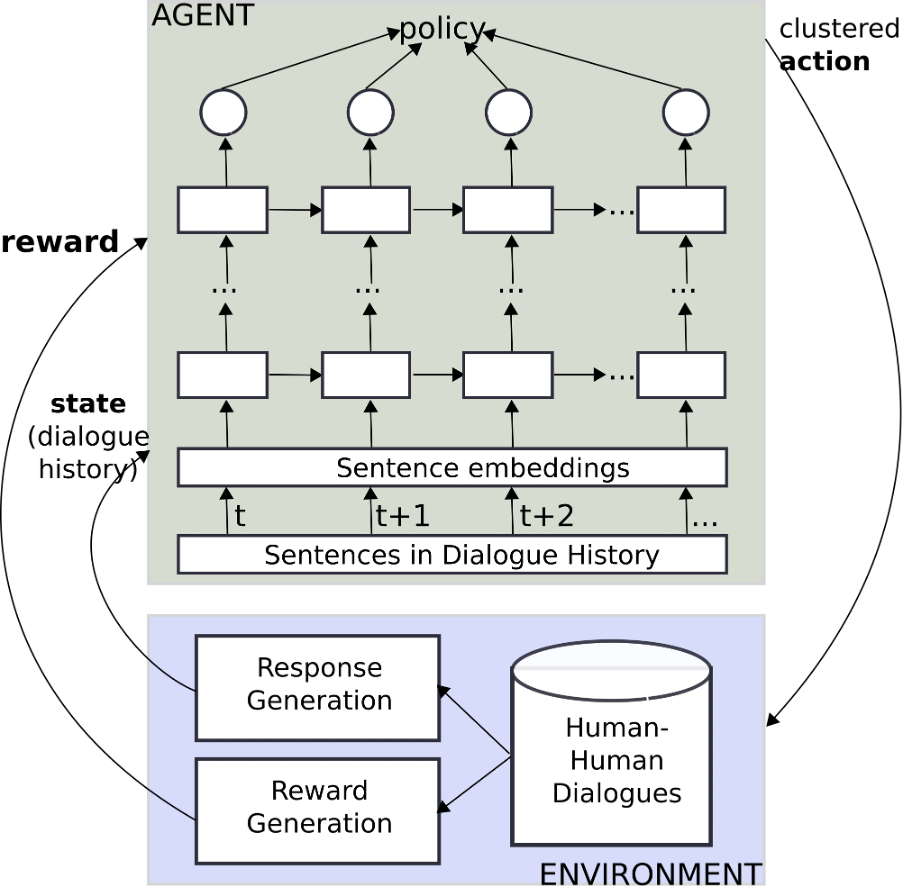
\includegraphics[width=0.8\textwidth]{thesis/chatbot/congtrinh/img/clusterarch.png}
    \caption{Kiến trúc hệ thống Chatbot DRL}
    \label{fig:clusterarch}
\end{figure}

Một số đóng góp của bài báo này như sau.

\begin{itemize}
    \item Họ đề xuất huấn luyện các Chatbot bằng cách sử dụng
    phương pháp học tăng cường dựa trên giá trị, bằng cách sử dụng
    không gian hành động bắt nguồn từ phân cụm không giám sát,
    trong đó mỗi cụm hành động là đại diện của một loại ý nghĩa
    (lời chào, câu hỏi xung quanh một chủ đề, phát biểu xung quanh
    một chủ đề, v.v.).
    \item Họ đề xuất một chức năng phần thưởng đơn giản nhưng đầy
    hứa hẹn. Nó dựa trên các cuộc hội thoại giữa con người với
    con người và các cuộc hội thoại nhiễu để học cách đánh giá
    các cuộc hội thoại tốt và xấu.
\end{itemize}

\subsection{Bài báo về hệ thống tạo đối thoại}
Đây là bài báo có tên \textit{Deep Reinforcement Learning for
Dialogue Generation} \cite{generation}. Trong bài báo này, họ
giới thiệu một phương pháp học tập tăng cường (RL), phương pháp này
có thể tối ưu hóa phần thưởng dài hạn do các nhà phát triển hệ thống
thiết kế. Mô hình của họ sử dụng kiến trúc bộ mã hóa giải mã
(encoder-decoder) và mô phỏng cuộc trò chuyện giữa hai tác nhân ảo
để khám phá không gian của các hành động có thể xảy ra trong khi
học cách tối đa hóa phần thưởng mong đợi. Các tham số của bộ
encoder-decoder RNN xác định chính sách (policy) trên một không gian
hành động vô hạn bao gồm tất cả các cách phát biểu có thể có.
Tác nhân tìm hiểu chính sách bằng cách tối ưu hóa phần thưởng
dài hạn do nhà phát triển xác định từ các mô phỏng hội thoại
đang diễn ra bằng cách sử dụng phương pháp gradient chính sách
\cite{gradient}. Do đó, mô hình của họ tích hợp sức mạnh của hệ thống
SEQ2SEQ để học các ý nghĩa ngữ nghĩa cấu thành của lời nói với các
điểm mạnh của học tăng cường trong việc tối ưu hóa cho các mục tiêu
dài hạn trong một cuộc trò chuyện.

Họ mô phỏng các cuộc trò chuyện giữa hai tác nhân ảo và để chúng
thay phiên trò chuyện với nhau, như hình \ref{fig:generation}.

\begin{figure}[ht]
    \centering
    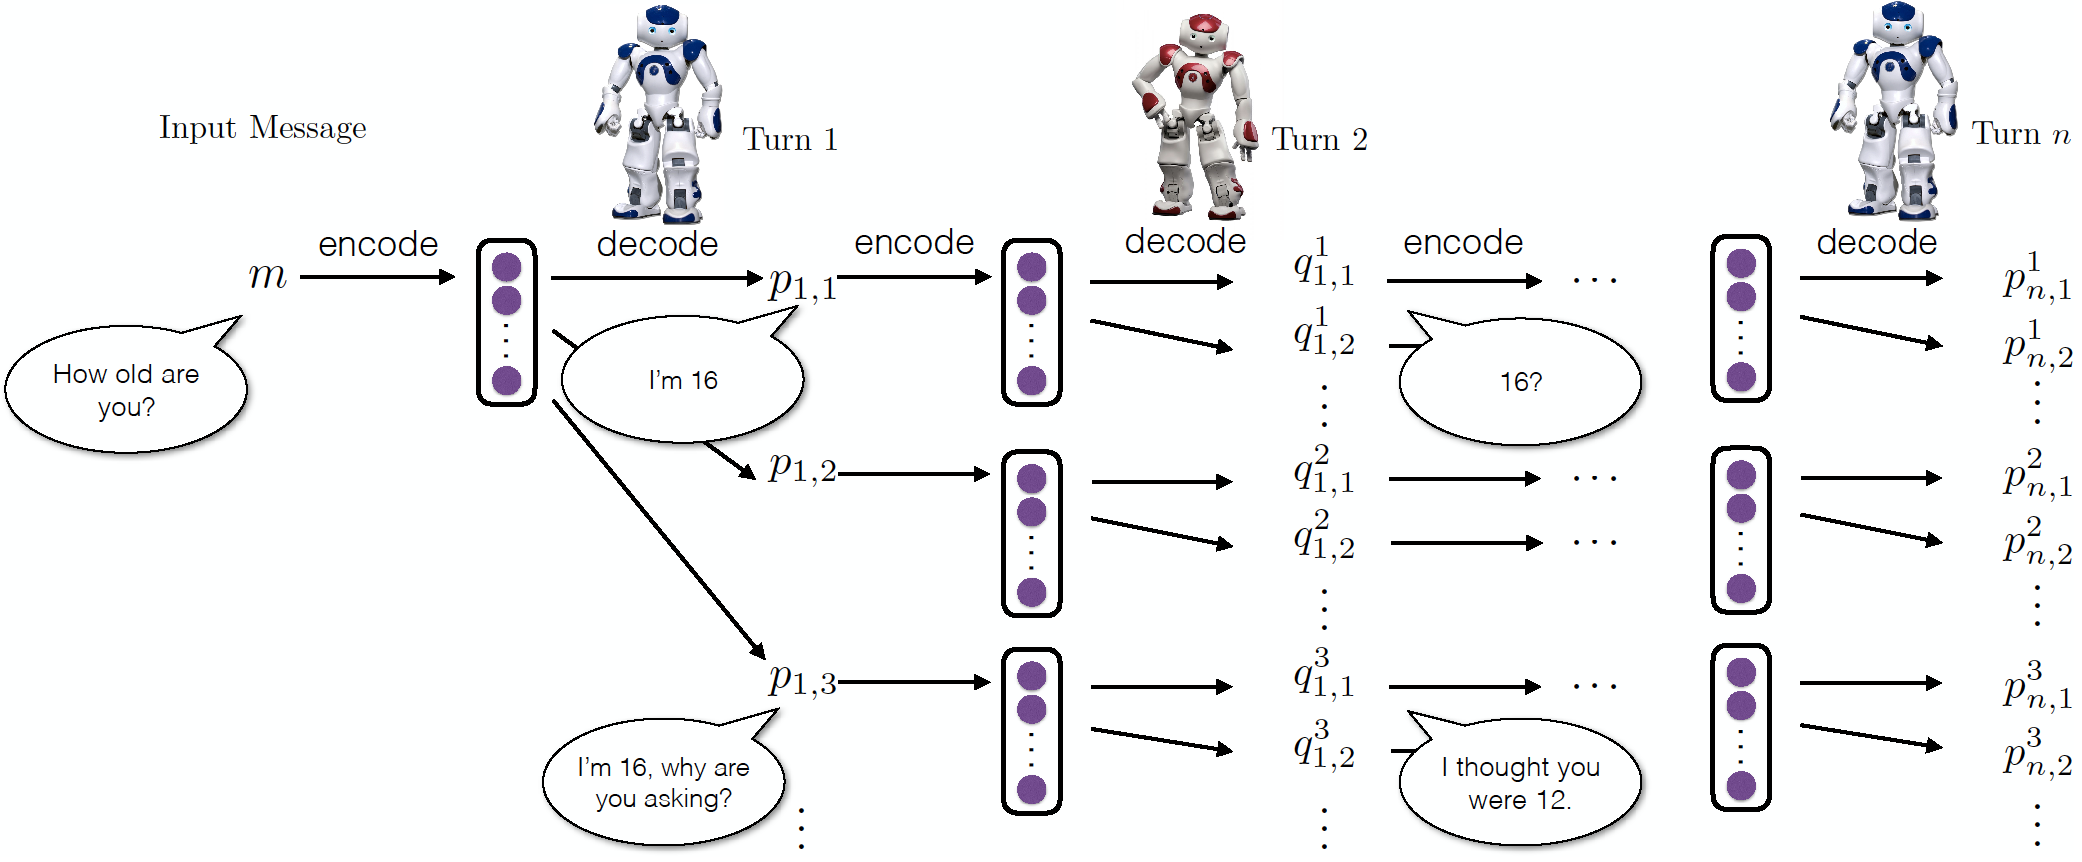
\includegraphics[width=1\textwidth]{thesis/chatbot/congtrinh/img/generation.png}
    \caption{Mô phỏng đối thoại giữa hai tác nhân}
    \label{fig:generation}
\end{figure}

Quá trình mô phỏng diễn ra như sau:

\begin{itemize}
    \item Ở bước đầu tiên, một thông báo từ tập huấn luyện được đưa
    đến tác nhân đầu tiên. Tác nhân mã hóa thông điệp đầu vào thành
    biểu diễn vec-tơ.
    \item Sau đó, bắt đầu giải mã để tạo ra đầu ra phản hồi.
    \item Kết hợp đầu ra ngay lập tức từ tác nhân đầu tiên với
    lịch sử đối thoại, tác nhân thứ hai cập nhật trạng thái
    bằng cách mã hóa lịch sử đối thoại thành một biểu diễn.
    \item Sau đó, sử dụng bộ giải mã RNN để tạo ra các phản hồi.
    \item Phản hồi được trả lại cho tác nhân đầu tiên và quá trình
    này được lặp đi lặp lại.
\end{itemize}

Kết quả thử nghiệm được lấy mẫu ở hình \ref{fig:generationdialog}
chứng minh rằng cách tiếp cận của họ thúc đẩy một cuộc đối thoại
bền vững hơn và quản lý để tạo ra nhiều phản hồi tương tác hơn
so với các mô hình SEQ2SEQ tiêu chuẩn được đào tạo bằng cách
sử dụng mục tiêu MLE.

\begin{figure}[ht]
    \centering
    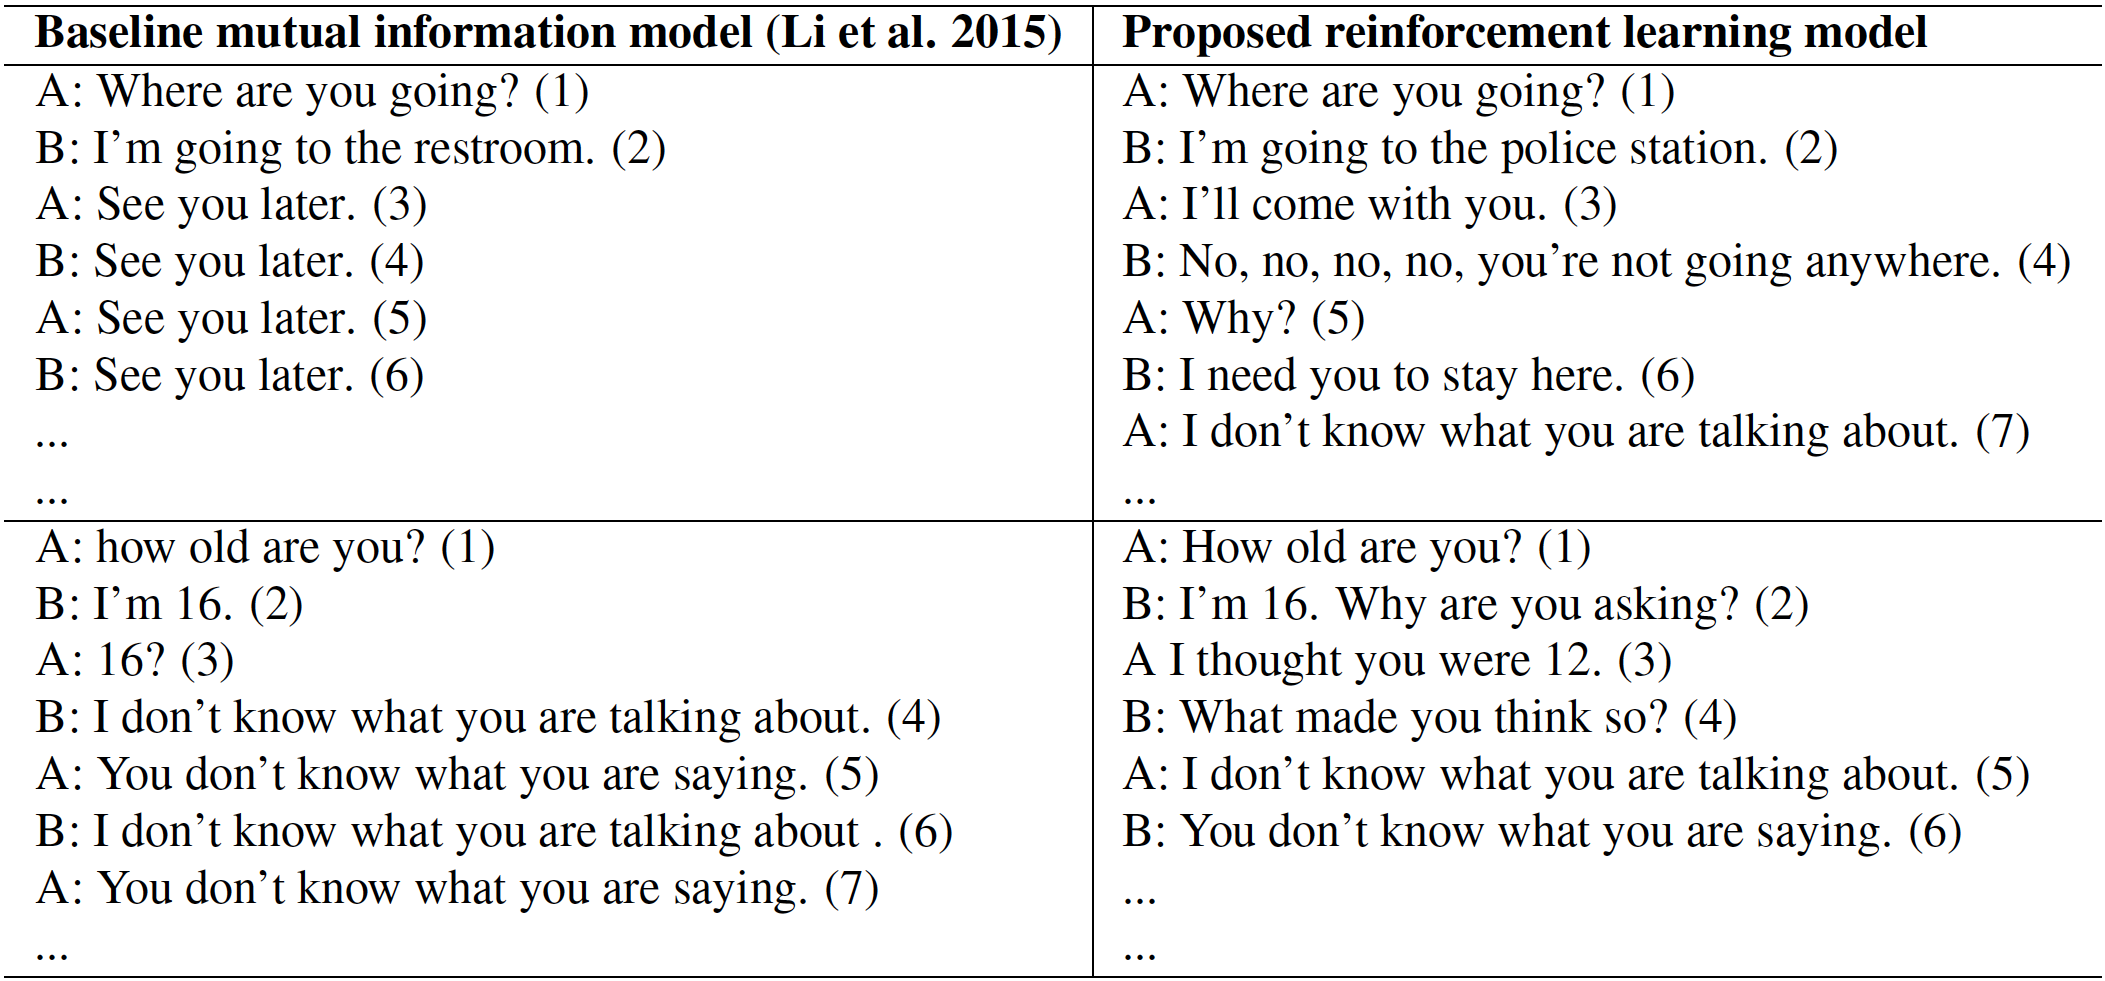
\includegraphics[width=1\textwidth]{thesis/chatbot/congtrinh/img/generationdialog.png}
    \caption{Kết quả thử nghiệm của hai mô hình}
    \label{fig:generationdialog}
\end{figure}

Cột bên trái: Mô phỏng đối thoại giữa hai tác nhân sử dụng bộ
mã hóa-giải mã LSTM 4 lớp được đào tạo trên tập dữ liệu
OpenSubtitles. Lượt đầu tiên (chỉ số 1) được nhập bởi các tác giả.
Sau đó, hai tác nhân thay phiên nhau trò chuyện, lấy đầu vào cho lượt
tạo trước của tác nhân kia. Cột Bên phải: Cuộc đối thoại được mô phỏng
bằng cách sử dụng mô hình học tập tăng cường được đề xuất. Mô hình mới
có nhiều cách nói hướng tới tương lai hơn (những câu hỏi như
\enquote{Why are you asking?} và những lời đề nghị như
\enquote{I'll come with you} giúp cuộc hội thoại diễn biến lâu hơn
trước khi rơi vào hố đen (black holes).

\subsection{Bài báo về Chatbot FAQ}
Đây là bài báo có tên \textit{Self-improving Chatbots based on
Reinforcement Learning} \cite{selfimproving}. Trong bài báo này,
họ giới thiệu mô hình học tăng cường (RL) cho các Chatbot tự
cải thiện, nhắm mục tiêu cụ thể đến các Chatbot dạng câu hỏi
thường gặp (FAQ).

Mô hình này không nhằm mục đích xây dựng hệ thống hội thoại từ đầu
mà nhằm tận dụng dữ liệu từ các cuộc trò chuyện của người dùng để
cải thiện hiệu suất Chatbot. Cốt lõi của phương pháp tiếp cận của họ
là mô hình điểm số, được đào tạo để tính điểm các câu trả lời của
Chatbot dựa trên phản hồi của người dùng. Điểm số được dự đoán bởi
mô hình này được sử dụng làm phần thưởng cho tác nhân. Việc học
chính sách diễn ra ngoại tuyến, nhờ vào trình mô phỏng người dùng
được cung cấp các câu thoại từ cơ sở dữ liệu FAQ. Học chính sách
được triển khai bằng cách sử dụng tác nhân Deep Q-Network (DQN) với
tính năng thăm dò tham lam (epsilon-greedy), được điều chỉnh để đưa
vào một cách hiệu quả các câu trả lời dự phòng cho các câu hỏi
ngoài phạm vi.

Kiến trúc mô hình được minh họa trong hình \ref{fig:selfimprovingarch}.

\begin{figure}[ht]
    \centering
    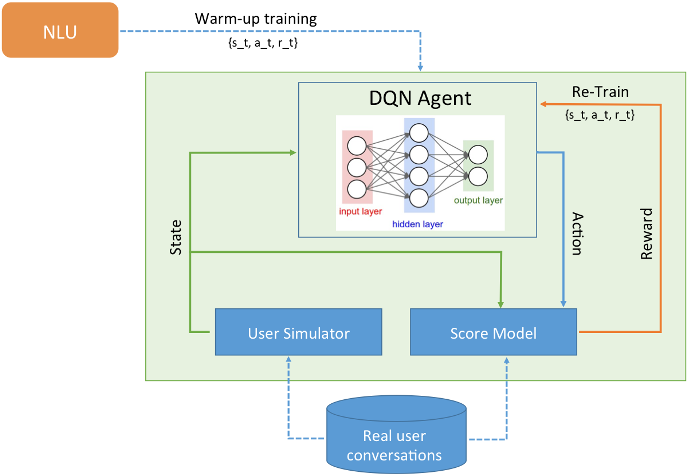
\includegraphics[width=1\textwidth]{thesis/chatbot/congtrinh/img/selfimproving_arch.png}
    \caption{Kiến trúc của mô hình Chatbot FAQ}
    \label{fig:selfimprovingarch}
\end{figure}

Các thành phần khác nhau của mô hình bao gồm:
\begin{itemize}
    \item Bộ hiểu ngôn ngữ tự nhiên (NLU), được sử dụng để huấn luyện
    tác nhân trong giai đoạn khởi động.
    \item Bộ mô phỏng người dùng (User Simulator), trích xuất
    ngẫu nhiên câu thoại của người dùng từ cơ sở dữ liệu về
    trải nghiệm người dùng.
    \item Mô hình điểm số (Score Model) được huấn luyện trên cuộc
    trò chuyện của người dùng với phản hồi và tác nhân dựa trên
    mạng Deep Q-Network (DQN).
\end{itemize}

Tác nhân DQN ban đầu được huấn luyện ngoại tuyến trong giai đoạn
khởi động với NLU. Mô hình điểm số cũng được huấn luyện ngoại tuyến
với dữ liệu từ các cuộc trò chuyện của người dùng thực. Trong
vòng lặp học tăng cường, trạng thái người dùng (lời phát biểu của
người dùng) được cung cấp bởi trình mô phỏng người dùng, hành động
(phản hồi chatbot) được cung cấp bởi tác nhân DQN và phần thưởng
được cung cấp bởi mô hình điểm. Mỗi tuple $(s_t, a_t, r_t)$ cung cấp
bộ đệm phát lại trải nghiệm (experience replay), được sử dụng để
huấn luyện lại DQN sau $n_{episodes}$ số lượt, là một tham số có thể
điều chỉnh được.

Tiềm năng của phương pháp tiếp cận của họ được thể hiện trên một
trường hợp nhỏ được trích xuất từ một Chatbot doanh nghiệp. Nó
cho thấy sự gia tăng hiệu suất từ tỷ lệ thành công 50\% ban đầu
lên 75\% trong 20-30 epoch huấn luyện.

\subsection{Chuỗi bài hướng dẫn huấn luyện Chatbot hướng mục tiêu
sử dụng học tăng cường}
\label{subsec:training}
Đây là chuỗi bài hướng dẫn \cite{traininggochatbot} được thực hiện
bởi một kênh nổi tiếng trên diễn đàn Medium - Towards Data Science.
Điểm nổi bật của chuỗi bài này là tác giả đã xây dựng được một
kiến trúc hệ thống học tăng cường (Reinforcement Learning) khá
hoàn thiện, áp dụng cho bài toán tư vấn có mục tiêu cụ thể. Đặc biệt,
có sử dụng hệ thống giả lập người dùng (User Simulator) với một số
luật đơn giản để giúp hệ thống học tăng cường có thể học được nhanh
hơn rất nhiều thay vì phải cần người thật tương tác. Những kiến thức
đó được tác giả vận dụng từ một bài báo \cite{endtoend} của nhóm
nghiên cứu đến từ phòng nghiên cứu của Microsoft, Hoa Kỳ. Cụ thể,
kiến trúc mà tác giả đề cập tới bao gồm bốn phần chính là
\textit{Agent} (tác nhân - đối tượng sẽ được huấn luyện để ra
quyết định), \textit{Dialog State Tracker} (đối tượng quản lý
trạng thái hội thoại), \textit{User Simulator} (đối tượng giả lập
người dùng - mục đích giúp quá trình huấn luyện nhanh chóng hơn) và
\textit{EMC - Error Model Controller} (mô phỏng lỗi - giúp tác nhân
học hiệu quả hơn).

Bài toán mà tác giả nêu ra trong bài viết của mình là tư vấn chọn vé
xem phim. Dữ liệu là các thông tin của xuất phim và được lưu dưới ở
dạng các cặp khóa - giá trị như biểu diễn ở ví dụ \ref{exam:dbmovie}.

\renewcommand{\textboxenvname}{Ví dụ}
\begin{textbox}[exam:dbmovie]{Dữ liệu thông tin của các xuất phim}
\begin{Verbatim}[breaklines=true, breakanywhere=true]
0L: {'city': 'hamilton', 'theater': 'manville 12 plex', 'zip': '08835', 'critic_rating': 'good', 'genre': 'comedy', 'state': 'nj', 'starttime': '10:30am', 'date': 'tomorrow', 'moviename': 'zootopia'}
897L: {'city': 'seattle', 'theater': 'pacific place 11', 'moviename': 'how to be single', 'zip': '98101', 'critic_rating': 'top', 'date': 'tonight', 'state': 'washington', 'other': 'date', 'starttime': '9', 'theater_chain': 'amc', 'genre': 'romance'}
\end{Verbatim}
\end{textbox}

Các khóa như \enquote{0L} hay \enquote{897L} là khóa định danh của
từng xuất phim có kiểu dữ liệu số nguyên và giá trị của nó cũng ở
dạng các cặp khóa - giá trị (một kiểu \textit{dictionary} trong
\textit{python}) có chứa các thông tin (city, theater, zip, v.v.).
Các xuất phim không có số lượng các thông tin giống nhau và các
giá trị của thông tin cũng khác nhau.

Ngoài ra, họ còn có một loại dữ liệu nữa là từ điển (database
dictionary) chứa tất cả các giá trị có thể có của từng thông tin với
mục đích là dùng cho bộ \textit{EMC} để tạo ra lỗi, cấu trúc được
biểu diễn như ở ví dụ \ref{exam:dictmovie}.

\renewcommand{\textboxenvname}{Ví dụ}
\begin{textbox}[exam:dictmovie]{Từ điển của các thông tin xuất phim}
\begin{Verbatim}[breaklines=true, breakanywhere=true]
'city': ['hamilton', 'manville', 'bridgewater', 'seattle', 'bellevue', 'birmingham', 'san francisco', 'portland', ...]
'theater': ['manville 12 plex', 'amc dine-in theatres bridgewater 7', 'bridgewater', 'every single theatre', ...]
\end{Verbatim}
\end{textbox}

Loại dữ liệu thứ ba được tác giả đề cập tới là danh sách mục tiêu
người dùng (user goal) chứa tất cả mục tiêu có thể có của người dùng
khi họ bắt đầu một cuộc hội thoại với Chatbot. Dữ liệu này sẽ được
\textit{User Simulator} sử dụng trong quá trình huấn luyện
\textit{agent}, cấu trúc bao gồm:

\begin{itemize}
    \item \textit{inform slots}: các thông tin người dùng sẽ cung cấp
    cho \textit{agent}.
    \item \textit{request slots}: các thông tin người dùng yêu cầu
    nhận được từ \textit{agent}.
\end{itemize}

\textit{Inform slots} và \textit{request slots} có thể có giá trị
hoặc rỗng. Cấu trúc được biểu diễn như ở ví dụ \ref{exam:goalmovie}.

\renewcommand{\textboxenvname}{Ví dụ}
\begin{textbox}[exam:goalmovie]{Mục tiêu người dùng của hệ thống tư vấn chọn vé xem phim}
\begin{Verbatim}[breaklines=true, breakanywhere=true]
{'request_slots': {'date': 'UNK', 'theater': 'UNK'}, 'inform_slots': {'numberofpeople': '4', 'moviename': 'zootopia', 'starttime': 'matinee'}}
{'request_slots': {'theater': 'UNK'}, 'inform_slots': {'city': 'la', 'numberofpeople': '2', 'distanceconstraints': 'downtown', 'video_format': '3d', 'starttime': '7pm', 'date': 'tomorrow', 'moviename': 'creed'}}
\end{Verbatim}
\end{textbox}

Một khái niệm được đề cập xuyên suốt gọi là \textit{action}.
\textit{Action} mô tả một hành động và dựa trên nó, ta có thể sinh ra
câu phản hồi. Hệ thống không làm việc trực tiếp với câu dưới dạng
ngôn ngữ tự nhiên mà thông qua \textit{action}. Một \textit{action}
sẽ có \textit{inform slots} và \textit{request slots} giống
\textit{user goal} như đã nêu ở trên đồng thời có thêm
\textit{intent} - ý định của người dùng hoặc của \textit{agent}
ứng với mỗi câu thoại diễn ra trong hội thoại. Với bài toán tư vấn
vé xem phim, tác giả đã định nghĩa các loại \textit{intent} như:

\begin{itemize}
    \item \textbf{Inform:} cung cấp những điều kiện ràng buộc,
    thông tin được trình bày trong \textit{inform slots}.
    \item \textbf{Request:} yêu cầu giá trị cho các thông tin được
    trình bày trong \textit{request slots}.
    \item \textbf{Thanks:} chỉ thực hiện bởi người dùng, thể hiện cho
    \textit{agent} biết rằng nó đã làm gì đó tốt hoặc người dùng đã
    sẵn sàng kết thúc cuộc hội thoại.
    \item \textbf{Match Found:} chỉ thực hiện bởi \textit{agent},
    thông báo cho người dùng biết rằng nó đã tìm được thông tin
    thỏa mãn các điều kiện ràng buộc của người dùng.
    \item \textbf{Reject:} chỉ thực hiện bởi người dùng, báo cho
    \textit{agent} biết rằng thông tin nó vừa thông báo không
    thỏa mãn yêu cầu ràng buộc của người dùng.
    \item \textbf{Done:} \textit{agent} sử dụng để báo rằng nó đã
    hoàn thành mục tiêu hội thoại. Người dùng sử dụng \textit{intent}
    này để kết thúc hội thoại.
\end{itemize}

Khái niệm đi kèm với \textit{action} là \textit{state} - trạng thái
của cuộc hội thoại. Nó đóng vai trò là đầu vào cho \textit{agent} để
chọn ra một \textit{action} phù hợp nhất. \textit{State} thực chất là
một ma trận mã hóa toàn bộ lịch sử hội thoại từ lúc bắt đầu cho tới
thời điểm hiện tại.

Hình \ref{fig:trainrefer} mô tả một vòng huấn luyện của hệ thống này
sẽ được diễn ra. Cụ thể:

\begin{figure}[ht]
    \centering
    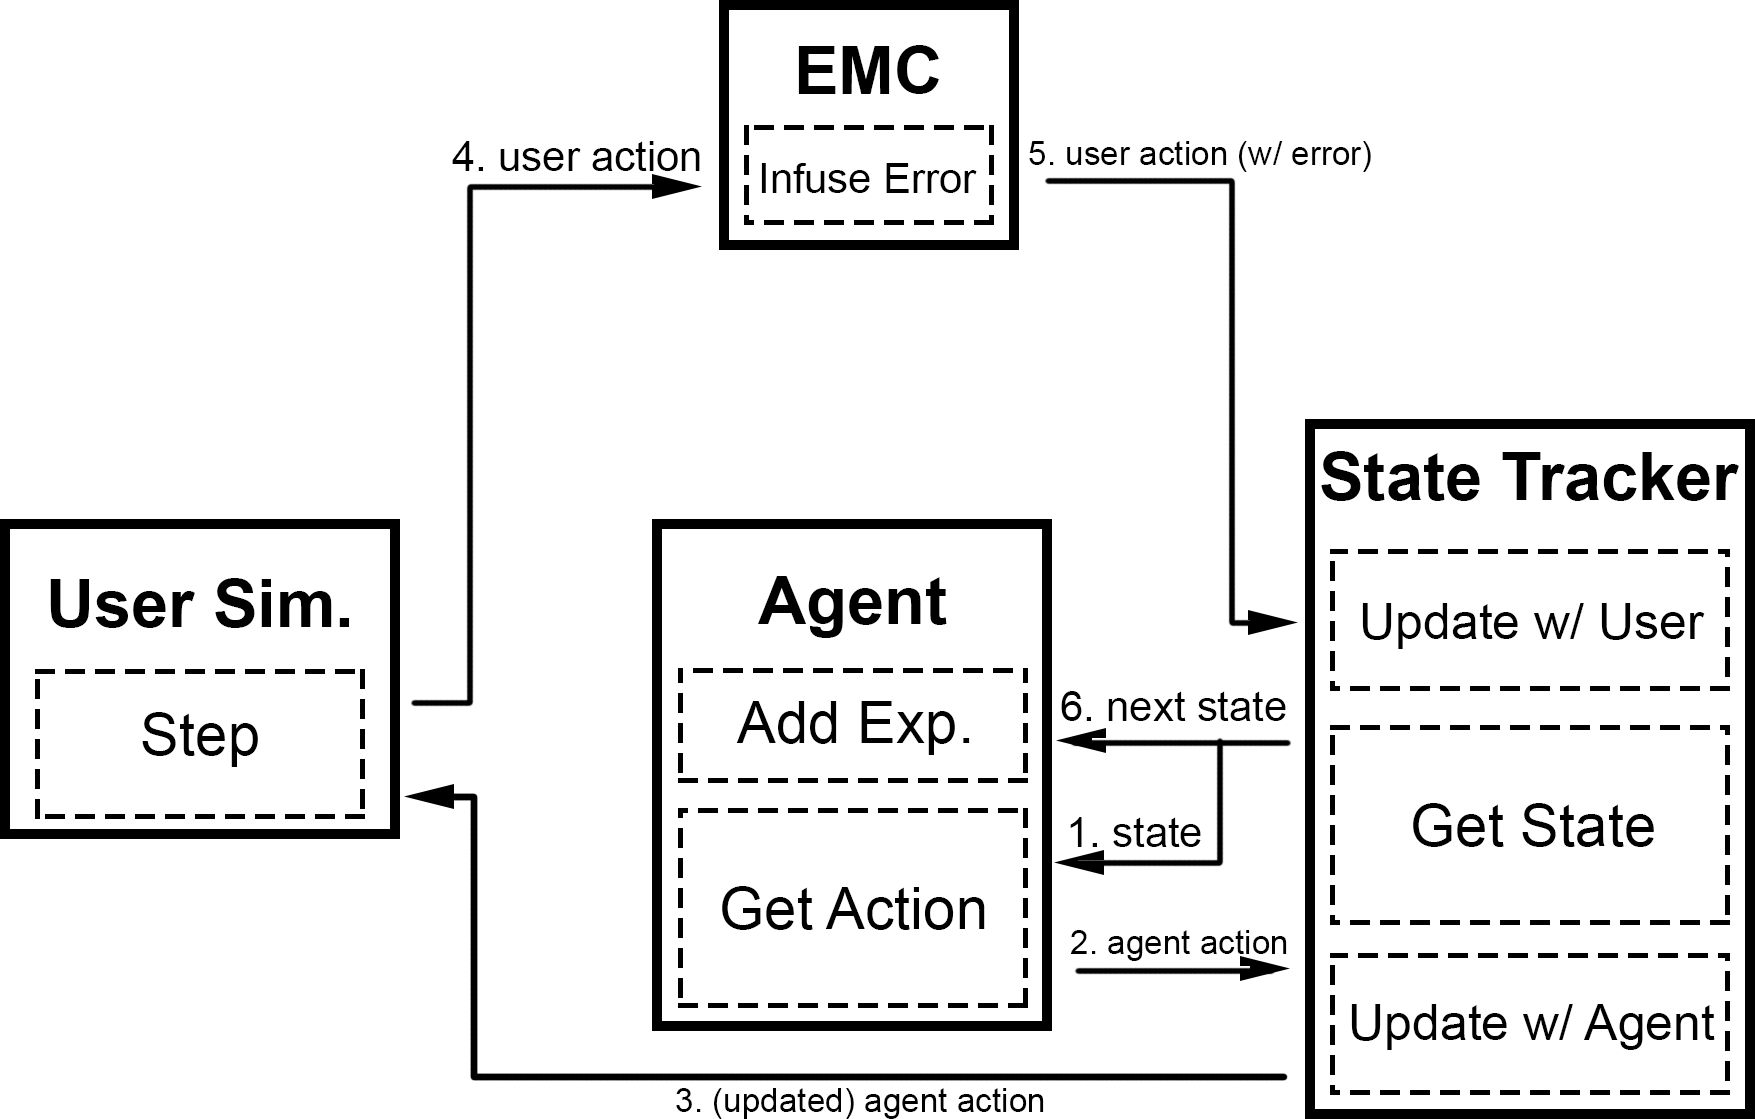
\includegraphics[width=1\textwidth]{thesis/chatbot/congtrinh/img/train_refer.png}
    \caption{Kiến trúc tổng quát của mô hình RL agent}
    \label{fig:trainrefer}
\end{figure}

\begin{itemize}
    \item \textbf{Bước 1:} Lấy ra \textit{state} - trạng thái hiện tại từ
    \textit{State Tracker}, \textit{state} này có thể là \textit{state}
    khởi tạo nếu như vừa bắt đầu hội thoại hoặc là \textit{state} của
    toàn bộ cuộc hội thoại giữa người dùng và Chatbot. \textit{State}
    sau khi được lấy ra sẽ làm đầu vào (input) cho \textit{agent} ở
    bước tiếp theo.
    \item \textbf{Bước 2:} \textit{Agent} sau khi nhận được input từ
    bước trước sẽ sinh ra \textit{action} và gửi ngược về lại
    \textit{State Tracker}. \textit{Action} lúc này ở dạng thô, chưa
    kèm thông tin cụ thể. Nó sẽ được \textit{State Tracker} cập nhật
    thông tin sau khi thực hiện truy vấn lên cơ sở dữ liệu. Đồng thời
    \textit{State Tracker} cũng sẽ cập nhật lại trạng thái của hội thoại.
    \item \textbf{Bước 3:} \textit{Action} sau khi được cập nhật
    đầy đủ thông tin sẽ được gửi cho \textit{User Simulator}.
    \textit{User Simulator} sẽ dựa vào các luật đã được quy định trước
    để sinh ra \textit{action} (có cấu trúc tương tự \textit{action}
    của \textit{agent} ở bước trước), kèm theo \textit{reward}
    (điểm thưởng) và tín hiệu success (thành công) để giúp
    \textit{agent} có thể tự điều chỉnh hành vi để học.
    \item \textbf{Bước 4:} \textit{Action} của người dùng ở bước
    trước đó sẽ được đưa qua \textit{EMC}, mục đích là tạo ra các lỗi
    mà người dùng thật hay mắc phải, giúp \textit{agent} có hành vi
    chính xác và tự nhiên hơn khi chạy ở thực tế.
    \item \textbf{Bước 5:} \textit{Action} ở bước trước sẽ tiếp tục
    được gửi đi đến \textit{State Tracker} và được cập nhật thông tin
    cụ thể tương tự ở bước 2. Đồng thời \textit{State Tracker} cũng
    cập nhật trạng thái của nó.
    \item \textbf{Bước 6:} Trạng thái tiếp theo được lấy từ
    \textit{State Tracker} và quay lại giống bước 1.
\end{itemize}

\section{Kết luận}
Hiện nay, có rất nhiều nghiên cứu, công trình liên quan đến xây dựng
một Chatbot tư vấn khách hàng trong nhiều lĩnh vực cũng như các
nghiên cứu cụ thể liên quan đến mô hình sử dụng học tăng cường như
đã trình bày ở một số công trình ở trên.

Trong đó, các công trình xây dựng Chatbot cho các dịch vụ tư vấn
sử dụng các phương pháp đa dạng, từ đơn giản như sử dụng cấu trúc
ngôn ngữ và so trùng cho đến áp dụng các bộ xử lý ngôn ngữ tự nhiên,
huấn luyện mô hình hay để tiết kiệm nguồn lực và chi phí sử dụng
các nền tảng sẵn có. Việc này cũng tùy thuộc vào lĩnh vực của
Chatbot hoạt động.

Các hướng tiếp cận sử dụng mô hình học tăng cường cũng được áp dụng
trên nhiều lĩnh vực khác nhau. Kết quả của những nghiên cứu trên
cũng thể hiện được điểm mạnh của mô hình này. Các tác nhân có các
phản hồi linh hoạt hơn, với cơ chế tự học cũng giúp nó không
giới hạn khả năng. Lý giải tại sao giải thuật học tăng cường được
áp dụng mạnh mẽ trong các hệ thống Chatbot. Vì vậy trong luận văn
này cũng đã áp dụng phương pháp này. Cụ thể, đề tài tham khảo một
kiến trúc huấn luyện mô hình học tăng cường hướng mục tiêu được
trình bày ở mục \ref{subsec:training}.

\chapter{Kiến thức nền tảng}

\section{Học tăng cường (Reinforcement Learning)}

\subsection{Giới thiệu}
Học tăng cường (Reinforcement Learning)
\cite{reinforcementlearninganintroduction} là học cách ánh xạ các
tình huống thành hành động để cực đại phần thưởng. Người học
không được cho biết hành động nào cần thực hiện, nhưng thay vào đó
phải khám phá ra hành động nào mang lại nhiều phần thưởng nhất
bằng cách thử chúng. Trong những trường hợp thú vị và khó khăn nhất,
các hành động có thể không chỉ ảnh hưởng đến phần thưởng mà còn
ảnh hưởng đến tình huống tiếp theo và thông qua đó, cũng ảnh hưởng
đến tất cả các phần thưởng tiếp theo. Hai đặc điểm này —
tìm kiếm thử-và-sửa sai (trial-and-error) và trì hoãn phần thưởng —
là hai đặc điểm phân biệt quan trọng nhất của học tăng cường.

\subsection{Các thành phần của học tăng cường}
Ngoài \textit{agent} (tác nhân) và \textit{environment} (môi trường),
người ta có thể xác định bốn thành phần chính của hệ thống
học tăng cường: \textit{policy} (chính sách), \textit{reward signal}
(tín hiệu phần thưởng), \textit{value function} (hàm giá trị),
và có thể có thêm \textit{model} (mô hình) của môi trường.

\begin{itemize}
    \item \textbf{Policy:} xác định cách hoạt động của tác nhân tại
    một thời điểm nhất định. Nói một cách đại khái, một
    \textit{policy} là một ánh xạ từ các trạng thái nhận thức của
    môi trường đến các hành động sẽ được thực hiện khi ở trong các
    trạng thái đó. Nó tương ứng với những gì trong tâm lý học sẽ được
    gọi là một tập hợp các quy tắc hoặc liên kết kích thích-phản ứng.
    Trong một số trường hợp, \textit{policy} có thể là một hàm hoặc
    bảng tra cứu đơn giản, trong khi trong những trường hợp khác,
    \textit{policy} có thể liên quan đến tính toán mở rộng chẳng hạn
    như quá trình tìm kiếm. \textit{Policy} là cốt lõi của một
    tác nhân học tăng cường theo nghĩa là chỉ nó là đủ để xác định
    hành vi. Nói chung, các \textit{policy} có thể ngẫu nhiên,
    chỉ rõ xác suất cho mỗi hành động.
    \item \textbf{Reward signal:} xác định mục tiêu trong vấn đề
    học tăng cường. Trên mỗi bước thời gian, môi trường gửi cho
    tác nhân một số duy nhất được gọi là phần thưởng. Mục tiêu
    duy nhất của tác nhân là tối đa hóa tổng phần thưởng mà tác nhân
    nhận được trong thời gian dài. Do đó, \textit{reward signal}
    xác định đâu là những sự kiện tốt và xấu đối với tác nhân.
    Trong một hệ thống sinh học, chúng ta có thể nghĩ về phần thưởng
    tương tự như trải nghiệm của niềm vui hoặc nỗi đau. Chúng là các
    đặc điểm tức thời và xác định vấn đề mà tác nhân phải đối mặt.
    \textit{Reward signal} là cơ sở chính để thay đổi \textit{policy};
    nếu một hành động được \textit{policy} chọn theo sau là
    \textit{reward} thấp, thì \textit{policy} có thể được thay đổi
    để chọn một số hành động khác trong tình huống đó trong tương lai.
    Nói chung, các \textit{reward signal} có thể là các hàm ngẫu nhiên
    của trạng thái môi trường và các hành động được thực hiện.
    \item \textbf{Value function:} Trong khi \textit{reward signal}
    cho biết điều gì tốt theo nghĩa tức thời, thì một
    \textit{value function} chỉ định điều gì tốt về lâu dài.
    Nói một cách đại khái, \textit{value} của một trạng thái là tổng
    số phần thưởng mà một tác nhân có thể mong đợi tích lũy trong
    tương lai, bắt đầu từ trạng thái đó. Trong khi \textit{reward}
    xác định mong muốn ngay lập tức, nội tại của các trạng thái
    môi trường, thì các \textit{value} cho thấy mong muốn lâu dài
    của các trạng thái sau khi tính đến các trạng thái có khả năng
    tuân theo và \textit{reward} có sẵn trong các trạng thái đó.
    Ví dụ: một trạng thái có thể luôn mang lại \textit{reward} tức thì
    thấp nhưng vẫn có \textit{value} cao vì nó thường xuyên được
    theo sau bởi các trạng thái khác mang lại \textit{reward} cao.
    Hoặc điều ngược lại có thể đúng. Để so sánh giữa con người với
    con người, \textit{reward} có phần giống như niềm vui (nếu cao)
    và nỗi đau (nếu thấp), trong khi \textit{value} tương ứng với sự
    đánh giá tinh tế hơn và có tầm nhìn xa hơn về mức độ hài lòng
    hoặc không hài lòng của chúng ta khi môi trường của chúng ta
    đang ở trong một trạng thái cụ thể.
    \item \textbf{Model environment:} Đây là thứ bắt chước hành vi
    của môi trường, hay nói chung hơn, cho phép đưa ra các suy luận
    về cách môi trường sẽ hoạt động. Ví dụ: với một trạng thái và
    hành động, mô hình có thể dự đoán trạng thái kết quả tiếp theo
    và phần thưởng tiếp theo. Mô hình được sử dụng để lập kế hoạch,
    theo đó chúng ta có thể quyết định một quá trình hành động
    bằng cách xem xét các tình huống có thể xảy ra trong tương lai
    trước khi chúng thực sự trải qua.
\end{itemize}

\subsection{Ứng dụng của học tăng cường}
Do tính chất của việc học tăng cường là luôn tối ưu việc đạt được
phần thưởng cuối cùng dựa vào trạng thái, và phần thưởng hiện tại,
cùng với sự tác động của môi trường nên việc học tăng cường được
áp dụng nhiều trong các lĩnh vực mang đậm tính tương tác lâu dài
giữa tác nhân và môi trường, có thể kể đến:

\begin{itemize}
    \item Điều khiển xe tự hành, robot, v.v.
    \item Các hệ thống gợi ý (Recommendation System), hỏi đáp
    (Chatbot), v.v.
    \item Ngành công nghiệp trò chơi (game) như là cờ vây
    (nổi tiếng với AlphaGo), v.v.
\end{itemize}

Cụ thể, trong luận án này sẽ sử dụng phương pháp học tăng cường
cho việc huấn luyện mô hình tư vấn khách hàng.

\section{Hệ thống Chatbot hướng mục tiêu (Goal Oriented)}

\subsection{Chatbot hướng mục tiêu}
\label{subsec:chatbotgo}
Yêu cầu của một hệ thống tư vấn khách hàng là ta phải đặt cho nó
một ngữ cảnh (tư vấn cái gì) và mục tiêu cuối cùng cần hoàn thành
khi tư vấn. Vì vậy, đây là một bài toán hướng mục tiêu.

Một Chatbot hướng mục tiêu (GO) cố gắng giải quyết một vấn đề
cụ thể cho người dùng. Các Chatbot này có thể giúp mọi người đặt vé,
tìm đặt chỗ, v.v. Có hai cách chính để huấn luyện một Chatbot GO:
Học có giám sát (supervised learning) với bộ mã hóa-giải mã
(encoder-decoder), ánh xạ trực tiếp cuộc đối thoại của người dùng
tới phản hồi và học tăng cường giúp huấn luyện một Chatbot
thông qua các cuộc hội thoại thử-và-sửa sai (trial-and-error) với
người dùng thực hoặc trình mô phỏng người dùng có quy tắc.

Như đã nói từ phần trước, luận án này sử dụng mô hình học tăng cường
vì các tối đa lợi thế của nó.

\subsection{Kiến trúc tổng quát của hệ thống Chatbot GO}
Hệ thống đối thoại cho một Chatbot GO sử dụng phương pháp
học tăng cường được chia thành 3 phần chính, được mô tả như hình
\ref{fig:chatbot}: Phần Quản lý hội thoại (Dialogue Manager), phần
Hiểu ngôn ngữ tự nhiên (Natural Language Understanding) và phần
Trình tạo ngôn ngữ tự nhiên (Natural Language Generator). Phần
Quản lý hội thoại được chia thành Bộ theo dõi trạng thái hội thoại
(Dialogue State Tracker) và \textit{policy} cho chính tác nhân, được
đại diện bởi mạng nơ-ron (neural network) trong nhiều trường hợp.
Ngoài ra, vòng lặp hệ thống chứa một người dùng với các mục tiêu.
Mục tiêu người dùng thể hiện những gì người dùng muốn để thoát khỏi
cuộc trò chuyện.

\begin{figure}[ht]
    \centering
    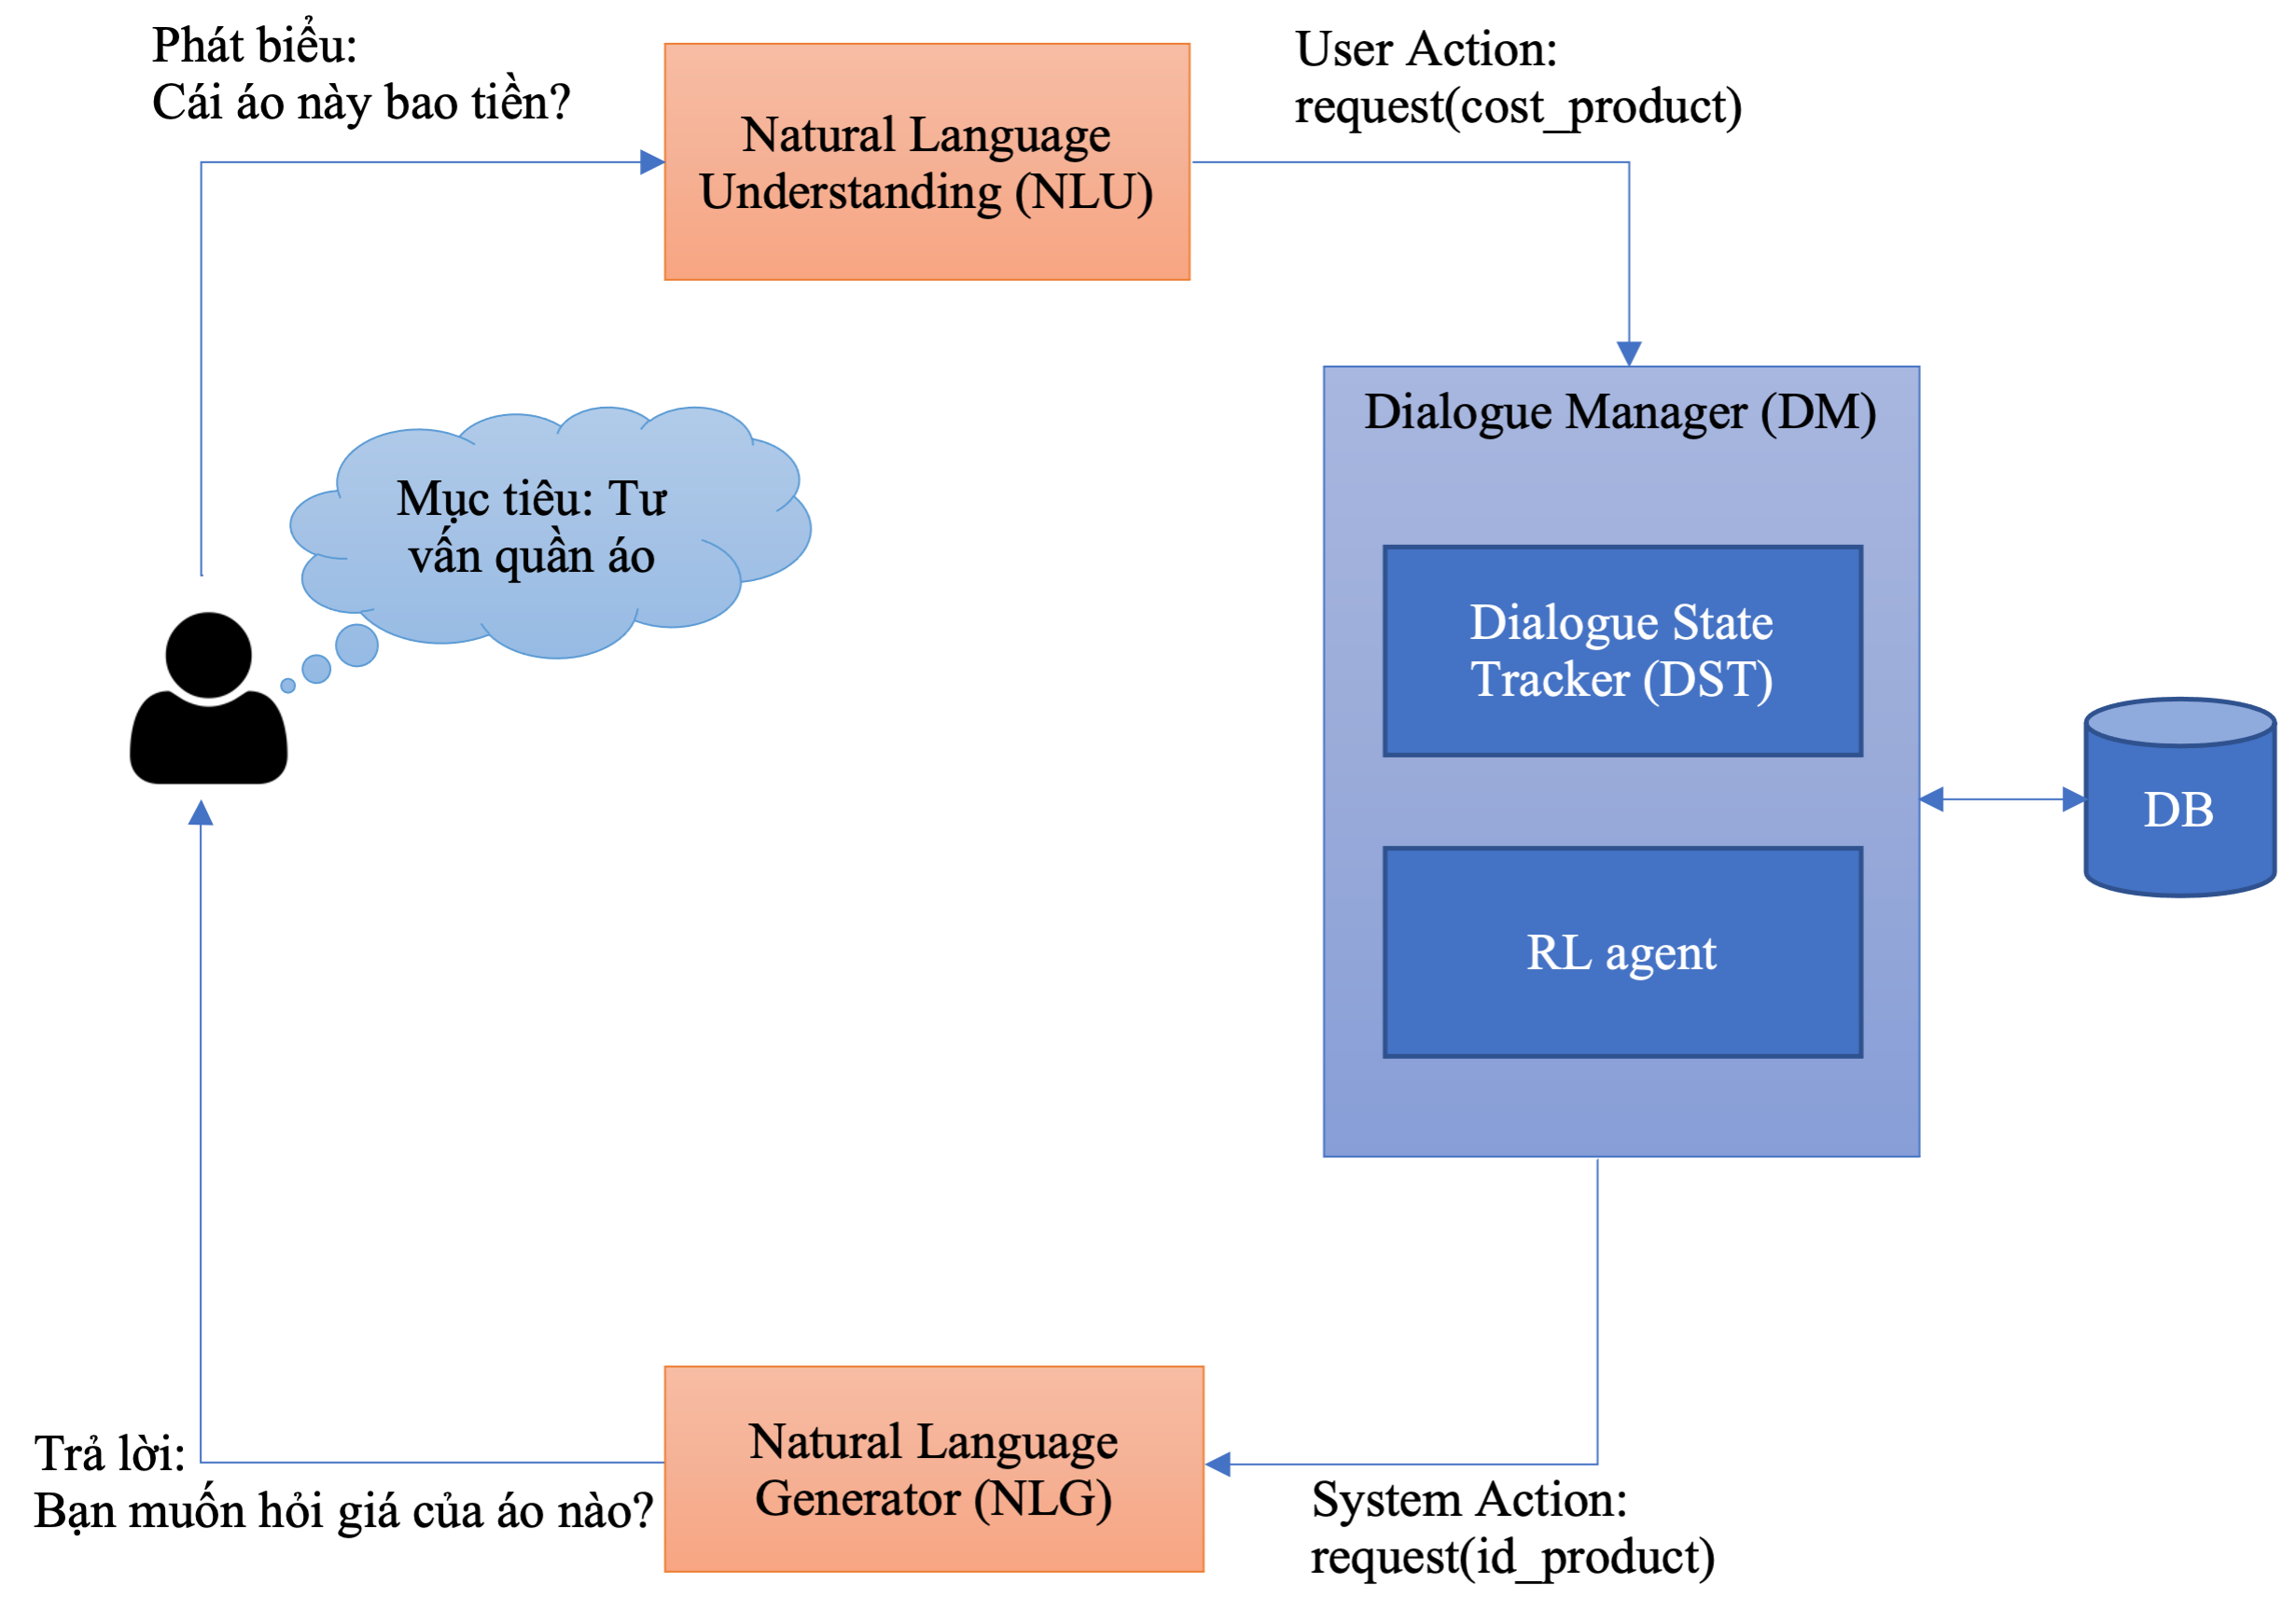
\includegraphics[scale=0.8]{thesis/chatbot/kienthuc/img/overviewchatbot.png}
    \caption{Kiến trúc tổng quát của mô hình Chatbot GO sử dụng
    phương pháp học tăng cường}
    \label{fig:chatbot}
\end{figure}

Khi người dùng gửi đi một thông điệp (Cái áo này bao tiền?), sẽ được
xử lý bởi thành phần Hiểu ngôn ngữ tự nhiên (NLU), chuyển ngôn ngữ
tự nhiên thành một dạng mà tác nhân có thể xử lý, đầu ra (output) là
ở dạng khung ngữ nghĩa (semantic frame) (request(cost\_product)).

Sau đó, Bộ theo dõi trạng thái đối thoại (DST) từ hành động của
người dùng (đã được chuyển thành khung ngữ nghĩa) và lịch sử của
cuộc trò chuyện hiện tại sẽ xử lý và chuyển thành một biểu diễn
trạng thái mà có thể xử lý được bởi \textit{policy} của tác nhân.
Trạng thái này là đầu vào của \textit{policy} hoặc mạng nơ ron của
tác nhân, đầu ra là hành động của tác nhân dưới dạng khung ngữ nghĩa
(request(id\_product)).

Cơ sở dữ liệu được truy vấn để thêm thông tin vào cho tác nhân như
thông tin các kích thước, màu sắc v.v.

Hành động của tác nhân sau đó được xử lý bởi phần Trình tạo ngôn ngữ
tự nhiên (NLG), chuyển nó sang ngôn ngữ tự nhiên để người dùng có thể
dễ dàng đọc hiểu (Bạn muốn hỏi giá của áo nào?).

\section{Mô hình học tăng cường cho Chatbot GO}
\label{sec:model}
Như đã đề cập ở mục giới hạn của đề tài \ref{sec:scope}, chúng ta sẽ
quan tâm sử dụng mô hình học tăng cường như thế nào để áp dụng vào
bài toán hướng mục tiêu tư vấn khách hàng. Trình bày ở mục
\ref{subsec:chatbotgo}, một tác nhân Chatbot hướng mục tiêu (GO) sẽ
được huấn luyện để trò chuyện thành thạo với người dùng thực nhằm
hoàn thành mục tiêu, phù hợp với các ràng buộc của người dùng.
Quá trình tác nhân học tập theo phương pháp học tăng cường được mô tả
rõ hơn ở hình \ref{fig:learningflow}.

\begin{figure}[ht]
    \centering
    
\includegraphics[scale=1]{thesis/chatbot/kienthuc/img/learningflow.png}
    \caption{Quá trình huấn luyện theo phương pháp học tăng cường}
    \label{fig:learningflow}
\end{figure}

Bản chất của học tăng cường là thử và sửa sai, nó sẽ thử đi thử lại
các hành động và rút ra kinh nghiệm sau mỗi lần thử. Trong bài toán
tư vấn khách hàng, việc thử này sẽ được thực hiện như sau:

\begin{itemize}
    \item Tại trạng thái hiện tại là $S_t$, tác nhân ngẫu nhiên hoặc
    theo một luật (policy) nào đó có sẵn chọn ra một hành động $A_t$.
    \item Hành động này sẽ tác động vào môi trường là diễn biến của
    hội thoại hiện tại cho ra trạng thái mới là $S_{t+1}$ và nhận
    giá trị là phần thường $R_t$ cho hành động đó.
    \item Phần thưởng này sẽ đánh giá được việc chọn hành động đó có
    tốt hay không. Từ đó tác nhân cập nhật lại cách chọn hành động.
\end{itemize}

Với mô hình này, ta dễ thấy tác nhân sẽ chỉ nhận đầu vào là
trạng thái hội thoại hiện tại để ra quyết định hành động.
Vì vậy, ta cần xem xét đến các thông tin cần có trong trạng thái
như thế nào để tác nhân có đủ thông tin để ra quyết định.
Việc này được trình bày rõ hơn trong mục \ref{subsec:state}.

Trong thời gian đầu, tác nhân có thể ngẫu nhiên chọn các hành động
hoặc theo một luật định sẵn đơn giản. Sau đó, nó cần được chỉ ra
hành động nào là không tốt, để cập nhập cách chọn hành động (policy),
cách thức thực hiện là thông qua điểm thưởng. Các điểm thưởng sẽ được
định nghĩa sao cho giống với các yêu cầu của người dùng thật để
quá trình tự học của tác nhân là hiệu quả và thỏa mãn với nhu cầu
người dùng. Cụ thể được mô tả trong mục \ref{subsec:reward}.

\subsection{Trạng thái hội thoại}
\label{subsec:state}
Trạng thái hội thoại chứa những thông tin hữu ích từ lịch sử
hội thoại cho tới thời điểm hiện tại. Các thông tin này có thể
khác nhau tùy vào mục đích sử dụng tác nhân. Tuy nhiên, nó nên chứa
các thông tin biểu thị tình trạng, những diễn biến đã, đang diễn ra
trong hội thoại. Dưới đây diễn giải một số thông tin trong trạng thái
hội thoại cho tác nhân trợ lý mua sắm.

Giả sử, ta có một cuộc hội thoại giữa người dùng và cửa hàng
diễn ra như sau:

\renewcommand{\textboxenvname}{Ví dụ}
\begin{textbox}[exam:dialog1]{Một mẫu đoạn hội thoại}
\begin{Verbatim}[breaklines=true, breakanywhere=true]
User: Hi shop
Admin: Chào bạn, bạn cần shop tư vấn sản phẩm nào ạ?
User: Chân váy hoa có size gì vậy bạn
Admin: Dạ chân váy hoa bên em có size M, và L ạ
User: Còn màu hồng ko?
Admin: Dạ sản phẩm còn 2 cái ạ
User: OK shop. Mình lấy cái này nha.
Admin: Bạn mặc size gì ạ?
\end{Verbatim}
\end{textbox}

Tại dòng 3, người dùng hỏi kích thước của sản phẩm. Để tác nhân
có thể thực hiện được hành vi đúng là cung cấp thông tin thì nó
cần biết rằng yêu cầu hiện tại của người dùng là gì (yêu cầu
thông tin kích thước) và thông tin người dùng cung cấp (tên
sản phẩm). Vì vậy, trạng thái hội thoại cần chứa hành động
hiện tại của người dùng.

Tại dòng 5, người dùng yêu cầu thông tin số lượng và cung cấp
thông tin màu sắc. Tuy nhiên, ta biết rằng để tìm kiếm đúng sản phẩm
phù hợp, cần biết tên của sản phẩm. Mà tên sản phẩm đã được
người dùng cung cấp tại dòng 3. Vì vậy, ngoài hành động hiện tại,
trạng thái hội thoại còn chứa tất cả các thông tin mà người dùng đã
thông báo trước đó.

Tại dòng 7, người dùng muốn đặt đơn hàng. Để chốt được đơn hàng,
cửa hàng cần biết đầy đủ thông tin cần thiết của sản phẩm để tìm thấy
một mẫu sản phẩm duy nhất. Như ví dụ trên, chân váy hoa có 2 loại
kích cỡ khác nhau. Tác nhân cần yêu cầu người dùng cung cấp thêm
thông tin này. Vì vậy trong trạng thái hội thoại cần có kết quả
sau khi truy vấn cơ sở dữ liệu của từng thông tin.

Ngoài ra, ta cần có thêm hành động gần nhất của tác nhân để tránh
việc lặp lại hành động từ tác nhân. Trong nhu cầu thực tế, việc
tư vấn và giúp người dùng đạt mục tiêu cuối cùng nên diễn ra
nhanh nhất có thể. Vì vậy, số lượt hội thoại đã diễn ra
cũng được thêm vào.

\subsection{Phần thưởng và ảnh hưởng của nó đến quyết định hành động}
\label{subsec:reward}
Ta cần định nghĩa phần thưởng phù hợp cho hành động của tác nhân
trong mỗi trạng thái hội thoại khác nhau. Xét ví dụ
\ref{exam:dialog1}, ta có thể định nghĩa một số điểm thưởng
dựa trên phản hồi của người dùng như sau:

\begin{itemize}
    \item Tại dòng 2, hành động của tác nhân đơn giản là chào hỏi lại
    người dùng. Hành động này thông thường và phản hồi của người dùng
    là tiếp nối cuộc trò chuyện. Vì vậy, hành động này có thể xem là
    hành động qua lượt, không mang giá trị điểm thưởng.
    \item Tại dòng 4, tác nhân cung cấp thông tin mà người dùng
    yêu cầu từ câu trước, hành động này không bị từ chối bởi
    người dùng ở câu sau. Vì vậy, hành động này xem là cung cấp
    giá trị có ích cho người dùng và được 1 điểm thưởng.
\end{itemize}

Sau khi có điểm thưởng cho từng hành động, việc tác nhân cập nhật
cách chọn hành động và đưa ra hành động mới như thế nào, ta xét
ví dụ sau như hình \ref{fig:dialog2}.

\begin{figure}[!ht]
    \centering
    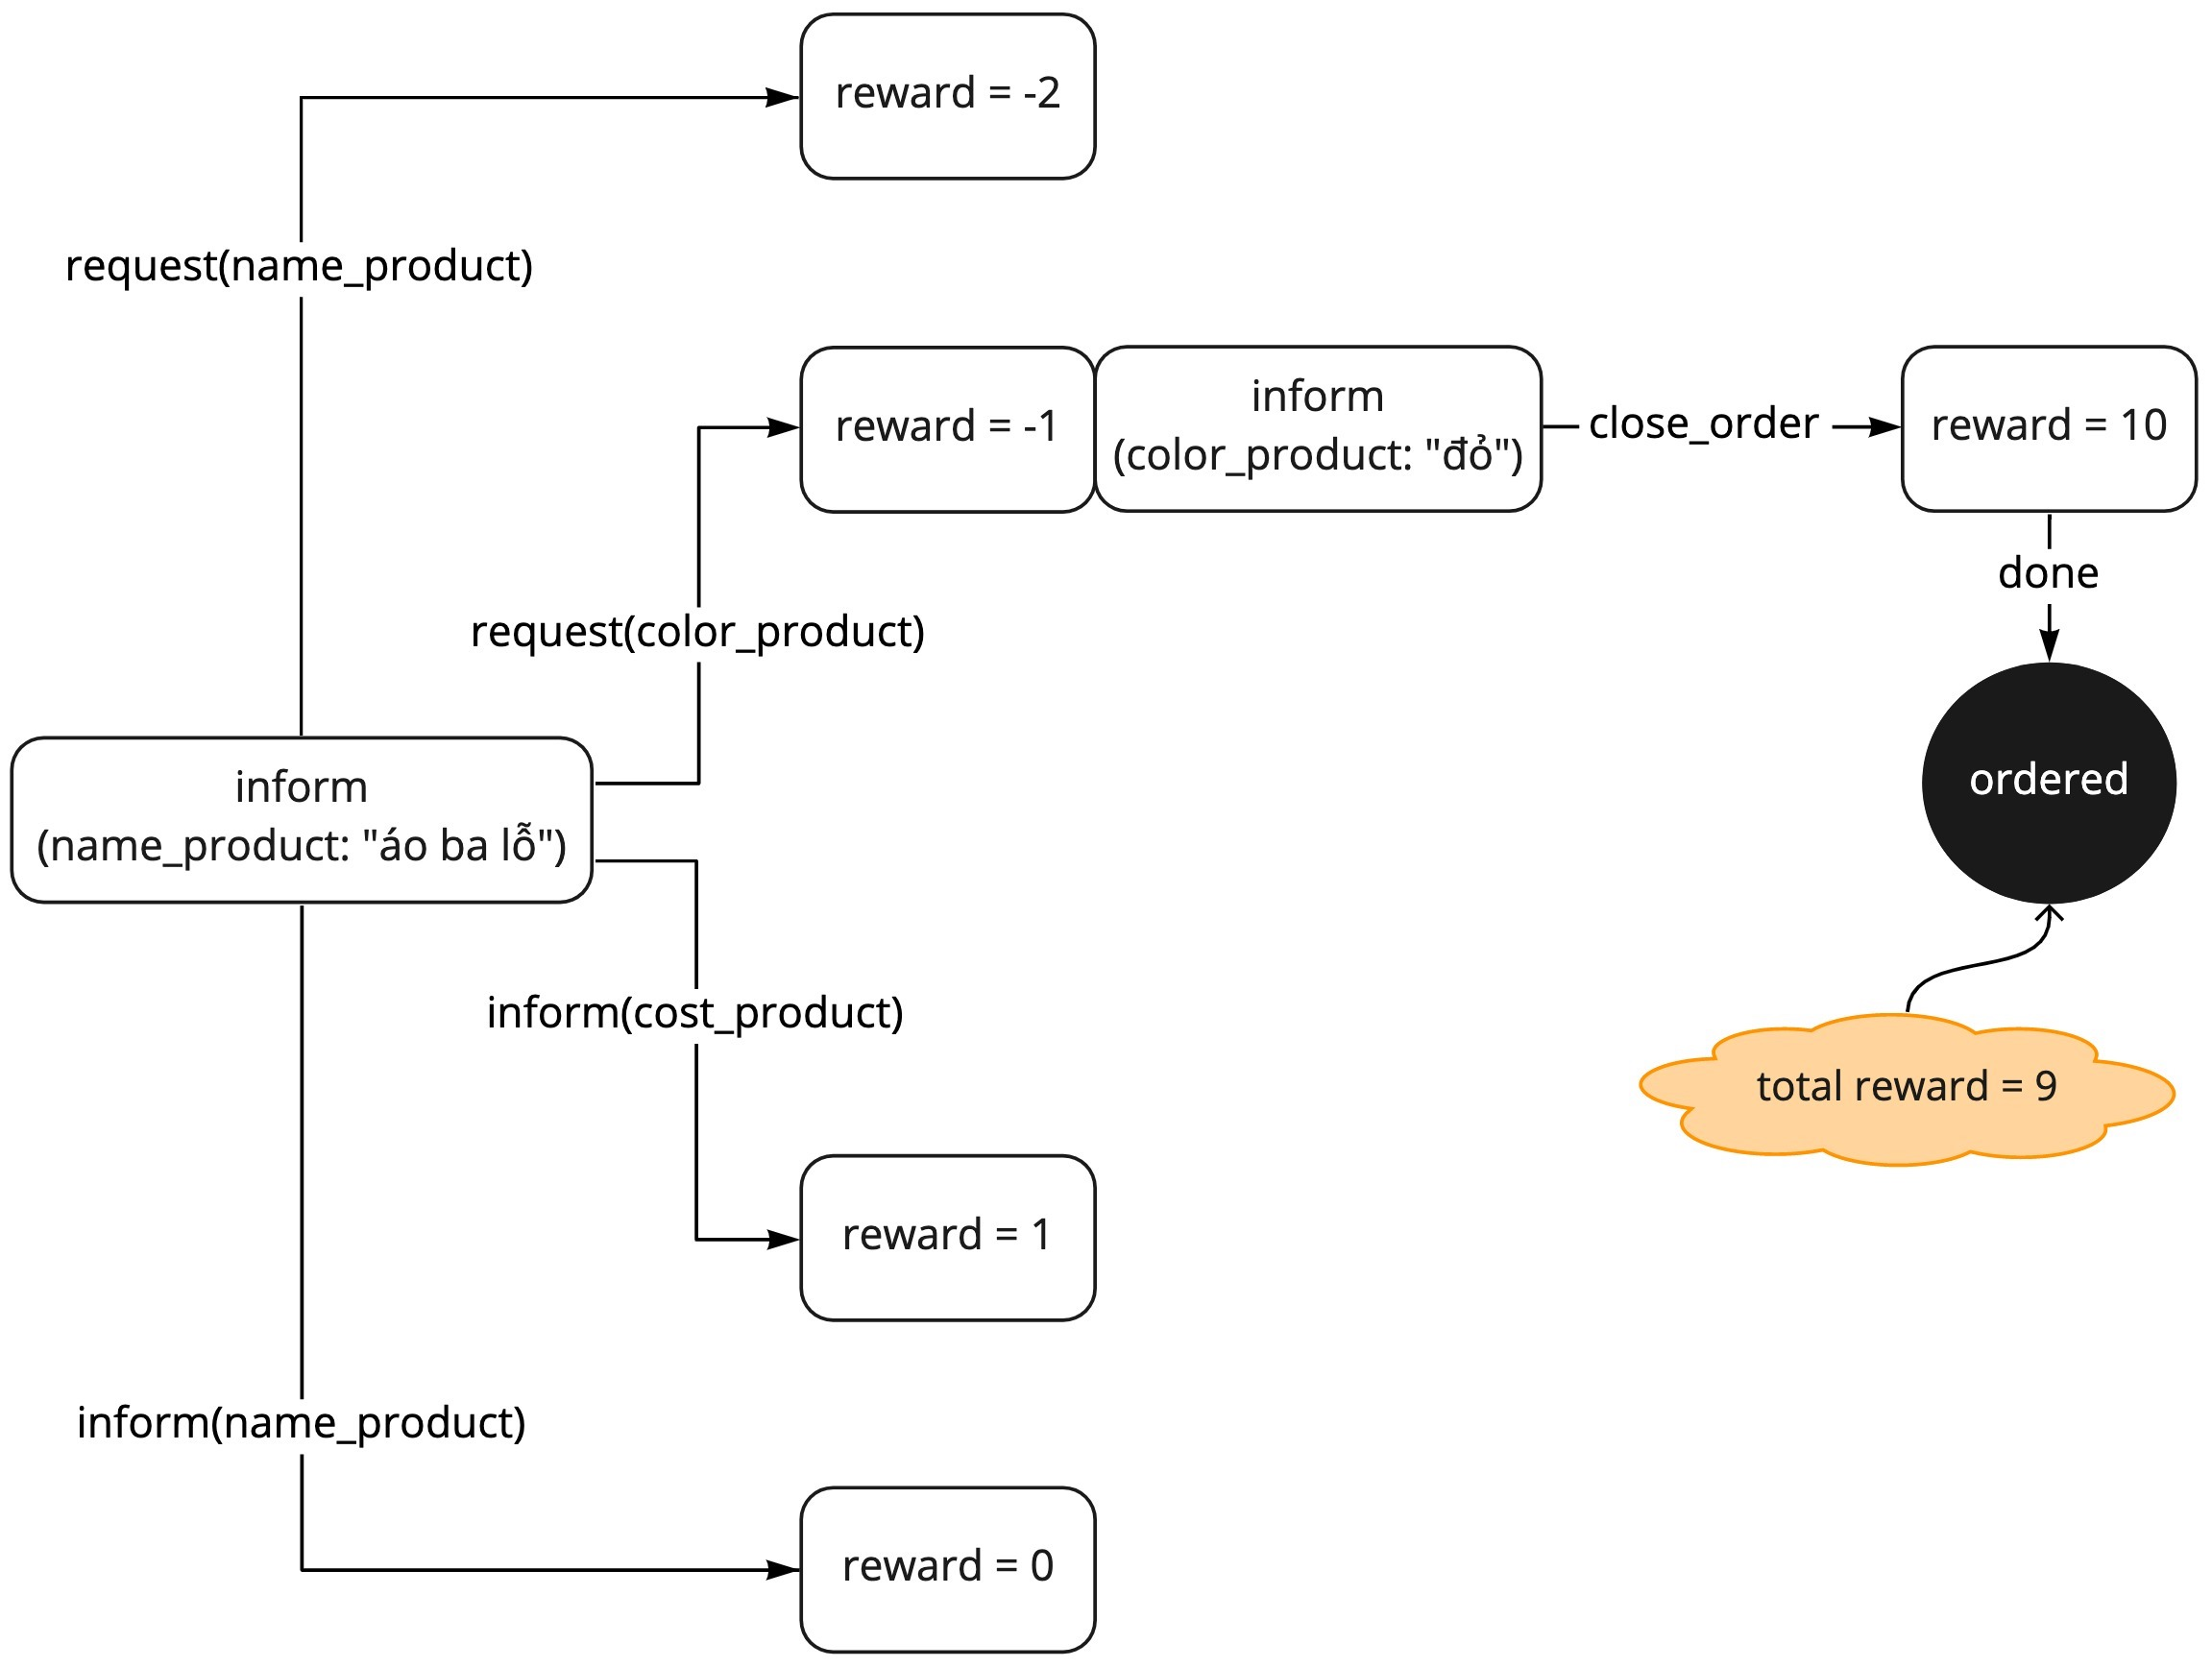
\includegraphics[scale=0.18]{thesis/chatbot/kienthuc/img/dialog_ex13.jpg}
    \caption{Quá trình cho điểm thưởng và ra hành động - phương án 1}
    \label{fig:dialog2}
\end{figure}

Ta có, quá trình một hội thoại với mục tiêu là chốt đơn hàng.
Đầu tiên, người dùng cung cấp thông tin tên sản phẩm (áo ba lỗ).
Và tác nhân có các hành động có thể có như sau:

\begin{itemize}
    \item Yêu cầu tên sản phẩm: người dùng đã cung cấp tên sản phẩm
    trước đó. Vì vậy, đây là hành vi không đúng, gây phiền nhiễu
    khó chịu cho người dùng. Nó nhận điểm trừ 2.
    \item Yêu cầu thông tin màu sắc: màu sắc là thông tin chưa được
    cung cấp, tuy nhiên đây là hành vi yêu cầu, không cung cấp
    thông tin hữu ích cho người dùng. Nó nhận điểm trừ 1.
    \item Thông báo giá sản phẩm: đây là hành vi cung cấp thông tin
    hữu ích. Nó nhận điểm thưởng 1.
    \item Thông báo tên sản phẩm: người dùng đã cung cấp tên sản phẩm
    trước đó. Vì vậy, đây là hành vi không cần thiết. Không nhận
    điểm thưởng nào.
\end{itemize}

Vì mục tiêu của hội thoại này là chốt đơn hàng. Và trong thực tế,
ta cần biết đủ thông tin sản phẩm để có được một mẫu hàng duy nhất.
Với sản phẩm này có nhiều màu, tác nhân cần yêu cầu người dùng
cung cấp thông tin màu sắc sản phẩm mà họ muốn. Sau khi có được
thông tin này, nó sẽ hoàn thành được mục tiêu hội thoại với hành động
chốt đơn hàng và nhận được điểm thưởng 10. Với luồng hội thoại này,
ta nhận được tổng phần thưởng là 9. Qua ví dụ này, ta thấy rằng để
hoàn thành được mục tiêu cuối cùng của người dùng, ngoài việc xét
điểm thưởng ở mỗi hành động, ta còn phải quan tâm đến phần thưởng
của cả cuộc hội thoại.

Xét một trường hợp khác như hình \ref{fig:dialog3}.

\begin{figure}[ht!]
    \centering
    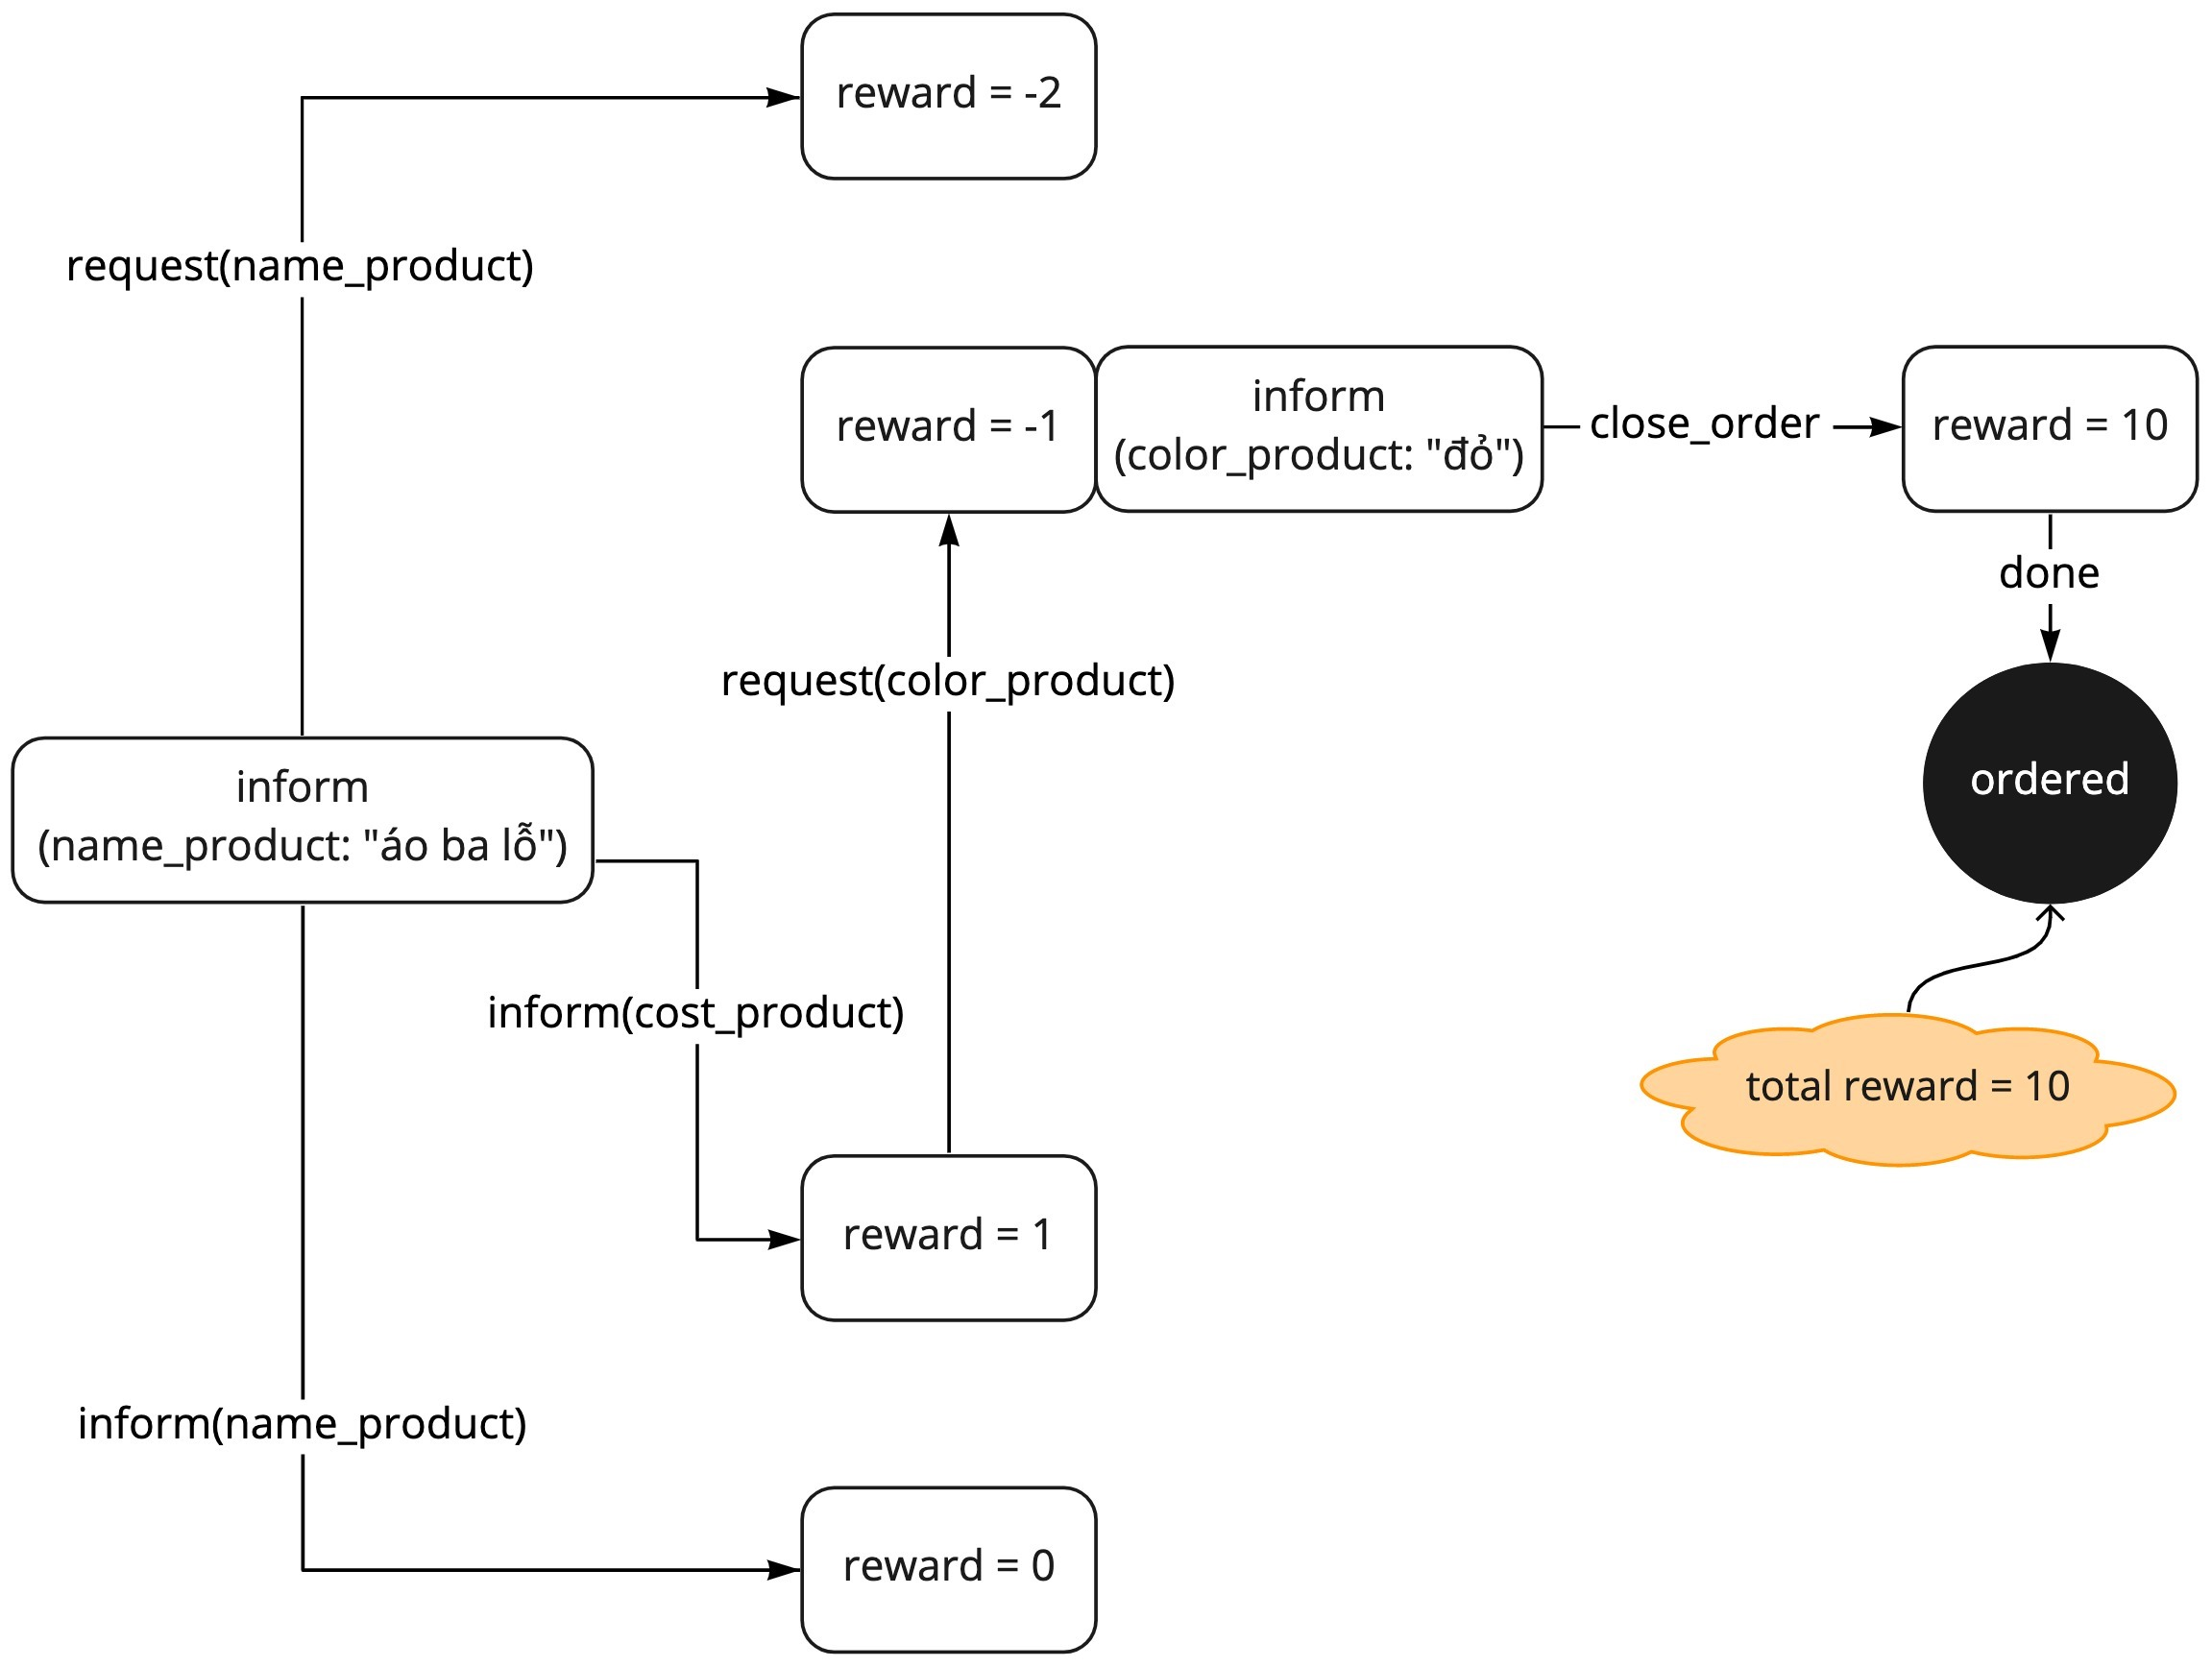
\includegraphics[scale=0.18]{thesis/chatbot/kienthuc/img/dialog_ex15.jpg}
    \caption{Quá trình cho điểm thưởng và ra hành động - phương án 2}
    \label{fig:dialog3}
\end{figure}

Thay vì ngay lập tức yêu cầu thông tin màu sắc, tác nhân có thể
thông báo một thông tin hữu ích là giá đơn hàng, nhận được
phần thưởng là 1. Mặc dù, nó không được yêu cầu bởi người dùng.
Khi đó, tổng phần thưởng nhận được có giá trị là 10, cao hơn
trường hợp lúc nãy. Tuy nhiên, như đã biết, ta mong đợi tác nhân
hoàn thành mục tiêu cho người dùng nhanh nhất có thể. Hạn chế các
hành động không cần thiết. Vì vậy, ngoài điểm thưởng cho từng
hành động, quá trình tính tổng điểm thưởng, còn kèm theo một tham số,
gọi là gamma ($\gamma$). Tham số này nhỏ hơn 1. Với mỗi điểm thưởng
cho từng hành động sẽ được nhân với lũy thừa của gamma. Với bậc là
số lượt hội thoại đã thực hiện cho đến hiện tại. Việc này sẽ làm giảm
giá trị tổng điểm thưởng khi tác nhân càng đi nhiều bước (thực hiện
nhiều hành động) trước khi đạt được mục tiêu cuối cùng. Cách tính
tổng điểm thưởng như trên, ta gọi đó là tính giá trị Q (Q-value).
Và cách học chọn hành động từ Q-value đó gọi là Q-Learning.

\subsection{Q-Learning}
Giả sử, tác nhân đang ở trạng thái $s$ và phải chọn một hành động
$a$, nó sẽ nhận được phần thưởng $r$ và đạt trạng thái mới $s'$.
Cách mà tác nhân chọn được gọi là \textit{policy}.

\begin{equation*}
    s \xrightarrow{\text{a}} r,s'
\end{equation*}

Ta định nghĩa một hàm $Q(s,a)$ sao cho khi nhận vào trạng thái $s$
và hành động $a$ nó sẽ trả về một giá trị ước lượng là tổng
phần thưởng mà ta sẽ đạt được tại trạng thái đó khi ta thực hiện
hành động $a$ và thực hiện một số \textit{policy} tiếp theo sau đó.
Ta chắc chắn rằng sẽ luôn có các \textit{policy} tối ưu, nghĩa là nó
luôn chọn được hành động tốt nhất. Ta gọi hàm $Q$ trong trường hợp
luôn có \textit{policy} tối ưu là $Q^*$. Nếu ta biết được hàm $Q^*$,
ta chỉ cần áp dụng chiến lược tham lam (greedy) lên hàm đó. Cụ thể
với mỗi trạng thái $s$, ta sẽ chọn một hành động $a$ sao cho
cực đại hoá hàm $Q^*$, hay ${max_a}{Q^*}(s,a)$. Mục tiêu của chúng ta
là tìm được hàm đủ tốt để ước lượng được hàm $Q^*$ rồi sau đó áp dụng
chiến lược tham lam lên nó. Ta viết lại hàm $Q^*$ ở dạng sau:

\begin{equation*}
    Q^*(s,a) = r_0 + {\gamma}r_1 + {\gamma}^{2}r_2 + {\gamma}^{3}r_3 + ...
\end{equation*}

Hàm $Q^*$ lúc này là tổng giá trị của phần thưởng nhận được sau mỗi
hành động tính từ hành động $a$ trở đi. $\gamma$ là giá trị khấu hao
của phần thưởng sau mỗi hành động và nó luôn nhỏ hơn 1 để
đảm bảo rằng công thức này có giới hạn. Vì có hệ số mũ nên giá trị
phần thưởng sẽ giảm dần và tiến về 0. Hệ số $\gamma$ vì vậy mà sẽ
điều khiển mức độ phụ thuộc vào tương lai của hàm $Q$ tại
trạng thái $s$.

Ta có thể viết lại hàm $Q^*$ ở trên như sau:

\begin{equation*}
    Q^*(s,a) = r_0 + {\gamma}(r_1 + {\gamma}r_2 + {\gamma}^{2}r_3 + ...) = r_0 + {\gamma}max_{a}Q^{*}(s',a)
\end{equation*}

Công thức này cho thấy giá trị hàm $Q$ của hành động $a$ tại
trạng thái $s$ bằng phần thưởng $r(s,a)$ cộng với giá trị hàm $Q$
lớn nhất của các trạng thái $s'$ tiếp theo khi thực hiện các
hành động $a$. Do đó, với công thức này chúng ta có thể tạo ra một
ma trận trạng thái-hành động (state-action) như một bảng tìm kiếm
(lookup table). Từ đó với mỗi trạng thái, tác nhân chỉ cần tìm
hành động nào có giá trị hàm $Q$ lớn nhất là xong.

Tuy nhiên, trong thực tế số lượng trạng thái rất lớn và ta không thể
nào lưu trữ toàn bộ chúng như cách ở trên được. Vì vậy ta sẽ xấp xỉ
hàm $Q$ bằng một mạng nơ-ron. Mạng nơ-ron này sẽ nhận đầu vào là một
trạng thái và nó sẽ ước lượng giá trị của hàm $Q$ cho mỗi một
hành động. Và khi ta sử dụng nhiều tầng, ta được mạng nơ-ron học sâu.

\subsection{Deep Q-Learning}
\label{subsec:deepqlearning}
Q-Learning hoạt động tốt khi chúng ta có một môi trường tương đối
đơn giản để giải quyết, nhưng khi số lượng trạng thái và hành động
chúng ta có thể thực hiện trở nên phức tạp hơn, chúng ta sử dụng
mạng nơ-ron học sâu như một công cụ xấp xỉ hàm.

Trạng thái được đưa ra làm đầu vào và giá trị Q của tất cả các
hành động của tác nhân có thể có làm đầu ra. Sự so sánh giữa
Q-learning và Deep Q-Learning được minh họa như hình
\ref{fig:dqlearning} \cite{introductiondeepqlearningpython}.

\begin{figure}[ht!]
    \centering
    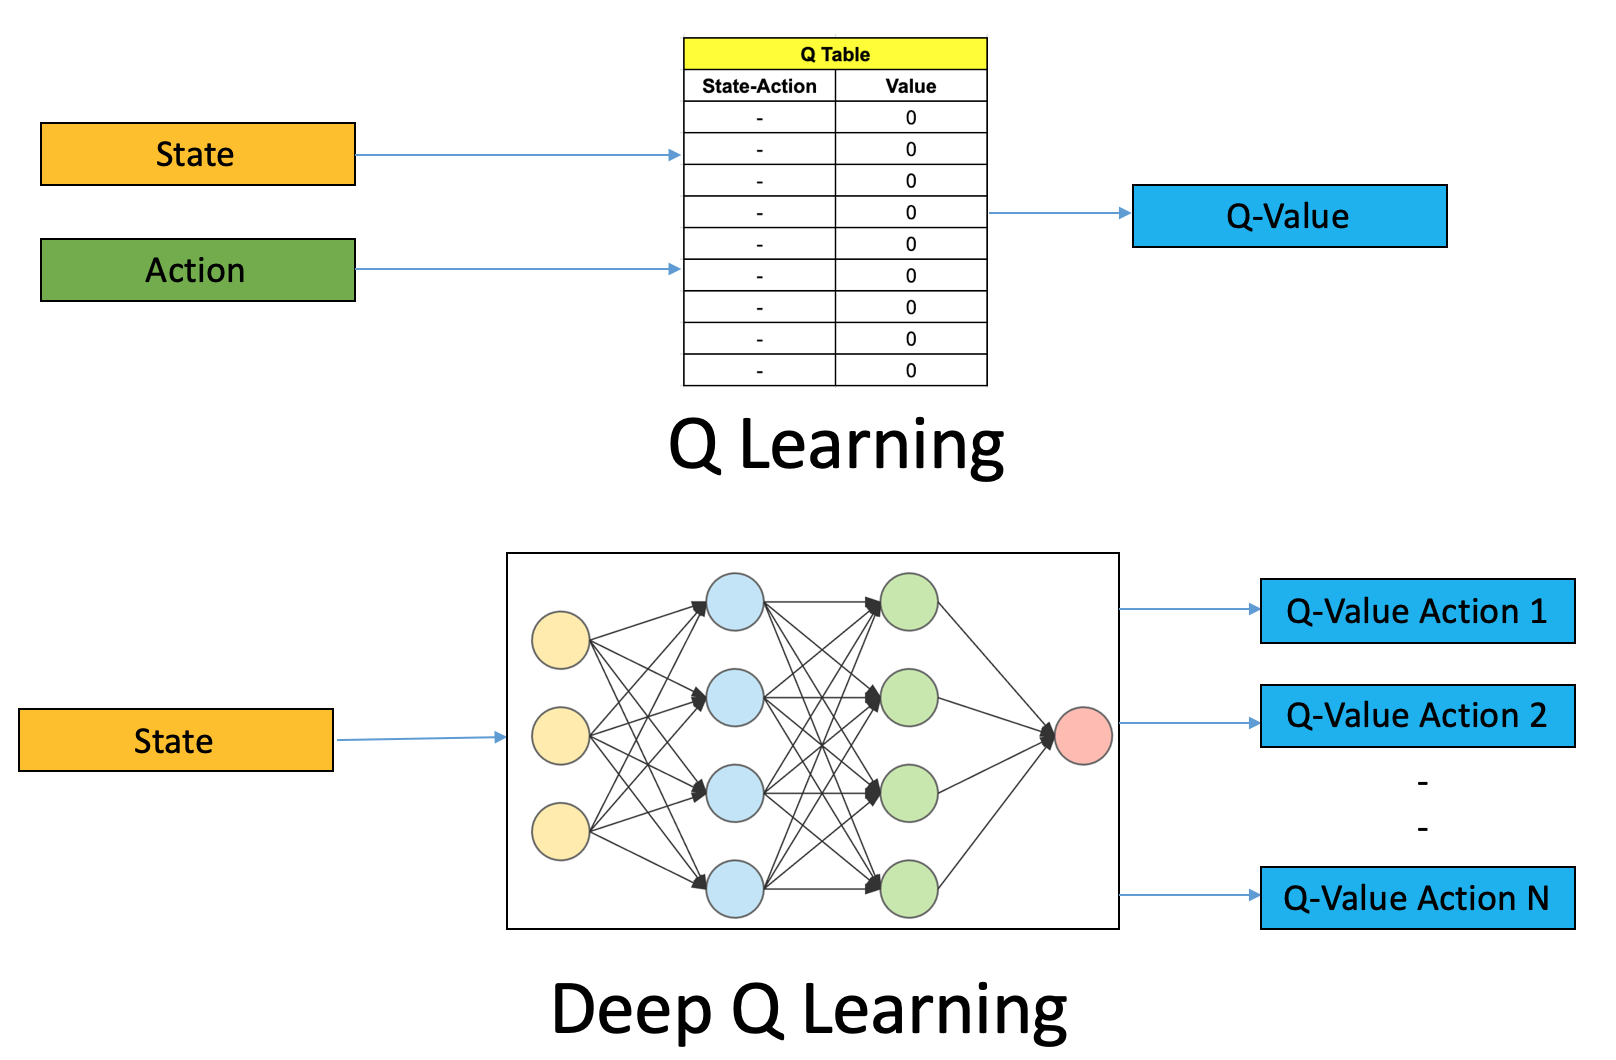
\includegraphics[scale=0.27]{thesis/chatbot/kienthuc/img/dqlearning.png}
    \caption{Q-Learning và Deep Q-Learning}
    \label{fig:dqlearning}
\end{figure}

Ta xét ví dụ sau, để làm rõ cách cập nhật trọng số của mạng nơ-ron
và chọn ra hành động.

Giả sử, trạng thái hội thoại được rút gọn lại thành chỉ chứa các
ý định hành động hiện tại của người dùng lần lượt là: hello, inform,
request, reject, done. Ta mã hóa về dạng one-hot vec-tơ để làm
đầu vào cho mạng nơ-ron. Các hành động có thể có của tác nhân là:
hello, match\_found, request, done. Mạng nơ-ron huấn luyện trong
ví dụ này như hình \ref{fig:examnetwork}. Activation của tầng ẩn là
ReLU, tầng đầu ra là linear.

\begin{figure}[ht!]
    \centering
    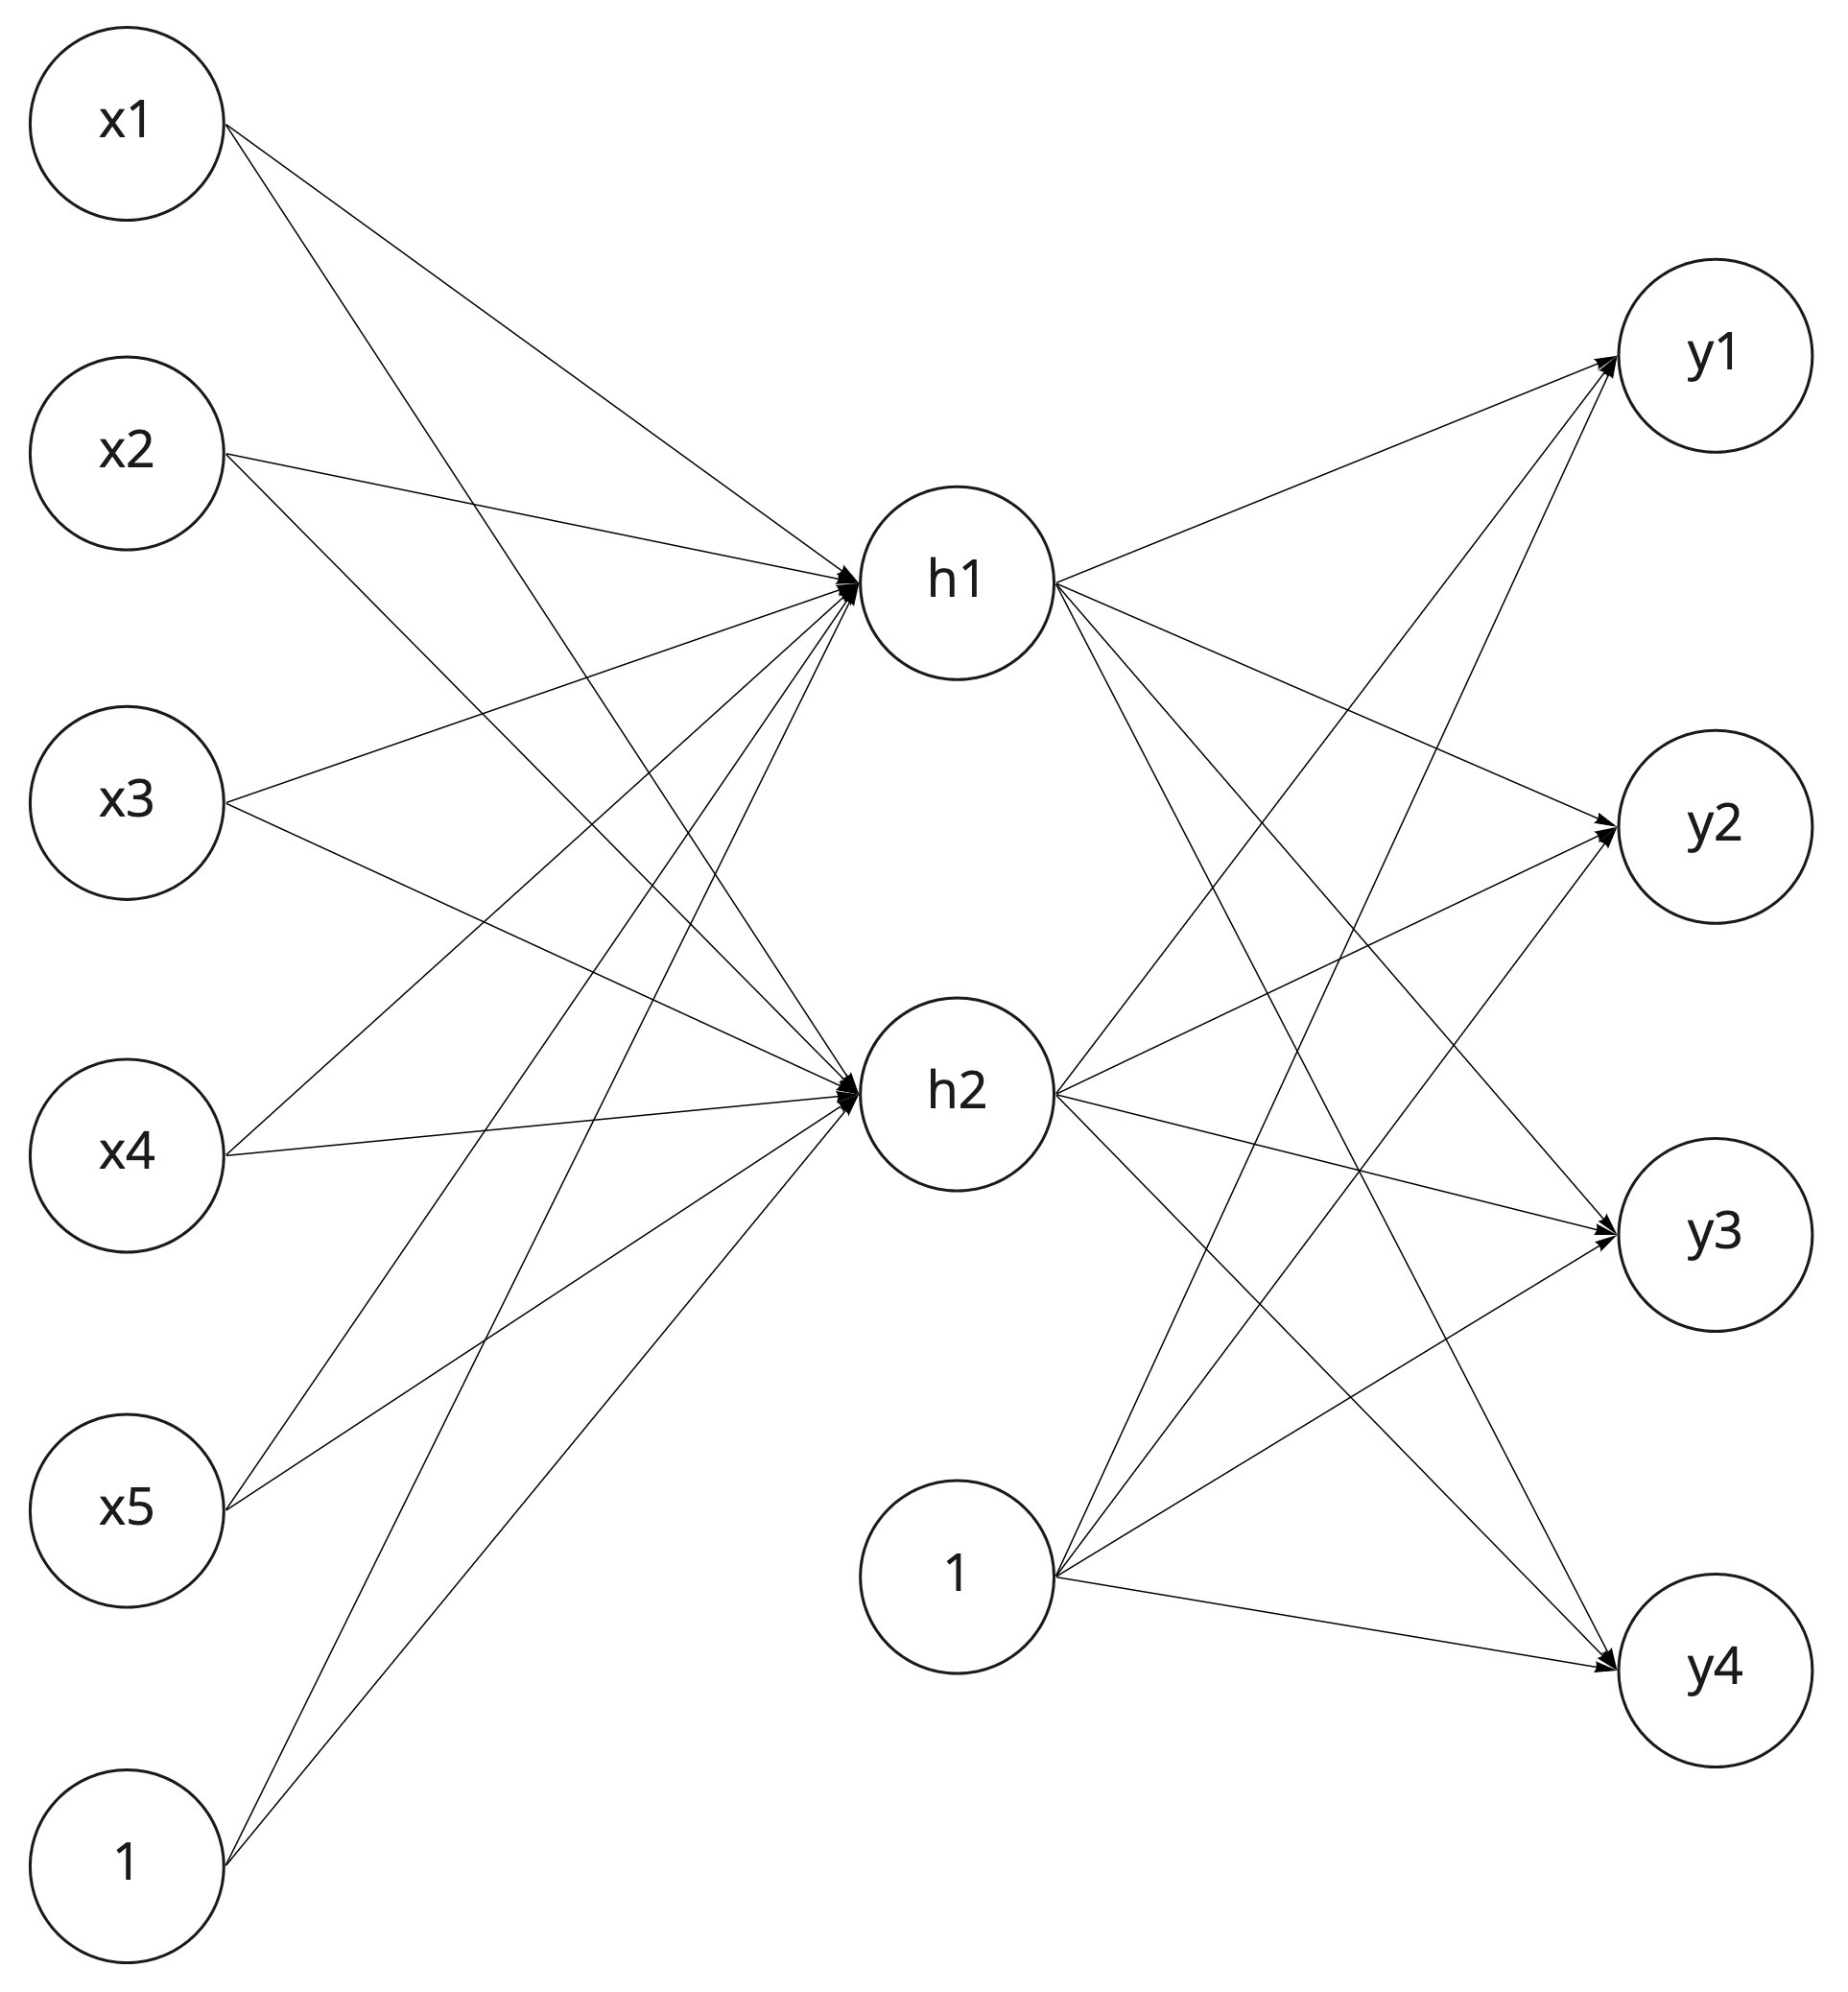
\includegraphics[scale=0.15]{thesis/chatbot/kienthuc/img/neural_network.jpg}
    \caption{Mạng nơ-ron học sâu Q-Learing}
    \label{fig:examnetwork}
\end{figure}

Giả sử, ta có ma trận trọng số cho mạng nơ-ron này như sau:

\begin{equation*}
    w_1 =
    \begin{bmatrix}
        0.18998 & 0.871522 & 0.31542 & 0.691079 & 0.902874 \\
        0.12114 & 0.84606 & 0.902874 & 0.09224 & 0.19652302
    \end{bmatrix}
\end{equation*}

\begin{equation*}
    w_2 =
    \begin{bmatrix}
        0.52141 & 0.63489 \\
        0.130012 & 0.12001 \\
        0.113114 & 0.12121 \\
        0.53514 & 0.62465
    \end{bmatrix}
\end{equation*}

\begin{equation*}
    bias = 0.325
\end{equation*}

\renewcommand{\textboxenvname}{Ví dụ}
\begin{textbox}[exam:dialog3]{Một mẫu đoạn hội thoại}
\begin{Verbatim}[breaklines=true, breakanywhere=true]
User: hello
Agent: hello
User: request
Agent: match_found
User: done
\end{Verbatim}
\end{textbox}

Sử dụng đoạn hội thoại mẫu \ref{exam:dialog3} để huấn luyện. Ta có
hành động đầu tiên của người dùng là hello. Trạng thái đầu vào $s$
như sau:

\begin{equation*}
    s =
    \begin{bmatrix}
        1 \\
        0 \\
        0 \\
        0 \\
        0
    \end{bmatrix}
\end{equation*}

Sau khi cho qua mạng nơ-ron, ta có kết quả lần lượt là:

\begin{equation*}
    w_1*s + bias =
    \begin{bmatrix}
        0.51498 \\
        0.44614
    \end{bmatrix}
\end{equation*}

\begin{equation*}
    h = relu(w_1*s + bias) =
    \begin{bmatrix}
        0.51498 \\
        0.44614
    \end{bmatrix}
\end{equation*}

\begin{equation*}
    y = h*w_2 + bias =
    \begin{bmatrix}
        0.876765546 \\
        0.445494841 \\
        0.437328077 \\
        0.879267748
    \end{bmatrix}
\end{equation*}

Kết quả ma trận y là Q-value cho từng hành động của tác nhân theo
thứ tự hello, match\_found, request, done. Với kết quả trên, ta
thấy Q-value của hành động done là lớn nhất. Dễ thấy rằng, với
hành động này, không hoàn thành được mục tiêu toàn cục. Vì vậy, ta
cần cập nhật Q-value của hành động tốt nhất tại thời điểm này.

Vì done là hành vi kết thúc hội thoại, mà hiện tại nó chưa hoàn thành
mục tiêu người dùng, nên nhận điểm trừ rất lớn là $r_0 = -10$.
Nhìn lại công thức tính $Q^*$ mục tiêu. Giả sử $\gamma = 0.9$

\begin{equation*}
    Q^*(s,a) = r_0 + {\gamma}max_{a}Q^{*}(s',a)
\end{equation*}

Để có $Q(s',a)$, ta cho đầu vào mạng nơ-ron là trạng thái kế tiếp
$s'$. Dựa vào mẫu hội thoại huấn luyện trên, ta có trạng thái
đầu vào $s'$ như sau:

\begin{equation*}
    s' =
    \begin{bmatrix}
        0 \\
        0 \\
        1 \\
        0 \\
        0
    \end{bmatrix}
\end{equation*}

Sau khi cho qua mạng nơ-ron, ta nhận được kết quả đầu ra là:

\begin{equation*}
    y =
    \begin{bmatrix}
        1.438486316 \\
        0.555619444 \\
        0.546271075 \\
        1.434705853
    \end{bmatrix}
\end{equation*}

Ta có $Q$ lớn nhất với trạng thái đầu vào $s'$ là 1.438486316.

\begin{equation*}
    => Q^*(s,a) = -10 + 0.9*1.438486316 = -8.705362316
\end{equation*}

Sau đó, mô hình sẽ được huấn luyện lại với đầu vào là trạng thái $s$
và giá trị $Q$ được cập nhật lại như sau:

\begin{equation*}
    y =
    \begin{bmatrix}
        0.876765546 \\
        0.445494841 \\
        0.437328077 \\
        -8.705362316
    \end{bmatrix}
\end{equation*}

\chapter{Mô tả hệ thống}

\section{Kiến trúc tổng quát của hệ thống}
Để giải quyết các vấn đề đã được trình bày ở mục \ref{sec:muctieu},
hệ thống ứng dụng Chatbot tư vấn có các thành phần chính đó là phần
giao diện giao tiếp với người dùng, dữ liệu thời trang phục vụ cho
việc tư vấn và phần lõi của hệ thống. Mối quan hệ giữa các thành phần
được biểu diễn như hình \ref{fig:chatbotapp}

\begin{figure}[ht!]
    \centering
    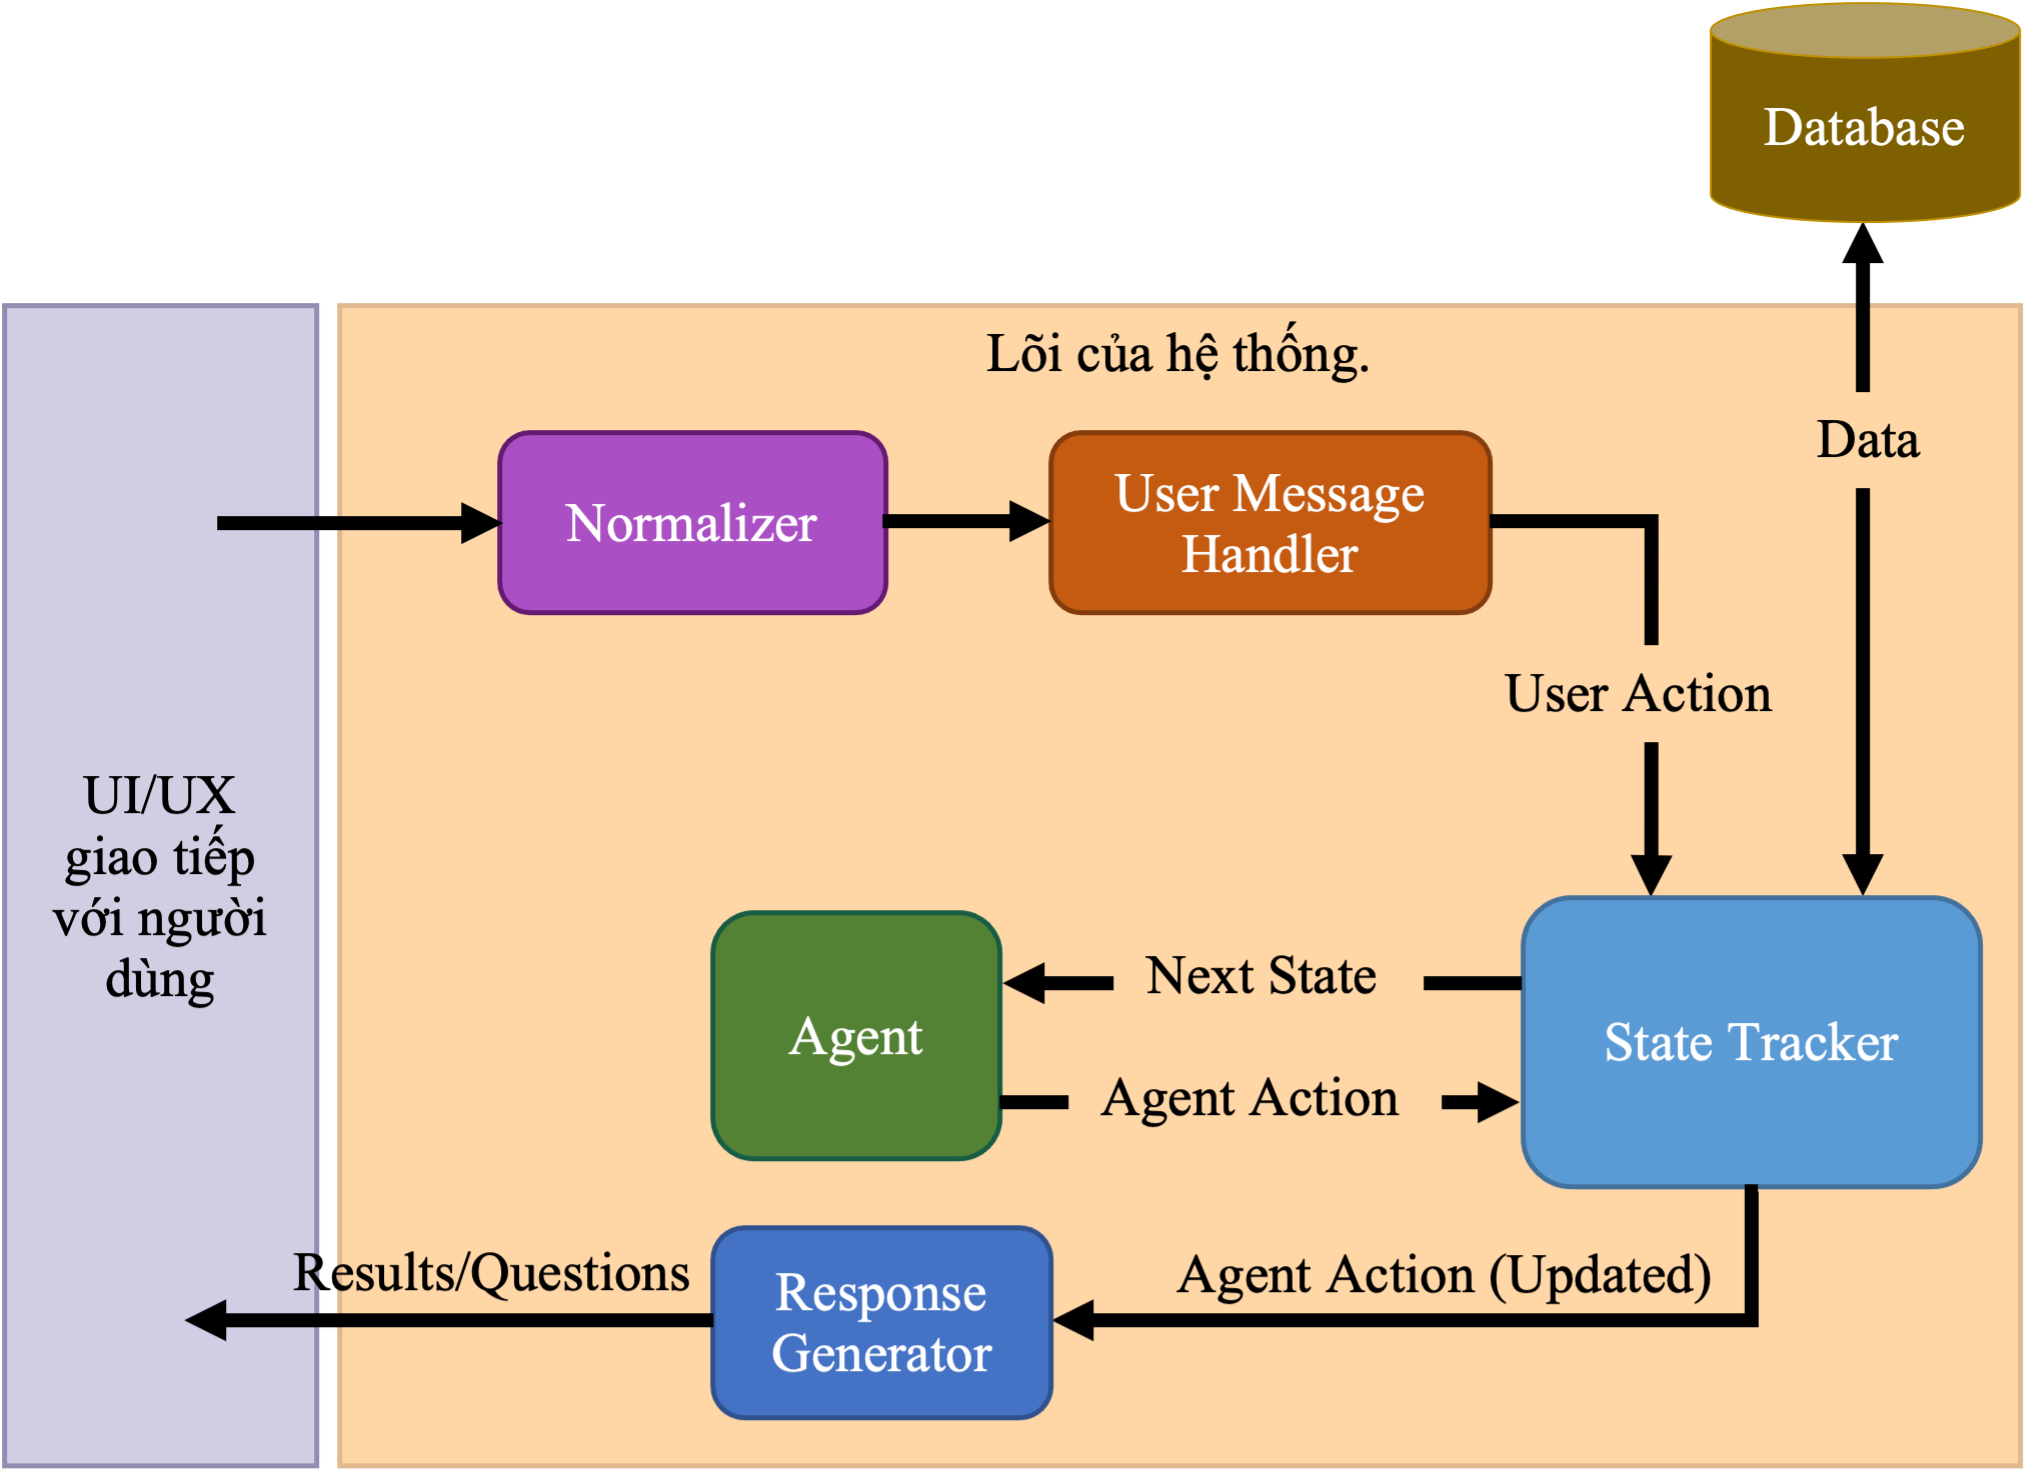
\includegraphics[scale=0.95]{thesis/chatbot/phuongphap/img/chatbot_app.png}
    \caption{Kiến trúc tổng quát của hệ thống Chatbot}
    \label{fig:chatbotapp}
\end{figure}

Trong phần lõi của hệ thống, ta có các phần con khác được mô tả
cụ thể sau đây:

\begin{itemize}
    \item \textbf{Normalizer (Bộ chuẩn hóa dữ liệu):} dữ liệu
    sau khi nhận được từ người dùng sẽ được chuẩn hóa để thống nhất
    về cách biểu diễn trước khi tạo \textit{User Action} (hành động
    của người dùng) và lưu vào cơ sở dữ liệu.
    \item \textbf{User Message Handler (Bộ xử lý phản hồi
    người dùng):} có nhiệm vụ tạo ra \textit{User Action}.
    \item \textbf{State Tracker (Bộ quản lý trạng thái hội thoại):}
    có nhiệm vụ giám sát trạng thái hiện tại của cuộc hội thoại để
    cung cấp thông tin cho \textit{agent} (tác nhân) ra quyết định,
    đồng thời thực hiện truy xuất vào cơ sở dữ liệu để lấy các
    thông tin cần thiết trước khi gửi kèm nó cùng với phản hồi
    từ \textit{agent}.
    \item \textbf{Agent (Bộ sinh phản hồi):} có nhiệm vụ dựa vào
    trạng thái hiện tại mà \textit{State Tracker} cung cấp để đưa ra
    quyết định phản hồi một hành động cụ thể và gửi về lại
    \textit{State Tracker}.
    \item \textbf{Response Generator (Bộ sinh câu phản hồi):} có
    nhiệm vụ chuyển đổi \textit{Agent Action} nhận từ
    \textit{State Tracker} tạo ra câu phản hồi dưới dạng ngôn ngữ
    tự nhiên trước khi gửi về cho người dùng.
\end{itemize}

\section{Sơ đồ tình huống sử dụng (Use Case Diagram)}

\begin{figure}[ht!]
    \centering
    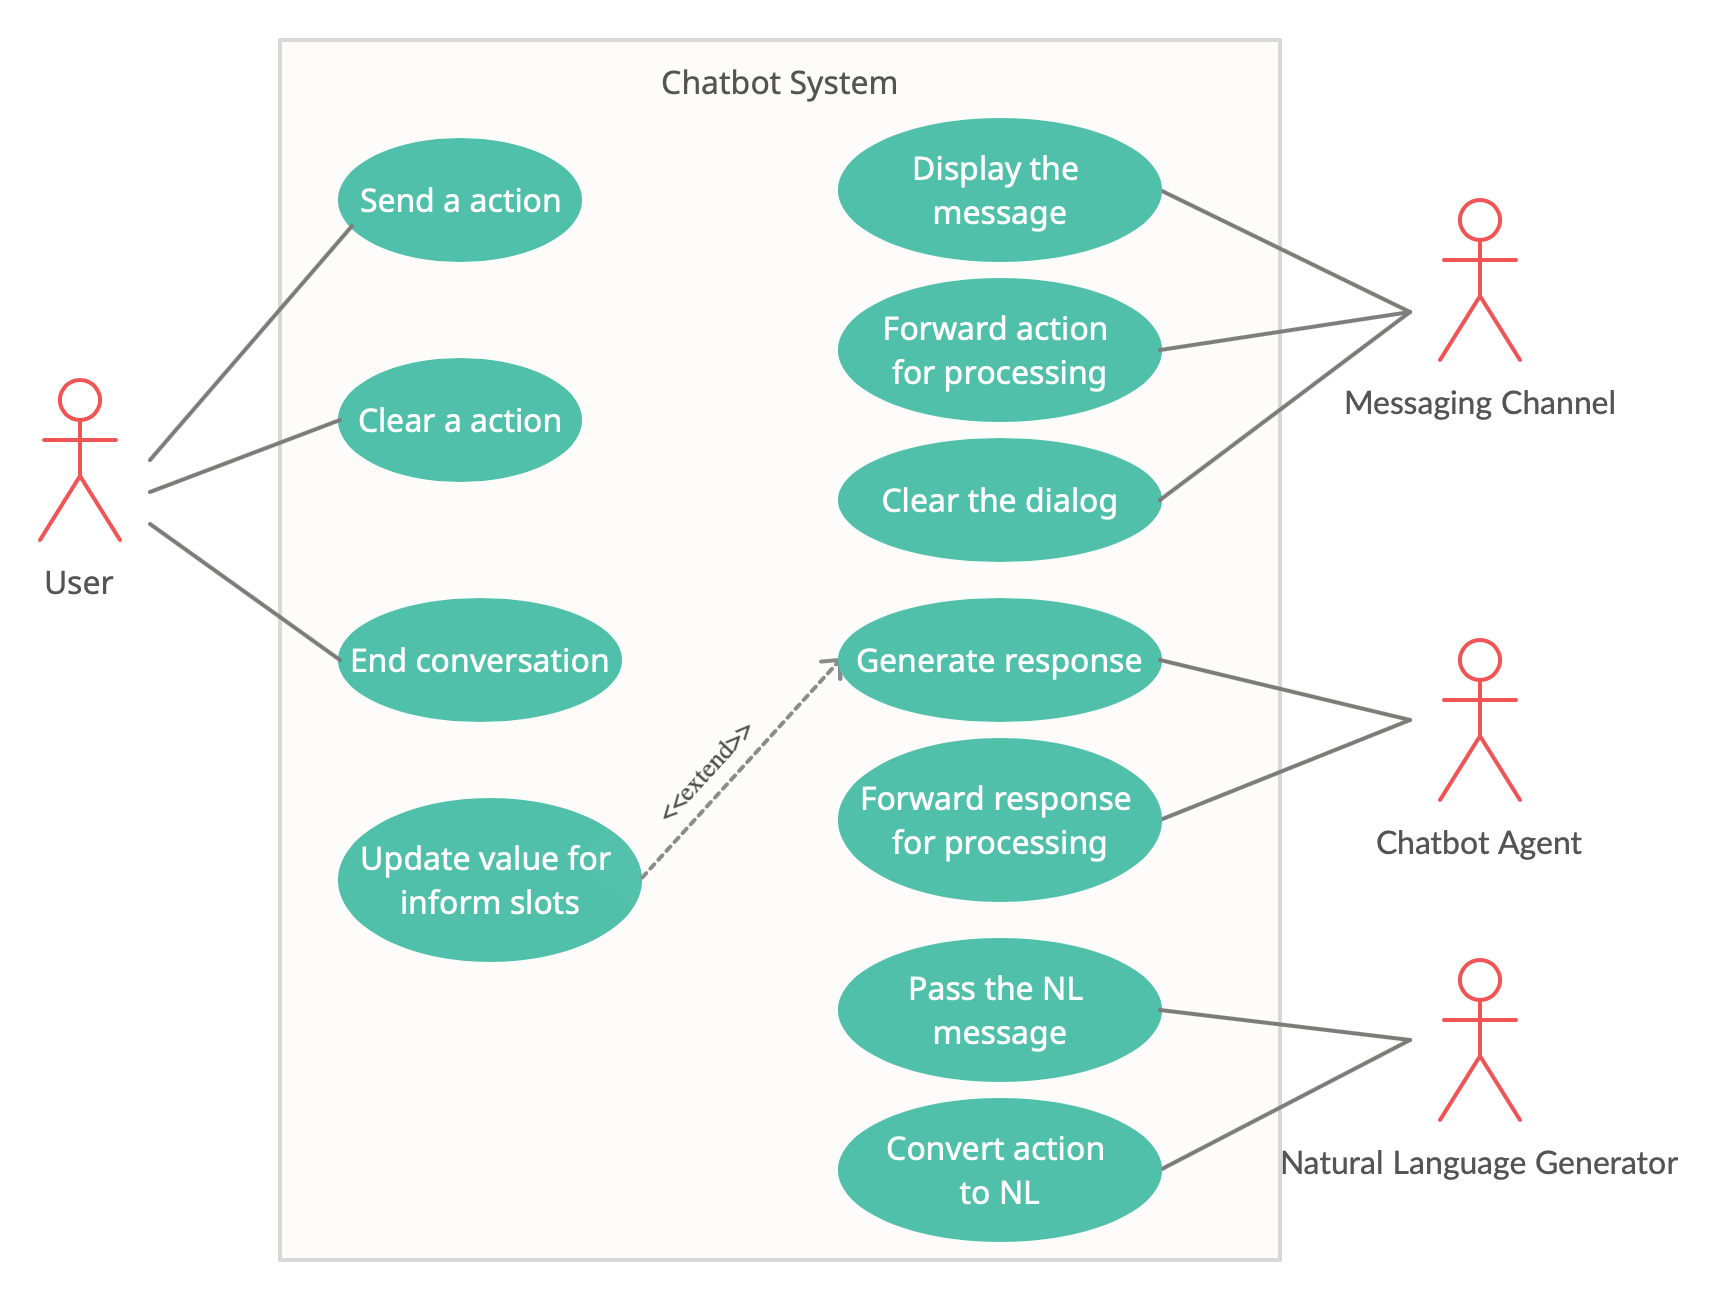
\includegraphics[scale=0.25]{thesis/chatbot/phuongphap/img/use_case.png}
    \caption{Sơ đồ tình huống sử dụng (Use Case Diagram) của hệ thống
    Chatbot}
    \label{fig:usecase}
\end{figure}

Sơ đồ tình huống sử dụng (Use Case Diagram) của hệ thống Chatbot được
diễn tả ở hình \ref{fig:usecase}. Có các thành phần cụ thể như sau:

\begin{itemize}
    \item \textbf{Actor:}
    \begin{itemize}
        \item \textbf{User:} Người dùng cuối của Chatbot. Giao tiếp
        với hệ thống thông qua giao diện Chatbot.
        \item \textbf{Messaging Channel:} Kênh thông tin liên lạc
        giữa người dùng và tác nhân.
        \item \textbf{Chatbot Agent:} Tác nhân sinh ra câu phản hồi
        cho người dùng.
        \item \textbf{Natural Language Generator:} Bộ tạo ra các câu
        phản hồi dưới dạng ngôn ngữ tự nhiên.
    \end{itemize}
    \item \textbf{Use case:}
    \begin{itemize}
        \item \textbf{Send a action:} Đối tượng thực hiện (actor) là
        \textit{User}. Đây là hành vi gửi đi một hành động có thể là
        yêu cầu, thông báo, xác nhận thông tin về sản phẩm của
        người dùng.
        \item \textbf{Clear a action:} Đối tượng thực hiện là
        \textit{User}. Xóa đi một hành động tạm thời đang thực hiện
        nhưng chưa được gửi đi.
        \item \textbf{End conversation:} Đối tượng thực hiện là
        \textit{User}. Yêu cầu kết thúc cuộc hội thoại hiện tại.
        \item \textbf{Forward action for processing:} Đối tượng
        thực hiện là \textit{Messaging Channel}. Đây là hành vi
        chuyển tiếp một hành động của người dùng sang bộ sinh
        ngôn ngữ tự nhiên.
        \item \textbf{Display the message:} Đối tượng thực hiện là
        \textit{Messaging Channel}. Hiển thị các câu thoại trên
        giao diện hội thoại.
        \item \textbf{Clear the dialog:} Đối tượng thực hiện là
        \textit{Messaging Channel}. Xóa toàn bộ lịch sử và nội dung
        cuộc hội thoại trên giao diện hội thoại.
        \item \textbf{Generate response:} Đối tượng thực hiện là
        \textit{Chatbot Agent}. \textit{Agent} dựa vào trạng thái
        hiện tại của hội thoại quyết định một hành động phản hồi.
        \item \textbf{Update value for inform slots:} Đối tượng
        thực hiện là \textit{Chatbot Agent}. Tùy vào hành động
        hiện tại của \textit{agent}, nếu có thông tin cần thông báo
        cho người dùng, nó sẽ truy vấn vào cơ sở dữ liệu tìm ra
        giá trị phù hợp cho thông tin đó.
        \item \textbf{Forward response for processing:} Đối tượng
        thực hiện là \textit{Chatbot Agent}. Đây là hành vi
        chuyển tiếp một hành động của \textit{agent} sang bộ sinh
        ngôn ngữ tự nhiên.
        \item \textbf{Convert action to NL:} Đối tượng thực hiện là
        \textit{Natural Language Generator}. Chuyển đổi hành động
        của người dùng và \textit{agent} sang ngôn ngữ tự nhiên.
        \item \textbf{Pass the NL message:} Đối tượng thực hiện là
        \textit{Natural Language Generator}. Hành động chuyển
        câu thoại sang kênh hội thoại.
    \end{itemize}
\end{itemize}

\section{Các ý định của người dùng}
Ý định người dùng là khái niệm nói về nhu cầu của người dùng thể hiện
qua câu thoại. Ý định người dùng có thể đơn giản chỉ là chào hỏi,
cảm thán hoặc yêu cầu về một thông tin thành phần nào đó của sản phẩm
như chất liệu, màu sắc, ... Trong mục này, mô tả các ý định người dùng
được định nghĩa trong đề tài.

\subsection{Chào hỏi}
\begin{itemize}
    \item \textbf{Mô tả:} Đây là ý định khi người dùng thực hiện các
    câu chào, hỏi thăm với cửa hàng (tác nhân Chatbot).
    \item \textbf{Ví dụ:}
    \begin{itemize}
        \item Hi shop nhé
        \item Chào bạn
    \end{itemize}
    \item \textbf{Phản hồi:} Tác nhân sẽ thực hiện câu chào phản hồi
    lại khách hàng.
\end{itemize}

\subsection{Kết thúc}
\begin{itemize}
    \item \textbf{Mô tả:} Đây là ý định khi người dùng muốn kết thúc
    cuộc hội thoại, thường là một câu chào tạm biệt.
    \item \textbf{Ví dụ:}
    \begin{itemize}
        \item Ok bye shop
        \item Bye shop nhé
    \end{itemize}
    \item \textbf{Phản hồi:} Tác nhân sẽ thực hiện câu tạm biệt
    phản hồi lại khách hàng.
\end{itemize}

\subsection{Cảm ơn/ Đồng tình}
\begin{itemize}
    \item \textbf{Mô tả:} Đây là ý định khi người dùng thể hiện ý
    đồng tình, hoặc cảm ơn câu phản hồi của tác nhân.
    \item \textbf{Ví dụ:}
    \begin{itemize}
        \item Ok shop
        \item Cảm ơn bạn
    \end{itemize}
    \item \textbf{Phản hồi:} Sau khi nhận được ý định này từ
    khách hàng, tác nhân cập nhật thông tin vào hệ thống và tiếp tục
    tiến trình cuộc hội thoại.
\end{itemize}

\subsection{Phản đối}
\begin{itemize}
    \item \textbf{Mô tả:} Đây là ý định khi người dùng thể hiện ý
    không đồng tình, phản đối câu phản hồi của tác nhân.
    \item \textbf{Ví dụ:}
    \begin{itemize}
        \item Không phải shop ạ
        \item Mình không cần
    \end{itemize}
    \item \textbf{Phản hồi:} Sau khi nhận được ý định này từ
    khách hàng, tác nhân cập nhật thông tin vào hệ thống và
    tiếp tục tiến trình cuộc hội thoại.
\end{itemize}

\subsection{Yêu cầu thông tin màu sắc}
\begin{itemize}
    \item \textbf{Mô tả:} Mỗi mẫu sản phẩm có nhiều màu khác nhau,
    phù hợp cho nhiều sở thích của khách hàng. Đây là ý định
    phát sinh khi khách hàng đặt câu hỏi với mục đích muốn có
    thông tin về các màu của sản phẩm.
    \item \textbf{Ví dụ:}
    \begin{itemize}
        \item Áo hoa này có những màu gì vậy ạ?
        \item Cho mình xin các màu của sản phẩm này
    \end{itemize}
    \item \textbf{Phản hồi:} Sau khi thu thập đủ các thông tin,
    phản hồi trả về cho khách hàng sẽ là thông tin màu sắc của
    sản phẩm có thể có, những sản phẩm này phải thỏa các điều kiện
    ràng buộc tìm được trong cơ sở dữ liệu.
\end{itemize}

\subsection{Yêu cầu thông tin chất liệu}
\begin{itemize}
    \item \textbf{Mô tả:} Mỗi mẫu sản phẩm có thể được làm bởi mỗi
    loại vật liệu khác nhau, phù hợp cho nhu cầu của khách hàng.
    Đây là ý định phát sinh khi khách hàng đặt câu hỏi với mục đích
    muốn có thông tin về chất liệu của sản phẩm.
    \item \textbf{Ví dụ:}
    \begin{itemize}
        \item Chất vải là gì vậy ạ?
        \item Đầm này vải gì vậy shop?
    \end{itemize}
    \item \textbf{Phản hồi:} Sau khi thu thập đủ các thông tin,
    phản hồi trả về cho khách hàng sẽ là thông tin chất liệu của
    sản phẩm, những sản phẩm này phải thỏa các điều kiện ràng buộc
    tìm được trong cơ sở dữ liệu.
\end{itemize}

\subsection{Yêu cầu thông tin giá bán}
\begin{itemize}
    \item \textbf{Mô tả:} Mỗi mẫu sản phẩm có thể được bán với các
    giá khác nhau, tùy vào chất liệu, màu sắc và các chi phí
    phát sinh khác. Đây là ý định phát sinh khi khách hàng đặt
    câu hỏi với mục đích muốn có thông tin về giá bán của sản phẩm.
    \item \textbf{Ví dụ:}
    \begin{itemize}
        \item Nguyên bộ này hết nhiêu tiền?
        \item Áo thun này bao tiền vậy
    \end{itemize}
    \item \textbf{Phản hồi:} Sau khi thu thập đủ các thông tin,
    phản hồi trả về cho khách hàng sẽ là thông tin giá bán có thể có
    của sản phẩm, những sản phẩm này phải thỏa các điều kiện
    ràng buộc tìm được trong cơ sở dữ liệu.
\end{itemize}

\subsection{Yêu cầu thông tin tình trạng sản phẩm}
\begin{itemize}
    \item \textbf{Mô tả:} Tại mỗi thời điểm, cửa hàng có thể có những
    mẫu sản phẩm khác nhau. Việc một số sản phẩm có thể không còn
    hoặc tạm hết trong kho của cửa hàng. Đây là ý định phát sinh khi
    khách hàng đặt câu hỏi với mục đích muốn xác nhận rằng sản phẩm
    vẫn còn được bán bởi cửa hàng.
    \item \textbf{Ví dụ:}
    \begin{itemize}
        \item Đầm caro còn không shop
        \item Áo này còn màu xanh không?
    \end{itemize}
    \item \textbf{Phản hồi:} Sau khi thu thập đủ các thông tin,
    phản hồi trả về cho khách hàng sẽ là thông tin hiện tại của
    sản phẩm, những sản phẩm này phải thỏa các điều kiện ràng buộc
    tìm được trong cơ sở dữ liệu.
\end{itemize}

\subsection{Thông báo về tên sản phẩm}
\begin{itemize}
    \item \textbf{Mô tả:} Tên sản phẩm là thông tin quan trọng nhất
    trong hoạt động tư vấn. Khi bắt đầu cuộc hội thoại tư vấn,
    khách hàng sẽ có mục tiêu tư vấn cho một sản phẩm nhất định.
    Đây là ý định phát sinh khi khách hàng thông báo cho shop về
    sản phẩm mình muốn tìm hiểu.
    \item \textbf{Ví dụ:}
    \begin{itemize}
        \item Bộ set vest cổ xéo shop ơi.
        \item Mình muốn tư vấn đầm hoa này ạ
    \end{itemize}
    \item \textbf{Phản hồi:} Sau khi nhận được ý định này từ
    khách hàng, tác nhân cập nhật thông tin vào hệ thống và
    tiếp tục tiến trình cuộc hội thoại.
\end{itemize}

\subsection{Thông báo về màu sắc}
\begin{itemize}
    \item \textbf{Mô tả:} Sau khi có được các thông tin về sản phẩm
    mong muốn của khách hàng. Họ có thể sẽ muốn đặt mua một sản phẩm
    có màu cụ thể như yêu cầu. Đây là ý định phát sinh khi khách hàng
    muốn đặt mua sản phẩm và thông báo cho shop về màu sắc của
    sản phẩm cần lấy.
    \item \textbf{Ví dụ:}
    \begin{itemize}
        \item Mình lấy cái màu đen này nha.
        \item Cái set vest này mình lấy màu trắng.
    \end{itemize}
    \item \textbf{Phản hồi:} Sau khi thu thập đủ các thông tin,
    phản hồi trả về cho khách hàng sẽ là toàn bộ thông tin về
    sản phẩm mà khách hàng đã đặt, những sản phẩm này phải thỏa
    các điều kiện ràng buộc tìm được trong cơ sở dữ liệu.
\end{itemize}

\subsection{Thông báo về kích cỡ}
\begin{itemize}
    \item \textbf{Mô tả:} Sau khi có được các thông tin về sản phẩm
    mong muốn của khách hàng. Họ có thể sẽ muốn đặt mua một sản phẩm
    có kích cỡ cụ thể như yêu cầu. Đây là ý định phát sinh khi
    khách hàng muốn đặt mua sản phẩm và thông báo cho shop về
    kích cỡ của sản phẩm cần lấy.
    \item \textbf{Ví dụ:}
    \begin{itemize}
        \item Cho mình đặt 1 áo hoa size S ạ
        \item Bộ này mình lấy size S ạ.
    \end{itemize}
    \item \textbf{Phản hồi:} Sau khi thu thập đủ các thông tin,
    phản hồi trả về cho khách hàng sẽ là toàn bộ thông tin về
    sản phẩm mà khách hàng đã đặt, những sản phẩm này phải thỏa
    các điều kiện ràng buộc tìm được trong cơ sở dữ liệu.
\end{itemize}

\subsection{Thông báo về số lượng}
\begin{itemize}
    \item \textbf{Mô tả:} Sau khi có được các thông tin về sản phẩm
    mong muốn của khách hàng. Họ có thể sẽ muốn đặt mua một số lượng
    sản phẩm. Đây là ý định phát sinh khi khách hàng muốn đặt mua
    sản phẩm và thông báo cho shop về số lượng sản phẩm cần lấy.
    \item \textbf{Ví dụ:}
    \begin{itemize}
        \item Mình lấy 2 bộ này nha
        \item Cho mình đặt 2 cái áo hoa ạ.
    \end{itemize}
    \item \textbf{Phản hồi:} Sau khi thu thập đủ các thông tin,
    phản hồi trả về cho khách hàng sẽ là toàn bộ thông tin về
    sản phẩm mà khách hàng đã đặt, những sản phẩm này phải thỏa
    các điều kiện ràng buộc tìm được trong cơ sở dữ liệu.
\end{itemize}

\subsection{Yêu cầu tên sản phẩm}
\begin{itemize}
    \item \textbf{Mô tả:} Tên sản phẩm là thông tin quan trọng nhất
    trong hoạt động tư vấn. Đôi khi khách hàng không có nhu cầu
    bắt buộc phải tư vấn cho một sản phẩm cụ thể. Đây là ý định
    phát sinh khi khách hàng muốn tìm kiếm một sản phẩm nào đó
    trong cửa hàng mà thỏa mãn các điều kiện khác của khách hàng.
    \item \textbf{Ví dụ:}
    \begin{itemize}
        \item Có cái nào màu xanh không shop?
    \end{itemize}
    \item \textbf{Phản hồi:} Sau khi thu thập đủ các thông tin,
    phản hồi trả về cho khách hàng sẽ là tên của các sản phẩm phù hợp
    với nhu cầu của khách hàng, những sản phẩm này phải thỏa các
    điều kiện ràng buộc tìm được trong cơ sở dữ liệu.
\end{itemize}

\subsection{Yêu cầu thông tin kích cỡ}
\begin{itemize}
    \item \textbf{Mô tả:} Mỗi mẫu sản phẩm sẽ có các kích cỡ
    khác nhau, phù hợp cho nhiều thể trạng của các khách hàng.
    Đây là ý định phát sinh khi khách hàng đặt câu hỏi với
    mục đích muốn có thông tin về các loại kích cỡ của sản phẩm.
    \item \textbf{Ví dụ:}
    \begin{itemize}
        \item Có size gì ạ?
        \item Đầm này có size XS không ạ?
    \end{itemize}
    \item \textbf{Phản hồi:} Sau khi thu thập đủ các thông tin,
    phản hồi trả về cho khách hàng sẽ là kích cỡ có thể có của
    sản phẩm, những sản phẩm này phải thỏa các điều kiện
    ràng buộc tìm được trong cơ sở dữ liệu.
\end{itemize}

\subsection{Thông báo về chiều cao}
\begin{itemize}
    \item \textbf{Mô tả:} Để hổ trợ cho việc tư vấn kích cỡ phù hợp
    cho khách hàng. Đôi khi khách hàng cần cung cấp một số các
    thông tin về thể trạng cho tác nhân. Đây là ý định phát sinh khi
    khách hàng cần thông báo cho tác nhân về chiều cao của bản thân.
    \item \textbf{Ví dụ:}
    \begin{itemize}
        \item Mình cao 1m8 ạ
    \end{itemize}
    \item \textbf{Phản hồi:} Sau khi nhận được ý định này từ
    khách hàng, tác nhân cập nhật thông tin vào hệ thống và
    tiếp tục tiến trình cuộc hội thoại.
\end{itemize}

\subsection{Thông báo về cân nặng}
\begin{itemize}
    \item \textbf{Mô tả:} Để hổ trợ cho việc tư vấn kích cỡ phù hợp
    cho khách hàng. Đôi khi khách hàng cần cung cấp một số các
    thông tin về thể trạng cho tác nhân. Đây là ý định phát sinh khi
    khách hàng cần thông báo cho tác nhân về cân nặng của bản thân.
    \item \textbf{Ví dụ:}
    \begin{itemize}
        \item Nặng 46kg shop ạ
    \end{itemize}
    \item \textbf{Phản hồi:} Sau khi nhận được ý định này từ
    khách hàng, tác nhân cập nhật thông tin vào hệ thống và
    tiếp tục tiến trình cuộc hội thoại.
\end{itemize}

\subsection{Thông báo về số đo vòng eo}
\begin{itemize}
    \item \textbf{Mô tả:} Để hổ trợ cho việc tư vấn kích cỡ phù hợp
    cho khách hàng. Đôi khi khách hàng cần cung cấp một số các
    thông tin về thể trạng cho tác nhân. Đây là ý định phát sinh
    khi khách hàng cần thông báo cho tác nhân về số đo vòng eo
    của bản thân.
    \item \textbf{Ví dụ:}
    \begin{itemize}
        \item Eo mình 60 nha
    \end{itemize}
    \item \textbf{Phản hồi:} Sau khi nhận được ý định này từ
    khách hàng, tác nhân cập nhật thông tin vào hệ thống và
    tiếp tục tiến trình cuộc hội thoại.
\end{itemize}

\subsection{Bất kì (Anything)}
\begin{itemize}
    \item \textbf{Mô tả:} Khách hàng cung cấp cho tác nhân biết loại
    thông tin mà khách hàng cung cấp là không có ràng buộc.
    \item \textbf{Ví dụ:}
    \begin{itemize}
        \item Cái nào cũng được shop ạ
        \item Mình lấy màu gì cũng đc
    \end{itemize}
    \item \textbf{Phản hồi:} Sau khi nhận được ý định này từ
    khách hàng, tác nhân cập nhật thông tin vào hệ thống và
    tiếp tục tiến trình cuộc hội thoại.
\end{itemize}

\subsection{Khác (Other)}
\begin{itemize}
    \item \textbf{Mô tả:} Đây là các ý định khi khách hàng đề cập
    nội dung không liên quan tới phương diện tư vấn sản phẩm hoặc
    các thông tin chưa được định nghĩa trong hệ thống.
    \item \textbf{Ví dụ:}
    \begin{itemize}
        \item Hôm nay trời đẹp ghê.
        \item Mình cần đầm đi dạ hội.
    \end{itemize}
    \item \textbf{Phản hồi:} Sau khi nhận được ý định này từ
    khách hàng, tác nhân phản hồi theo hướng không hỗ trợ cho
    nhu cầu này của khách hàng.
\end{itemize}

\section{Kiến trúc tổng quát của mô hình huấn luyện}
\label{sec:trainingmodel}
Trong hệ thống ứng dụng Chatbot tư vấn, thành phần quan trọng nhất
là tác nhân. Trong đề tài này, sẽ thực hiện phần huấn luyện cho
tác nhân sử dụng phương pháp học tăng cường với mô hình Deep
Q-Learning như được mô tả ở mục \ref{sec:model} và áp dụng kiến trúc
trong bài hướng dẫn \cite{traininggochatbot}, cũng như sẽ có một số
điều chỉnh để phù hợp với dữ liệu và yêu cầu của hệ thống sao cho
đáp ứng được lĩnh vực đang thực hiện.

Quá trình huấn luyện được chia thành hai giai đoạn: warm-up stage
và training stage.

\subsection{Giai đoạn khởi động (Warm-up stage)}
\subsubsection{Mục tiêu}
Giai đoạn khởi động được thực hiện với mục đích tạo cho tác nhân một
ký ức (kinh nghiệm) ban đầu, thay vì cho tác nhân thực hiện các
hành động ngẫu nhiên. Quá trình này sẽ giảm thiểu được thời gian
và công sức cho việc huấn luyện sau này của tác nhân.

Có 2 cách để thực hiện quá trình trên:
\begin{itemize}
    \item Cho tác nhân lần lượt thực hiện các hành động trong một
    danh sách cố định. Mục đích cho tác nhân nhớ được tất cả các
    yêu cầu cần thiết trước khi hoàn thành mục tiêu cuối cùng
    của người dùng.
    \item Tạo ra hàng loạt các cuộc hội thoại đã được định nghĩa
    theo luật cụ thể. Các kịch bản này đều dựa trên các cuộc
    hội thoại thu thập được từ thực tế. Mục đích cho tác nhân
    có thể ra được quyết định đúng trong một trường hợp
    nhất định cụ thể và thường gặp.
\end{itemize}

\subsubsection{Các cuộc hội thoại (Dialogs)}
\label{subsubsec:dialog}
Các cuộc hội thoại (dialogs) được tạo ra dựa trên các luật đã được
định nghĩa sẵn. Hình \ref{fig:dialog} biểu diễn tổng quát
của một luật hội thoại.

\begin{figure}[ht!]
    \centering
    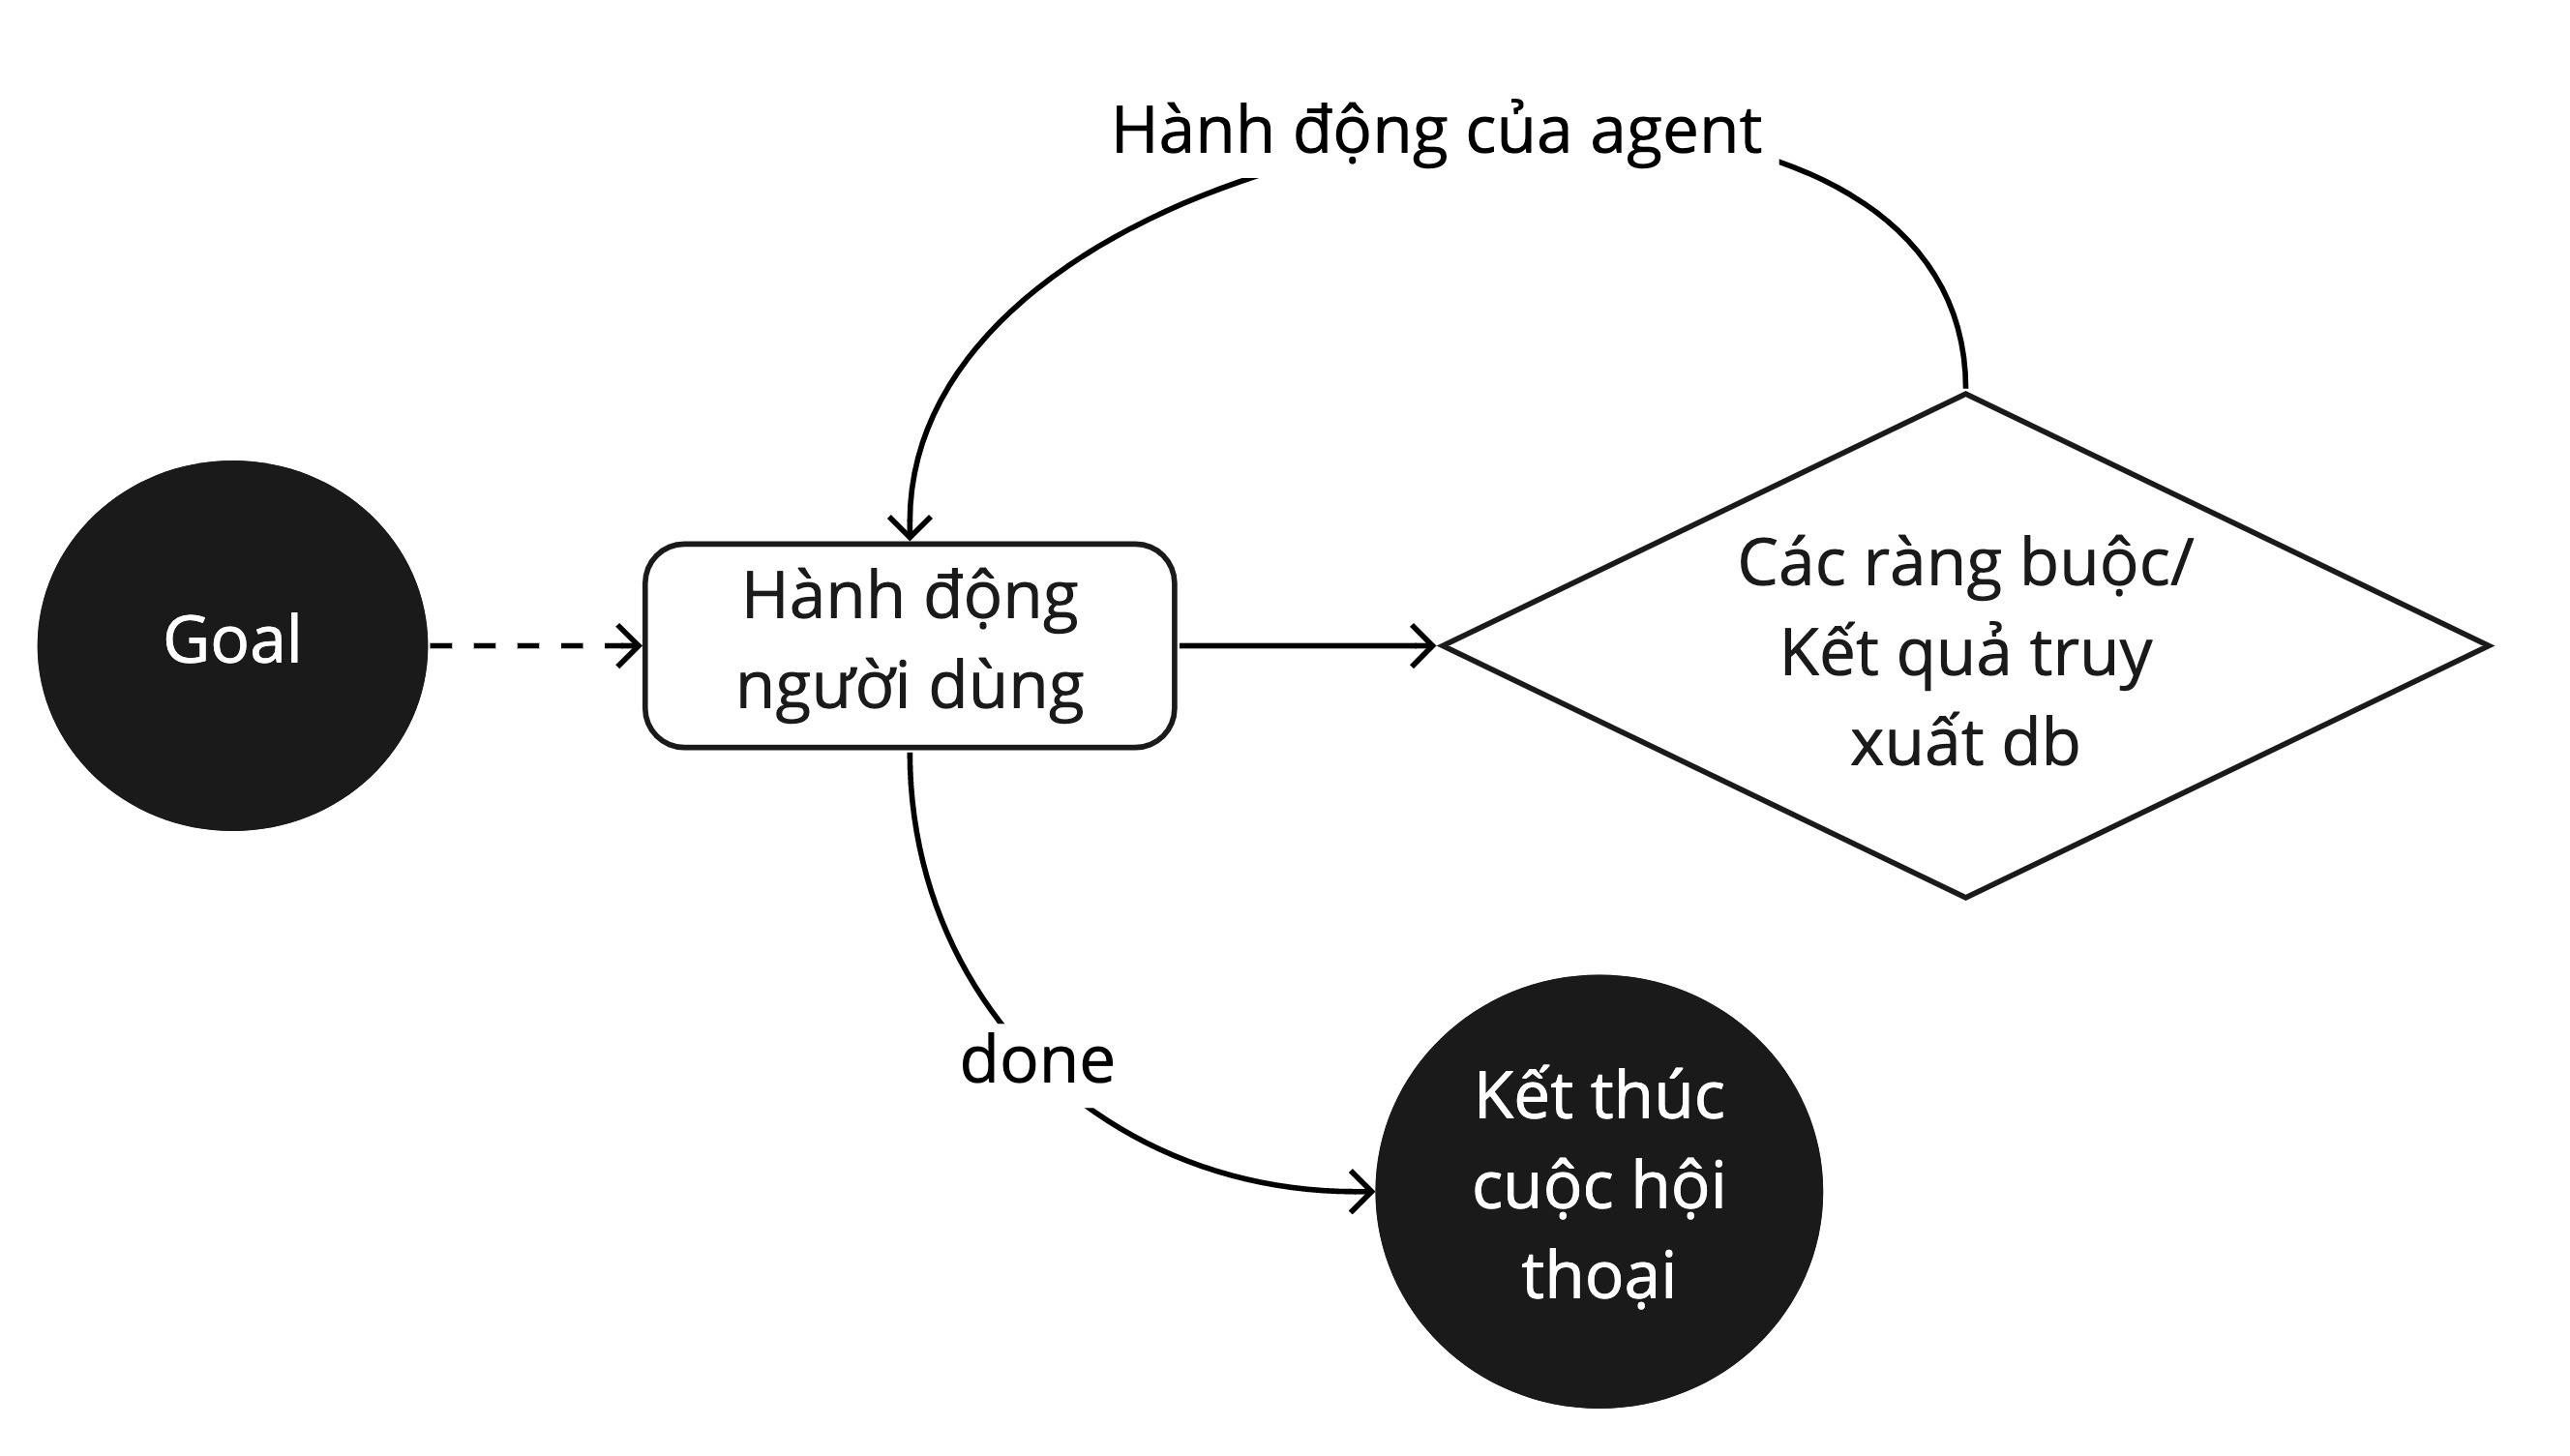
\includegraphics[scale=0.16]{thesis/chatbot/phuongphap/img/dialog.jpg}
    \caption{Sơ đồ biểu diễn tổng quát luật của hội thoại}
    \label{fig:dialog}
\end{figure}

Đầu tiên, ta xác định mục tiêu của người dùng trong hội thoại. Với
mục tiêu đó, lần lượt đưa ra các hành động tương ứng của người dùng,
qua mỗi lần nhận được hành động hệ thống sẽ kiểm tra các ràng buộc,
và trả về kết quả sau khi truy vấn lên cơ sở dữ liệu, tương ứng
đưa ra hành động cho tác nhân. Quá trình lặp lại cho đến khi
hoàn thành mục tiêu thì kết thúc hội thoại. Ví dụ một luật của
hội thoại cho mục tiêu yêu cầu giá bán sản phẩm có cấu trúc
như \ref{exam:rule}.

\renewcommand{\textboxenvname}{Ví dụ}
\begin{textbox}[exam:rule]{Luật của hội thoại cho mục tiêu yêu cầu giá bán sản phẩm}
\begin{Verbatim}[breaklines=true, breakanywhere=true]
"request_cost_product": [
    {
        "node": [
            {"id": 1, "intent": "request", "inform_slots": [], "request_slots": ["cost_product"]},
            {"id": 1, "intent": "request", "inform_slots": ["name_product"], "request_slots": ["cost_product"]},
            ...
        ],
        "condition": [
            {"id": 2, "rule": "exist", "entity": ["name_product"], "output": {"yes": 4, "no": 3}},
            ...
        ],
        "net": [
            {"Source": "start", "Destination": 1, "intent": "", "inform_slots": [], "request_slots": []},
            {"Source": 1, "Destination": 2, "intent": "check_condition", "inform_slots": [], "request_slots": []},
            ...
        ]
    }
]
\end{Verbatim}
\end{textbox}

\textit{Node} chứa các hành động của người dùng, gồm có \textit{id}
là số định danh hành động, \textit{intent} là ý định hành động
người dùng, và các danh sách chứa các thông tin yêu cầu hoặc
thông báo của người dùng. \textit{Condition} chứa các điều kiện
kiểm tra trạng thái hiện tại của hệ thống, và kết quả nhằm
điều hướng hành động kế tiếp. \textit{Net} chứa các hành động
của tác nhân hoặc tiến trình tiếp theo của hệ thống, gồm
\textit{source} chỉ điểm bắt đầu, \textit{destination} chỉ điểm đến,
\textit{intent} là ý định hành động của tác nhân hoặc chỉ hành vi
của hệ thống. Dựa trên bộ luật này, ta tạo ra các cuộc hội thoại có
cấu trúc như \ref{exam:dialog}, lần lượt là các hành động của
người dùng và tác nhân.

\renewcommand{\textboxenvname}{Ví dụ}
\begin{textbox}[exam:dialog]{Cuộc hội thoại được tạo bởi bộ luật}
\begin{Verbatim}[breaklines=true, breakanywhere=true]
[
    {"inform_slots": {}, "request_slots": {"cost_product": "UNK"}, "intent": "request", "speaker": "user"},
    {"intent": "request", "inform_slots": {}, "request_slots": {"name_product": "UNK"}, "speaker": "agent"},
    {"inform_slots": { "name_product": "dam hoa"}, "request_slots": {}, "intent": "inform", "speaker": "user"},
    {"intent": "inform", "inform_slots": {"cost_product": "160k"}, "request_slots": [], "speaker": "agent"},
    {"inform_slots": {}, "request_slots": {}, "intent": "ok", "speaker": "user"},
    {"intent": "match_found", "inform_slots": {}, "request_slots": {}, "speaker": "agent"},
    {"inform_slots": {}, "request_slots": {}, "intent": "ok", "speaker": "user"},
    {"intent": "done", "inform_slots": {}, "request_slots": {},"speaker": "agent"},
    {"inform_slots": {}, "request_slots": {}, "intent": "done", "speaker": "user"}
]
\end{Verbatim}
\end{textbox}

\subsubsection{Quá trình warmup}
Quá trình huấn luyện tác nhân trong giai đoạn warm-up được mô tả như
trong hình \ref{fig:warmupflow}.

\begin{figure}[ht!]
    \centering
    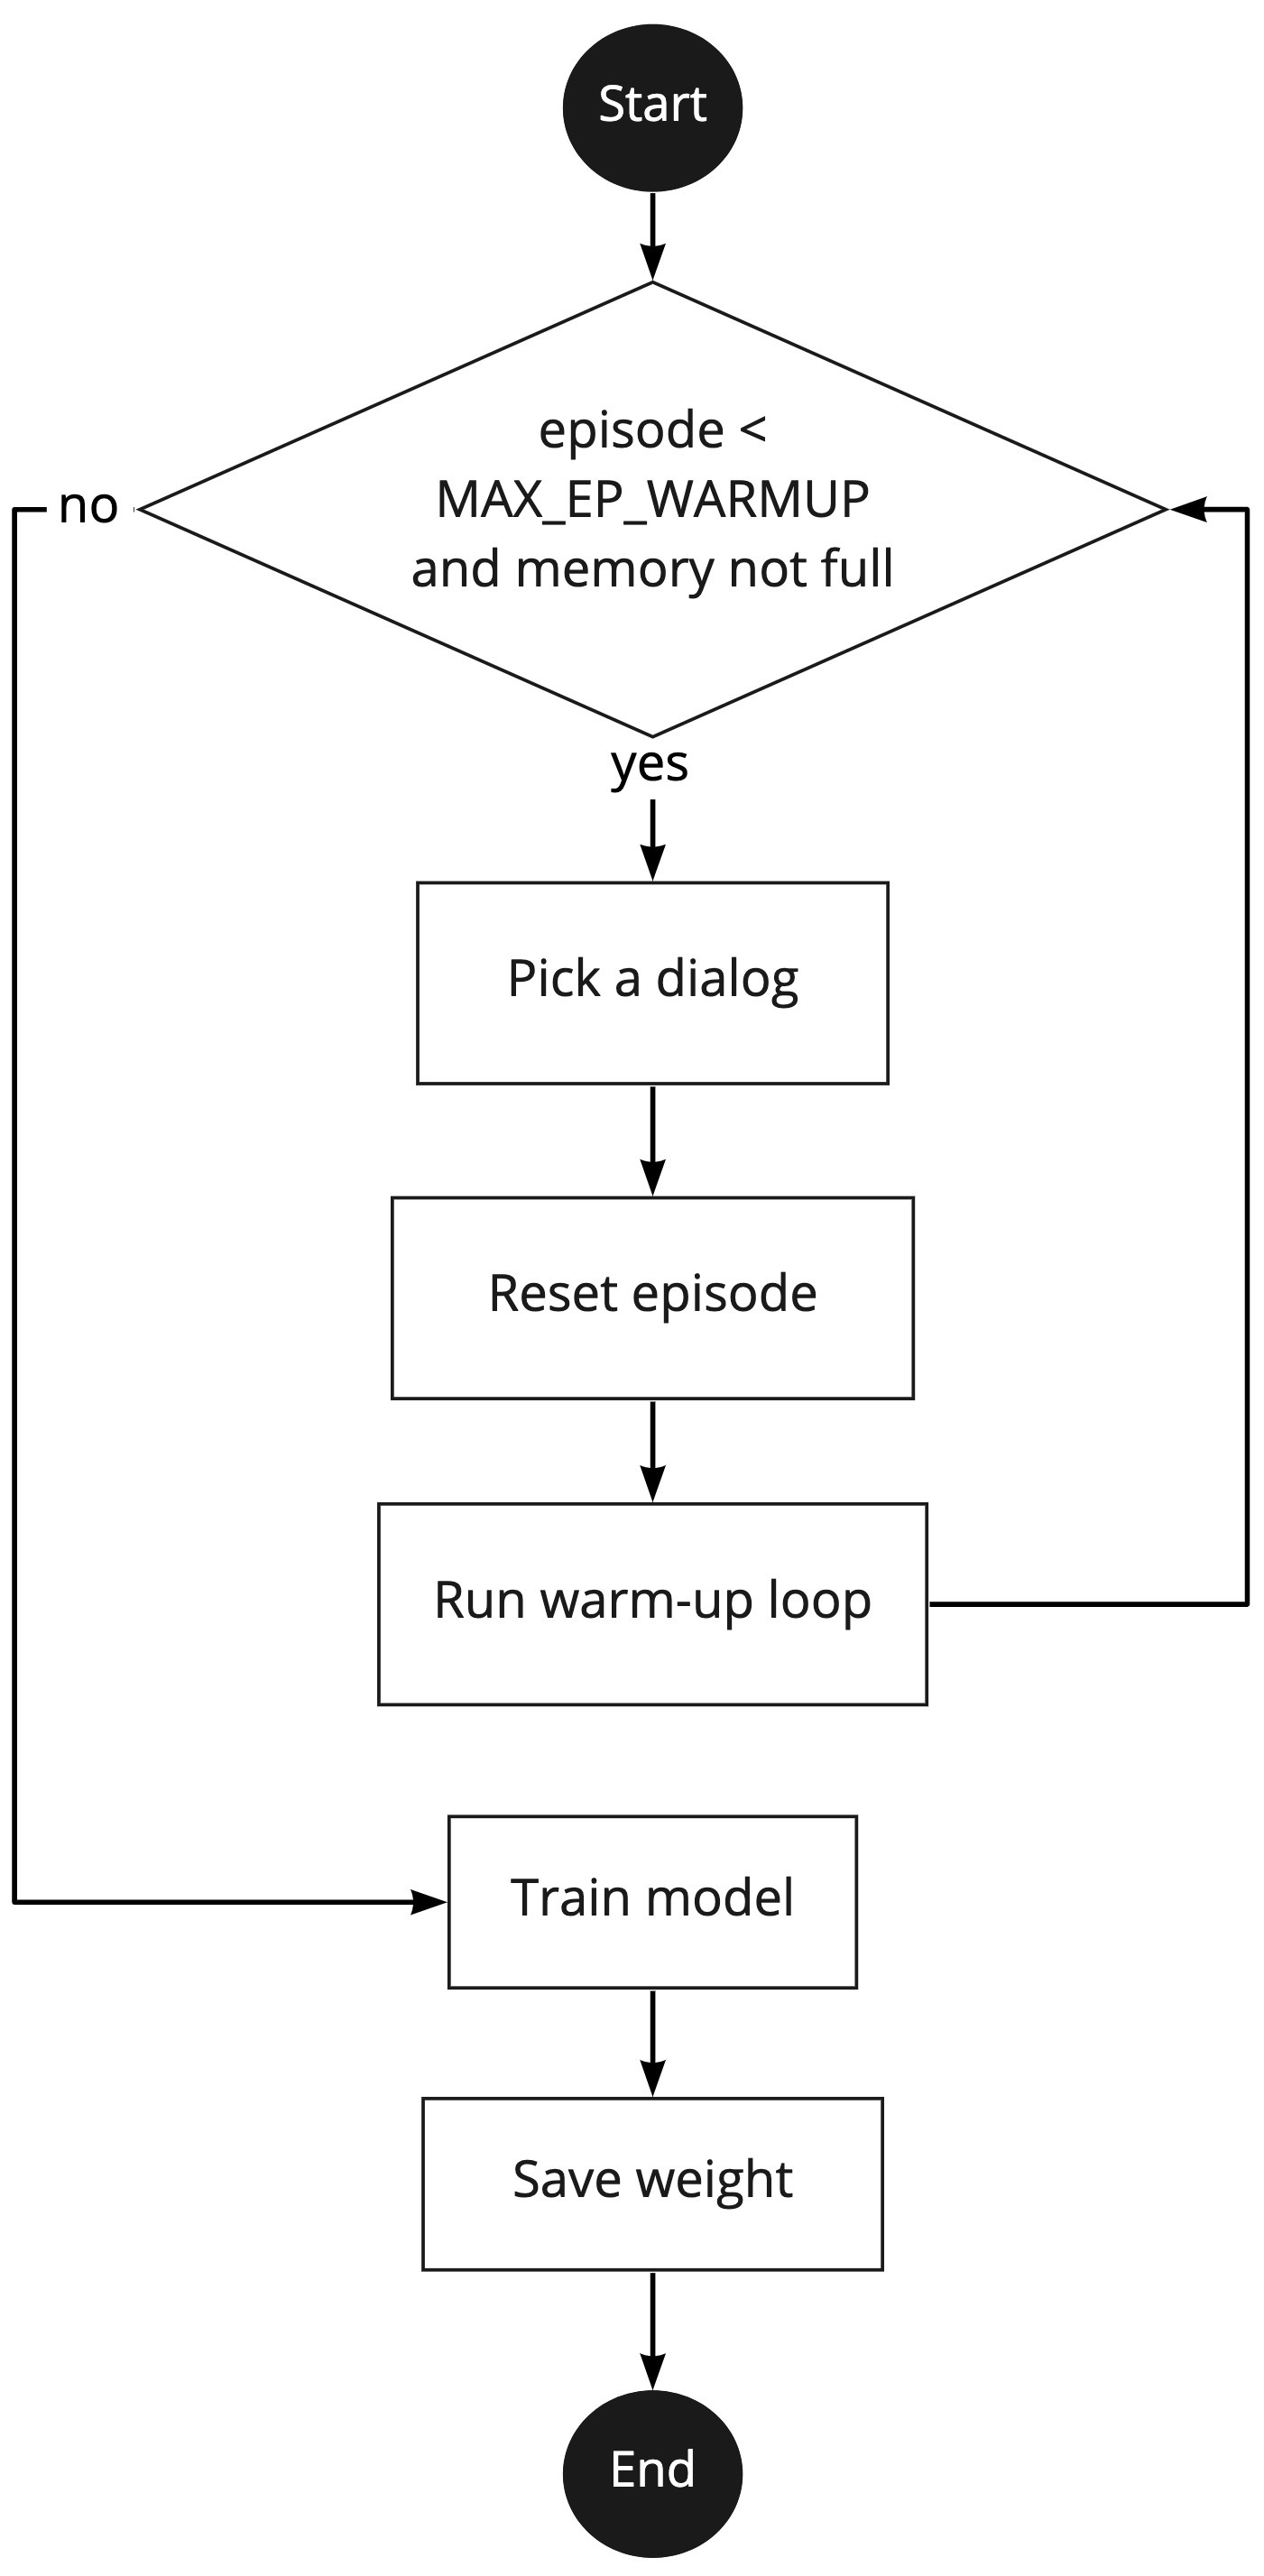
\includegraphics[scale=0.17]{thesis/chatbot/phuongphap/img/warmup_flow.jpg}
    \caption{Sơ đồ quá trình huấn luyện mô hình - giai đoạn warm-up}
    \label{fig:warmupflow}
\end{figure}

Đầu tiên, ta kiểm tra số lượt hội thoại hiện tại đã được thực hiện
không vượt quá số lượt lớn nhất chỉ định và bộ nhớ của tác nhân
còn trống. Kế tiếp, ta lấy một hội thoại (dialog) trong dữ liệu
các bộ hội thoại đã được tạo trước đó. Hội thoại này sẽ được
sử dụng cho các quyết định hành động sau này. Khởi tạo và thiết lập
lại toàn bộ thông tin của cuộc hội thoại như trạng thái, hành động
của người dùng, tác nhân, ... Trong đó, ta có khởi tạo hành động
đầu tiên của người dùng, ở đây là lấy hành động đầu tiên trong
hội thoại và gửi nó đến bộ quản lý trạng thái hội thoại. Sau đó
thực hiện vòng lặp warm-up được mô tả cụ thể ở hình
\ref{fig:warmup}. Sau khi hoàn tất quá trình khởi tạo ký ức cho
tác nhân, ta sẽ mang toàn bộ ký ức này đem đi huấn luyện cho
mô hình mạng nơ-ron sẽ được trình bày ở phần \ref{subsec:agent}.

Hình \ref{fig:warmup} mô tả một vòng lặp warm-up.

\begin{figure}[ht!]
    \centering
    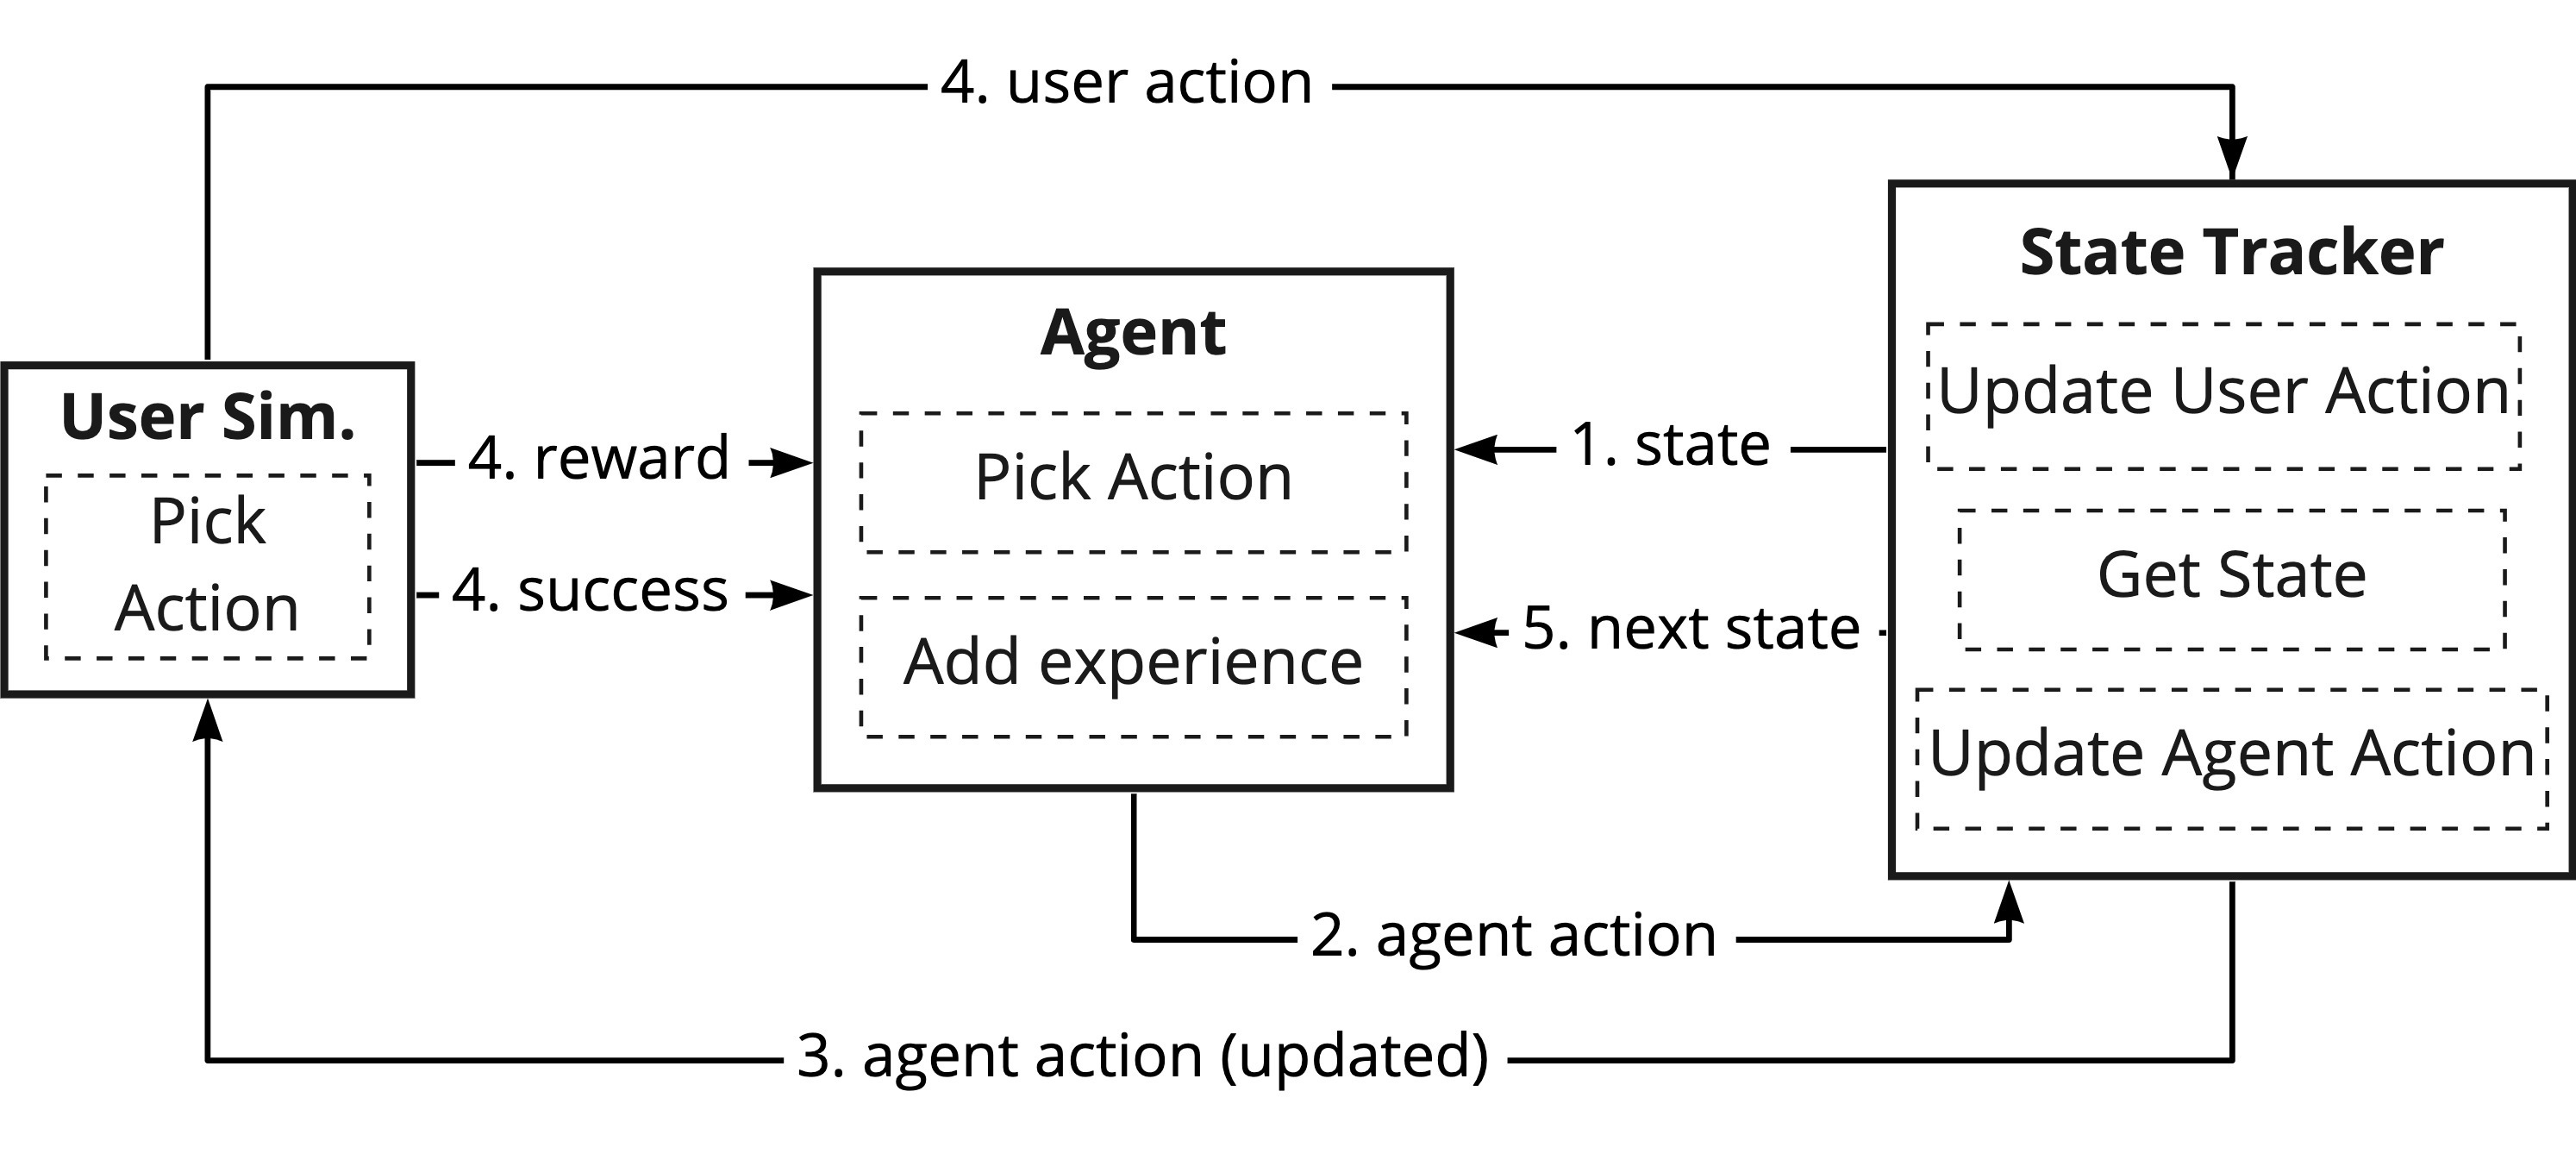
\includegraphics[scale=0.14]{thesis/chatbot/phuongphap/img/warmup.jpg}
    \caption{Vòng lặp huấn luyện - giai đoạn warm-up}
    \label{fig:warmup}
\end{figure}

Mỗi một vòng thực hiện là một lượt đối thoại qua lại giữa người dùng
và tác nhân. Cụ thể:

\begin{itemize}
    \item \textbf{Bước 1:} Ta lấy ra \textit{state} - trạng thái
    hiện tại của hội thoại từ \textit{State Tracker} - bộ quản lý
    trạng thái hội thoại, trạng thái này có thể là trạng thái
    khởi tạo nếu như vừa bắt đầu hội thoại hoặc là trạng thái của
    toàn bộ cuộc hội thoại giữa người dùng và tác nhân. Mục đích lấy
    trạng thái ở giai đoạn này là để ghi vào bộ nhớ, và sẽ làm
    dữ liệu đầu vào (input) cho việc huấn luyện mô hình sau này.
    \item \textbf{Bước 2:} Tác nhân sau khi nhận được input từ
    bước trước sẽ lưu vào kí ức (experience) của nó và lấy ra một
    \textit{action} (hành động) từ trong \textit{dialog} và gửi
    ngược về lại bộ quản lý trạng thái hội thoại. Ở đây, nó sẽ được
    bộ quản lý trạng thái hội thoại cập nhật số lượt đã được
    thực hiện trong hội thoại. Đồng thời bộ quản lý trạng thái
    hội thoại cũng sẽ cập nhật lại trạng thái của hội thoại.
    \item \textbf{Bước 3:} Hành động sau khi được cập nhật đầy đủ
    thông tin sẽ được gửi cho \textit{User Simulator} - bộ
    mô phỏng người dùng. Bộ mô phỏng người dùng cũng dựa vào
    \textit{dialog}, lấy ra một hành động, đồng thời sẽ dựa vào
    các luật đã được quy định trước để chấm \textit{reward}
    (điểm thưởng) và tín hiệu success (thành công) để giúp tác nhân
    có thể tự điều chỉnh hành vi để học. Ở đây, tác nhân cũng sẽ
    ghi lại toàn bộ vào ký ức của nó.
    \item \textbf{Bước 4:} Hành động của người dùng ở bước trước sẽ
    tiếp tục được gửi đi đến bộ quản lý trạng thái hội thoại và
    được cập nhật thông tin cụ thể tương tự ở bước 2. Đồng thời
    bộ quản lý trạng thái hội thoại cũng cập nhật trạng thái của nó.
    \item \textbf{Bước 5:} Trạng thái tiếp theo được lấy từ bộ
    quản lý trạng thái hội thoại và quay lại giống bước 1.
\end{itemize}

Quá trình này sẽ được thực hiện liên tục cho đến khi thực thi
lần lượt hết tất cả các hành động của người dùng và
tác nhân trong \textit{dialog}.

\subsubsection{Ví dụ}
Như trình bày ở trên, trong giai đoạn warm-up, ta sẽ lấy một đoạn
hội thoại được tạo sẵn. Xét mẫu hội thoại như ví dụ
\ref{exam:dialog3}. Giả sử, trạng thái chỉ chứa các ý định hành động
hiện tại của người dùng lần lượt là: hello, inform, request, reject,
done. Ta mã hóa về dạng one-hot vec-tơ để làm đầu vào cho mạng
nơ-ron. Quá trình huấn luyện trong giai đoạn warm-up như sau:

\begin{itemize}
    \item Đầu tiên, bộ mô phỏng người dùng sẽ lấy hành động đầu tiên
    trong hội thoại là yêu cầu thông tin màu sắc (request(cost\_product)).
    Sau đó nó được gửi tới bộ quản lý trạng thái hội thoại. Bộ quản lý
    trạng thái hội thoại sẽ thêm thông tin số lượt thực hiện là 1 vào
    hành động của người dùng để kiểm soát hội thoại kéo dài không quá
    số lượt cho phép (20). Đồng thời lấy trạng thái hiện tại của hội thoại
    gửi qua cho tác nhân là $[0\; 0\; 1\; 0\; 0]$. Quá trình được
    biểu diễn như hình \ref{fig:examwarmup}.
\end{itemize}

\begin{figure}[ht!]
    \centering
    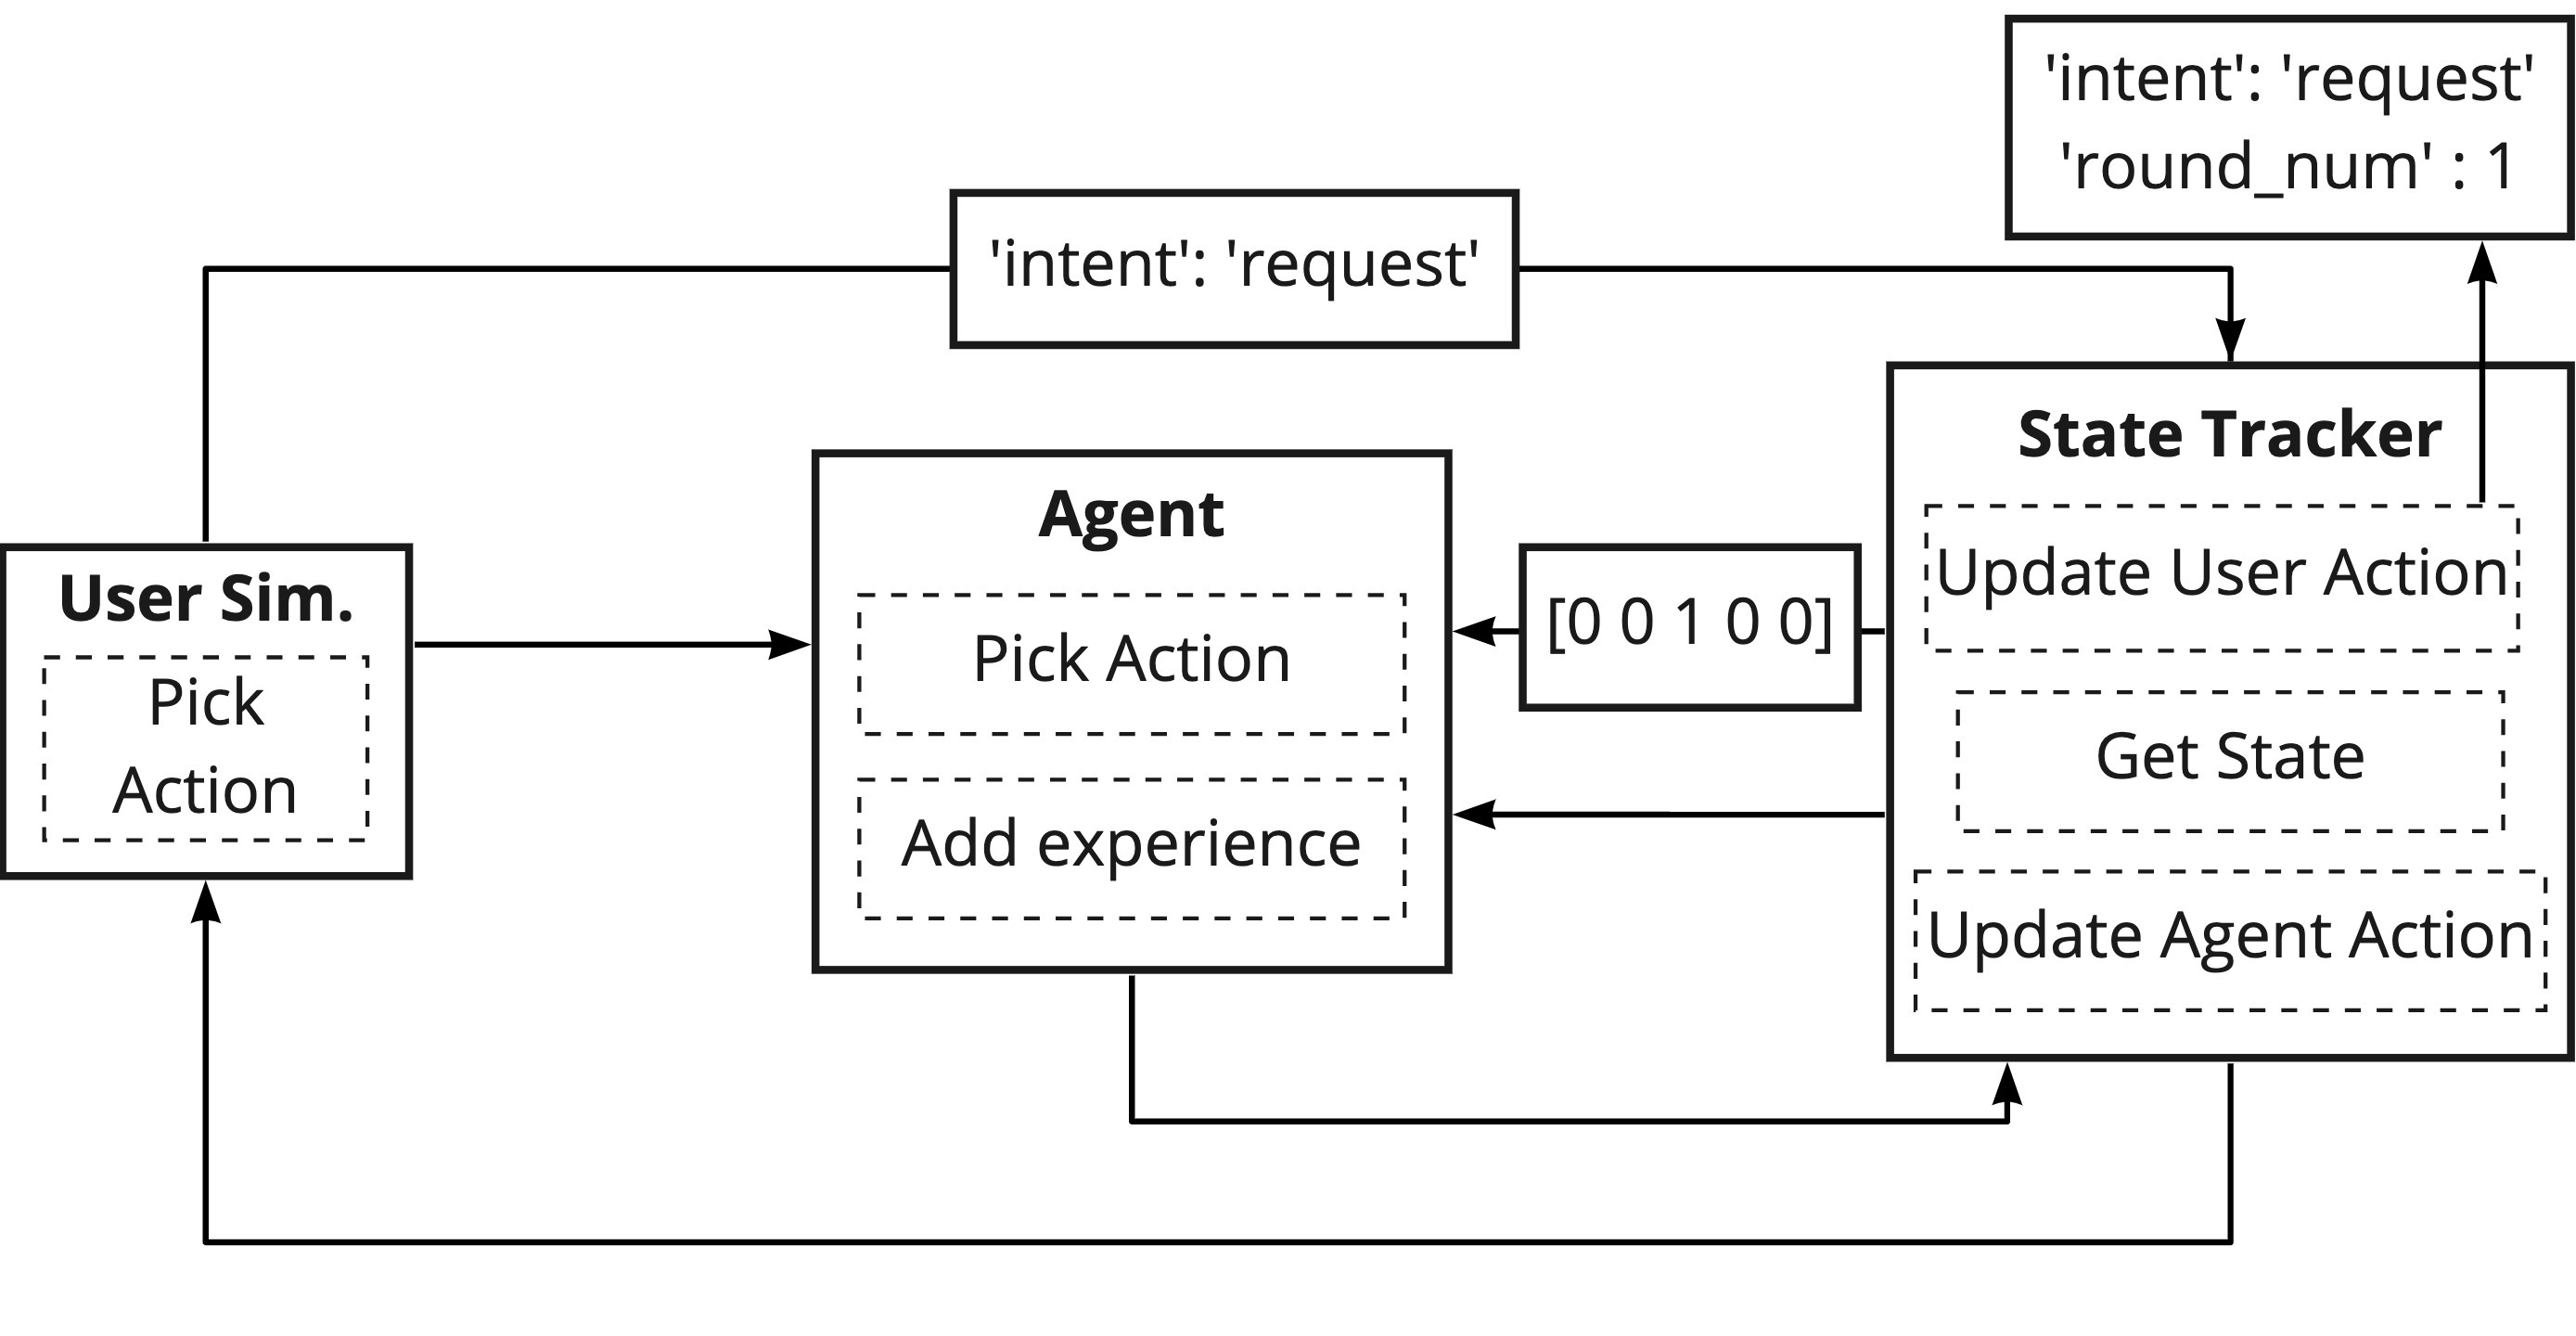
\includegraphics[scale=0.15]{thesis/chatbot/phuongphap/img/warmup_exam.jpg}
    \caption{Ví dụ quá trình huấn luyện bước 1 - giai đoạn warm-up}
    \label{fig:examwarmup}
\end{figure}

\begin{itemize}
    \item Tại đây, tác nhân sẽ lấy hành động kế tiếp trong hội thoại
    là yêu cầu tên sản phẩm (request(name\_product)). Sau đó nó được
    gửi tới bộ quản lý trạng thái hội thoại. Tương tự, bộ quản lý
    trạng thái hội thoại sẽ thêm thông tin số lượt thực hiện vào
    hành động của tác nhân là 1 và gửi qua cho bộ mô phỏng người dùng.
    Quá trình được biểu diễn như hình \ref{fig:examwarmup1}.
\end{itemize}

\begin{figure}[ht!]
    \centering
    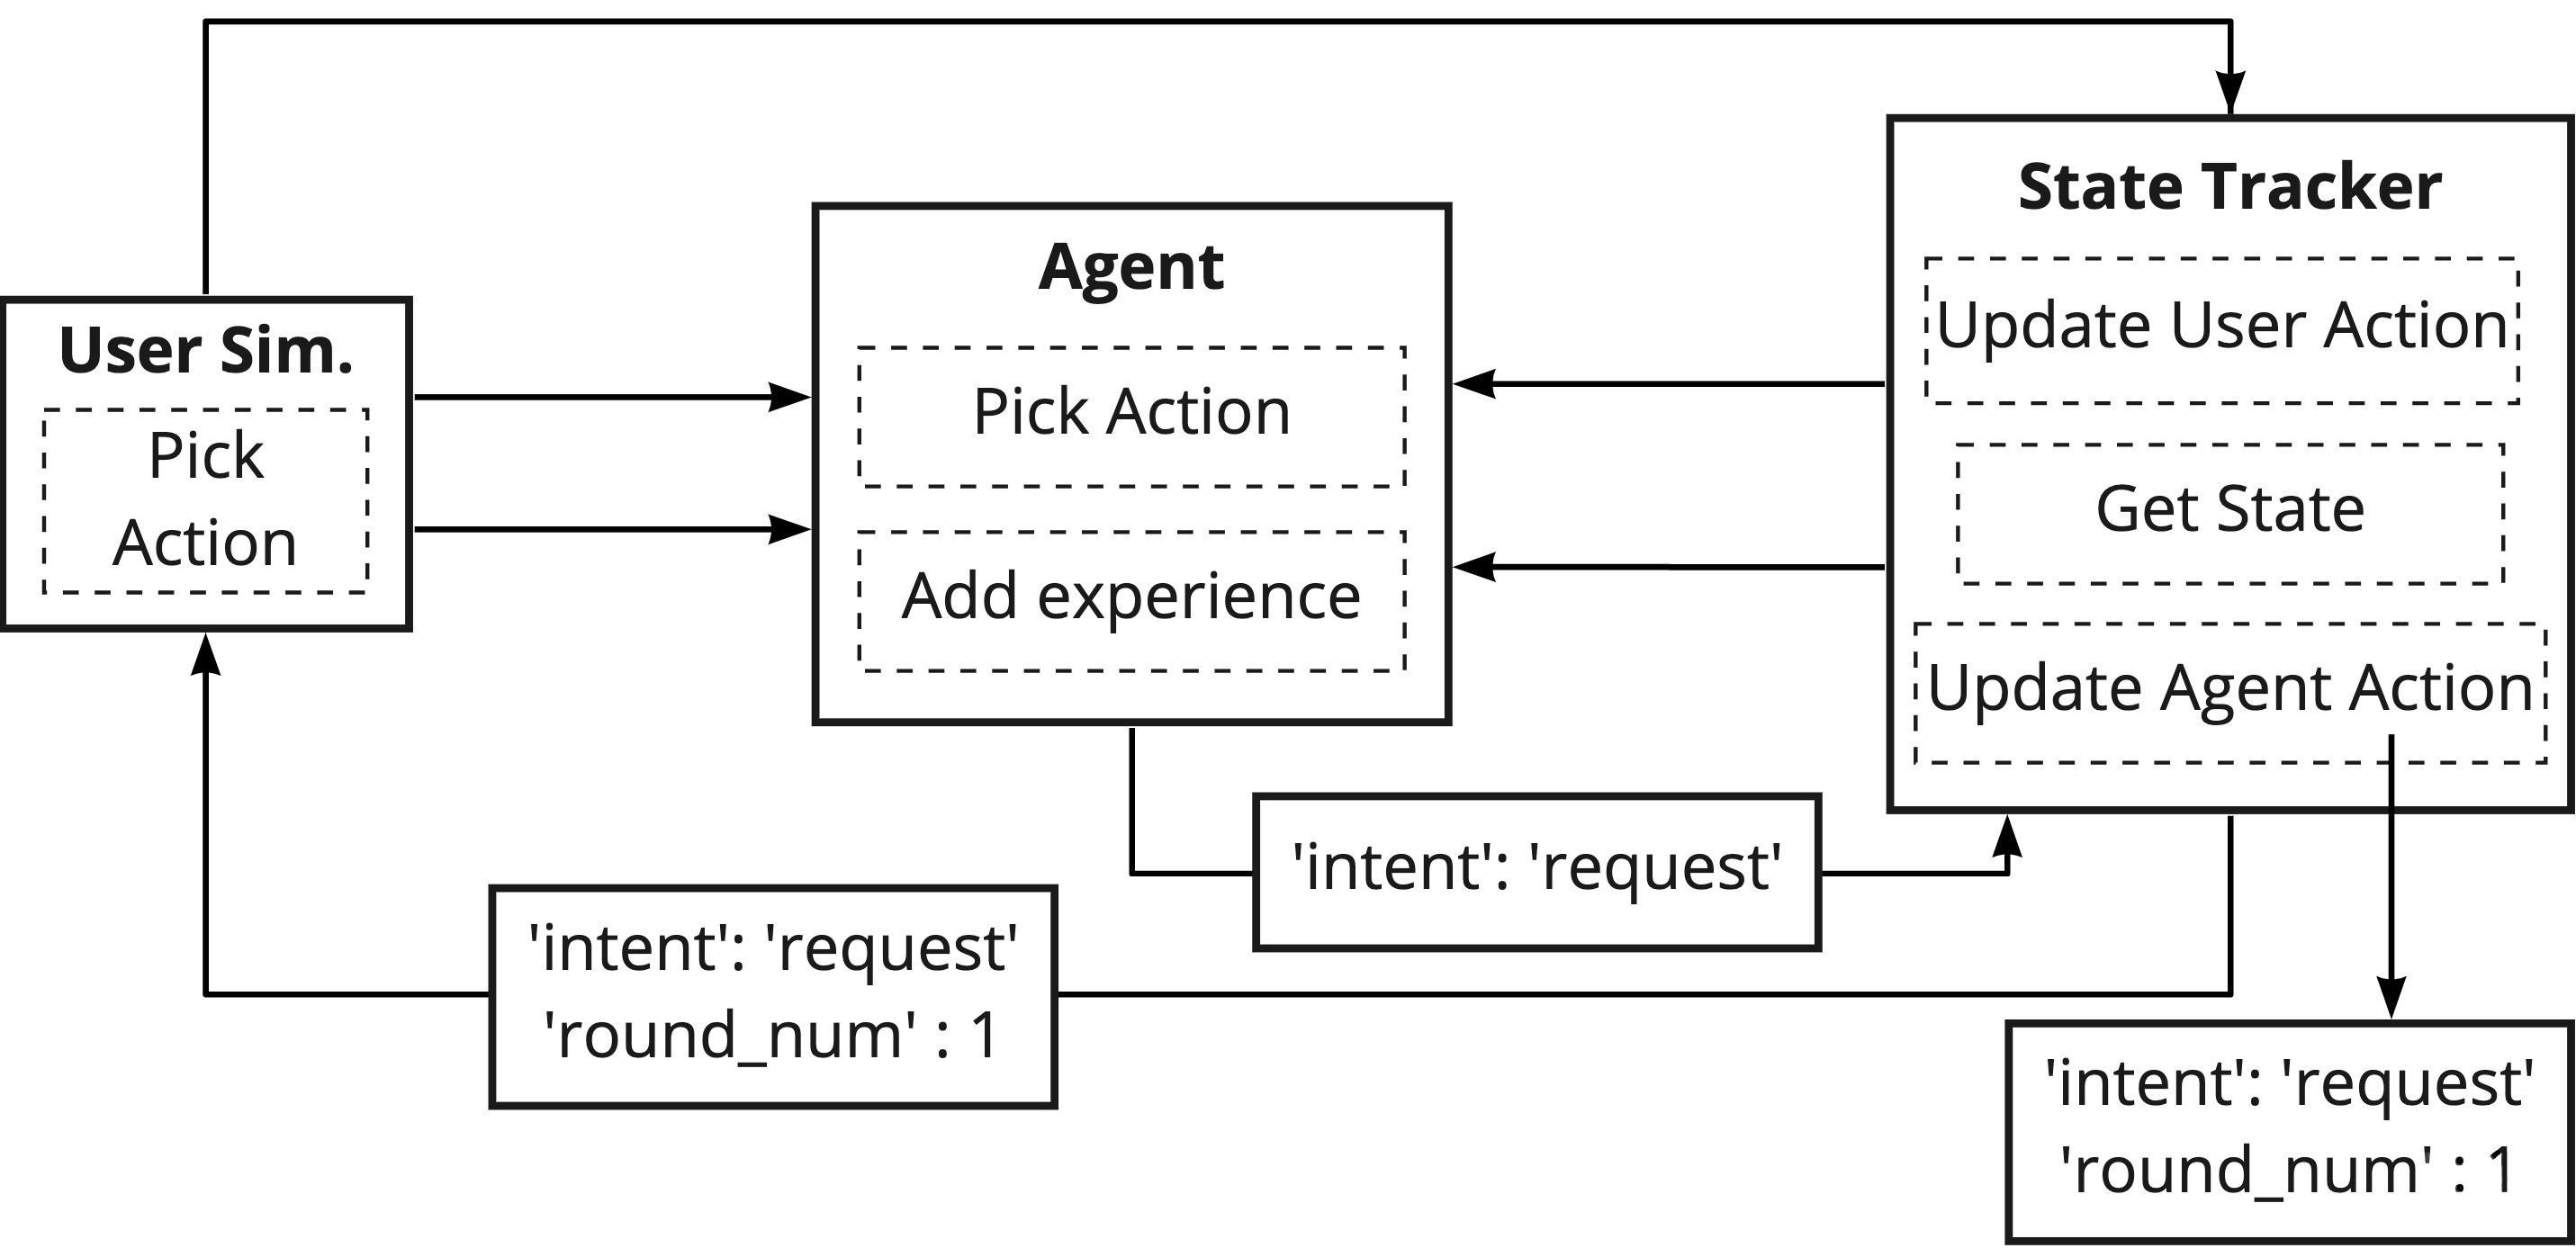
\includegraphics[scale=0.15]{thesis/chatbot/phuongphap/img/warmup_exam1.jpeg}
    \caption{Ví dụ quá trình huấn luyện bước 2 - giai đoạn warm-up}
    \label{fig:examwarmup1}
\end{figure}

\begin{itemize}
    \item Tương tự, bộ mô phỏng người dùng sẽ lấy hành động kế tiếp
    trong hội thoại là thông báo tên sản phẩm (inform(name\_product)).
    Gửi tới bộ quản lý trạng thái hội thoại. Bộ quản lý trạng thái
    hội thoại sẽ thêm thông tin số lượt vào hành động của người dùng
    là 2. Cập nhật và lấy trạng thái hiện tại của hội thoại gửi qua
    cho tác nhân là $[0\; 1\; 0\; 0\; 0]$. Ngoài ra, bộ mô phỏng
    người dùng cũng sẽ gửi điểm thưởng cho phản hồi vừa rồi của
    tác nhân (request(name\_product)). Với cách cho điểm thưởng như
    được mô tả ở mục \ref{subsec:reward}. Ta giả sử, điểm thưởng là
    -1. Quá trình được biểu diễn như hình \ref{fig:examwarmup2}.
\end{itemize}

\begin{figure}[ht!]
    \centering
    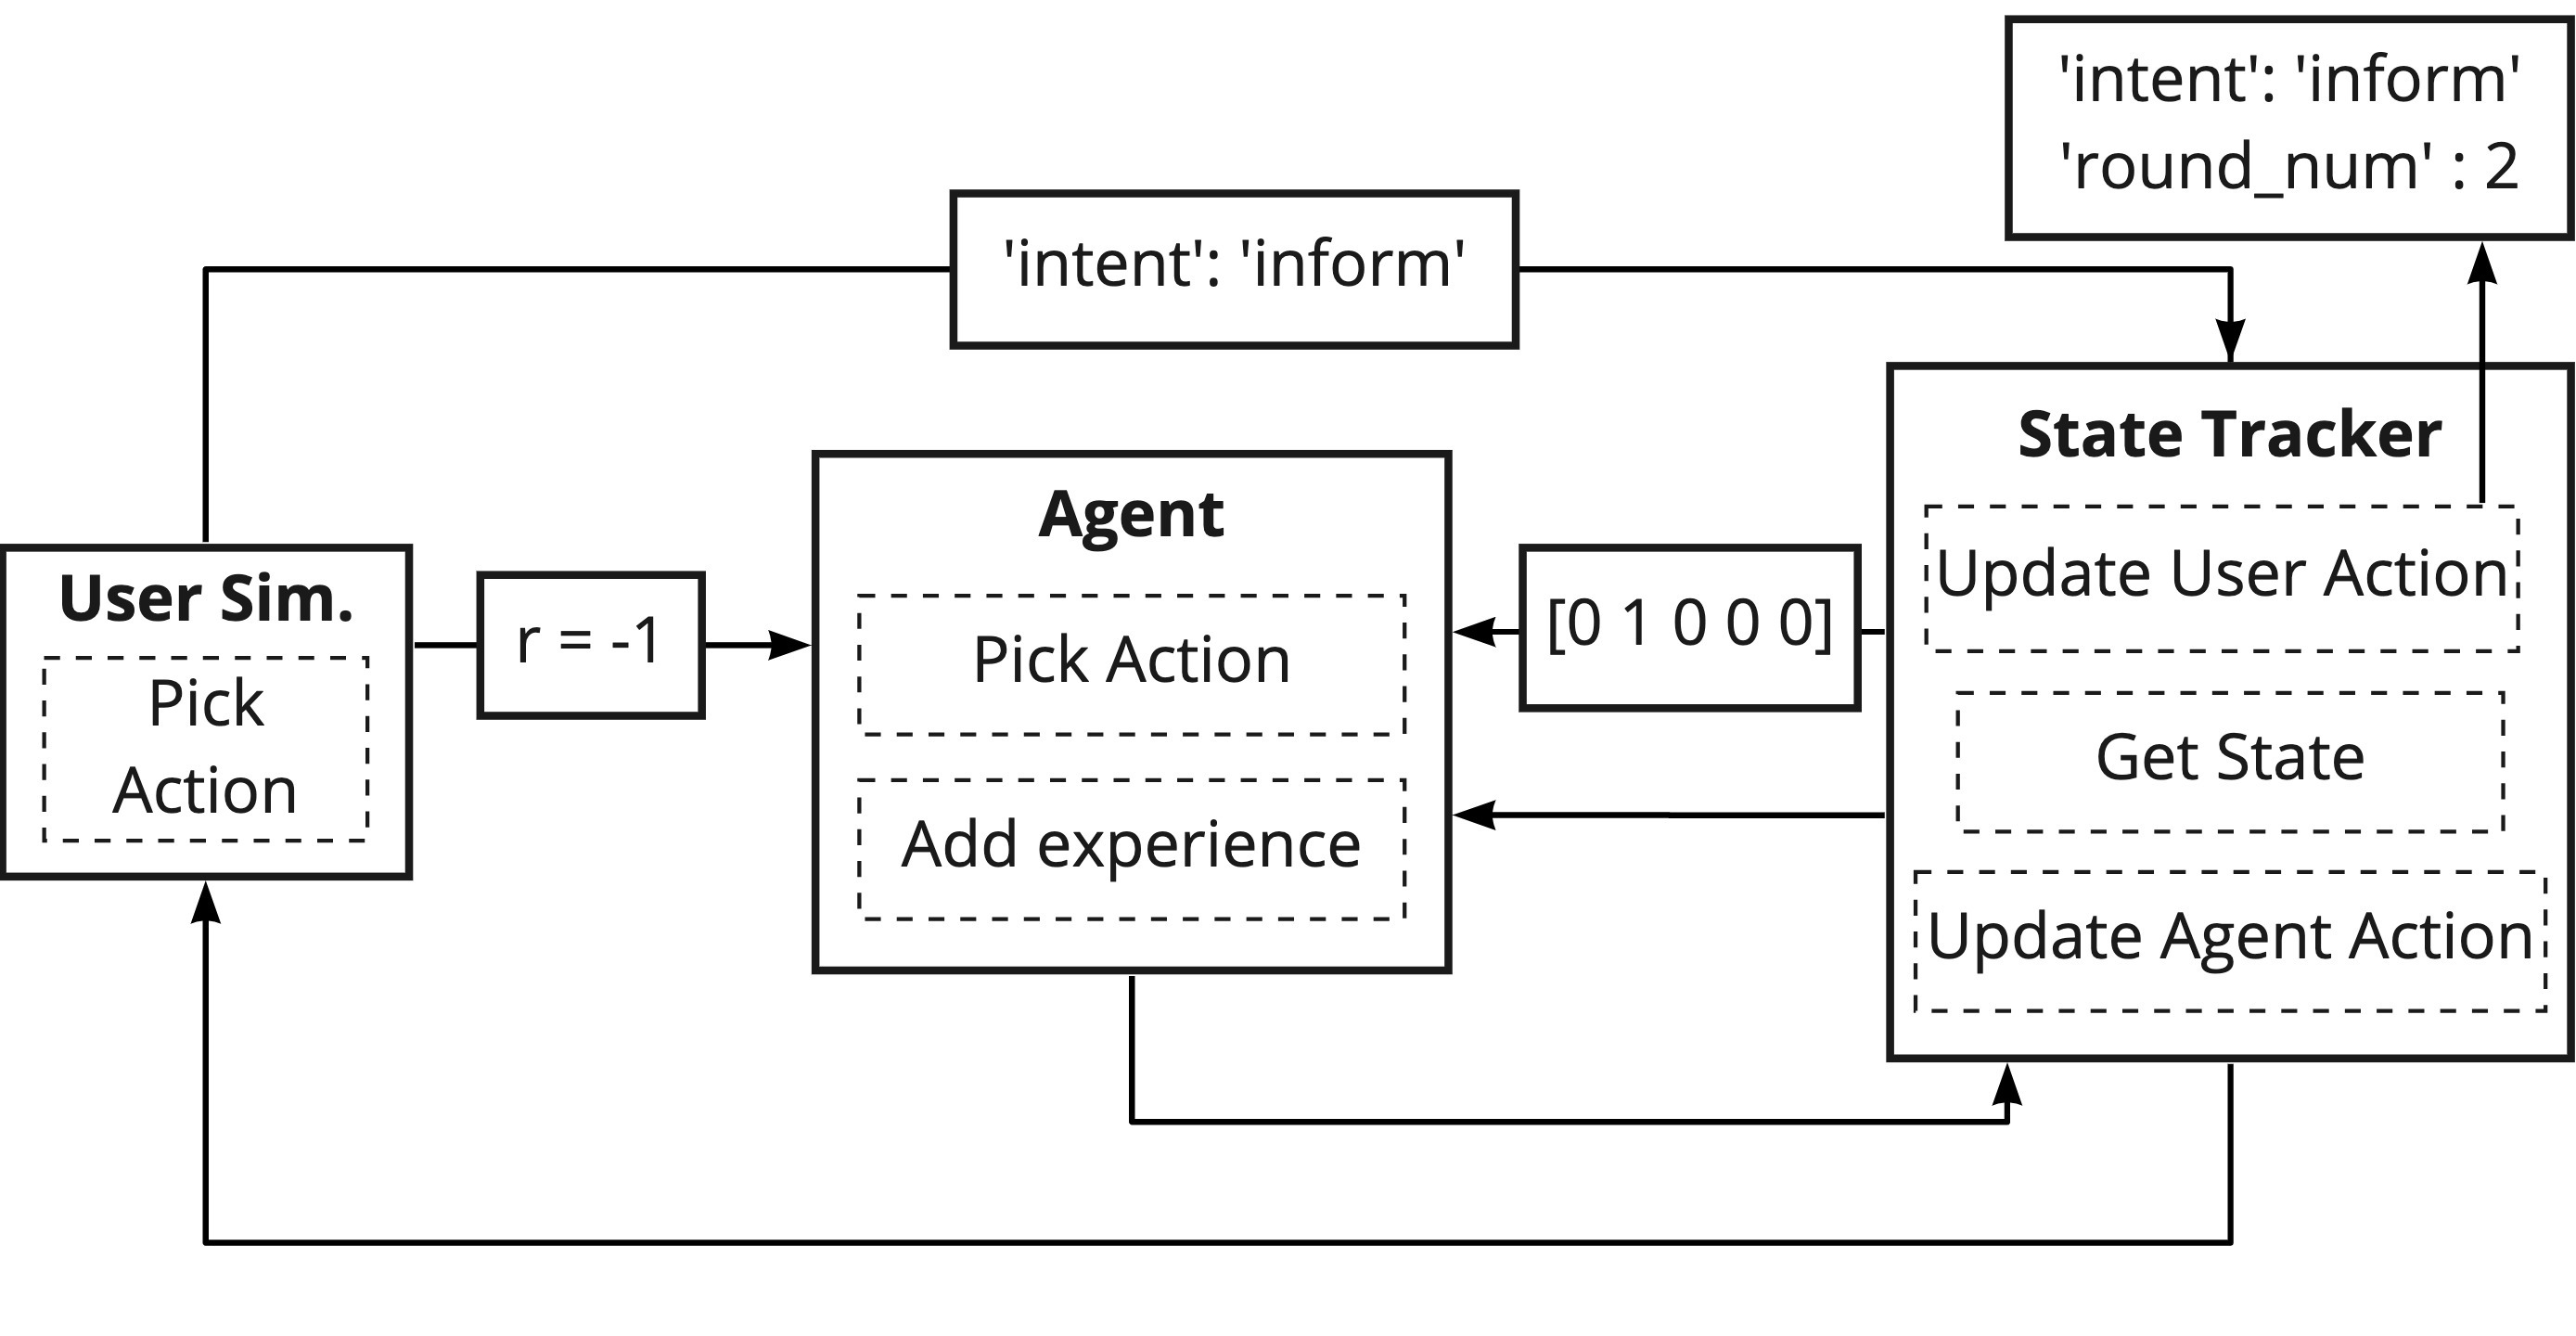
\includegraphics[scale=0.15]{thesis/chatbot/phuongphap/img/warmup_exam2.jpg}
    \caption{Ví dụ quá trình huấn luyện bước 3, 4 và 5 - giai đoạn warm-up}
    \label{fig:examwarmup2}
\end{figure}

Trạng thái hội thoại tại thời điểm này chính là trạng thái kế tiếp
của hành động trước đó (request(cost\_product)) của người dùng.

Tại đây, chúng ta đã có đầy đủ thông tin:
\begin{itemize}
    \item State ($s$): trạng thái hiện tại khi người dùng yêu cầu
    thông tin (request(cost\_product)) là $[0\; 0\; 1\; 0\; 0]$.
    \item Next state ($s'$): trạng thái kế tiếp của người dùng
    sau khi tác nhân phản hồi yêu cầu tên sản phẩm
    (request(name\_product)) là $[0\; 1\; 0\; 0\; 0]$.
    \item Action ($a$): hành động tác nhân phản hồi tại
    trạng thái $s$ là request(name\_product).
    \item Reward ($r_0$): phần thưởng cho hành động $a$ là -1
\end{itemize}

Toàn bộ thông tin này được lưu vào bộ nhớ. Sau khi quá trình
ghi nhớ các hội thoại mẫu này kết thúc. Ta sẽ thực hiện việc
huấn luyện như mô tả ở mục \ref{subsec:deepqlearning}

\subsection{Giai đoạn huấn luyện (Training stage)}

\subsubsection{Mục tiêu}
Đây là quá trình chính nhằm mục đích huấn luyện cho tác nhân có
khả năng thực hiện các hành động tương tự như con người, có
khả năng đáp trả giúp người dùng hoàn thành được mục tiêu khi
tham gia cuộc hội thoại. Quá trình huấn luyện sử dụng tập dữ liệu
\textit{User Goal}, chứa các mục tiêu của người dùng làm đầu vào
cho bộ mô phỏng người dùng. Dựa vào mục tiêu trên, bộ mô phỏng
người dùng tự đưa ra các hành động phù hợp. Tác nhân với kí ức trước
đã được học ở giai đoạn warm-up, đưa ra hành động phản hồi và
được huấn luyện lại sau một số lượt hội thoại diễn ra.

\subsubsection{Quá trình training}
Quá trình huấn luyện tác nhân trong giai đoạn training được mô tả
như trong hình \ref{fig:trainingflow}

\begin{figure}[!ht]
    \centering
    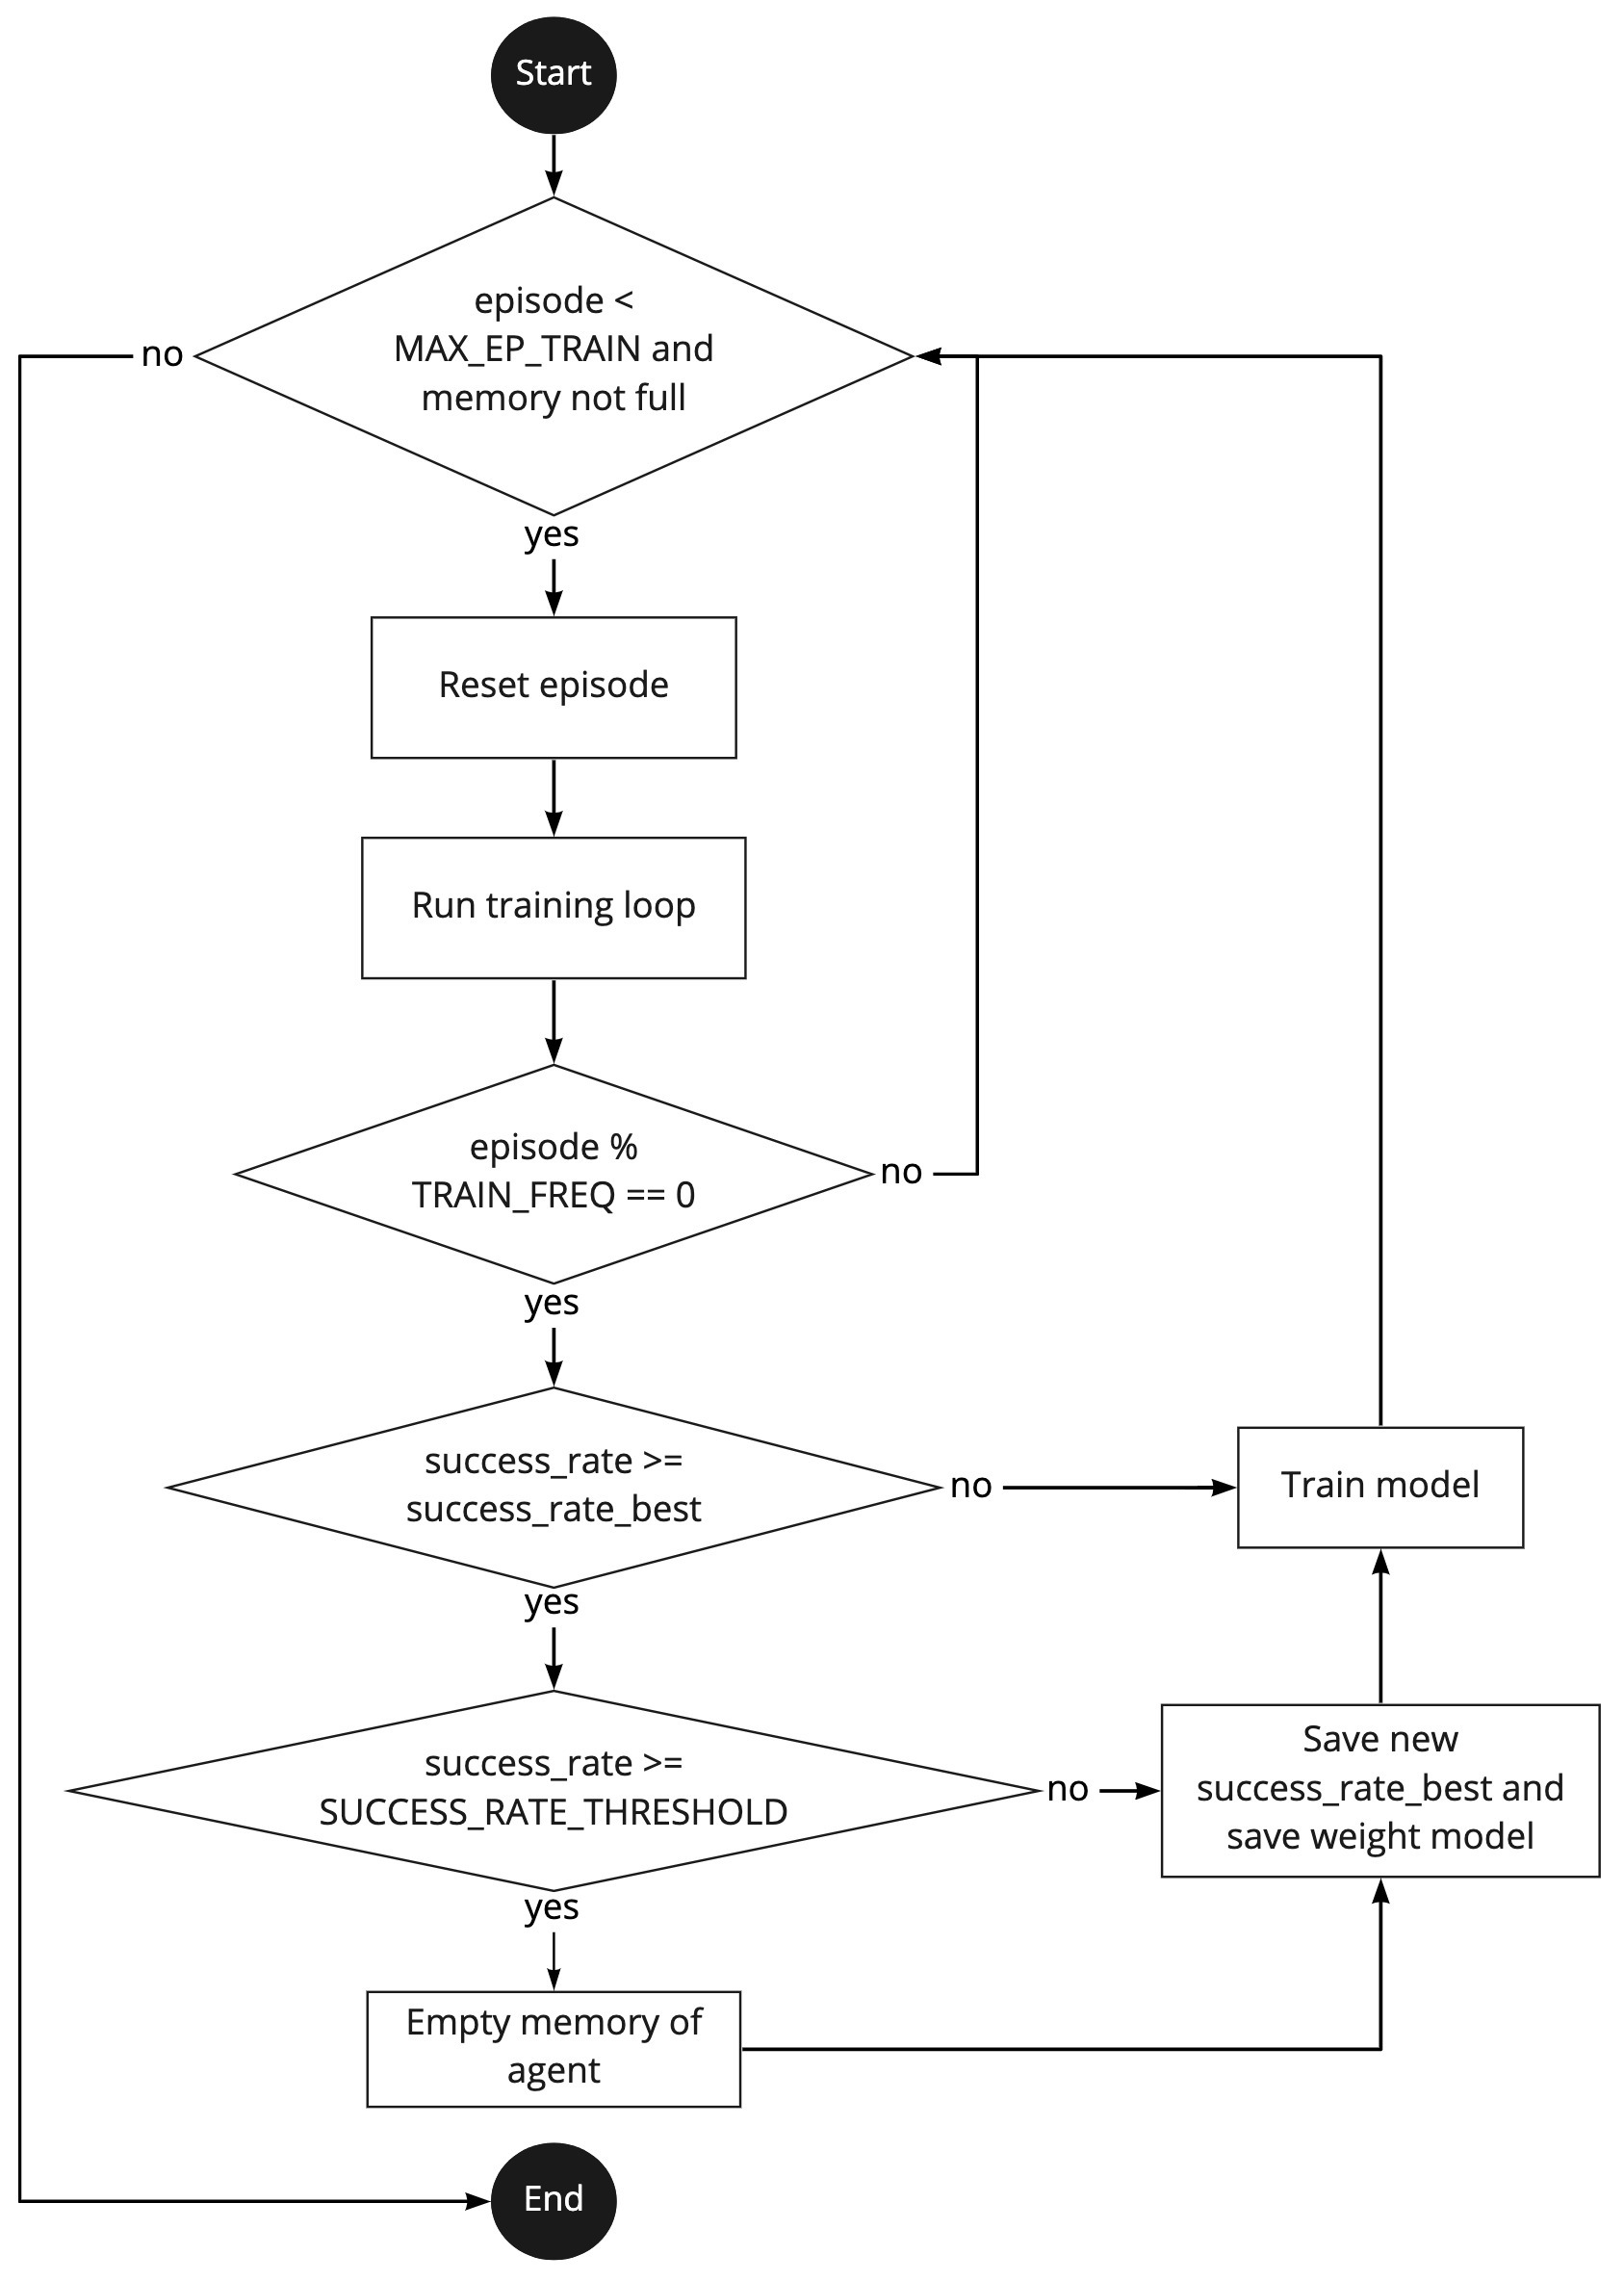
\includegraphics[scale=0.24]{thesis/chatbot/phuongphap/img/training_flow.jpg}
    \caption{Sơ đồ quá trình huấn luyện mô hình - giai đoạn training}
    \label{fig:trainingflow}
\end{figure}

Đầu tiên, giống với giai đoạn warm-up, ta kiểm tra số lượt hội thoại
hiện tại đã được thực hiện không vượt quá số lượt lớn nhất chỉ định
và bộ nhớ của tác nhân còn trống. Kế tiếp, quá trình khởi tạo và
thiết lập lại toàn bộ thông tin của cuộc hội thoại được thực hiện như
xóa lịch sử trạng thái, hành động của người dùng, tác nhân, ...
Tại bước này, bộ mô phỏng người dùng đồng thời lấy một mục tiêu
người dùng trong cơ sở dữ liệu, tạo ra hành động đầu tiên trong
cuộc hội thoại và lấy nó làm mục tiêu trong suốt cuộc hội thoại
diễn ra. Sau đó, là quá trình thực hiện vòng lặp training cho đến khi
kết thúc cuộc hội thoại. Vòng lặp này sẽ được mô tả cụ thể ở hình
\ref{fig:training}. Vòng lặp sẽ kết thúc sau mỗi lần cuộc hội thoại
được hoàn thành (thành công hoặc thất bại). Cứ mỗi một số hội thoại
nhất định được hoàn thành (được xác định bởi tham số
\textit{TRAIN\_FREQ}), ta kiểm tra tỉ lệ thành công trong số các
cuộc hội thoại đó. Nếu hiện tại là lớn nhất và lớn hơn một mức ngưỡng
cho trước thì xóa đi toàn bộ ký ức của tác nhân. Việc này nhằm
mục đích để tác nhân loại bỏ đi các trải nghiệm cũ, khi mà những
trải nghiệm đó đưa ra những quyết định không tốt, thì tốt hơn hết
chúng ta sẽ huấn luyện nó với phiên bản tốt hơn. Nếu không ta vẫn
giữ lại các ký ức đó và lưu lại tỉ lệ thành công tốt nhất và trọng số
của mô hình. Ở đây, ta có một tác nhân được huấn luyện với trạng thái
tốt nhất hiện tại. Nếu tỉ lệ thành công hiện tại không lớn nhất,
thì ta chỉ tiếp tục huấn luyện mô hình với những ký ức đang có.
Quá trình huấn luyện này sẽ kết thúc cho đến khi hết số lượt hội thoại
cần huấn luyện.

Hình \ref{fig:training} mô tả một vòng lặp training.

\begin{figure}[ht!]
    \centering
    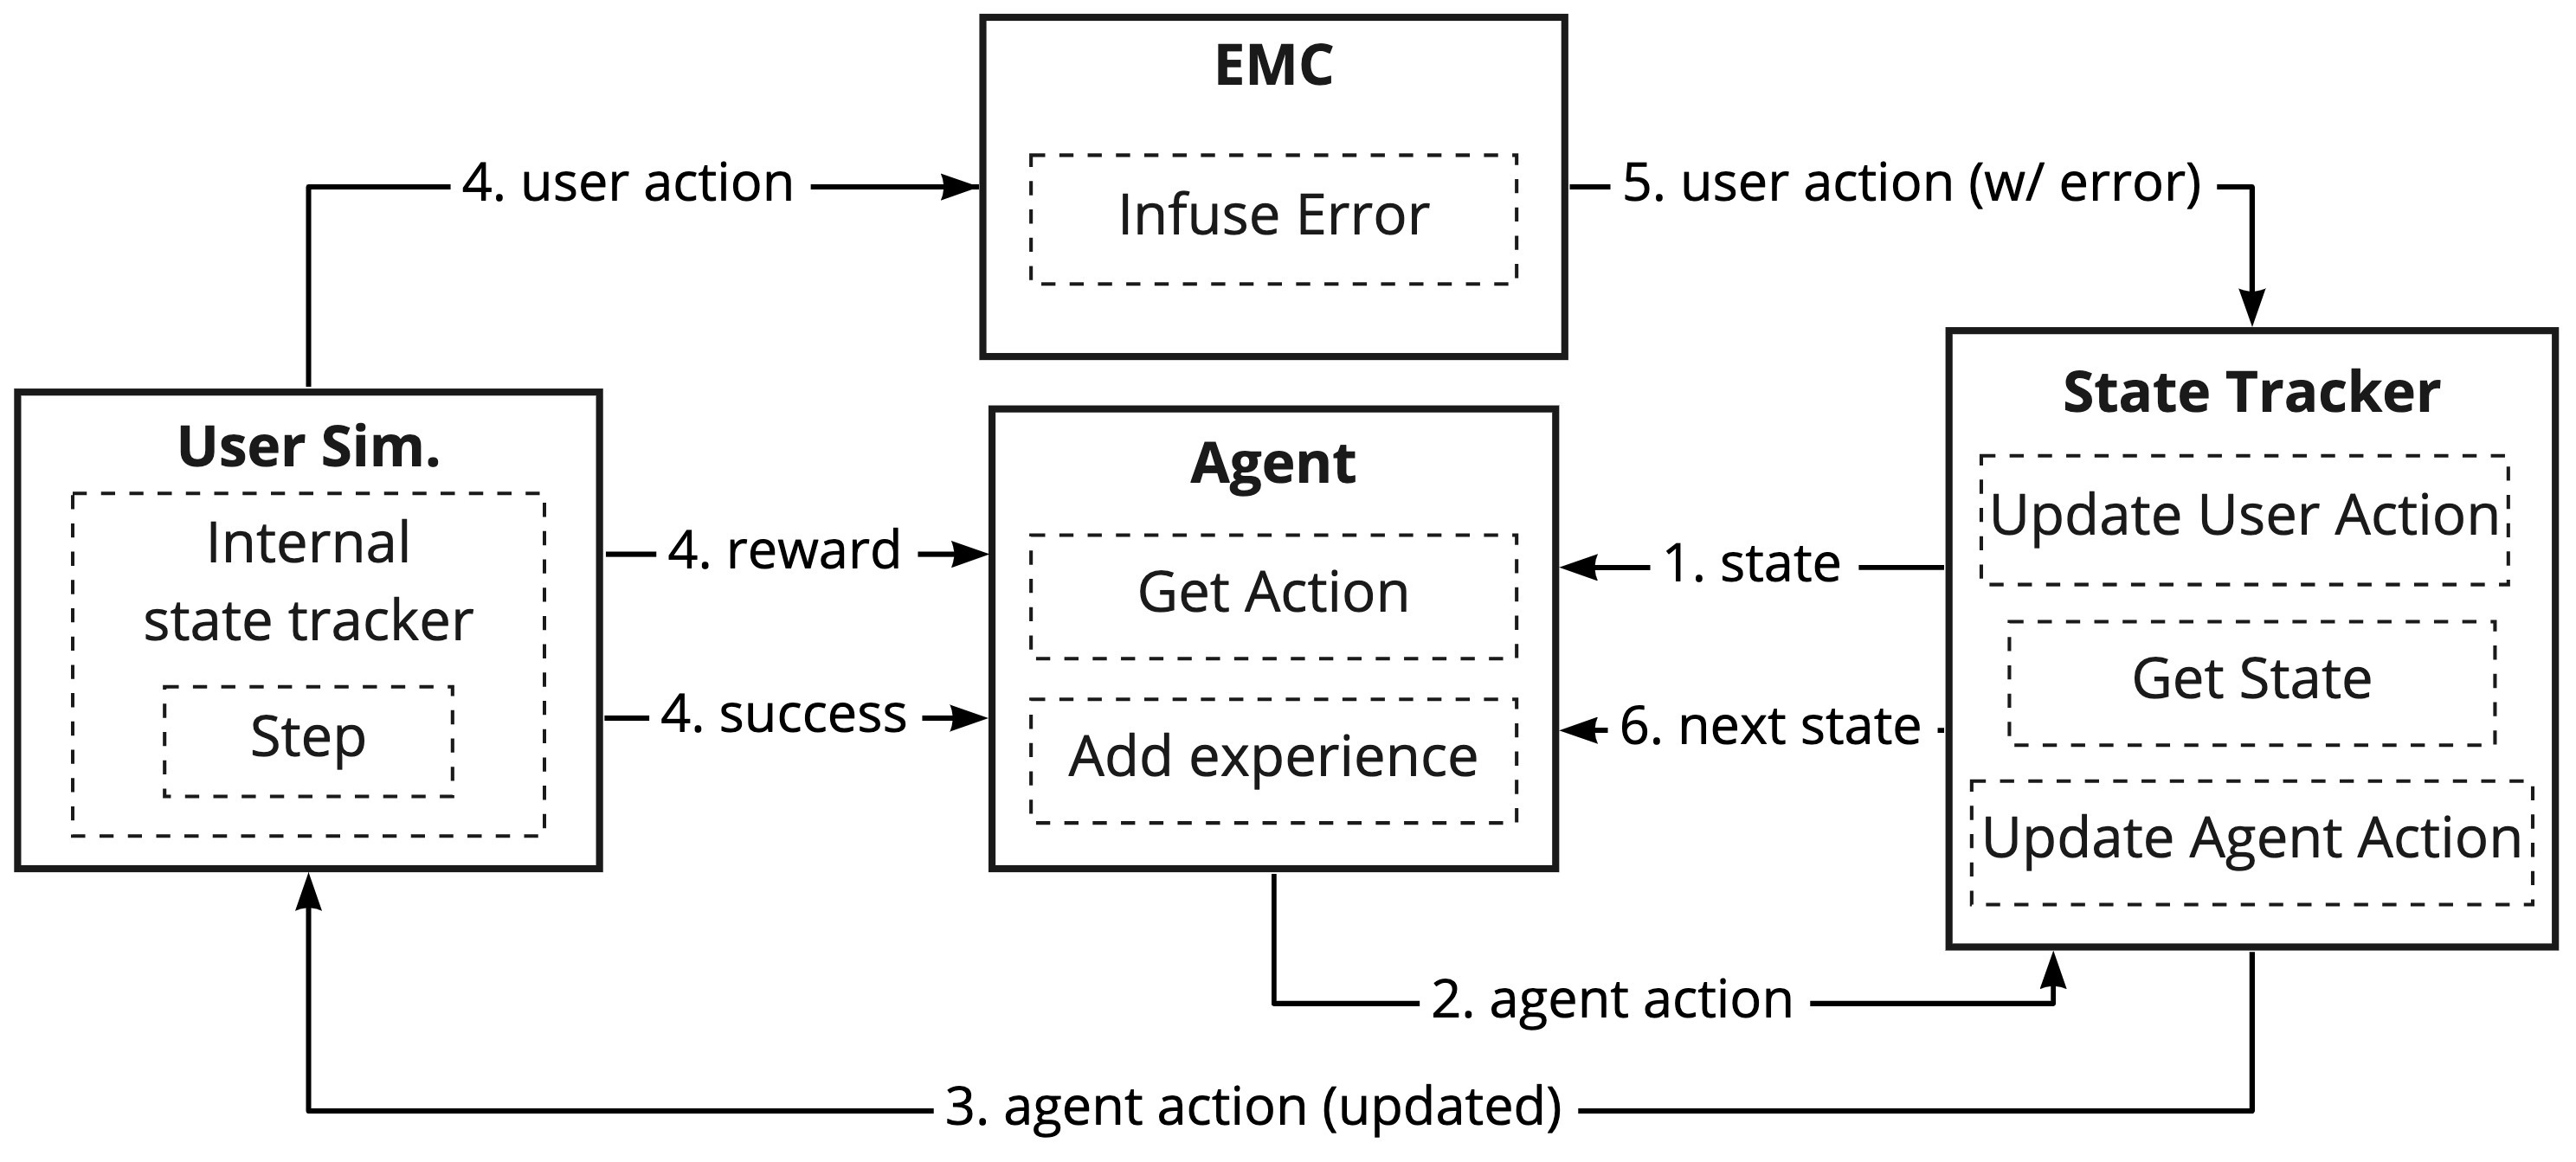
\includegraphics[scale=0.145]{thesis/chatbot/phuongphap/img/training.jpg}
    \caption{Vòng lặp huấn luyện - giai đoạn training}
    \label{fig:training}
\end{figure}

Mỗi một vòng thực hiện là một lượt đối thoại qua lại giữa người dùng
và tác nhân. Cụ thể:

\begin{itemize}
    \item \textbf{Bước 1:} Ta lấy ra \textit{state} - trạng thái
    hiện tại của hội thoại từ \textit{State Tracker} - bộ quản lý
    trạng thái hội thoại, trạng thái này có thể là trạng thái
    khởi tạo nếu như vừa bắt đầu hội thoại hoặc là trạng thái của
    toàn bộ cuộc hội thoại giữa người dùng và tác nhân. Trạng thái
    sau khi được lấy ra sẽ làm input (đầu vào) cho tác nhân ở
    bước tiếp theo.
    \item \textbf{Bước 2:} Tác nhân sau khi nhận được input từ
    bước trước sẽ sinh ra \textit{action} (hành động) và gửi ngược về
    lại bộ quản lý trạng thái hội thoại. Đồng thời ghi nhớ vào ký ức
    của nó. Hành động lúc này ở dạng thô, chưa kèm thông tin cụ thể.
    Nó sẽ được bộ quản lý trạng thái hội thoại cập nhật thông tin
    sau khi thực hiện truy vấn lên cơ sở dữ liệu cũng như cập nhật
    số lượt đã được thực hiện trong hội thoại. Đồng thời bộ quản lý
    trạng thái hội thoại cũng sẽ cập nhật lại trạng thái của hội thoại.
    \item \textbf{Bước 3:} Hành động sau khi được cập nhật đầy đủ
    thông tin sẽ được gửi cho bộ mô phỏng người dùng. Bộ mô phỏng
    người dùng sẽ dựa vào các luật đã được quy định trước để sinh ra
    hành động (có cấu trúc tương tự hành động của tác nhân ở
    bước trước), kèm theo \textit{reward} (điểm thưởng) và tín hiệu
    success (thành công) để giúp tác nhân có thể tự điều chỉnh
    hành vi để học. Ở đây, tác nhân cũng sẽ ghi lại toàn bộ vào
    ký ức của nó.
    \item \textbf{Bước 4:} Hành động của người dùng ở bước trước đó
    sẽ được đưa qua \textit{EMC} - bộ giả lập lỗi, trình bày cụ thể ở
    mục \ref{sec:emc}, mục đích là tạo ra các lỗi mà người dùng thật
    hay mắc phải, giúp tác nhân có hành vi chính xác và tự nhiên hơn
    khi chạy ở thực tế.
    \item \textbf{Bước 5:} Hành động ở bước trước sẽ tiếp tục được
    gửi đi đến bộ quản lý trạng thái hội thoại và được cập nhật
    thông tin cụ thể tương tự ở bước 2. Đồng thời bộ quản lý
    trạng thái hội thoại cũng cập nhật trạng thái của nó.
    \item \textbf{Bước 6:} Trạng thái tiếp theo được lấy từ bộ
    quản lý trạng thái hội thoại và quay lại giống bước 1.
\end{itemize}

Quá trình này sẽ được thực hiện liên tục cho đến khi tác nhân yêu cầu
kết thúc cuộc hội thoại sau khi nó nhận thấy đã hoàn thành yêu cầu
của người dùng hoặc khi số lượt hội thoại vượt quá mức ngưỡng quy định.

\subsubsection{Ví dụ}
Như trình bày ở trên, trong giai đoạn training, ta sẽ lấy ngẫu nhiên
một mục tiêu người dùng, được trình bày cụ thể ở mục
\ref{subsec:usergoal}, để làm mục tiêu cho bộ mô phỏng người dùng
trong suốt cuộc hội thoại. Xét một mẫu mục tiêu người dùng như sau:

\begin{itemize}
    \item Mục tiêu: yêu cầu thông tin sản phẩm
    \item Thông tin người dùng cung cấp trong hội thoại: tên sản phẩm
    \item Thông tin người dùng yêu cầu trong hội thoại: các màu
    khác nhau của sản phẩm
\end{itemize}

Giả sử, trạng thái chỉ chứa các ý định hành động hiện tại của
người dùng lần lượt là: hello, inform, request, reject, done.
Ta mã hóa về dạng one-hot vec-tơ để làm đầu vào cho mạng nơ-ron.
Quá trình huấn luyện trong giai đoạn training như sau:

\begin{itemize}
    \item Đầu tiên, bộ mô phỏng người dùng sẽ khởi tạo hành động
    đầu tiên trong hội thoại. Giả sử, nó tạo hành động như sau
    yêu cầu thông tin màu sắc và cung cấp tên sản phẩm
    (request(cost\_product), inform(name\_product)).
    Hành động này được đưa qua bộ giả lập lỗi. Giả sử, lỗi
    ngẫu nhiên được tạo là mất thông tin tên sản phẩm người dùng
    cung cấp. Hành động lúc này chỉ còn yêu cầu thông tin màu sắc
    (request(cost\_product)). Sau đó nó được gửi tới bộ quản lý
    trạng thái hội thoại. Bộ quản lý trạng thái hội thoại sẽ thêm
    thông tin số lượt thực hiện vào hành động của người dùng là 1
    để kiểm soát hội thoại kéo dài không quá số lượt cho phép (20).
    Đồng thời lấy trạng thái hiện tại của hội thoại gửi qua cho
    tác nhân là $[0\; 0\; 1\; 0\; 0]$. Quá trình được biểu diễn
    như hình \ref{fig:examtraining}.
\end{itemize}

\begin{figure}[ht!]
    \centering
    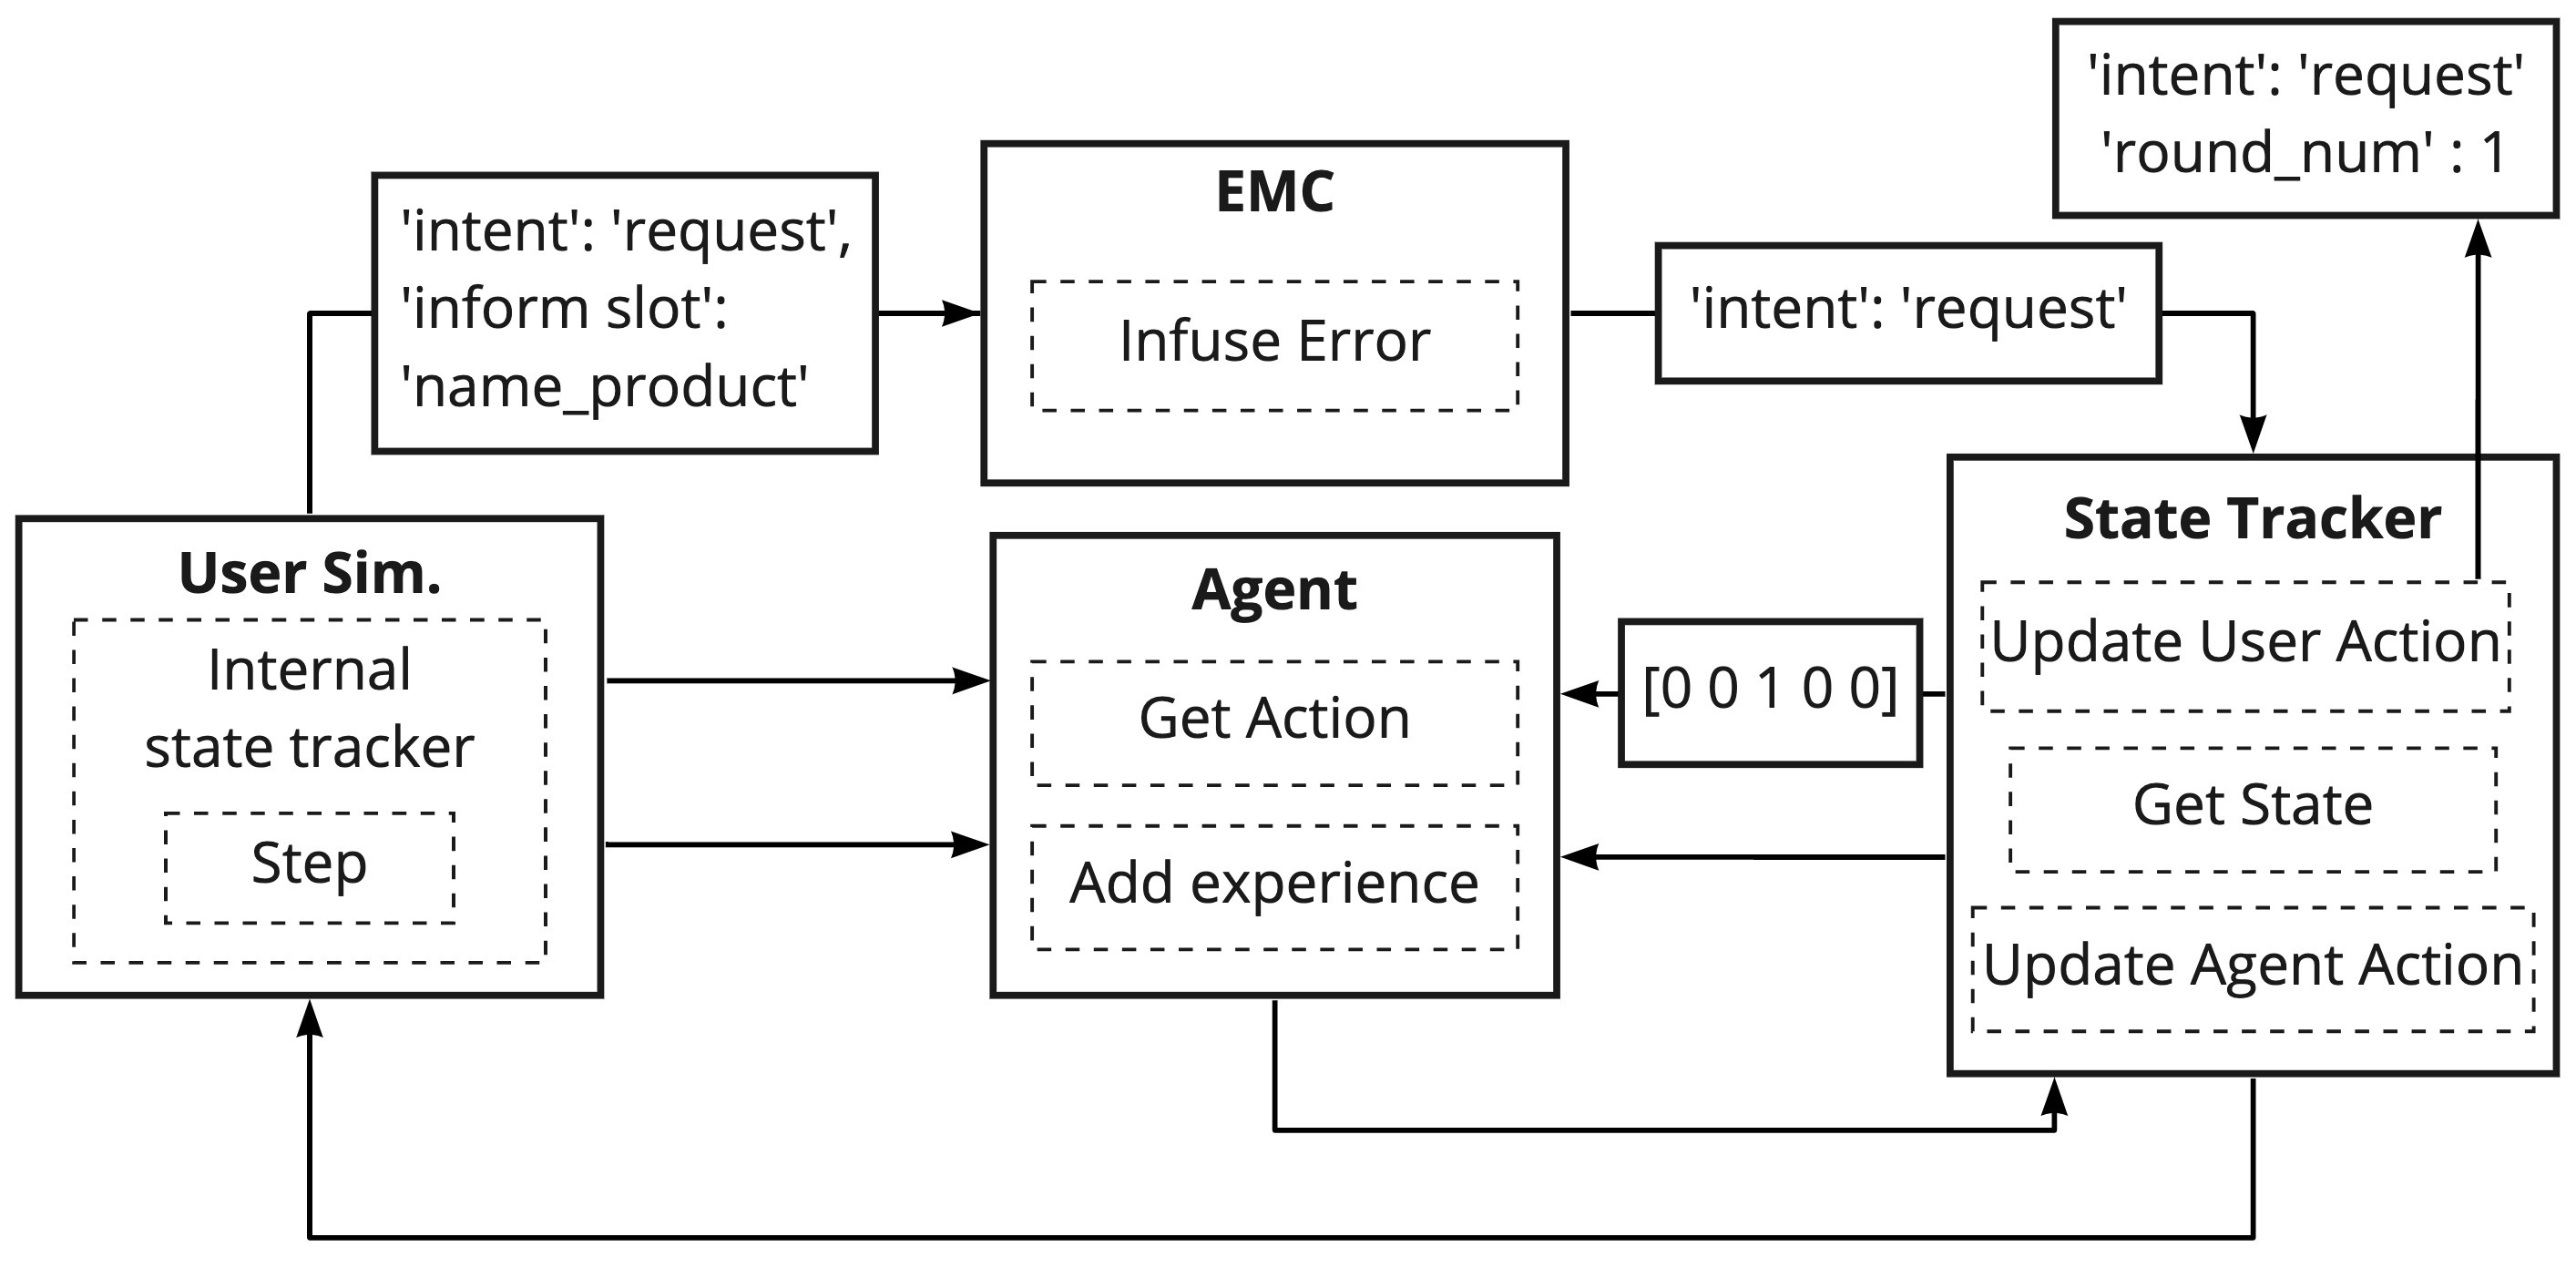
\includegraphics[scale=0.15]{thesis/chatbot/phuongphap/img/training_exam.jpg}
    \caption{Ví dụ quá trình huấn luyện bước 1 - giai đoạn training}
    \label{fig:examtraining}
\end{figure}

\begin{itemize}
    \item Tại đây, tác nhân sẽ đưa ra hành động có giá trị Q
    lớn nhất. Giả sử, ta có một mô hình với vộ trọng số như mục
    \ref{subsec:deepqlearning}, cho ra hành động kế tiếp là kết thúc
    hội thoại (done). Sau đó nó được gửi tới bộ quản lý trạng thái
    hội thoại. Tương tự, bộ quản lý trạng thái hội thoại sẽ thêm
    thông tin số lượt thực hiện vào hành động của tác nhân là 1 và
    gửi qua cho bộ mô phỏng người dùng. Quá trình được biểu diễn
    như hình \ref{fig:examtraining1}.
\end{itemize}

\begin{figure}[ht!]
    \centering
    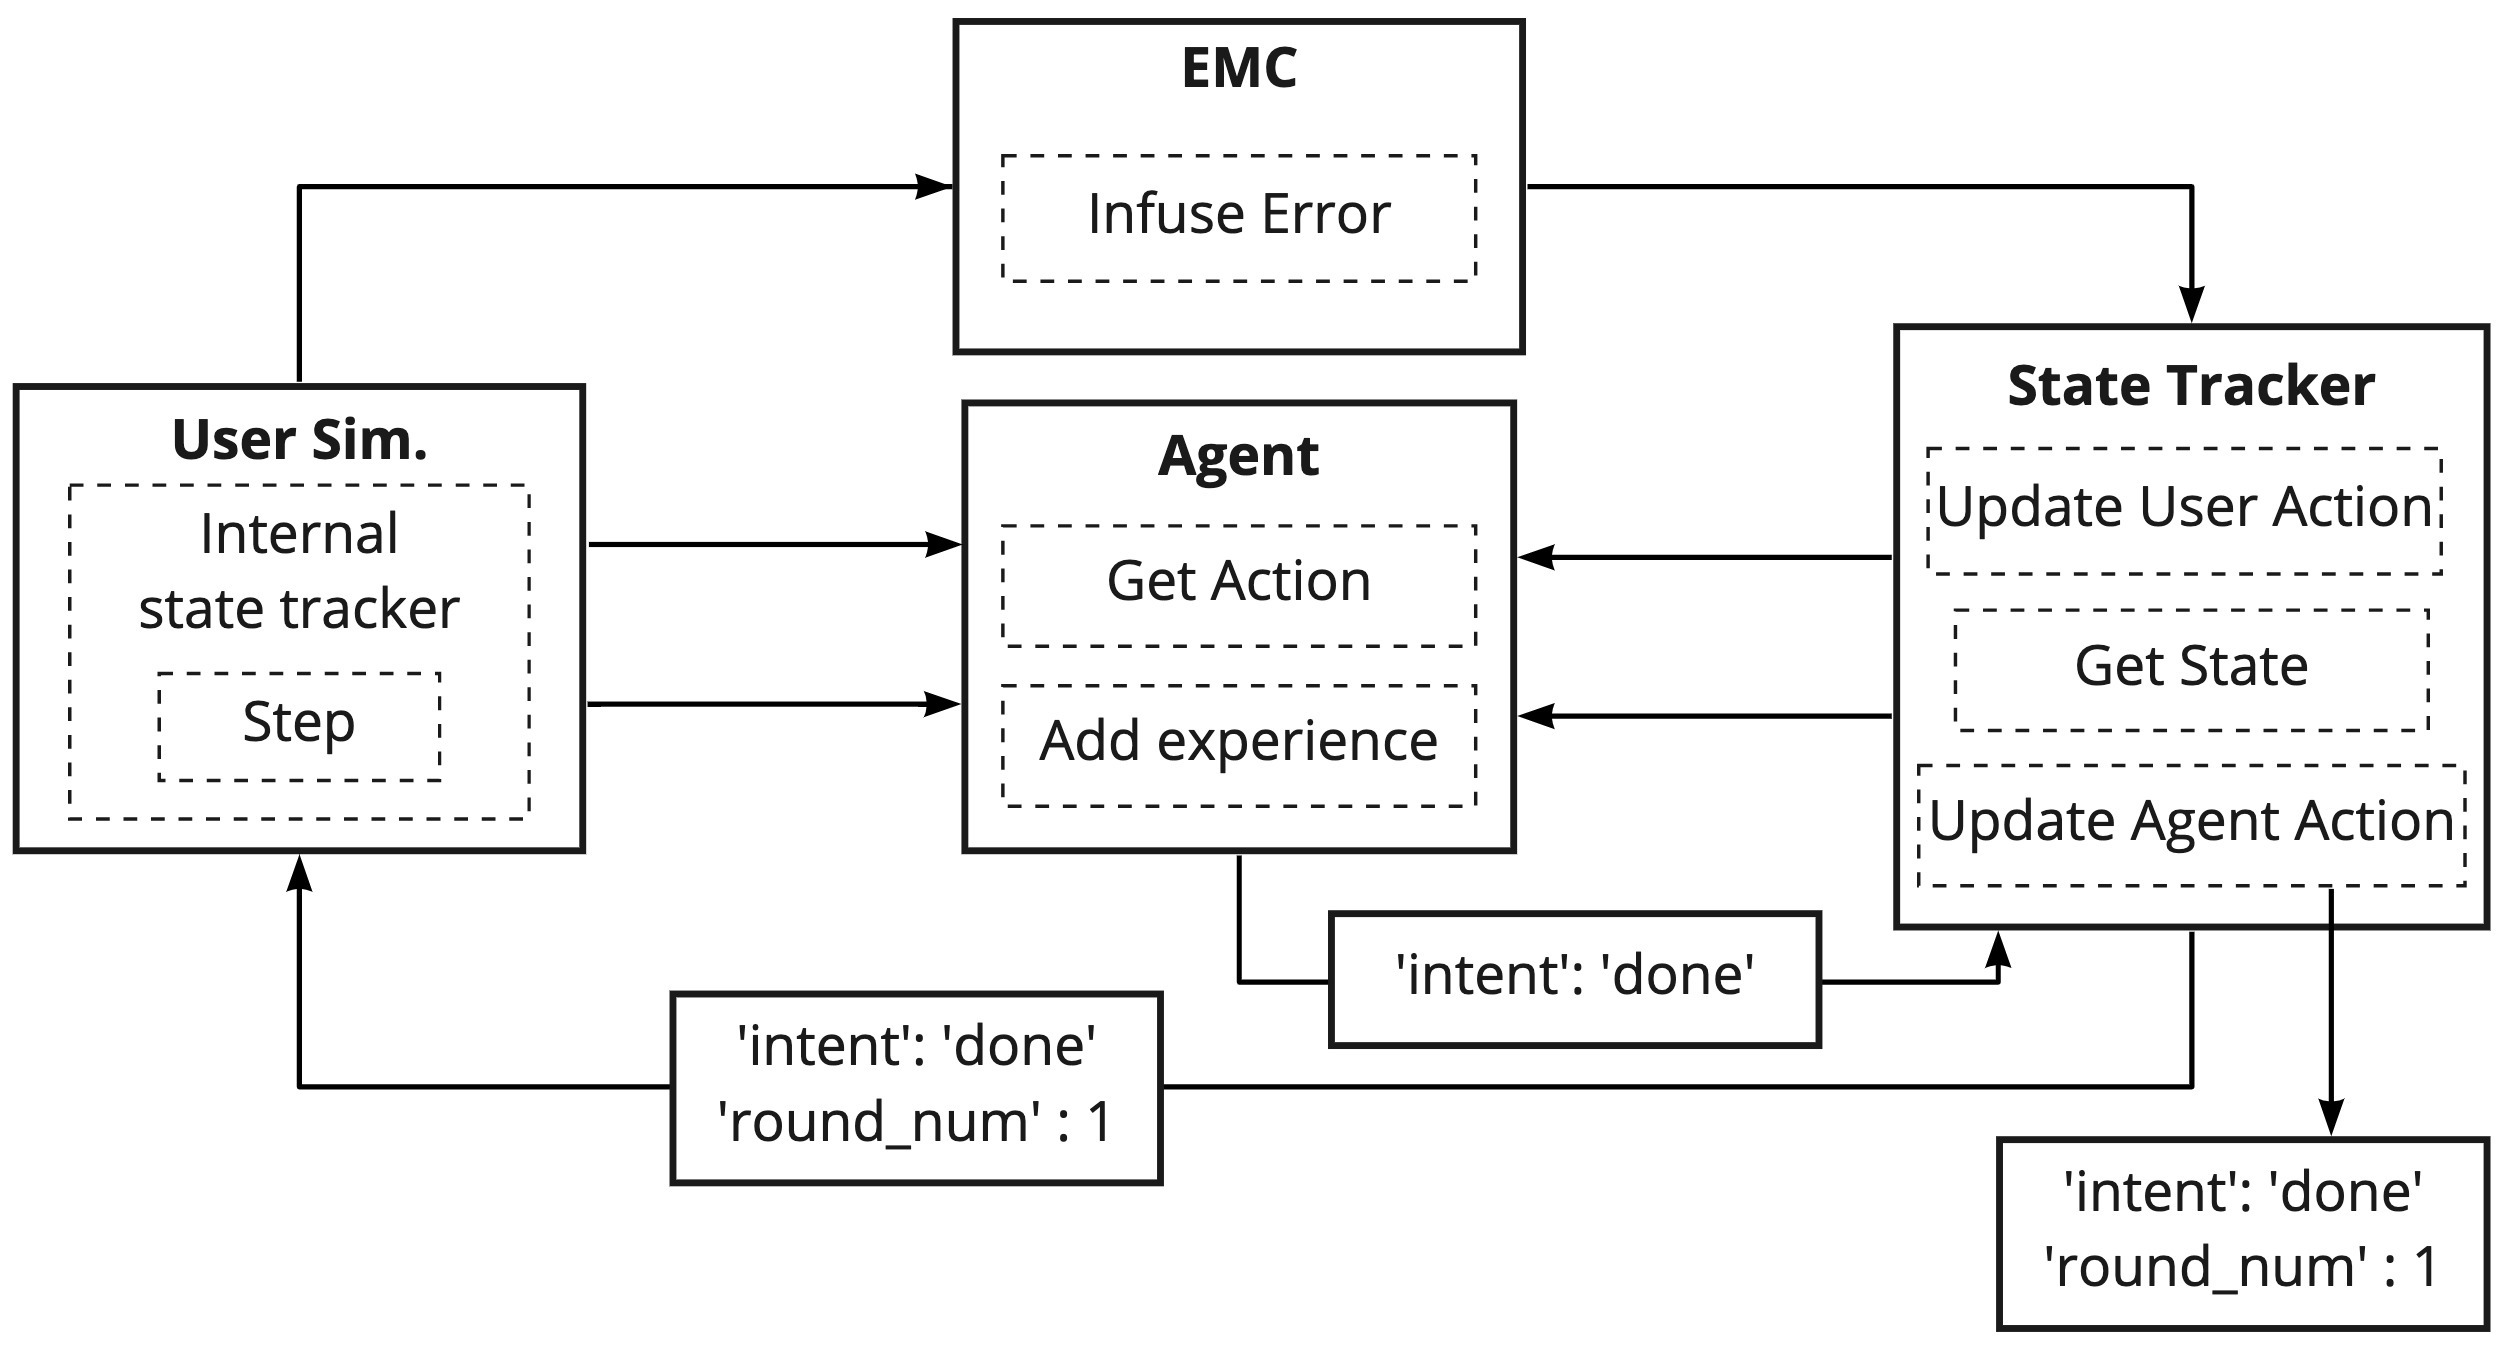
\includegraphics[scale=0.16]{thesis/chatbot/phuongphap/img/training_exam1.jpg}
    \caption{Ví dụ quá trình huấn luyện bước 2 - giai đoạn training}
    \label{fig:examtraining1}
\end{figure}

\begin{itemize}
    \item Hành động done là hành động kết thúc hội thoại của tác nhân
    mà nó chưa hoàn thành được mục tiêu cho người dùng. Vì vậy,
    với các luật quy định sẵn, bộ mô phỏng người dùng sẽ thực hiện
    hành động từ chối kết thúc hội thoại (reject), gửi tới bộ quản lý
    trạng thái hội thoại và gửi điểm thưởng là -10 cho tác nhân.
    Bộ quản lý trạng thái hội thoại sẽ thêm thông tin số lượt vào
    hành động của người dùng là 2. Cập nhật và lấy trạng thái hiện tại
    của hội thoại gửi qua cho tác nhân là $[0\; 0\; 0\; 1\; 0]$.
    Quá trình được biểu diễn như hình \ref{fig:examtraining2}.
\end{itemize}

\begin{figure}[ht!]
    \centering
    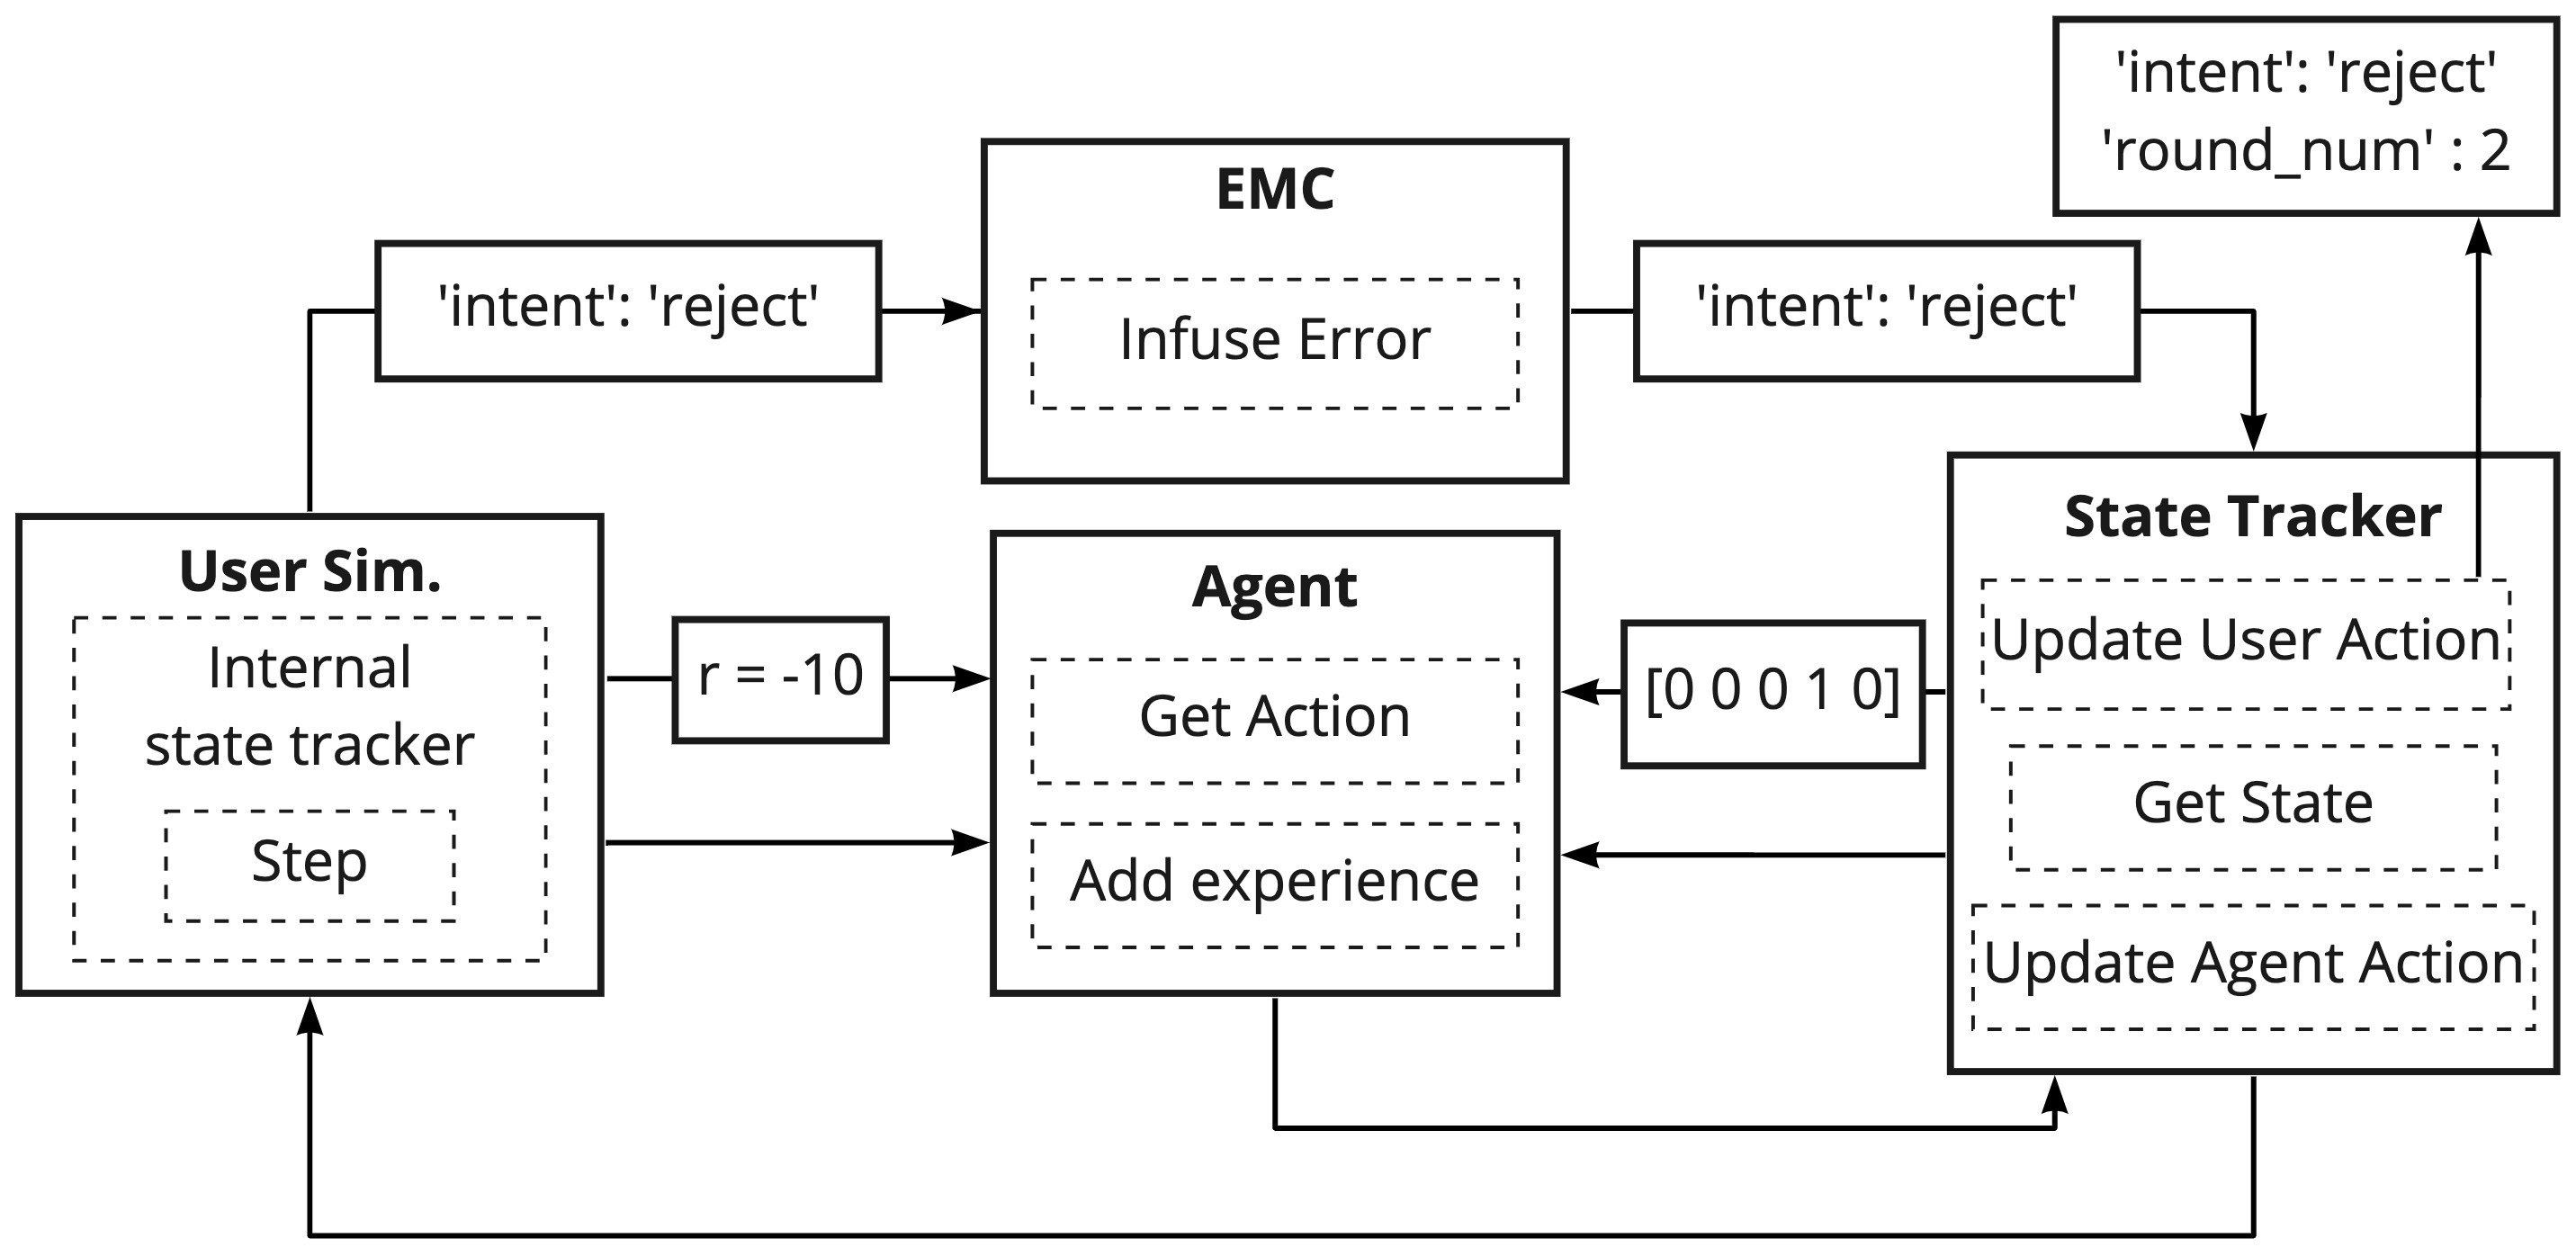
\includegraphics[scale=0.15]{thesis/chatbot/phuongphap/img/training_exam2.jpg}
    \caption{Ví dụ quá trình huấn luyện bước 3, 4 và 5 - giai đoạn training}
    \label{fig:examtraining2}
\end{figure}

Trạng thái hội thoại tại thời điểm này chính là trạng thái kế tiếp
của hành động trước đó (request(cost\_product),
inform(name\_product)) của người dùng.

Tại đây, chúng ta đã có đầy đủ thông tin:
\begin{itemize}
    \item State ($s$): trạng thái hiện tại khi người dùng yêu cầu
    thông tin và cung cấp tên sản phẩm (request(cost\_product),
    inform(name\_product)) là $[0\; 0\; 1\; 0\; 0]$.
    \item Next state ($s'$): trạng thái kế tiếp của người dùng
    sau khi tác nhân phản hồi yêu cầu kết thúc hội thoại (done)
    là $[0\; 0\; 0\; 1\; 0]$.
    \item Action ($a$): hành động tác nhân phản hồi tại
    trạng thái $s$ là done.
    \item Reward ($r_0$): phần thưởng cho hành động $a$ là -10.
\end{itemize}

Toàn bộ thông tin này được lưu vào bộ nhớ. Khác với giai đoạn warm-up.
Ta thực hiện việc huấn luyện như mô tả ở mục \ref{subsec:deepqlearning}
sau một số các hội thoại kết thúc được xác định trước.

\section{Vấn đề cần giải quyết}
Đề tài này có những vấn đề sau cần giải quyết:

\begin{itemize}
    \item Thu thập và chọn lọc các dữ liệu ban đầu vào cơ sở dữ liệu
    từ danh sách các thông tin sản phẩm của cửa hàng. Các dữ liệu về
    kích cỡ sản phẩm phù hợp với cơ thể người từ bảng kích cỡ của cửa hàng.
    \item Xác định các ý định của người dùng.
    \item Xây dựng được một bộ quản lý hội thoại cho Chatbot sao cho
    quá trình hội thoại được diễn ra tự nhiên và vẫn đáp ứng được
    nhu cầu tư vấn của người dùng.
    \item Xây dựng được một bộ phản hồi cho Chatbot sao cho các câu
    phản hồi tự nhiên và sát với con người nhất có thể, không tạo
    cảm giác quá rập khuôn hay cứng nhắc.
    \item Xây dựng được một trang web tích hợp các thành phần trong
    hệ thống thành Chatbot, có giao diện đơn giản, dễ sử dụng.
    \item Triển khai hệ thống và thu thập ý kiến đánh giá từ
    người dùng Chatbot.
\end{itemize}

\section{Khó khăn}
Trong quá trình giải quyết các vấn đề gặp phải các khó khăn sau:

\begin{itemize}
    \item Dữ liệu về bảng kích cỡ sản phẩm với số đo cơ thể người còn
    hạn chế, ảnh hưởng đến truy vấn tìm kiếm các thông tin phù hợp.
    \item Dữ liệu nhập bởi người dùng có thể có nhiều dạng khác nhau,
    việc chuẩn hóa thông tin đòi hỏi nhiều thời gian để nghiên cứu
    và thực hiện.
    \item Việc huấn luyện cho tác nhân gặp nhiều khó khăn ở bước đầu.
    Tác nhân phản hồi không hợp lý, cần nhiều thời gian để thử nghiệm
    trên các tập dữ liệu và điều chỉnh luật huấn luyện phù hợp.
\end{itemize}

\section{Giải pháp}
Để giải quyết các khó khăn đã nêu trên, đề xuất ra các giải pháp sau:

\begin{itemize}
    \item Nhờ sự giúp đỡ từ các cộng tác viên, và thông tin trực tiếp
    từ cửa hàng, cập nhật dữ liệu được đầy đủ và chính xác.
    \item Xây dựng bộ chuẩn hóa dữ liệu nhập vào theo giai đoạn,
    cải tiến từng phần dựa trên trải nghiệm thực tế.
    \item Phân tích, tìm hiểu rõ thuật toán và nguyên lý hoạt động
    của mô hình huấn luyện học tăng cường để tiến hành điều chỉnh các
    thông số, tập dữ liệu sao cho thích hợp và mang lại
    kết quả chính xác, đúng yêu cầu đặt ra.
\end{itemize}

\chapter{Công nghệ sử dụng}

\section{Ngôn ngữ lập trình}

\subsection{Python}
Python là một ngôn ngữ lập trình bậc cao cho các mục đích lập trình
đa năng, do Guido van Rossum tạo ra và lần đầu ra mắt vào năm 1991
và được phát triển trong một dự án mã nguồn mở. Python sử dụng
cơ chế cấp phát bộ nhớ động, hỗ trợ các phương thức lập trình như
lập trình hướng đối tượng, lập trình hàm.

Python được thiết kế với ưu điểm mạnh là dễ đọc, dễ học và dễ nhớ.
Python là ngôn ngữ có hình thức rất sáng sủa, cấu trúc rõ ràng,
thuận tiện cho người mới học lập trình và là ngôn ngữ lập trình
dễ học, được dùng rộng rãi trong phát triển trí tuệ nhân tạo.

Python hỗ trợ rất mạnh về Machine Learning, Deep Learning với các
thư viện như TensorFlow, Pytorch, Keras, ... Ngoài ra còn có các
thư viện hỗ trợ mạnh cho việc xử lý dữ liệu như là Pandas, Numpy,
Scipy, ...

Trong đề tài này sử dụng phiên bản Python 3.8 để hiện thực các
thành phần trong hệ thống.

\subsection{JavaScript}
JavaScript được tạo trong mười ngày bởi Brandan Eich, một nhân viên
của Netscape, vào tháng 9 năm 1995. JavaScript liên tục phát triển
kể từ đó. Chỉ sau 20 năm, nó từ một ngôn ngữ lập trình riêng trở thành
công cụ quan trọng nhất trên bộ công cụ của các chuyên viên lập trình web.

Một số đặc điểm của JavaScript:

\begin{itemize}
    \item Là một ngôn ngữ lập trình thông dịch.
    \item Không cần một compiler vì web browser có thể biên dịch nó
    bằng HTML.
    \item Dễ học và dễ sử dụng hơn các ngôn ngữ lập trình khác.
    \item Hoạt động trên nhiều trình duyệt, nền tảng.
\end{itemize}

JavaScript được dùng rộng rãi cho các trang web (phía người dùng)
cũng như phía máy chủ, cũng là một lý do khiến nó trở nên rất phổ biến.

\subsection{HTML}
HTML được tạo ra bởi Tim Berners-Lee, một nhà vật lý học của
trung tâm nghiên cứu CERN ở Thụy Sĩ. Hiện nay, HTML đã trở thành một
chuẩn Internet được tổ chức W3C (World Wide Web Consortium) vận hành
và phát triển.

HTML viết tắt của Hypertext Markup Language, tạm dịch là ngôn ngữ
đánh dấu siêu văn bản, là ngôn ngữ lập trình dùng để xây dựng và
cấu trúc lại các thành phần có trong Website. Nó có thể được trợ giúp
bởi các công nghệ như CSS và các ngôn ngữ kịch bản giống như JavaScript.

Một số đặc điểm của HTML:

\begin{itemize}
    \item Đây là một ngôn ngữ đơn giản rất dễ học và dễ sử dụng.
    \item Rất dễ dàng để trình bày hiệu quả với HTML vì nó có nhiều
    thẻ định dạng.
    \item Đây là một ngôn ngữ đánh dấu vì vậy có thể sử dụng nó một cách
    linh hoạt để thiết kế trang web cùng với văn bản.
    \item Hoạt động trên nhiều trình duyệt, nền tảng.
\end{itemize}

\subsection{CSS}
CSS là chữ viết tắt của Cascading Style Sheets, nó là một ngôn ngữ
được sử dụng để tìm và định dạng lại các phần tử được tạo ra bởi các
ngôn ngữ đánh dấu (HTML). Nói ngắn gọn hơn là ngôn ngữ tạo phong cách
cho trang web. Nếu HTML đóng vai trò định dạng các phần tử trên
website như việc tạo ra các đoạn văn bản, các tiêu đề, bảng, ... thì
CSS sẽ giúp chúng ta có thể thêm style vào các phần tử HTML đó như
đổi bố cục, màu sắc trang, đổi màu chữ, font chữ, thay đổi cấu trúc, ...

CSS được phát triển bởi W3C (World Wide Web Consortium) vào năm 1996,
vì HTML không được thiết kế để gắn tag để giúp định dạng trang web.

Mối tương quan giữa HTML và CSS rất mật thiết. HTML là ngôn ngữ markup
(nền tảng của site) và CSS định hình phong cách (tất cả những gì tạo
nên giao diện website), chúng là không thể tách rời.

\subsection{JSON}
JSON là chữ viết tắt của Javascript Object Notation, đây là một dạng
dữ liệu tuân theo một quy luật nhất định mà hầu hết các ngôn ngữ
lập trình hiện nay đều có thể đọc được.

JSON sử dụng cú pháp Javascript, nhưng định dạng JSON chỉ văn bản như
XML. Ta có thể sử dụng lưu nó vào một tệp (file), một bản ghi (record)
trong cơ sở dữ liệu rất dễ dàng.

JSON có định dạng đơn giản, là một dạng trao đổi dữ liệu trọng lượng
nhẹ (lightweight data-interchange format), xử lý nhanh, dễ hiểu,
dễ dàng sử dụng hơn XML rất nhiều nên tính ứng dụng của nó hiện nay
rất là phổ biến, trong tương lai tới, các ứng dụng sẽ sử dụng JSON
là đa số.

\section{Nền tảng và thư viện}

\subsection{Pandas}
Pandas là một thư viện phần mềm được viết cho ngôn ngữ lập trình
Python để thao tác và phân tích dữ liệu. Với Pandas, người dùng
có thể dễ dàng tạo ra các bảng dữ liệu (Dataframe) và thực hiện
các phép truy vấn, thống kê trên nó, cho phép đọc/ghi các
định dạng file một cách dễ dàng.

\subsection{TensorFlow}
TensorFlow là một thư viện phần mềm mã nguồn mở dành cho máy học
trong nhiều loại hình tác vụ nhận thức và hiểu ngôn ngữ.

TensorFlow nguyên thủy được phát triển bởi đội Google Brain cho
mục đích nghiên cứu và sản xuất của Google và sau đó được phát hành
theo giấy phép mã nguồn mở Apache 2.0.

TensorFlow tích hợp sẵn rất nhiều các thư viện Machine Learning,
Deep Learning, có khả năng tương thích và mở rộng tốt. Trong đề tài
này, sử dụng nó trong việc xây dựng mạng Deep Q-Learning.

\subsection{Keras}
Keras là một thư viện mạng nơ ron được viết bằng Python năm 2015 bởi
một kỹ sư Deep Learning của Google. Ta có thể kết hợp Keras với các
thư viện Deep Learning. Keras được phát triển với trọng tâm là
cho phép thử nghiệm nhanh, việc thử nghiệm nhanh đôi khi sẽ mang lại
kết quả nghiên cứu tốt. Trong đề tài này, sử dụng Keras trong việc
xây dựng mô hình Deep Q-Learning.

\subsection{Eel}
Eel là một thư viện Python nhỏ để tạo các ứng dụng GUI ngoại tuyến
HTML/JS đơn giản, với toàn quyền truy cập vào các khả năng và
thư viện Python. Eel lưu trữ một máy chủ web cục bộ, sau đó cho phép
chú thích các hàm bằng Python để chúng có thể được gọi từ Javascript
và ngược lại. Eel được thiết kế để giảm bớt rắc rối khi viết các
ứng dụng GUI ngắn và đơn giản.

\section{Công cụ}

\subsection{Google Colab}
Colaboratory hay còn gọi là Google Colab, là một sản phẩm từ Google
Research, nó cho phép chạy các dòng code python thông qua
trình duyệt, đặc biệt phù hợp với Data analysis, machine learning
và giáo dục. Colab không cần yêu cầu cài đặt hay cấu hình máy tính,
mọi thứ có thể chạy thông qua trình duyệt, có thể sử dụng tài nguyên
máy tính từ CPU tốc độ cao và cả GPUs và cả TPUs đều được cung cấp.

\chapter{Hiện thực hệ thống}

\section{Dữ liệu}
\label{sec:database}
Dưới sự hỗ trợ của một cửa hàng thời trang thực tế (Thời trang Hume),
đề tài thực hiện việc chuẩn hóa và gán nhãn cho các dữ liệu về
sản phẩm, phục vụ cho nhu cầu tư vấn của người dùng. Ngoài ra, đề tài
còn thu thập và tổng hợp một số loại dữ liệu khác phục vụ cho các
mục đích khác nhau.

\subsection{Dữ liệu sản phẩm}
\label{subsec:productdb}
Dữ liệu sản phẩm này chứa các thông tin sản phẩm dùng để tư vấn,
tìm kiếm cho khách hàng một sản phẩm phù hợp với yêu cầu, một bản ghi
trong cơ sở dữ liệu tương ứng với một sản phẩm. Mỗi trường thông tin
của sản phẩm có thể có các định dạng khác nhau. Cụ thể:

\begin{itemize}
    \item \textbf{name\_product:} tên của sản phẩm, có thể có nhiều
    alias của tên sản phẩm trong cơ sở dữ liệu sản phẩm, thuộc kiểu
    dữ liệu chuỗi ký tự (string).
    \item \textbf{size\_product:} kích cỡ của sản phẩm, có thể có
    nhiều alias của kích cỡ sản phẩm trong cơ sở dữ liệu sản phẩm,
    thuộc kiểu dữ liệu chuỗi ký tự (string).
    \item \textbf{color\_product:} màu sắc của sản phẩm, có thể có
    nhiều alias của màu sắc sản phẩm trong cơ sở dữ liệu sản phẩm,
    thuộc kiểu dữ liệu chuỗi ký tự (string).
    \item \textbf{material\_product:} chất liệu của sản phẩm, có thể
    có nhiều alias của chất liệu sản phẩm trong cơ sở dữ liệu
    sản phẩm, thuộc kiểu dữ liệu chuỗi ký tự (string).
    \item \textbf{cost\_product:} đơn giá của sản phẩm, có thể có
    nhiều alias của đơn giá sản phẩm trong cơ sở dữ liệu sản phẩm,
    thuộc kiểu dữ liệu chuỗi ký tự (string).
    \item \textbf{amount\_product:} số lượng sản phẩm hiện tại,
    có thể có nhiều alias của số lượng sản phẩm trong cơ sở dữ liệu
    sản phẩm, thuộc kiểu dữ liệu số (int).
\end{itemize}

Bản ghi mẫu của dữ liệu sản phẩm như ví dụ \ref{exam:productrecord}.

\renewcommand{\textboxenvname}{Ví dụ}
\begin{textbox}[exam:productrecord]{Một bản ghi của dữ liệu sản phẩm}
\begin{Verbatim}[breaklines=true, breakanywhere=true]
{
    "name_product": "set trắng cổ nơ",
    "size_product": "M",
    "color_product": "None",
    "cost_product": "260",
    "material_product": "vải cao cấp, mặc mát",
    "amount_product": 10
}
\end{Verbatim}
\end{textbox}

\subsection{Dữ liệu kích cỡ}
\label{subsec:sizedb}
Dữ liệu kích cỡ này chứa các thông tin về kích thước dùng để tư vấn,
tìm kiếm cho khách hàng một kích cỡ sản phẩm phù hợp với số đo cơ thể,
một bản ghi trong cơ sở dữ liệu tương ứng với một bảng kích thước.
Mỗi trường thông tin của dữ liệu có thể có các định dạng khác nhau.
Các giá trị của cùng một thông tin có cùng một đơn vị. Cụ thể:

\begin{itemize}
    \item \textbf{size\_customer:} kích cỡ sản phẩm phù hợp với
    khách hàng, có thể có nhiều alias của kích cỡ sản phẩm trong
    cơ sở dữ liệu kích cỡ, thuộc kiểu dữ liệu chuỗi ký tự (string).
    \item \textbf{waist\_customer:} số đo vòng eo của cơ thể, có thể
    có nhiều alias của số đo vòng eo trong cơ sở dữ liệu kích cỡ,
    thuộc kiểu dữ liệu chuỗi ký tự (string), đơn vị là centimet (cm).
    \item \textbf{height\_customer:} số đo chiều cao của cơ thể,
    có thể có nhiều alias của số đo chiều cao trong cơ sở dữ liệu
    kích cỡ, thuộc kiểu dữ liệu chuỗi ký tự (string), đơn vị là
    centimet (cm).
    \item \textbf{weight\_customer:} số đo cân nặng của cơ thể,
    có thể có nhiều alias của số đo cân nặng trong cơ sở dữ liệu
    kích cỡ, thuộc kiểu dữ liệu chuỗi ký tự (string), đơn vị là
    kilogram (kg).
\end{itemize}

Bản ghi mẫu của dữ liệu kích cỡ như ví dụ \ref{exam:sizerecord}.

\renewcommand{\textboxenvname}{Ví dụ}
\begin{textbox}[exam:sizerecord]{Một bản ghi của dữ liệu kích cỡ}
\begin{Verbatim}[breaklines=true, breakanywhere=true]
{
    "size_customer": "S",
    "waist_customer": "65",
    "height_customer": "164",
    "weight_customer": "50"
}
\end{Verbatim}
\end{textbox}

\subsection{Từ điển thông tin sản phẩm}
Từ điển (Dictionary) của thông tin sản phẩm chứa tất cả các giá trị
có thể có của từng thông tin sản phẩm (như mô tả ở mục
\ref{subsec:productdb}). Dữ liệu được sử dụng để tạo ra các
\textit{User Goal} (mục tiêu người dùng), phục vụ cho việc
huấn luyện. Ngoài ra được sử dụng bởi \textit{EMC} (bộ giả lập lỗi),
bộ tạo ra các lỗi ngẫu nhiên của người dùng. Mỗi trường thông tin
có định dạng danh sách (array). Được biểu diễn rút gọn như ví dụ
\ref{exam:dictproduct}.

\renewcommand{\textboxenvname}{Ví dụ}
\begin{textbox}[exam:dictproduct]{Từ điển thông tin sản phẩm}
\begin{Verbatim}[breaklines=true, breakanywhere=true]
{
    "name_product": ["đầm nude cổ vest dáng dài", "đầm sơ mi carô", "set hồng vest váy ngắn", "đầm nude lưới tay phồng", ...],
    "size_product": ["S", "M", "L", ...],
    "color_product": ["nude", "carô xanh", "hồng", "xanh", ...],
    "cost_product": ["280", "210", "260", "238", "195", "350", ...],
    "material_product": ["vải cao cấp, mặc mát", ...],
    "amount_product": ["2", "5", "hai", "9", "ba", "4", "3", "6", ...]
}
\end{Verbatim}
\end{textbox}

\subsection{Từ điển dữ liệu kích cỡ}
Từ điển (Dictionary) của bảng dữ liệu kích cỡ chứa tất cả các giá trị
có thể có của từng trường thông tin trong dữ liệu kích cỡ (như mô tả
ở mục \ref{subsec:sizedb}). Dữ liệu được sử dụng để tạo ra các
\textit{User Goal} (mục tiêu người dùng), phục vụ cho việc huấn luyện.
Ngoài ra được sử dụng bởi \textit{EMC} (bộ giả lập lỗi), bộ tạo ra
các lỗi ngẫu nhiên của người dùng. Mỗi trường thông tin có định dạng
danh sách (array). Được biểu diễn rút gọn như ví dụ \ref{exam:dictsize}.

\renewcommand{\textboxenvname}{Ví dụ}
\begin{textbox}[exam:dictsize]{Từ điển dữ liệu kích cỡ}
\begin{Verbatim}[breaklines=true, breakanywhere=true]
{
    "size_customer": ["L", "S", "M"],
    "waist_customer": ["anything", "66", "73", "68", "63", "58", ...],
    "height_customer": ["163", "159", "166", "150", "anything", "155", "165", "156", ...],
    "weight_customer": ["56", "45", "47", "46", "57", "48", "41", "52", "anything", ...]
}
\end{Verbatim}
\end{textbox}

\subsection{Mục tiêu người dùng (User Goal)}
\label{subsec:usergoal}
Mục tiêu người dùng (User Goal) chứa danh sách các trường hợp biểu diễn
mục tiêu có thể có của người dùng. Dữ liệu được sử dụng bởi bộ mô phỏng
người dùng sử dụng như mục tiêu thật của người dùng, phục vụ cho
quá trình huấn luyện. Mỗi \textit{goal} chỉ chứa cho một mục tiêu
xuyên suốt cuộc hội thoại. Cấu trúc cho một \textit{goal} như sau:

\begin{itemize}
    \item \textbf{intent:} mục tiêu chính của người dùng trong cuộc
    hội thoại, kiểu dữ liệu chuỗi ký tự (string). Các mục tiêu khi
    tham gia hội thoại của người dùng có thể có là:
    \begin{itemize}
        \item \textbf{request:} yêu cầu thông tin sản phẩm, hoặc
        tư vấn kích cỡ sản phẩm cho khách hàng
        \item \textbf{order:} mục tiêu đặt hàng sản phẩm của khách hàng
    \end{itemize}
    \item \textbf{inform\_slots:} chứa tất cả các thông tin cần
    thông báo cho tác nhân trong suốt cuộc hội thoại. Các thông tin
    cần thông báo có cấu trúc <tên thông tin>: <giá trị của thông tin>.
    Trong đó:
    \begin{itemize}
        \item \textbf{<tên thông tin>:} tên thông tin là một trong các
        trường thông tin đã được định nghĩa ở mục \ref{subsec:productdb}
        và \ref{subsec:sizedb}.
        \item \textbf{<giá trị của thông tin>:} giá trị của thông tin
        này có thể nằm trong bộ từ điển của nó hoặc không.
    \end{itemize}
    \item \textbf{request\_slots:} chứa tất cả các thông tin yêu cầu
    tác nhân cung cấp cho đến khi kết thúc cuộc hội thoại. Các
    thông tin yêu cầu có cấu trúc <tên thông tin>: \enquote{UNK}. Trong đó:
    \begin{itemize}
        \item \textbf{<tên thông tin>:} tên thông tin là một trong
        các trường thông tin đã được định nghĩa ở mục
        \ref{subsec:productdb} và \ref{subsec:sizedb}.
        \item \textbf{"UNK":} giá trị mặc định, có nghĩa \enquote{chưa biết},
        cần được thông báo/ điền vào từ tác nhân.
    \end{itemize}
\end{itemize}

Bản ghi mẫu của mục tiêu người dùng như ví dụ \ref{exam:goalrecord}.

\renewcommand{\textboxenvname}{Ví dụ}
\begin{textbox}[exam:goalrecord]{Một bản ghi của mục tiêu người dùng}
\begin{Verbatim}[breaklines=true, breakanywhere=true]
{
    "intent": "request",
    "inform_slots": {
        "name_product": "set dây kèm quần",
        "amount_product": "4",
        "color_product": "đen viền",
        "waist_customer": "63",
        "height_customer": "158",
        "weight_customer": "59"
    },
    "request_slots": {
        "size_product": "UNK",
        "material_product": "UNK",
        "cost_product": "UNK"
    }
}
\end{Verbatim}
\end{textbox}

\subsection{Hội thoại (Dialog)}
Dữ liệu hội thoại (Dialog) chứa danh sách các cuộc hội thoại tư vấn,
như mô tả ở mục \ref{subsubsec:dialog}. Dữ liệu được sử dụng cho
giai đoạn khởi động. Mỗi \textit{dialog} mô tả quá trình hội thoại
tư vấn diễn ra như trong thực tế, chứa danh sách các hành động lần lượt
là của người dùng và tác nhân, mỗi hành động có cấu trúc như sau:

\begin{itemize}
    \item \textbf{speaker:} mô tả lượt hành động do người dùng hay
    tác nhân thực hiện, kiểu dữ liệu là chuỗi ký tự (string).
    \item \textbf{intent:} ý định hành động của người dùng hoặc tác nhân
    trong lượt thoại hiện tại, kiểu dữ liệu chuỗi ký tự (string).
    Các mục tiêu có thể có được mô tả ở bảng \ref{tab:userintent}.
    \item \textbf{inform\_slots:} chứa các thông tin cần thông báo trong
    lượt thoại hiện tại. Các thông tin cần thông báo có cấu trúc
    <tên thông tin>: <giá trị của thông tin>. Trong đó:
    \begin{itemize}
        \item \textbf{<tên thông tin>:} tên thông tin là một trong các
        trường thông tin đã được định nghĩa ở mục \ref{subsec:productdb}
        và \ref{subsec:sizedb}.
        \item \textbf{<giá trị của thông tin>:} giá trị của thông tin
        này có thể nằm trong bộ từ điển của nó hoặc không.
    \end{itemize}
    \item \textbf{request\_slots:} chứa các thông tin yêu cầu đối phương
    cung cấp trong lượt thoại hiện tại. Trường thông tin yêu cầu này là
    danh sách các thông tin có kiểu dữ liệu là chuỗi ký tự (string).
    \begin{itemize}
        \item \textbf{<tên thông tin>:} tên thông tin là một trong các
        trường thông tin đã được định nghĩa ở mục \ref{subsec:productdb}
        và \ref{subsec:sizedb}.
    \end{itemize}
\end{itemize}

Bản ghi mẫu của hội thoại như ví dụ \ref{exam:dialogrecord}.

\renewcommand{\textboxenvname}{Ví dụ}
\begin{textbox}[exam:dialogrecord]{Một đoạn hội thoại}
\begin{Verbatim}[breaklines=true, breakanywhere=true]
[
    {"speaker": "user", "intent": "request", "inform_slots": {}, "request_slots": ["cost_product"]},
    {"speaker": "agent", "intent": "request", "inform_slots": {}, "request_slots": ["name_product"]},
    {"speaker": "user", "intent": "inform", "inform_slots": {"name_product": "đầm body vest"}, "request_slots": []},
    {"speaker": "agent", "intent": "inform", "inform_slots": {"cost_product": "260"}, "request_slots": []},
    {"speaker": "user", "intent": "ok", "inform_slots": {}, "request_slots": []},
    {"speaker": "agent", "intent": "match_found", "inform_slots": {}, "request_slots": []},
    {"speaker": "user", "intent": "ok", "inform_slots": {}, "request_slots": []},
    {"speaker": "agent", "intent": "done", "inform_slots": {}, "request_slots": []},
    {"speaker": "user", "intent": "done", "inform_slots": {}, "request_slots": []}
]
\end{Verbatim}
\end{textbox}

\section{Bộ xử lý phản hồi người dùng}
Do giới hạn của đề tài, trong luận án này không xử lý ngôn ngữ tự nhiên
cho các câu phản hồi của người dùng. Tuy nhiên, hệ thống có thể tích hợp
với bộ xử lý ngôn ngữ tự nhiên khác. Trong bộ xử lý phản hồi người dùng
này, hệ thống sẽ tiến hành xử lý các thông tin nhập vào từ giao diện
hệ thống Chabot hoặc kết quả trả về từ bộ xử lý ngôn ngữ tự nhiên
bên ngoài thành một cấu trúc đồng nhất để sử dụng trong lõi hệ thống,
lõi hệ thống như mô tả ở hình \ref{fig:chatbotapp}. Các hành động được
biểu diễn như cấu trúc \ref{struct:action}.

\renewcommand{\textboxenvname}{Cấu trúc}
\begin{textbox}[struct:action]{Cấu trúc cho một hành động}
\begin{Verbatim}[breaklines=true, breakanywhere=true]
{
    "intent": <value 1>,
    "inform_slots": <value 2>,
    "request_slots": <value 3>
}
\end{Verbatim}
\end{textbox}

Trong đó:

\begin{itemize}
    \item \textbf{<value 1>}: chứa ý định người dùng, các giá trị
    hợp lệ được mô tả trong bảng \ref{tab:userintent}
    \item \textbf{<value 2>}: là một dictionary (kiểu dữ liệu của
    Python), có cấu trúc key:value, với key là tên thông tin
    cung cấp, các trường thông tin được định nghĩa ở mục
    \ref{subsec:productdb} và \ref{subsec:sizedb}, value là giá trị
    của thông tin
    \item \textbf{<value 3>}: là một dictionary, có cấu trúc
    key:value, với key là tên thông tin yêu cầu, các trường
    thông tin được định nghĩa ở mục \ref{subsec:productdb} và
    \ref{subsec:sizedb}, value có giá trị mặc định là
    chuỗi kí tự \enquote{UNK}.
\end{itemize}

\begin{table}[!ht]
\caption{Các ý định hành động của người dùng}
\label{tab:userintent}
\centering
\begin{tabular}{|C{1cm}|C{1.5cm}|L{11cm}|}
\hline
\textbf{STT} & \textbf{Ý định} & \textbf{Mô tả} \\ % inserts table %heading
\hline
1 &
hello &
Ý định khi người dùng thực hiện các câu chào, hỏi thăm với tác nhân \\
\hline
2 &
inform &
Ý định khi người dùng cần thông báo thông tin đến cho tác nhân \\
\hline
3 &
request &
Ý định khi người dùng yêu cầu tác nhân cung cấp thông tin \\
\hline
4 &
order &
Ý định khi người dùng muốn đặt hàng sản phẩm \\
\hline
5 &
ok &
Ý định khi người dùng thể hiện ý đồng tình, chỉ cho tác nhân
biết rằng nó đã làm điều gì đó tốt, đúng hoặc người dùng đã
sẵn sàng kết thúc cuộc trò chuyện \\
\hline
6 &
reject &
Ý định khi người dùng thể hiện ý phản đối, không đồng tình,
với thông tin tác nhân cung cấp \\
\hline
7 &
done &
Ý định khi người dùng xác nhận kết thúc hội thoại. Đối với bộ
mô phỏng người dùng, diễn ra khi nó nhận thấy tác nhân hoàn thành
được yêu cầu hoặc khi hội thoại diễn ra quá lâu. \\
\hline
8 &
other &
Các ý định khác của người dùng chưa được định nghĩa trong hệ thống. \\
\hline
\end{tabular}
\end{table}

Một hành động người dùng được trình bày ở ví dụ \ref{exam:action}.
Tương ứng một câu thoại của người dùng ở thực tế là:

\textit{Cho mình hỏi áo hoa có những màu gì vậy shop?}

\renewcommand{\textboxenvname}{Ví dụ}
\begin{textbox}[exam:action]{Ví dụ cho một hành động}
\begin{Verbatim}[breaklines=true, breakanywhere=true]
{
    "intent": "request",
    "inform_slots": {"name_product": "áo hoa"},
    "request_slots": {"color_product": "UNK"}
}
\end{Verbatim}
\end{textbox}

Các công việc trên sẽ được thực hiện qua hàm
$process\_user\_response$, với giao thức được
mô tả ở đoạn mã \ref{func:processuser}.

\renewcommand{\lstlistingname}{Hàm}
\begin{lstlisting}[caption={Hàm xử lý phản hồi người dùng},label={func:processuser},language=python]
def process_user_response(user_action):
    """
    Processing user response.
    Parameters:
        user_action (dict or string): The user input
    Returns:
        dict: The user action has valid format.
    """
\end{lstlisting}

Hàm này thực hiện các công việc sau:

\begin{itemize}
    \item Kiểm tra đầu vào của người dùng là ở dạng chuỗi hay dạng dictionary.
    \item Nếu đầu vào là ở dạng chuỗi, tiếp tục xử lý theo các bước sau:
    \begin{itemize}
        \item Gửi nó sang một Bộ xử lý ngôn ngữ tự nhiên được xây dựng
        ở một hệ thống khác (nếu có) với phương thức POST. Kết quả
        trả về là gồm ý định người dùng, và các thông tin thông báo, yêu cầu.
        \item Chuyển đổi cấu trúc đầu ra của hệ thống này thành cấu trúc
        hành động như mô tả ở cấu trúc \ref{struct:action}
    \end{itemize}
    \item Hành động đầu vào hoặc đã xử lý ở dạng dictionary, sẽ được
    chuẩn hóa một số thông tin tùy vào ý định hiện tại.
    \begin{itemize}
        \item Nếu ý định của người dùng không thuộc các ý định hợp lệ
        được mô tả ở bảng \ref{tab:userintent}. Ta gán lại \enquote{intent}
        thành một giá trị duy nhất là \enquote{other}.
        \item Kiểm tra nếu có bất kỳ thông tin nào có giá trị được thông báo
        (khác giá trị mặc định \enquote{UNK}), thì gán cặp tên thông tin
        và giá trịcủa nó vào \enquote{inform\_slots}.
        \item Kiểm tra nếu ý định người dùng là \enquote{inform}, và có
        thông tin được yêu cầu thông báo (giá trị mặc định \enquote{UNK}),
        gán lại giá trị \enquote{intent} là \enquote{request}.
        \item Chuẩn hóa một số thông tin nhập vào bởi người dùng về cùng
        một đơn vị giống với giá trị lưu trữ ở cơ sở dữ liệu (mô tả ở mục
        \ref{subsec:productdb} và \ref{subsec:sizedb}) để thuận lợi
        cho việc truy xuất dữ liệu được chính xác.
    \end{itemize}
\end{itemize}

\section{Bộ quản lý trạng thái hội thoại}
\label{sec:statetracker}
Công việc chính của bộ quản lý trạng thái hội thoại là chuẩn bị
trạng thái (state) cho tác nhân. Như đã đề cập ở mục \ref{sec:model},
cần một trạng thái hữu ích để có thể làm đầu vào mạng Deep Q-Learning
và lấy ra hành động một cách chính xác. Bộ quản lý trạng thái hội thoại
cập nhật trạng thái lịch sử của hội thoại bằng việc thu thập toàn bộ
hành động của người dùng và cả tác nhân từ lúc bắt đầu hội thoại cho tới
thời điểm hiện tại. Đồng thời nó cũng theo dõi tất cả các thông tin
đã được thông báo có trong bất kỳ hành động của người dùng hay của
tác nhân trong hội thoại hiện tại. Trạng thái được sử dụng bởi tác nhân
được biểu diễn dưới dạng mảng và mã hóa các thông tin như hình
\ref{exam:state}. Bên cạnh đó, khi tác nhân muốn thông báo một giá trị
của thông tin cho người dùng, bộ quản lý trạng thái hội thoại sẽ
thực hiện công việc truy vấn lên cơ sở dữ liệu để lấy thông tin đó.

\renewcommand{\textboxenvname}{Ví dụ}
\begin{textbox}[exam:state]{Ví dụ một trạng thái hội thoại}
\begin{Verbatim}[breaklines=true, breakanywhere=true]
[1.   0.   0.   0.   0.   0.   0.   0.   0.   0.   0.   0.   1.   0.
 0.   0.   0.   0.   0.   0.   0.   0.   0.   0.   0.   0.   0.   1.
 0.   0.   0.   0.   0.   0.   0.   0.   0.   0.   0.   0.   0.   0.
 0.   0.   0.   0.   0.   0.   1.   0.   0.   0.   1.   0.   0.   0.
 0.   0.   1.   0.   0.   1.   0.6  0.   0.   1.   0.   0.   0.   0.
 0.   0.   0.   0.   0.   0.   0.   0.   0.   0.   0.   0.   0.   1.
 1.   1.   1.   1.   1.   1.   1.   1.   0.   1.   0.04 0.04 0.04 0.04
 0.04 0.04 6.48 0.04 0.04 0.   0.04]
\end{Verbatim}
\end{textbox}

Một số thông tin được mã hóa (chủ yếu ở dạng one hot encoding),
trạng thái bao gồm:

\begin{itemize}
    \item Ý định của người dùng trong hành động gần nhất
    \item Thông tin được người dùng thông báo trong hành động gần nhất
    \item Thông tin mà người dùng yêu cầu trong hành động gần nhất
    \item Ý định của tác nhân trong hành động gần nhất
    \item Thông tin được tác nhân thông báo trong hành động gần nhất
    \item Thông tin mà tác nhân yêu cầu trong hành động gần nhất
    \item Tất cả các thông tin được người dùng thông báo từ lúc bắt đầu
    cuộc hội thoại cho tới thời điểm hiện tại
    \item Số lượt qua lại diễn ra trong hội thoại
    \item Kết quả trả về sau khi truy vấn lên cơ sở dữ liệu
\end{itemize}

Sau khi tổng hợp toàn bộ các thông tin trên và nối lại thành một mảng
hoàn chỉnh, ta được một biểu diễn trạng thái với kích thước 105.
Đồng thời, khi hành động được gửi tới cho bộ quản lý trạng thái
hội thoại từ tác nhân là inform (cung cấp thông tin yêu cầu) hoặc
match\_found (cung cấp toàn bộ thông tin sản phẩm) thì nó sẽ gọi lệnh
truy vấn lên cơ sở dữ liệu để lấy thông tin về điền vào hành động.

\section{Bộ sinh phản hồi}
\label{sec:agentresponse}

\subsection{Kiến trúc tổng quát và quá trình huấn luyện mô hình}
Để đưa ra quyết định phản hồi hành động cho người dùng, cần có một
hệ thống huấn luyện một mô hình phù hợp. Kiến trúc của hệ thống và
quá trình huấn luyện được mô tả ở mục \ref{sec:trainingmodel}.
Phần này mô tả cụ thể chi tiết hiện thực mạng nơ-ron.

\subsection{Tập dữ liệu}
Sử dụng toàn bộ dữ liệu đã được mô tả ở mục \ref{sec:database}
cho việc huấn luyện mô hình. Các dữ liệu được lưu trữ ở dạng tệp
(file) để tiện cho việc truy vấn khi huấn luyện. Cụ thể số liệu
các dữ liệu được sử dụng như sau:

\begin{itemize}
    \item File dữ liệu thông tin sản phẩm chứa thông tin về 100
    sản phẩm khác nhau.
    \item File dữ liệu về kích cỡ chứa thông tin về 1000 bảng
    kích cỡ khác nhau.
    \item File từ điển thông tin sản phẩm cũng được sinh ra với
    60 giá trị khác nhau của 6 loại thông tin sản phẩm.
    \item File từ điển kích cỡ cũng được sinh ra với 90 giá trị
    khác nhau của 4 loại thông tin kích cỡ.
    \item File mục tiêu người dùng chứa 100 mục tiêu được sinh
    ngẫu nhiên về số lượng các thông tin bên trong để mô phỏng
    sự đa dạng về yêu cầu của người dùng.
    \item File hội thoại chứa 2000 hội thoại được tạo từ bộ luật
    mô tả đầy đủ các tình huống yêu cầu của người dùng.
\end{itemize}

\subsection{Mạng Deep Q-Learning}
\label{subsec:agent}
Sau nhiều lần xây dựng và thử nghiệm, đề tài hiện thực mô hình
huấn luyện với các thông số như sau:

\begin{itemize}
    \item Tầng đầu vào: là trạng thái hiện tại của hội thoại, có
    kích thước 105, cụ thể được đề cập ở mục \ref{sec:statetracker}
    \item Tầng ẩn: mạng chỉ có một tầng ẩn, và có kích thước là 80.
    \item Tầng đầu ra: là các hành động có thể có của tác nhân,
    có kích thước 16, là tổ hợp của các ý định tác nhân cùng với các
    thông tin sản phẩm và kích cỡ, các ý định tác nhân được mô tả
    cụ thể ở bảng \ref{tab:agentintent}
    \item Kích thước một bó (batch size): 16
    \item Learning rate ($\alpha$): 1e-3
    \item Gamma ($\gamma$): 0.9
\end{itemize}

\begin{table}[!ht]
\caption{Các ý định hành động của tác nhân}
\label{tab:agentintent}
\centering
\begin{tabular}{|C{1cm}|C{2.5cm}|L{10cm}|}
\hline
\textbf{STT} & \textbf{Ý định} & \textbf{Mô tả} \\ % inserts table %heading
\hline
1 &
hello &
Ý định khi tác nhân thực hiện các câu chào, hỏi thăm với người dùng \\
\hline
2 &
inform &
Ý định khi tác nhân cung cấp giá trị thông tin đến cho người dùng \\
\hline
3 &
request &
Ý định khi tác nhân muốn người dùng cung cấp giá trị thông tin
cần thiết cho hoạt động tư vấn hoặc để chốt đơn hàng \\
\hline
4 &
done &
Ý định khi tác nhân muốn xác nhận kết thúc hội thoại. \\
\hline
5 &
match\_found &
Ý định khi tác nhân muốn cho người dùng biết rằng nó có một kết quả
phù hợp mà nó cho rằng sẽ hoàn thành mục tiêu của người dùng \\
\hline
\end{tabular}
\end{table}

\section{Bộ hỗ trợ truy vấn dữ liệu}
Công việc chính của bộ này là hỗ trợ truy vấn dữ liệu cho bộ quản lý
trạng thái hội thoại (mô tả ở mục \ref{sec:statetracker}. Bộ hỗ trợ
truy vấn dữ liệu nhận vào điều kiện được lập ra từ các thông tin
cung cấp từ người dùng và trả về kết quả là giá trị gợi ý, thông tin
của sản phẩm hoặc các kết quả hiện tại của quá trình tìm kiếm,
tùy thuộc vào trạng thái của hội thoại.

\subsubsection{Hàm đếm số lượng giá trị cho các thông tin}

\renewcommand{\lstlistingname}{Hàm}
\begin{lstlisting}[caption={Hàm đếm số lượng giá trị cho các thông tin},language=python]
def get_db_results_for_slots(self, current_informs):
    """
    Parameters:
        current_inform (dict): The current informs/constraints

    Returns:
        dict: Each key in current_informs with the count of the number of matches for that key
    """
\end{lstlisting}

Hàm này có nhiệm vụ nhận vào điều kiện ở dạng \textit{key:value}, và
trả về số lượng kết quả thỏa mãn cho từng điều kiện đơn cũng như
toàn bộ điều kiện. Cụ thể:

\begin{itemize}
    \item Đếm số lần xuất hiện của mỗi vị trí thông báo hiện tại
    (key và value) trong các bản ghi cơ sở dữ liệu.
    \item Đối với mỗi bản ghi trong cơ sở dữ liệu và mỗi vị trí
    thông báo hiện tại nếu vị trí đó nằm trong bản ghi cơ sở dữ liệu
    (khớp với key và value) thì tăng số lượng cho key đó lên 1.
    \item Nếu không có bất kỳ thông tin được thông báo nào,
    hãy trả lại tất cả 0.
\end{itemize}

\subsubsection{Hàm đếm giá trị cho một thông tin}

\renewcommand{\lstlistingname}{Hàm}
\begin{lstlisting}[caption={Hàm đếm giá trị cho một thông tin},language=python]
def _count_slot_values(self, key, db_subdict):
    """
    Parameters:
        key (string): The key to be counted
        db_subdict (dict): A sub-dict of the database

    Returns:
        dict: The values and their occurrences given the key
    """
\end{lstlisting}

Hàm này có nhiệm vụ nhận vào loại thông tin cần đếm (ở dạng chuỗi)
và danh sách các sản phẩm (ở dạng dictionary) và trả về số lần
xuất hiện của từng giá trị (thuộc thông tin cần đếm)
trong danh sách các sản phẩm.

\subsubsection{Hàm lấy thông tin sản phẩm}

\renewcommand{\lstlistingname}{Hàm}
\begin{lstlisting}[caption={Hàm lấy thông tin sản phẩm},language=python]
def get_db_results(self, constraints):
    """
    Parameters:
        constraints (dict): The current informs

    Returns:
        array dict: The available items in the database
    """
\end{lstlisting}

Hàm này có nhiệm vụ nhận vào điều kiện ở dạng \textit{key:value}.
Nó xem xét từng bản ghi trong cơ sở dữ liệu và nếu các thông tin
của nó chứa tất cả các ràng buộc và giá trị của chúng khớp nhau
thì bản ghi đó sẽ được thêm vào danh sách trả về.

\subsubsection{Hàm điền giá trị cho thông tin}

\renewcommand{\lstlistingname}{Hàm}
\begin{lstlisting}[caption={Hàm điền giá trị cho thông tin},language=python]
def fill_inform_slot(self, inform_slot_to_fill, current_inform_slots, entity_list):
    """
    Parameters:
        inform_slot_to_fill (dict): Inform slots to fill with values
        current_inform_slots (dict): Current inform slots with values from the StateTracker

    Returns:
        dict: inform_slot_to_fill filled with values
    """
\end{lstlisting}

Hàm này có nhiệm vụ nhận vào thông tin cần điền, lấy các sản phẩm
thỏa điều kiện (dựa vào hàm $get\_db\_results$), sau đó đếm giá trị
trong thông tin cần điền ($\_count\_slot\_values$) và lấy ra
thông tin có số lần xuất hiện nhiều nhất điền vào thông tin.

\section{Bộ sinh câu phản hồi}
Ở mục \ref{sec:agentresponse} đã đề cập đến việc cách mà hệ thống
phản hồi lại người dùng thông qua \textit{action} (hành động) - là
một dạng biểu diễn thông tin mà mô hình có thể hiểu và sử dụng để
giao tiếp giữa các thành phần với nhau và huấn luyện. Tuy nhiên,
không thể sử dụng trực tiếp chúng để giao tiếp với người dùng.
Để người dùng có thể hiểu được và giao tiếp một cách dễ dàng
trong suốt quá trình diễn ra hội thoại, ta cần biểu diễn hành động
dưới dạng câu thoại sử dụng ngôn ngữ tự nhiên, sử dụng theo đúng
cấu trúc ngữ pháp Tiếng Việt. Để làm được điều này, sử dụng các
mẫu câu đã được định nghĩa sẵn và để trống các trường thông tin
và được điền vào sau khi truy vấn vào cơ sở dữ liệu. Cụ thể, chia
các mẫu câu phản hồi vào từng các nhóm nhỏ dựa vào \textit{intent},
mô tả ở bảng \ref{tab:agentintent}.

Các câu hội thoại mẫu được lưu trữ với cấu trúc như ví dụ \ref{exam:actionnl}.

\renewcommand{\textboxenvname}{Ví dụ}
\begin{textbox}[exam:actionnl]{Câu hội thoại mẫu}
\begin{Verbatim}[breaklines=true, breakanywhere=true]
"hello": [
    "text": "Cảm ơn bạn đã quan tâm đến shop, bạn cần shop tư vấn sản phẩm nào ạ",
    "text": "Chào bạn ạ, bạn cần shop hỗ trợ gì ạ", ...
],
"request": [
    {
        "request_slots": [
            "waist_customer"
        ],
        "text": "Cho em xin số đo vòng eo của bạn, e tư vấn cho mình size phù hợp ạ."
    },
    {
        "request_slots": [
            "color_product"
        ],
        "inform_slots": [],
        "text": "dạ bạn muốn lấy màu gì ạ?"
    }, ...
],
"inform": [
    {
        "inform_slots": [
            "size_customer"
        ],
        "text": "Bạn mặc size *size_customer* là chuẩn xinh nha"
    },
    {
        "inform_slots": [
            "name_product"
        ],
        "text": "dạ bên em có nhiều sản phẩm đẹp và chất lượng lắm ạ. Chị tham khảo các mẫu sau *name_product*"
    },
],
...
\end{Verbatim}
\end{textbox}

\section{Bộ mô phỏng người dùng}
\label{sec:usersim}
Mục đích của bộ mô phỏng người dùng là dùng để mô phỏng người dùng
thật để tương tác với tác nhân cũng như chấm điểm nó. Việc này sẽ tốn
rất nhiều thời gian nếu như làm với người thật. Bộ mô phỏng người dùng
này sẽ được hiện thực theo dạng luật định sẵn. Cụ thể với mỗi lần
tham gia cuộc hội thoại, ta đều quy định sẵn các mục tiêu người dùng
(\textit{user goal}) và thực hiện các hành động phù hợp với mục tiêu
đó, mỗi hành động sẽ kèm theo các thông tin mà nó sẽ yêu cầu hay
thông báo.

Mục tiêu người dùng có thể có được từ các cuộc hội thoại thực hoặc
được làm thủ công (hoặc cả hai). Mỗi mục tiêu người dùng gồm các
\textit{inform slots} (các cặp tên thông tin và giá trị cần được
thông báo) và \textit{request slots} (các thông tin yêu cầu cung cấp
bởi tác nhân). Ví dụ, ta có một cuộc hội thoại sau đây:

\renewcommand{\textboxenvname}{Ví dụ}
\begin{textbox}[exam:examdialog]{Một cuộc hội thoại tư vấn}
\begin{Verbatim}[breaklines=true, breakanywhere=true]
User: Mẫu áo AT001 này có size XL không bạn?
Admin: Có bạn nha.
User: Có những màu nào nữa vậy bạn.
Admin: Mẫu áo AT001 này có 3 màu ạ. Đỏ, Trắng, Đen.
User: Ok cám ơn bạn.
\end{Verbatim}
\end{textbox}

Trong cuộc hội thoại, khách hàng yêu cầu số lượng và màu sắc của
sản phẩm với mã sản phẩm và kích thước mà họ cung cấp. Từ đó,
ta sẽ có một mục tiêu người dùng như sau:

\renewcommand{\textboxenvname}{Ví dụ}
\begin{textbox}[exam:examgoal]{Một mục tiêu người dùng}
\begin{Verbatim}[breaklines=true, breakanywhere=true]
{
    "request_slots": {
    	"amount_product": "UNK",
    	"color_product": "UNK"
    },
    "inform_slots": {
    	"name_product": "AT001",
    	"size_product": "XL"
    }
}
\end{Verbatim}
\end{textbox}

Khi quá trình huấn luyện diễn ra, tại mỗi cuộc hội thoại, bộ mô phỏng
người dùng sẽ ngẫu nhiên chọn ra một mục tiêu người dùng từ danh sách
và sẽ lần lượt gửi các hành động tương ứng phù hợp với mục tiêu
người dùng đã được chọn tới tác nhân.

Để làm được điều trên, bộ mô phỏng người dùng cần phải lưu trữ
trạng thái hội thoại cho riêng nó (trạng thái này khác với trạng thái
của bộ quản lý trạng thái hội thoại). Trong đề tài này, nó sẽ được
hiện thực theo cấu trúc dữ liệu dictionary trong Python, cụ thể:

\begin{itemize}
    \item \textbf{Rest slots:} Tất cả các \textit{inform slots} và
    \textit{request slots} từ mục tiêu người dùng mà tác nhân hoặc
    người dùng chưa được thông báo hoặc yêu cầu.
    \item \textbf{History slots:} Tất cả các cặp tên thông tin và
    giá trị từ các hành động của người dùng và tác nhân cho đến
    thời điểm hiện tại.
    \item \textbf{Request slots:} Các thông tin mà người dùng muốn
    yêu cầu tác nhân tại hành động hiện tại.
    \item \textbf{Inform slots:} Các thông tin sẽ được thông báo
    cho tác nhân tại hành động hiện tại.
    \item \textbf{Intent:} Ý định của hành động hiện tại.
\end{itemize}

Với mỗi hành động nhận được từ tác nhân, tùy vào \textit{intent} mà
bộ mô phỏng người dùng sẽ phản hồi lại theo luật đã quy định sẵn:

Đầu tiên, kiểm tra số câu thoại đã thực hiện. Nếu số lần đến tối đa
(20 lần) thì trả lời với \enquote{intent} = \enquote{done}.

Nếu không thì tạo ra một hành động dựa trên \textit{intent} của tác nhân:

\begin{itemize}
    \item \enquote{request}: tuỳ thuộc vào \textit{request slots},
    phản hồi với \enquote{intent} = \enquote{inform} hoặc \enquote{request}.
    \item \enquote{inform}: tuỳ thuộc vào trạng thái hiện tại của
    cuộc hội thoại, phản hồi với \enquote{intent} = \enquote{inform}
    hoặc \enquote{request} hoặc \enquote{ok}.
    \item \enquote{match\_found}: tuỳ thuộc vào kết quả trả về của tác nhân,
    phản hồi với \enquote{intent} = \enquote{ok} hoặc \enquote{reject}.
    \item \enquote{done}: phản hồi với \enquote{intent} = \enquote{done},
    đồng thời tuỳ thuộc vào trạng thái hội thoại mà quyết định cuộc hội thoại
    có thành công hay không.
\end{itemize}

Một trong những thành phần quan trọng trong giải thuật nêu trên là
\textit{reward} - phần thưởng cho mỗi hành động của tác nhân. Mỗi
hành động phản hồi của bộ mô phỏng người dùng đều kèm theo điểm
phần thưởng. Phần thưởng góp phần định hướng cho mỗi hành động của
tác nhân: khuyến khích bằng cách cho điểm cao trước mỗi hành động
chính xác hoặc dẫn đến thành công cho cuộc hội thoại, hoặc trừ điểm
trước mỗi hành động không phù hợp hoặc sai lầm để tác nhân có thể
tránh lặp lại trong tương lai. Tác nhân sẽ tự điều chỉnh hành vi
sao cho tổng điểm thưởng nhận được là lớn nhất khi kết thúc hội thoại.
Một số điểm thưởng đã được định nghĩa như sau:

\begin{itemize}
    \item \textbf{NO OUTCOME:} chưa thể kết thúc cuộc hội thoại.
    Đây là giá trị mặc định mà trải qua mỗi lượt trong cuộc hội thoại
    tác nhân sẽ bị trừ và điểm trừ này là thấp nhất. Nó có tác dụng
    kích thích tác nhân mau chóng tìm ra kết quả để kết thúc hội thoại
    sớm nhất có thể.
    \item \textbf{UNSUITABLE:} phản hồi không phù hợp. Đây là điểm trừ
    khi tác nhân yêu cầu thông tin mà người dùng đã yêu cầu hoặc thông báo
    từ trước, hoặc khi tác nhân yêu cầu lại thông tin đã yêu cầu trước đó.
    \item \textbf{FAIL:} kết thúc hội thoại nhưng thất bại vì không
    thoả mãn người dùng. Đây là điểm trừ lớn nhất.
    \item \textbf{GOOD INFORM:} tác nhân cung cấp giá trị hợp lý cho
    người dùng sẽ được cộng điểm thưởng khuyến khích hành vi này.
    \item \textbf{SUCCESS:} tác nhân phản hồi kết quả thoả mãn yêu cầu
    của người dùng khi kết thúc cuộc hội thoại. Điểm cộng này là lớn nhất.
\end{itemize}

\section{Bộ giả lập lỗi}
\label{sec:emc}
Sau khi nhận được hành động tạo ra từ bộ mô phỏng người dùng, nó sẽ
được gửi đến bộ giả lập lỗi (EMC) để tạo ra các lỗi ngẫu nhiên.
Việc này giúp tác nhân có thể xử lý được tốt hơn với các tình huống
thực tế có thể phát sinh lỗi xuất phát từ các thành phần xử lý ngôn ngữ
tự nhiên hoặc do người dùng mắc lỗi trong câu trả lời của họ. Các lỗi
mà bộ phận này có thể tạo ra bao gồm lỗi ở thông tin của hành động
thông báo và ý định của hành động. Cụ thể ở mức thông tin ta có ba lỗi
với xác suất xuất hiện bằng nhau:

\begin{itemize}
    \item Thay thế giá trị bằng một giá trị ngẫu nhiên cho thông tin đó.
    \item Thay thế toàn bộ thông tin: chọn thông tin ngẫu nhiên và
    giá trị ngẫu nhiên cho thông tin đó.
    \item Xóa thông tin.
\end{itemize}

Đối với lỗi ở ý định, ta có thể tạo ra lỗi bằng cách thay thế ý định
bằng một ý định ngẫu nhiên khác.

\chapter {Thực nghiệm và đánh giá mô hình}

Trong đề tài này, công việc chính là huấn luyện một tác nhân có
khả năng tư vấn sản phẩm thời gian dùng mô hình học tăng cường.
Để hiện thực mô hình này có khả năng sử dụng trong thực tế, đề tài
còn thực hiện một ứng dụng Chatbot đơn giản, có ngõ nhập bằng
ngôn ngữ tự nhiên cho người dùng thông thường và nơi nhập
\textit{user action} (hành động người dùng) ở dạng khung ngữ nghĩa
nhằm kiểm tra khả năng hoạt động của tác nhân, bỏ qua các lỗi sai
khi nhận dạng ngôn ngữ tự nhiên. Vì vậy, ở phần này thực hiện
kiểm thử và đánh giá cho cả mô hình lẫn ứng dụng Chatbot.

\section{Đánh giá mô hình}

\subsection{Đánh giá giải thuật học tăng cường}
Để tác nhân có thể hoạt động được ngay sau khi quá trình huấn luyện
kết thúc, nó phải được \enquote{học}, \enquote{khám phá} và tối đa hóa
phần thưởng nhận được. Đánh giá thuật toán học tăng cường này bằng cách
chỉ ra nó nhận được phần thưởng bao nhiêu trong quá trình được huấn luyện.

Mô hình được huấn luyện với các thông số như mô tả trong mục \ref{subsec:agent}.
Số lượt hội thoại trong giai đoạn huấn luyện là 40000.

Hình \ref{fig:rewardtrain} thể hiện hiệu suất của thuật toán
học tăng cường, một biểu đồ đường cong huấn luyện biểu diễn
phần thưởng mà tác nhân nhận được khi kết thúc cuộc hội thoại.
Vì số lượt câu thoại cho phép lớn nhất là 20, nên phần thưởng
nhỏ nhất nhận được cho hội thoại thất bại là -40, phần thưởng
lớn nhất nhận được cho hội thoại thành công là 40 (không bao giờ
đạt được phần thưởng lớn nhất vì phần thưởng luôn giảm qua
từng lượt câu thoại). Phần thưởng được ghi lại sau 100 lượt
hội thoại và tính giá trị trung bình.

\begin{figure}[ht!]
    \centering
    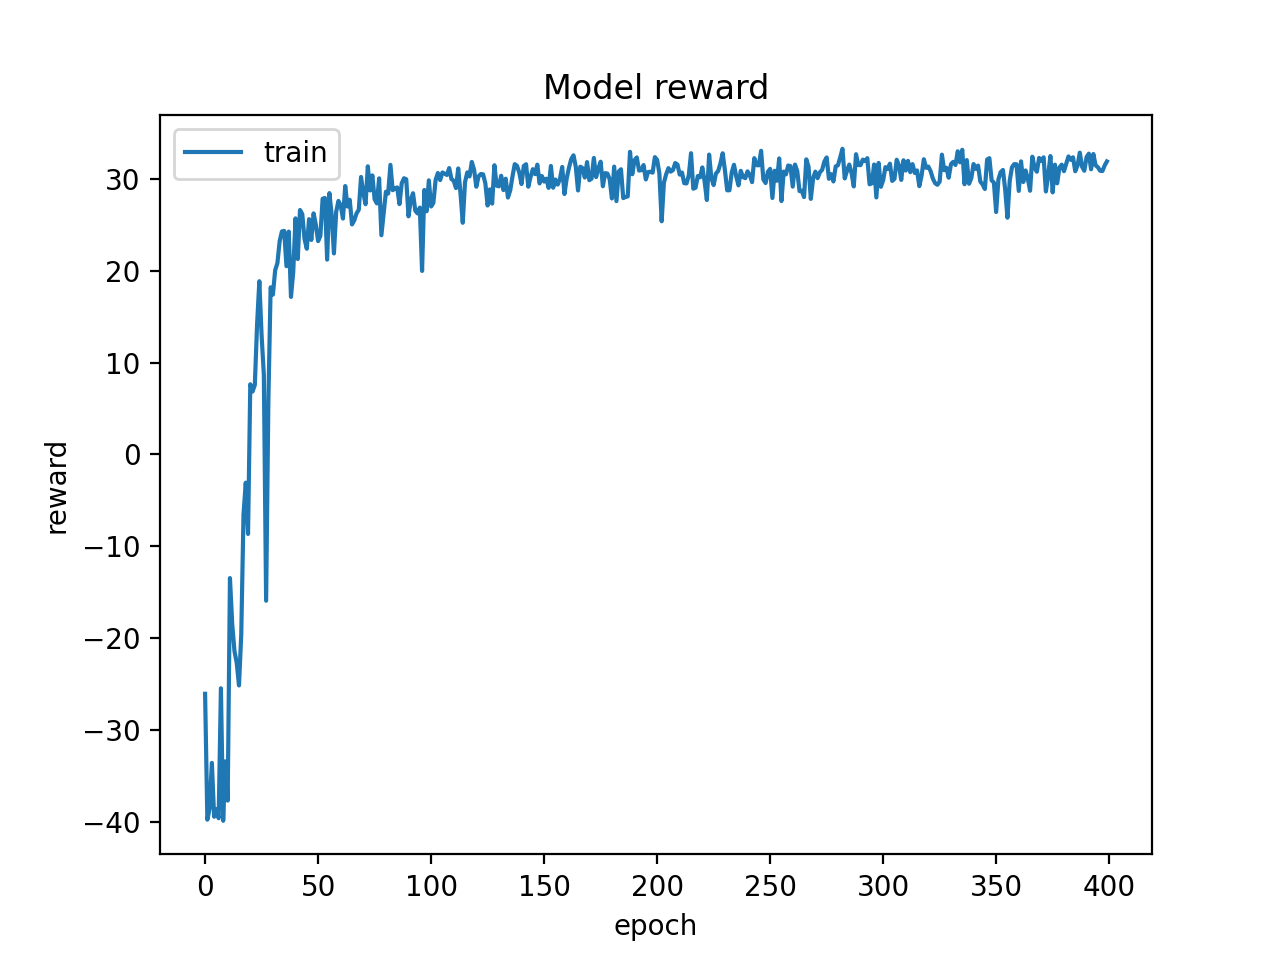
\includegraphics[scale=0.95]{thesis/chatbot/ketqua/img/rewardtrain.png}
    \caption{Biểu đồ đường cong huấn luyện cho phần thưởng}
    \label{fig:rewardtrain}
\end{figure}

\subsubsection{Nhận xét}
Với kết quả biểu diễn ở hình \ref{fig:rewardtrain}, ta thấy:

\begin{itemize}
    \item Giai đoạn đầu, phần thưởng nhận được là cực thấp.
    Vì thời gian đầu, tác nhân cần được khám phá thị trường
    một cách tổng quát nhất.
    \item Tuy nhiên, để phần thưởng nhận được trở nên tích cực,
    nó chỉ mất khoảng 5000 đến 10000 lượt hội thoại.
    \item Độ dốc đường cong ở các epoch cuối là thấp, phần thưởng
    nhận được khá ổn định trong giai đoạn cuối của huấn luyện.
    Chứng tỏ, huấn luyện được mô hình có chính sách (policy) ổn định.
    \item Kết quả cuối huấn luyện của mô hình khá tốt.
    Phần thưởng giao động trên 30 điểm.
\end{itemize}

% Có ba số liệu thống kê của biểu đồ này quan trọng:
% • Độ dốc tiệm cận cho thấy chính sách tốt như thế nào sau khi thuật toán đã ổn định.
% • Mức tối thiểu của đường cong cho thấy phần thưởng phải được hy sinh trước khi nó bắt đầu cải thiện.
% • Việc vượt qua số 0 cho thấy phải mất bao lâu cho đến khi thuật toán thu hồi được chi phí học tập của nó.

Ngoài ra, ta còn có một biểu đồ đường cong huấn luyện biểu diễn
tỉ lệ thành công của hội thoại như hình \ref{fig:successtrain}.
Tỉ lệ thành công được tính của 100 lượt hội thoại.

\begin{figure}[ht!]
    \centering
    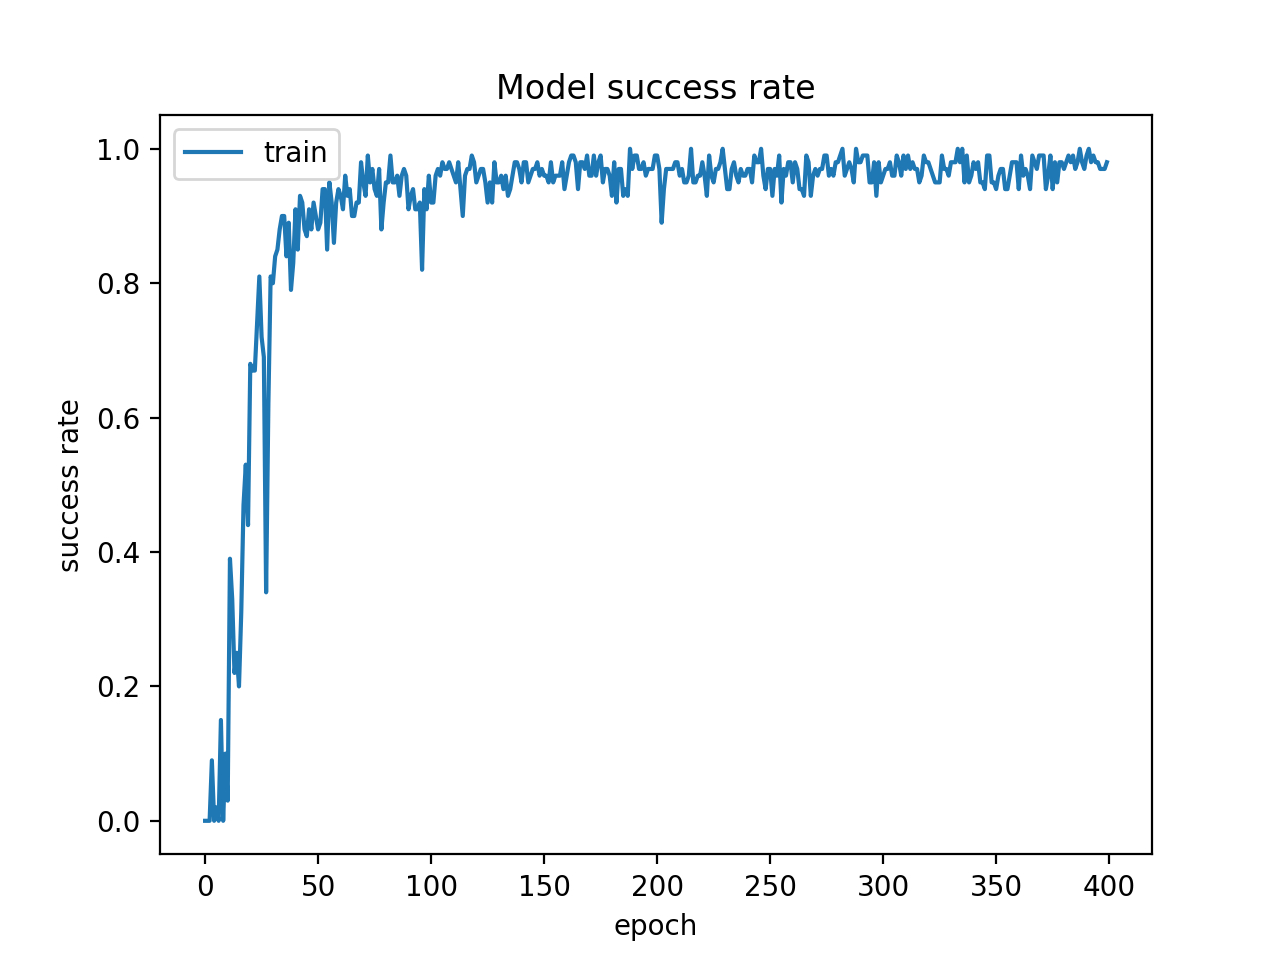
\includegraphics[scale=0.95]{thesis/chatbot/ketqua/img/successtrain.png}
    \caption{Biểu đồ đường cong huấn luyện cho tỉ lệ thành công}
    \label{fig:successtrain}
\end{figure}

\subsubsection{Nhận xét}
Với kết quả biểu diễn ở hình \ref{fig:successtrain}, ta thấy:

\begin{itemize}
    \item Giai đoạn đầu, tỉ lệ thành công là cực thấp. Tương đương
    với phần thưởng nhận được thấp như mô tả ở hình \ref{fig:rewardtrain}.
    \item Tỉ lệ thành công cũng trở nên tốt hơn sau 5000 đến
    10000 lượt hội thoại.
    \item Độ dốc đường cong ở các epoch cuối là thấp, tỉ lệ
    thành công khá ổn định trong giai đoạn cuối của huấn luyện.
    \item Kết quả cuối huấn luyện của mô hình khá tốt.
    Tỉ lệ thành công giao động từ 0.97 đến 1.
\end{itemize}

\subsection{Kiểm thử mô hình sử dụng bộ mô phỏng người dùng}
Như đã trình bày ở mục \ref{sec:usersim}, \textit{User Simulator} là
bộ mô phỏng người dùng thật để tương tác với tác nhân. Sau khi
huấn luyện, ta cũng có thể sử dụng nó để đánh giá mô hình. Việc dùng
bộ mô phỏng người dùng cho việc đánh giá sẽ giảm thiểu thời gian và
công sức rất nhiều so với người dùng thật. Ngoài ra, bằng cách chạy
tự động và với tập dữ liệu mục tiêu người dùng, chúng ta đánh giá
được mô hình với nhiều loại kịch bản khác nhau.

Hệ thống để đánh giá mô hình tương tự như quá trình huấn luyện.
Với bộ mô phỏng người dùng, ta chỉ đánh giá với tiêu chí là cuộc
hội thoại có thành công hay không, cụ thể được mô tả như sau:

\subsubsection{Tiêu chí đánh giá}
Cuộc hội thoại kết thúc thành công khi:

\begin{itemize}
    \item Các thông tin mà tác nhân cung cấp không xung đột với
    các ràng buộc mà người dùng cung cấp.
    \item Hoàn thành đủ mục tiêu của người dùng, các thông tin mà
    người dùng yêu cầu được cung cấp đầy đủ bởi tác nhân.
    \item Tác nhân tìm thấy sản phẩm thỏa mãn mọi yêu cầu của
    người dùng. Mục tiêu cuối cùng của Chatbot này chốt được đơn hàng
    cho người dùng nên trong trường hợp tác nhân tìm thấy thông tin
    sản phẩm nhưng bị từ chối bởi người dùng vẫn tính là không thành công.
\end{itemize}

\subsubsection{Kết quả}
Sử dụng tập mục tiêu người dùng (User Goal) như mô tả ở mục
\ref{subsec:usergoal}, sau 10000 cuộc hội thoại diễn ra, ta đạt được
xác suất \textbf{96\%} cuộc hội thoại thành công.

\subsubsection{Nhận xét}
Với kết quả 96\% cuộc hội thoại thành công, tác nhân đã gần như lúc nào
cũng hoàn thành được nhu cầu của người dùng. Sau khi phân tích cụ thể
các trường hợp không thành công, đa phần đến từ việc tư vấn kích cỡ
sản phẩm phù hợp cho người dùng. Nguyên nhân do dữ liệu về kích cỡ
cơ thể chưa đủ phong phú để tìm được kích cỡ phù hợp, và một phần do
số đo cơ thể người dùng thực sự không phù hợp cho các sản phẩm mà
cửa hàng kinh doanh.

\subsection{Đánh giá từ người dùng thực}
Để nhận đánh giá từ người dùng một cách nhanh chóng và rõ ràng, trong
luận án này, xây dựng một bộ các câu hội thoại/ đoạn hội thoại, gửi
cho một số người dùng thực tế để đánh giá. Ngoài ra, thực hiện so sánh
với một ứng dụng Chatbot tư vấn tương tự khác. Chatbot này không
huấn luyện mô hình mà chỉ thực hiện theo một bộ luật định sẵn (Chatbot
rule-based). Việc này nhằm mục đích so sánh Chatbot huấn luyện theo
mô hình học tăng cường đạt được mục tiêu ứng dụng thực tế nhất định.

\subsubsection{Tiêu chí đánh giá}
Các tiêu chí đánh giá cho các câu thoại bao gồm:

\begin{itemize}
    \item Thỏa mãn yêu cầu người dùng đưa ra
    \item Tính hợp lý, thiết thực của các câu yêu cầu từ tác nhân
    \item Tính tự nhiên, dễ trả lời của các câu yêu cầu từ tác nhân
    \item Tính thiết thực, hữu ích của các thông tin mà tác nhân cung cấp
    \item Tính chính xác của các thông tin mà tác nhân cung cấp
\end{itemize}

Các tiêu chí đánh giá cho toàn bộ hội thoại bao gồm:

\begin{itemize}
    \item Mức độ đáp ứng nhu cầu tư vấn sản phẩm nói chung
    \item Mức độ giao tiếp tự nhiên trong suốt cuộc hội thoại
    \item Đánh giá tổng quan của người dùng
\end{itemize}

Toàn bộ các tiêu chí này sẽ được đánh giá thêm một cột rằng nó có
tốt hơn so với \textit{Chatbot rule-based} hay không.

\subsubsection{Nội dung đánh giá}
Các câu thoại tạo ra để mang đi đánh giá nên thể hiện tất cả các
trường hợp khi người dùng tham dự vào hội thoại. Cụ thể:

Nội dung đánh giá cho các câu thoại thông thường:

\begin{itemize}
    \item Chào hỏi với tác nhân gồm:
    \begin{itemize}
        \item Chào hỏi khi bắt đầu cuộc hội thoại
        \item Chào hỏi ở giữa cuộc hội thoại
        \item Chào hỏi khi kết thúc cuộc hội thoại
        \item Chào hỏi nhiều lần
    \end{itemize}
    \item Cám ơn/tạm biệt với tác nhân gồm:
    \begin{itemize}
        \item Khách hàng cám ơn shop sau khi xác nhận đặt hàng, được
        tư vấn sản phẩm
        \item Khách hàng cám ơn shop sau khi nhận được thông tin
        sản phẩm hữu ích
        \item Khách hàng cám ơn ở những trường hợp không liên quan khác
        \item Cám ơn nhiều lần
    \end{itemize}
    \item Khác: Khách hàng hỏi các thông tin khác không liên quan tới
    tư vấn sản phẩm
\end{itemize}

Tiêu chí đánh giá cho các câu thoại thông thường:

\begin{itemize}
    \item Tính hợp lý: Không hợp lý, phải cải thiện -> Không hợp lý
    lắm, nhưng chấp nhận được -> Hợp lý
    \item Tính tự nhiên: Không tự nhiên, phải cải thiện -> Không
    tự nhiên lắm, nhưng chấp nhận được -> Tự nhiên
    \item Tính hợp lý/ Tính tự nhiên so với \textit{Chatbot rule-based}:
    Tệ hơn -> Như nhau -> Tốt hơn
\end{itemize}

Nội dung đánh giá cho các câu thoại tư vấn:

\begin{itemize}
    \item Yêu cầu cung cấp thông tin sản phẩm. Trường hợp có hàng và
    không có hàng gồm:
    \begin{itemize}
        \item Gửi tên sản phẩm, hỏi đơn giá
        \item Gửi tên sản phẩm, hỏi màu sản phẩm
        \item Gửi tên sản phẩm, hỏi chất liệu sản phẩm
        \item Gửi tên sản phẩm, hỏi kích cỡ sản phẩm
        \item Gửi tên sản phẩm, kích cỡ, hỏi đơn giá
        \item Gửi tên sản phẩm, màu, hỏi đơn giá
        \item Gửi tên sản phẩm, kích cỡ, hỏi màu sản phẩm
        \item Gửi tên sản phẩm, màu, hỏi chất liệu sản phẩm
        \item Gửi tên sản phẩm, kích cỡ, hỏi chất liệu sản phẩm
        \item Gửi tên sản phẩm, màu, hỏi kích cỡ sản phẩm
        \item Gửi tên sản phẩm, hỏi còn hàng hay không
        \item Gửi tên sản phẩm, màu, hỏi còn hàng hay không
        \item Gửi tên sản phẩm, kích cỡ, hỏi còn hàng hay không
        \item Gửi tên sản phẩm, màu, kích cỡ, hỏi còn hàng hay không
    \end{itemize}
    \item Tư vấn chọn kích cỡ:
    \begin{itemize}
        \item Chỉ gửi chiều cao
        \item Chỉ nhập cân nặng
        \item Chỉ gửi vòng eo
        \item Gửi chiều cao, cân nặng
        \item Gửi chiều cao, vòng eo
        \item Gửi vòng eo, cân nặng
        \item Gửi chiều cao, cân nặng, vòng eo. Trường hợp có
        kích cỡ phù hợp
        \item Gửi chiều cao, cân nặng, vòng eo. Trường hợp không có
        kích cỡ phù hợp
    \end{itemize}
    \item Đặt hàng:
    \begin{itemize}
        \item Chỉ gửi tên sản phẩm
        \item Chỉ gửi màu sản phẩm
        \item Chỉ gửi kích cỡ sản phẩm
        \item Chỉ gửi số lượng sản phẩm
        \item Gửi màu, số lượng sản phẩm
        \item Gửi màu, kích cỡ sản phẩm
        \item Gửi kích cỡ, số lượng sản phẩm
        \item Gửi tên sản phẩm, màu
        \item Gửi tên sản phẩm, kích cỡ
        \item Gửi tên sản phẩm, số lượng
        \item Gửi tên sản phẩm, màu, kích cỡ
        \item Gửi tên sản phẩm, màu, số lượng
        \item Gửi tên sản phẩm, kích cỡ, số lượng
        \item Gửi tên sản phẩm, màu, kích cỡ, số lượng
    \end{itemize}
\end{itemize}

Tiêu chí đánh giá cho các câu thoại tư vấn:

\begin{itemize}
    \item Thỏa mãn yêu cầu người dùng đưa ra: Không thỏa mãn ->
    Chấp nhận được -> Thỏa mãn
    \item Tính hợp lý, thiết thực: Không hợp lý, phải cải thiện ->
    Không hợp lý lắm, nhưng chấp nhận được -> Hợp lý
    \item Tính tự nhiên, dễ trả lời: Không tự nhiên, phải cải thiện
    -> Không tự nhiên lắm, nhưng chấp nhận được -> Tự nhiên
    \item Tính thiết thực, hữu ích: Không thiết thực -> Chấp nhận
    được -> Thiết thực
    \item Tính chính xác: Không chính xác -> Chấp nhận được ->
    Chính xác
    \item So sánh với \textit{Chatbot rule-based} các tiêu chí trên:
    Tệ hơn -> Như nhau -> Tốt hơn
\end{itemize}

Nội dung đánh giá cho các hội thoại:

\begin{itemize}
    \item Hội thoại hỏi các thông tin của sản phẩm và chốt đơn hàng
    \item Hội thoại hỏi sản phẩm, mà cửa hàng không bán hoặc đã hết
    \item Hội thoại hỏi các thông tin của sản phẩm. Trường hợp các
    thông tin không tìm thấy sản phẩm phù hợp
    \item Tư vấn kích cỡ sản phẩm phù hợp với khách hàng
    \item Tư vấn kích cỡ sản phẩm phù hợp với khách hàng. Trường hợp
    không có kích cỡ thích hợp
    \item Thay đổi sản phẩm sau khi đặt hàng
\end{itemize}

Tiêu chí đánh giá cho các hội thoại:

\begin{itemize}
    \item Mức độ đáp ứng nhu cầu tư vấn sản phẩm nói chung: đánh giá
    5 mức độ từ chưa đáp ứng đến rất đầy đủ
    \item Mức độ giao tiếp tự nhiên: đánh giá 5 mức độ từ không
    tự nhiên đến rất tự nhiên
    \item Đánh giá tổng quan: với mức điểm từ một sao đến 5 sao
    \item So sánh với \textit{Chatbot rule-based} các tiêu chí trên:
    Tệ hơn -> Như nhau -> Tốt hơn
\end{itemize}

\subsubsection{Kết quả đánh giá}

\subsubsection{Tiêu chí thỏa mãn yêu cầu người dùng đưa ra}
Hình \ref{fig:tieuchi1} mô tả kết quả đánh giá của người dùng cho
tiêu chí thỏa mãn yêu cầu người dùng đưa ra khi Chatbot trả về kết quả.

\begin{figure}[ht!]
    \centering
    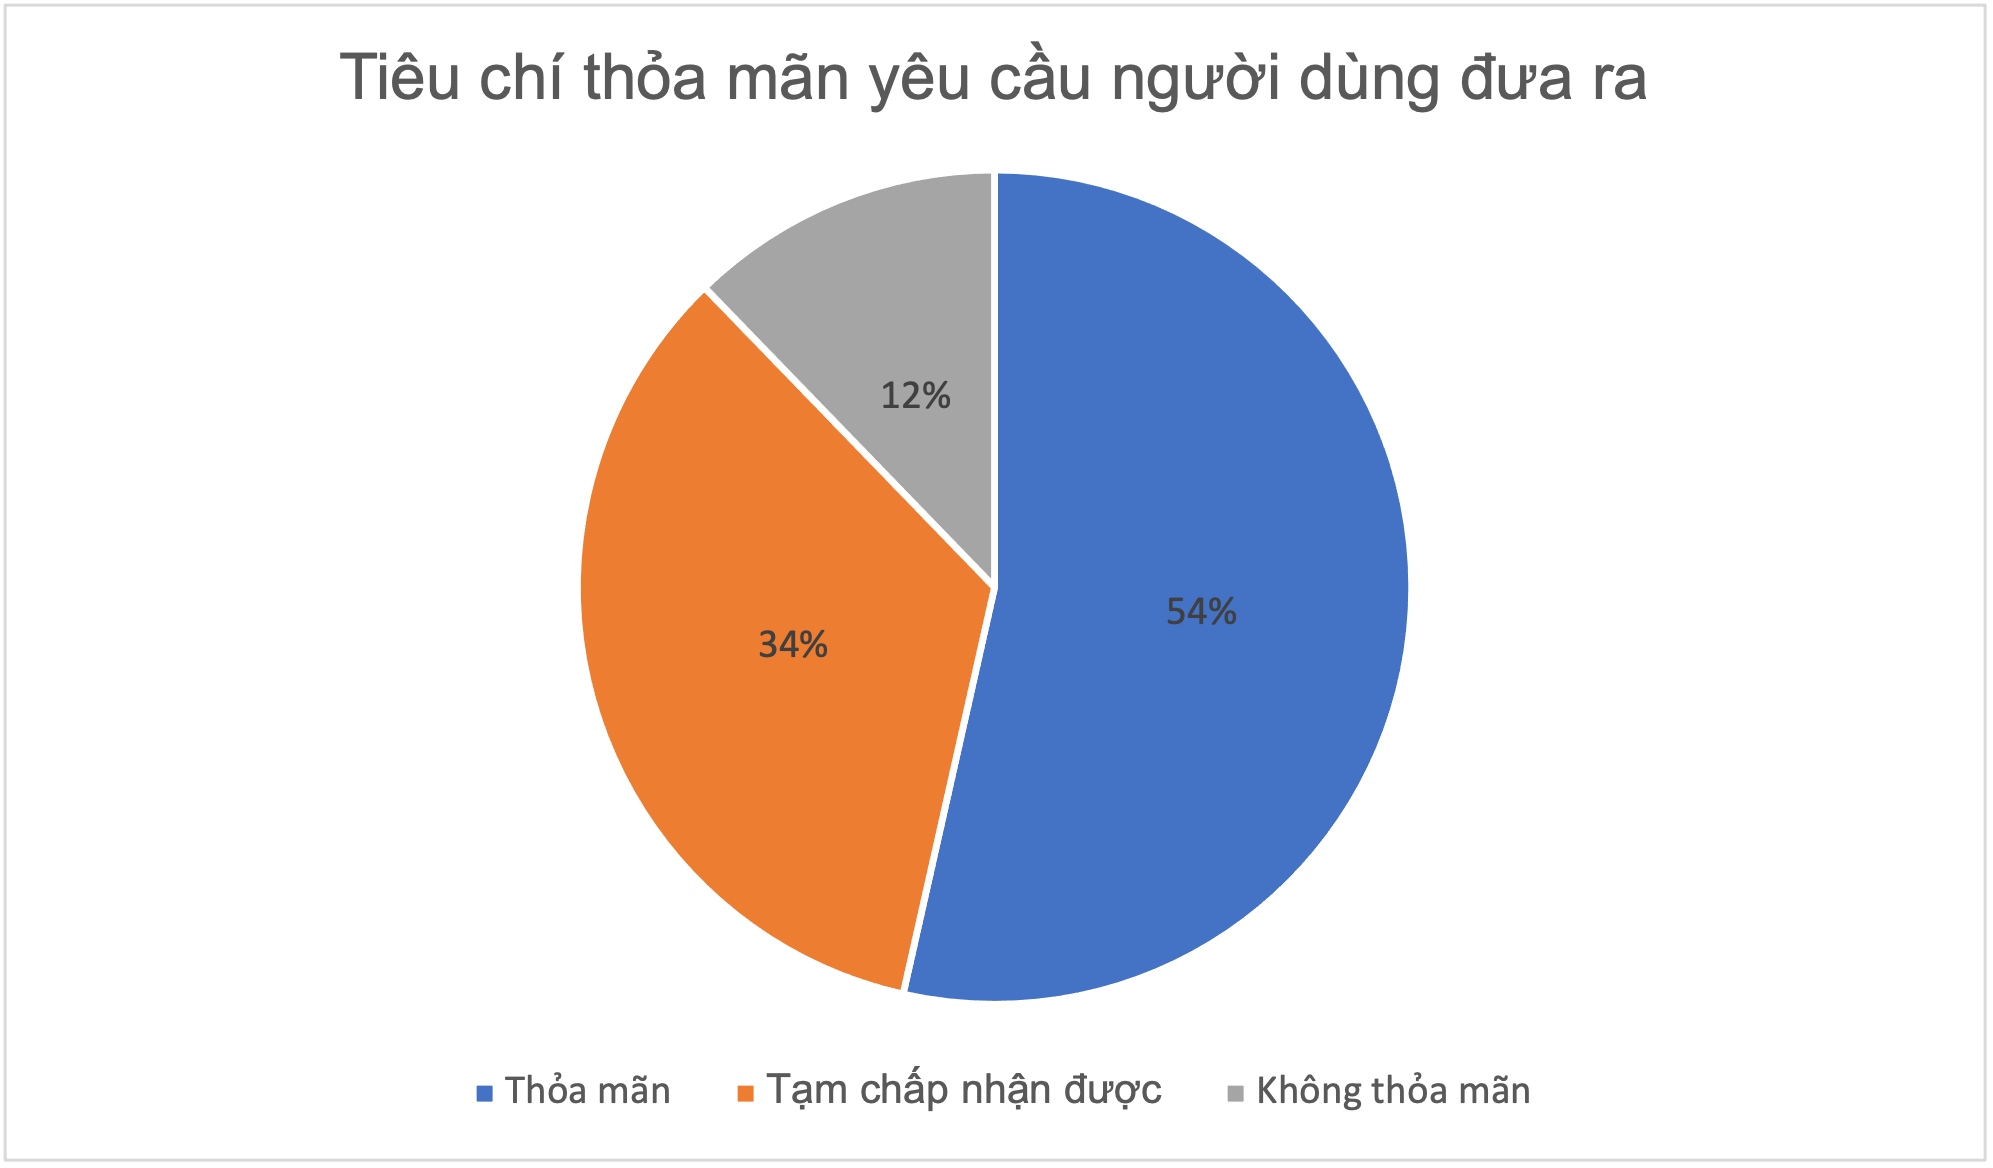
\includegraphics[scale=0.91]{thesis/chatbot/ketqua/img/tieuchi1.png}
    \caption{Kết quả đánh giá tiêu chí thỏa mãn yêu cầu người dùng}
    \label{fig:tieuchi1}
\end{figure}

\textbf{Nhận xét:}
Có 88\% nhận xét từ tạm chấp nhận được cho đến thỏa mãn hết các
yêu cầu. Trong đó hơn 50\% là thỏa mãn. Chỉ có 12\% nhận xét là không
thỏa mãn. Sau khi phân tích cụ thể các kết quả đánh giá không
thỏa mãn, nhận thấy các đánh giá này đa phần đến từ khi người dùng
yêu cầu một thông tin nào đó của sản phẩm không tồn tại trong cơ sở
dữ liệu (cửa hàng không bán hoặc hết hàng) và không cung cấp được
thông tin họ yêu cầu.

\subsubsection{So sánh với Chatbot rule-based}
Hình \ref{fig:tieuchi12} mô tả kết quả đánh giá của người dùng khi
so sánh tiêu chí thỏa mãn yêu cầu người dùng đưa ra với Chatbot
rule-based.

\begin{figure}[ht!]
    \centering
    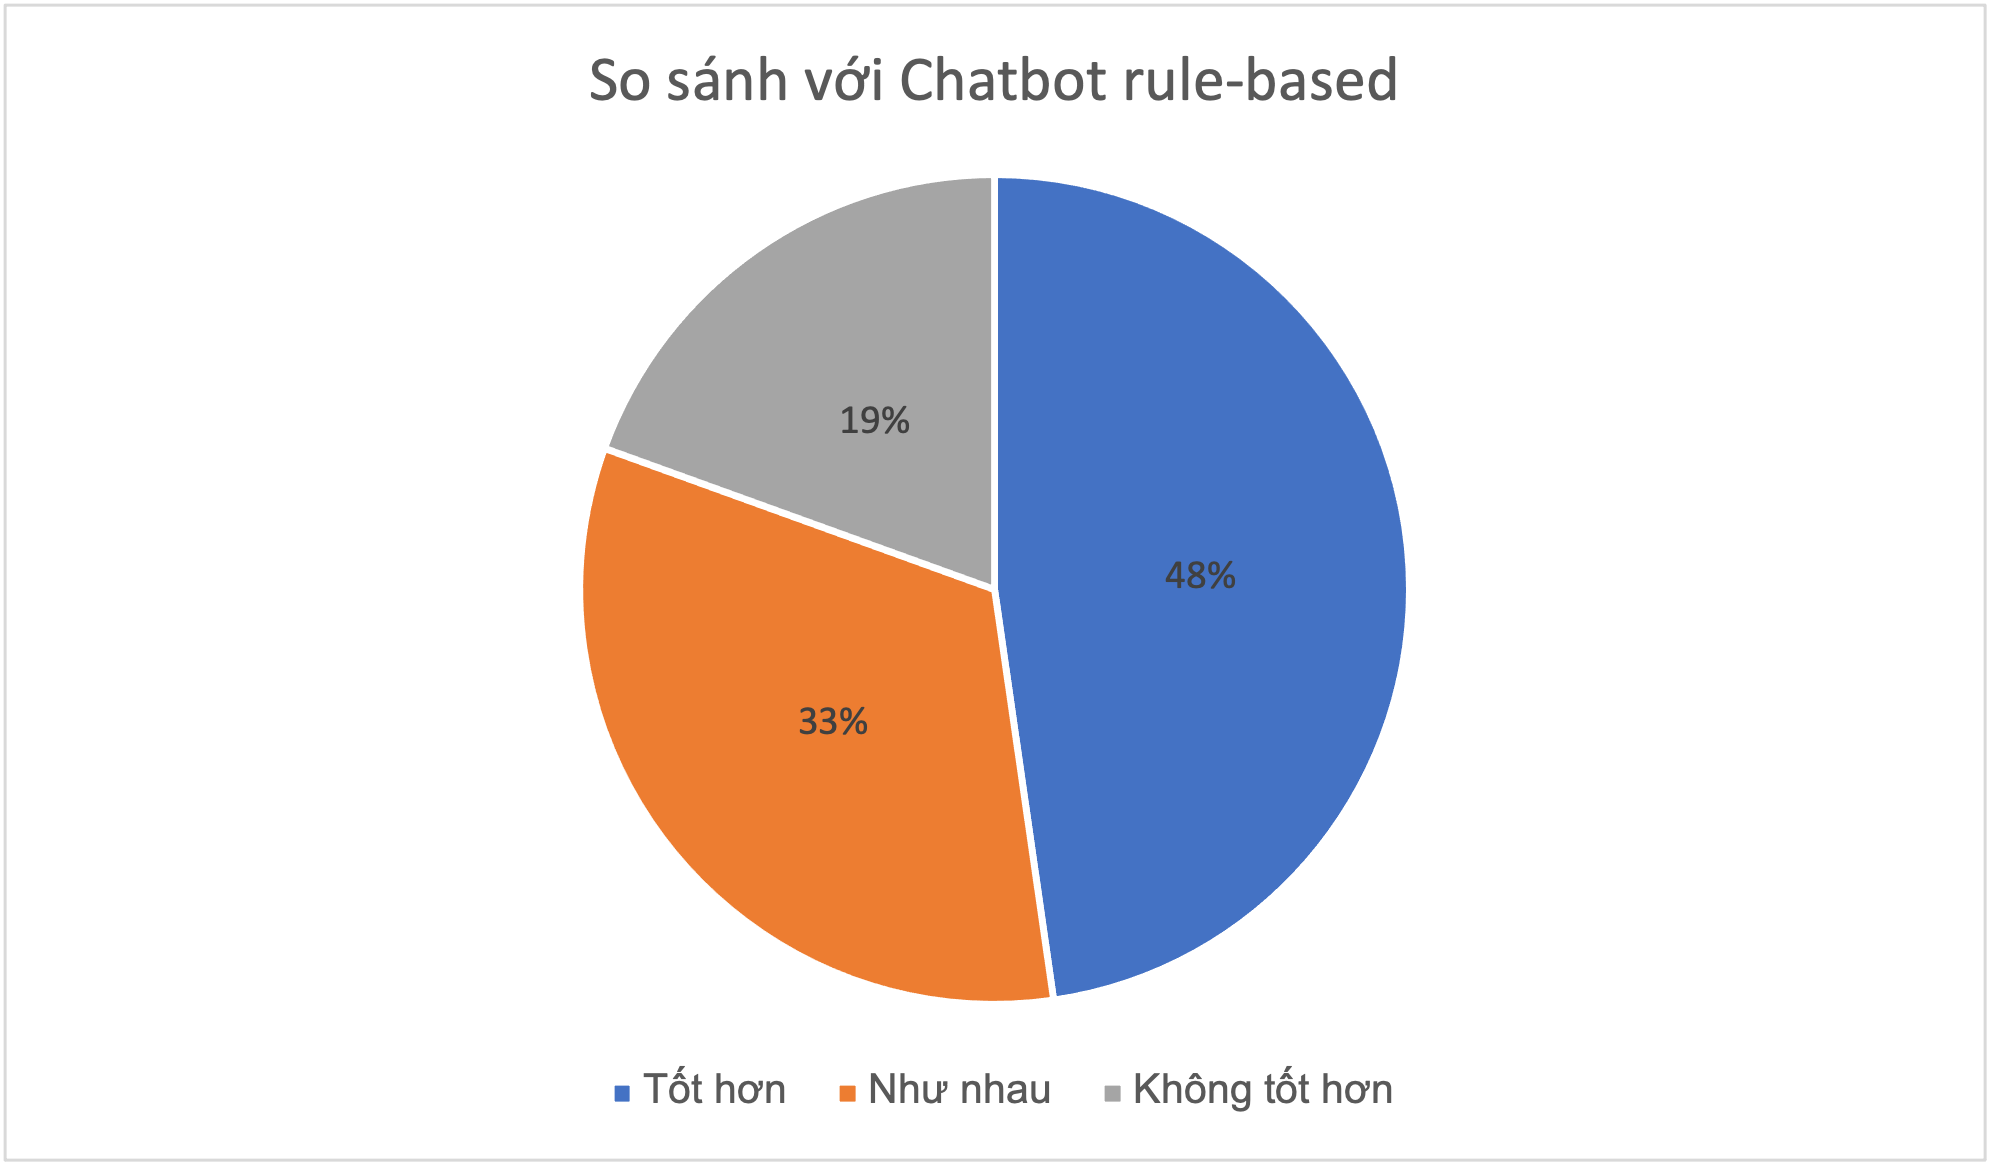
\includegraphics[scale=0.91]{thesis/chatbot/ketqua/img/tieuchi1_2.png}
    \caption{Kết quả so sánh với Chatbot rule-based}
    \label{fig:tieuchi12}
\end{figure}

\textbf{Nhận xét:}
Có hơn 80\% đánh giá là tốt hơn hoặc tương đương với Chatbot
rule-based. Có 19\% là không tốt hơn. Sau khi phân tích cụ thể các
kết quả đánh giá không tốt, nhận thấy Chatbot rule-based này sẽ
liệt kê tất cả thông tin của sản phẩm trong lượt đầu. Việc này
thỏa mãn một số người dùng tốt hơn Chatbot khi sử dụng học tăng cường.

\subsubsection{Tiêu chí về tính hợp lý, thiết thực của các câu
yêu cầu từ tác nhân}
Hình \ref{fig:tieuchi2} mô tả kết quả đánh giá của người dùng cho
tiêu chí tính hợp lý, thiết thực của các câu yêu cầu từ tác nhân.

\begin{figure}[ht!]
    \centering
    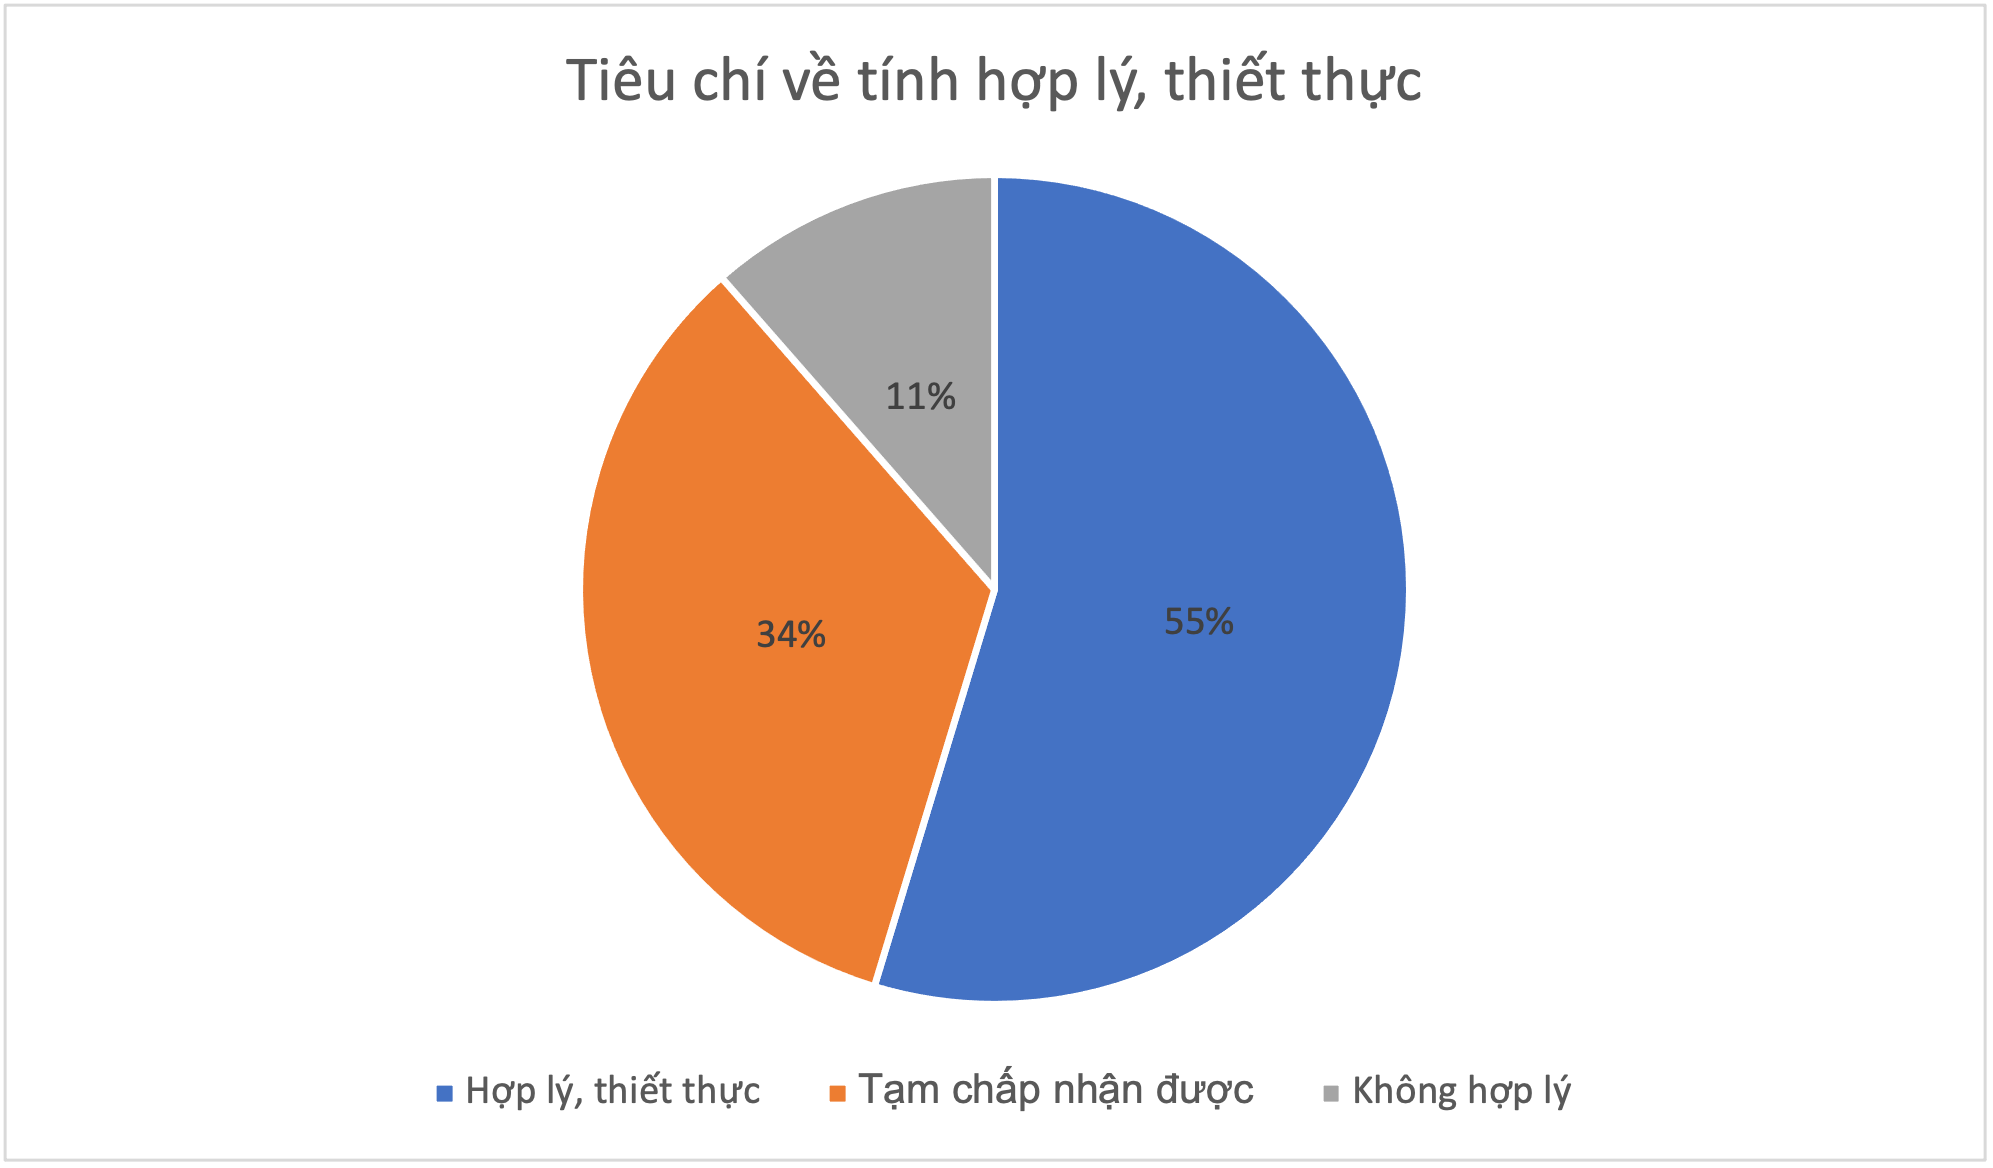
\includegraphics[scale=0.91]{thesis/chatbot/ketqua/img/tieuchi2.png}
    \caption{Kết quả đánh giá tiêu chí tính hợp lý, thiết thực}
    \label{fig:tieuchi2}
\end{figure}

\textbf{Nhận xét:}
Có gần 90\% nhận xét từ tạm chấp nhận được cho đến hợp lý. Trong đó
hơn 50\% là hợp lý. Chỉ có 11\% nhận xét là không hợp lý. Sau khi
phân tích cụ thể các kết quả đánh giá không hợp lý, nhận thấy các
đánh giá này đa phần đến từ khi người dùng yêu cầu một thông tin
nào đó của sản phẩm, họ mong muốn Chatbot mau chóng trả lời thông tin
mà họ cần thay vì phải trải qua một số các câu thoại yêu cầu khác
trước khi trả về kết quả.

\subsubsection{So sánh với Chatbot rule-based}
Hình \ref{fig:tieuchi22} mô tả kết quả đánh giá của người dùng khi
so sánh tiêu chí tính hợp lý, thiết thực với Chatbot rule-based.

\begin{figure}[ht!]
    \centering
    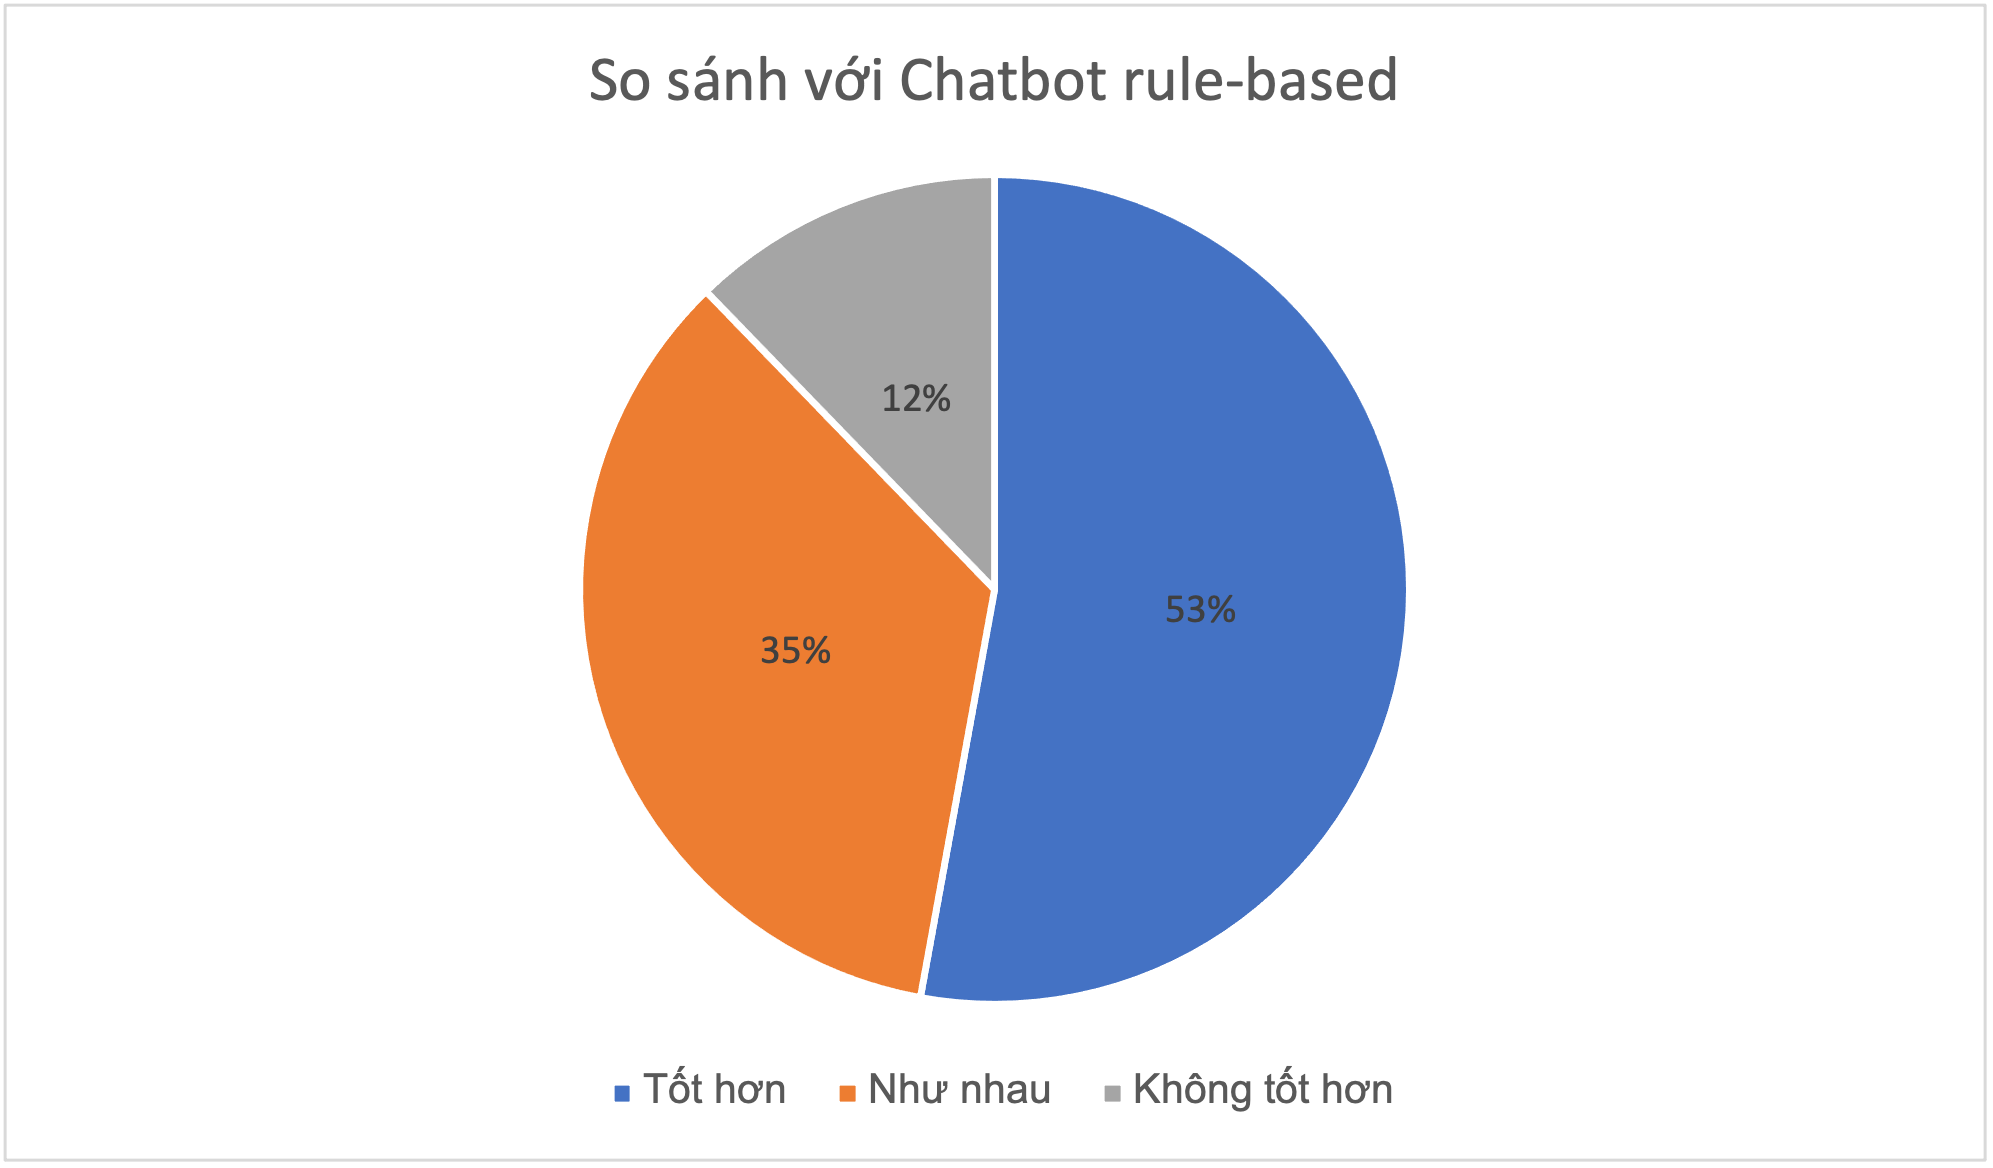
\includegraphics[scale=0.91]{thesis/chatbot/ketqua/img/tieuchi2_2.png}
    \caption{Kết quả so sánh với Chatbot rule-based}
    \label{fig:tieuchi22}
\end{figure}

\textbf{Nhận xét:}
Có gần 90\% đánh giá là tốt hơn hoặc tương đương với Chatbot
rule-based. Có 12\% là không tốt hơn. Sau khi phân tích cụ thể các
kết quả đánh giá không tốt, nhận thấy tương tự với lí do trên,
Chatbot rule-based này sẽ liệt kê tất cả thông tin của sản phẩm
trong lượt đầu. Việc này thỏa mãn một số người dùng tốt hơn Chatbot
khi sử dụng học tăng cường.

\subsubsection{Tiêu chí về tính tự nhiên, dễ trả lời của các câu
yêu cầu từ tác nhân}
Hình \ref{fig:tieuchi3} mô tả kết quả đánh giá của người dùng cho
tiêu chí tính tự nhiên, dễ trả lời của các câu yêu cầu từ tác nhân.

\begin{figure}[ht!]
    \centering
    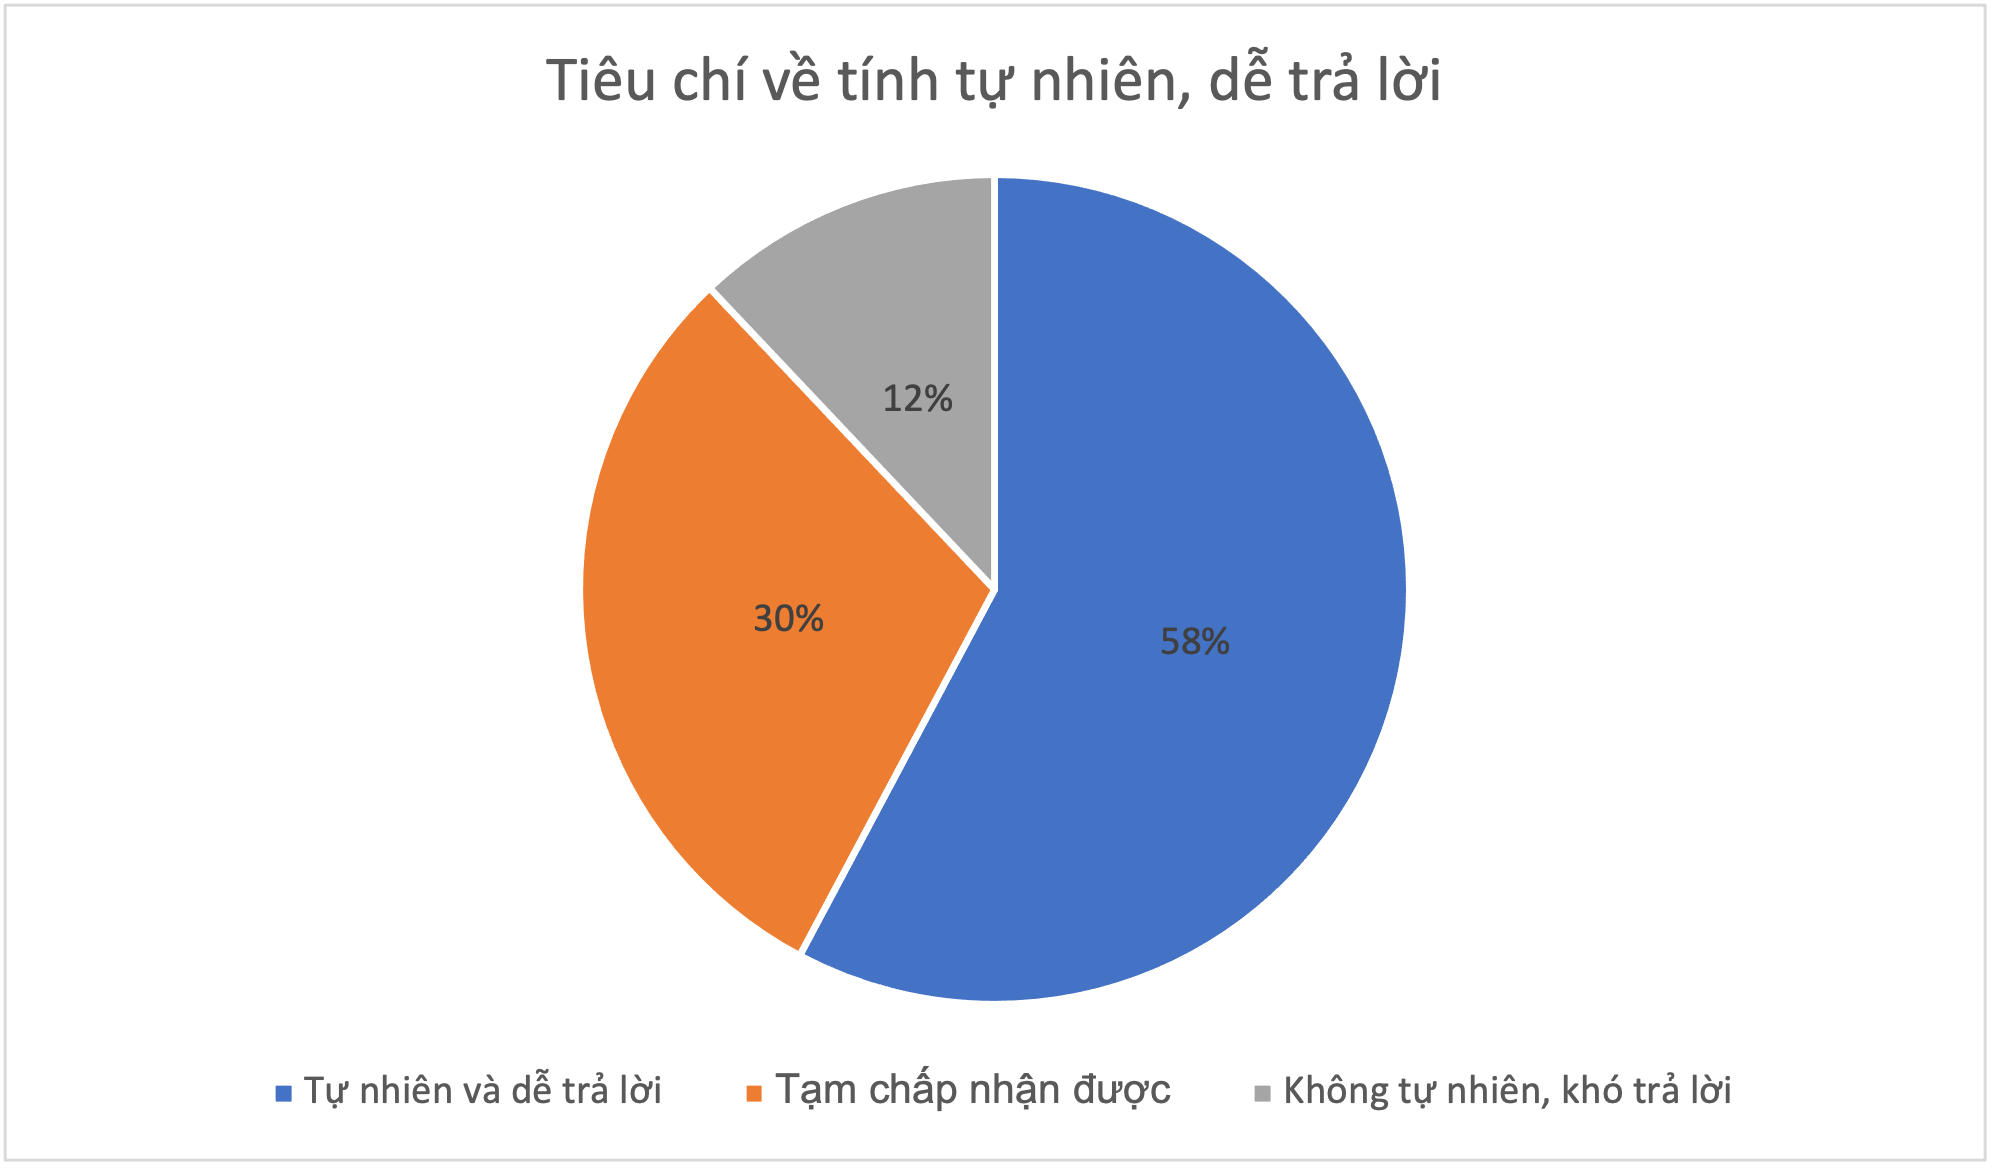
\includegraphics[scale=0.91]{thesis/chatbot/ketqua/img/tieuchi3.png}
    \caption{Kết quả đánh giá tiêu chí tính tự nhiên, dễ trả lời}
    \label{fig:tieuchi3}
\end{figure}

\textbf{Nhận xét:}
Có gần 90\% nhận xét từ tạm chấp nhận được cho đến tự nhiên. Trong đó
hơn 50\% là tự nhiên. Chỉ có 12\% nhận xét là không tự nhiên. Sau khi
phân tích cụ thể các kết quả đánh giá không tự nhiên, nhận thấy các
đánh giá này có thể đến từ bộ sinh phản hồi chưa phù hợp, dẫn tới các
câu gây khó hiểu hoặc hiểu nhầm.

\subsubsection{So sánh với Chatbot rule-based}
Hình \ref{fig:tieuchi32} mô tả kết quả đánh giá của người dùng khi
so sánh tiêu chí tính tự nhiên, dễ trả lời với Chatbot rule-based.

\begin{figure}[ht!]
    \centering
    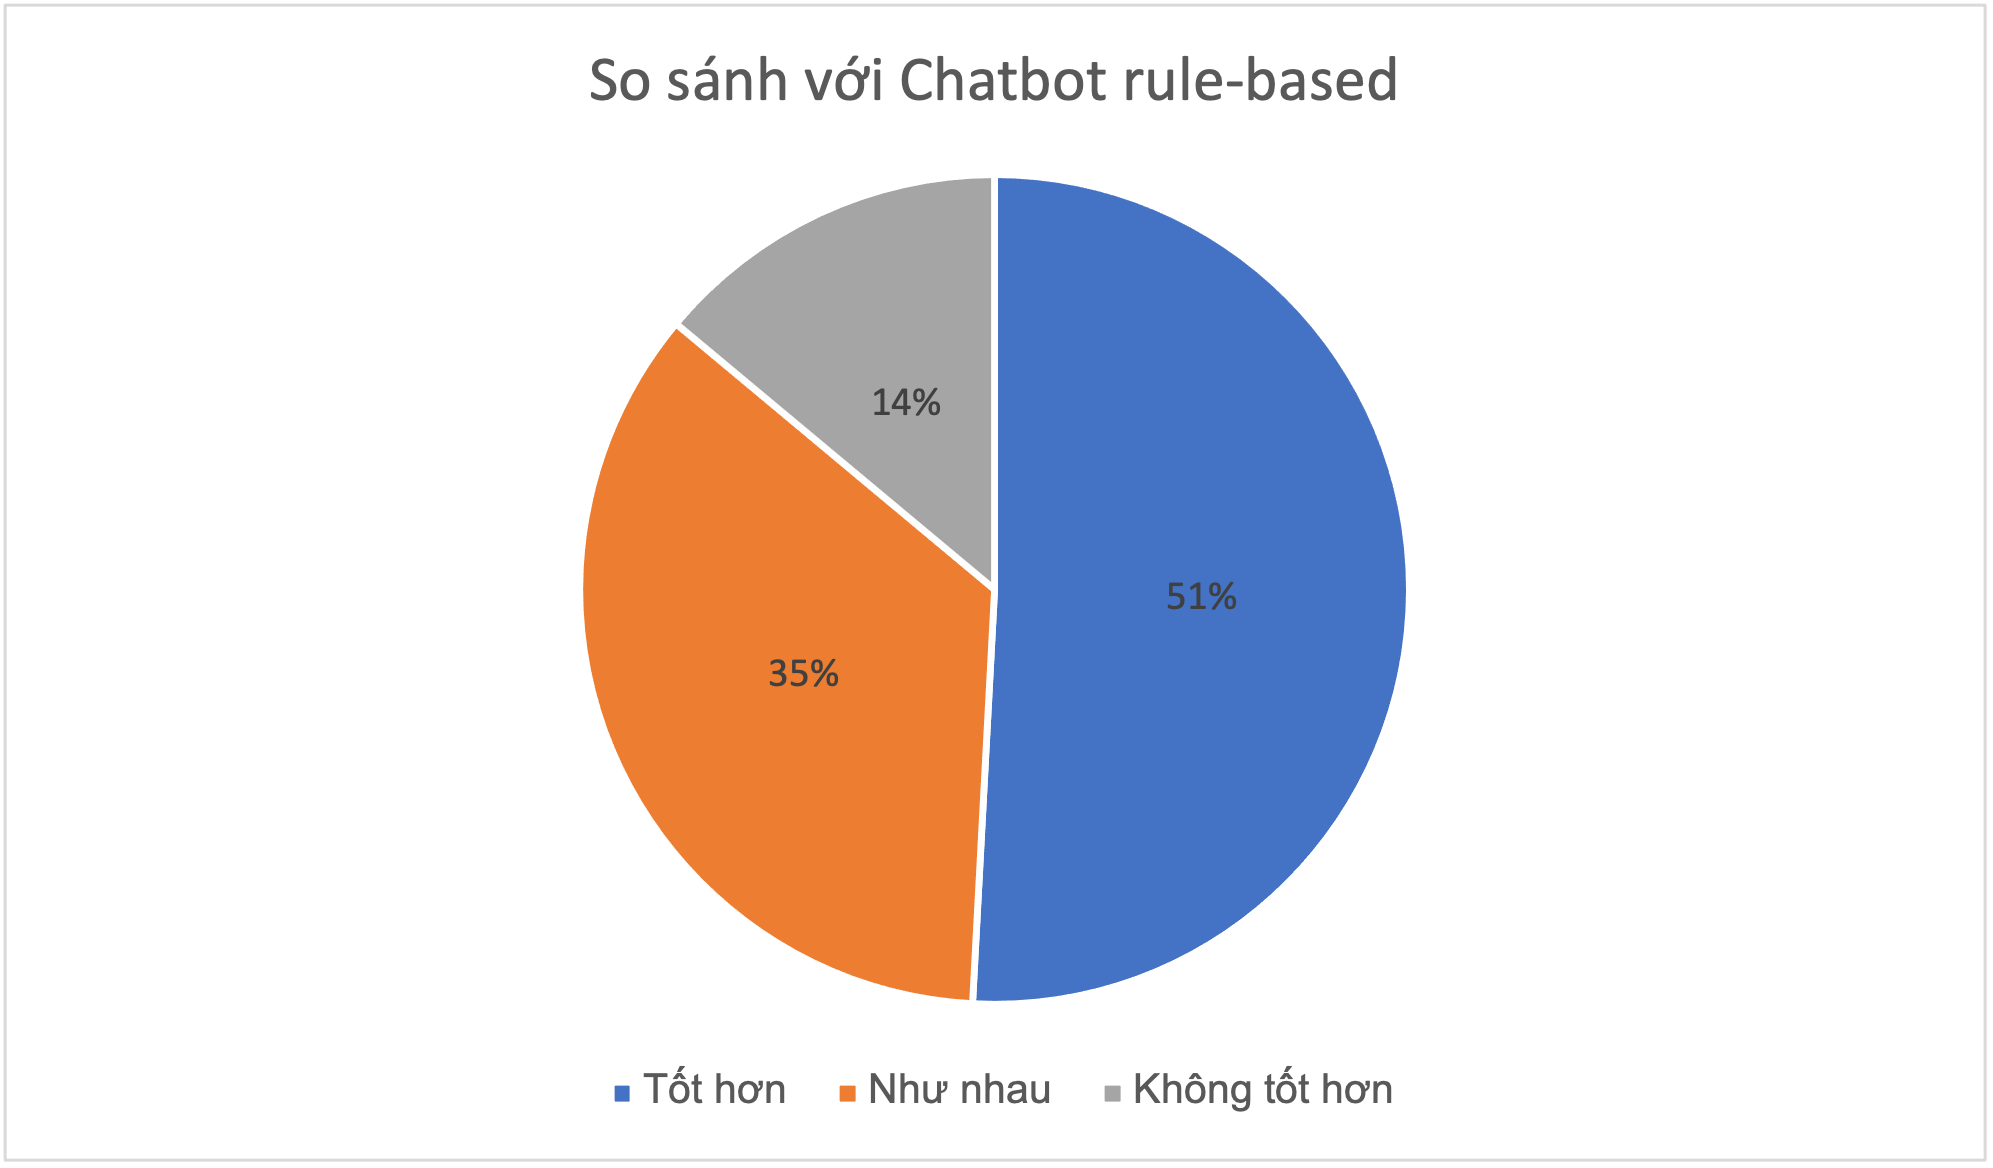
\includegraphics[scale=0.91]{thesis/chatbot/ketqua/img/tieuchi3_2.png}
    \caption{Kết quả so sánh với Chatbot rule-based}
    \label{fig:tieuchi32}
\end{figure}

\textbf{Nhận xét:}
Có gần 90\% đánh giá là tốt hơn hoặc tương đương với Chatbot rule-based.
Có 14\% là không tốt hơn. Sau khi phân tích cụ thể các kết quả đánh giá
không tốt, nhận thấy tương tự với lí do trên, Chatbot rule-based này sinh
câu phản hồi mà thỏa mãn một số người dùng tốt hơn Chatbot được
xây dựng trong đề tài.

\subsubsection{Tiêu chí về tính thiết thực, hữu ích của các thông tin
mà tác nhân cung cấp}
Hình \ref{fig:tieuchi4} mô tả kết quả đánh giá của người dùng cho tiêu chí
tính thiết thực, hữu ích của các thông tin mà tác nhân cung cấp.

\begin{figure}[ht!]
    \centering
    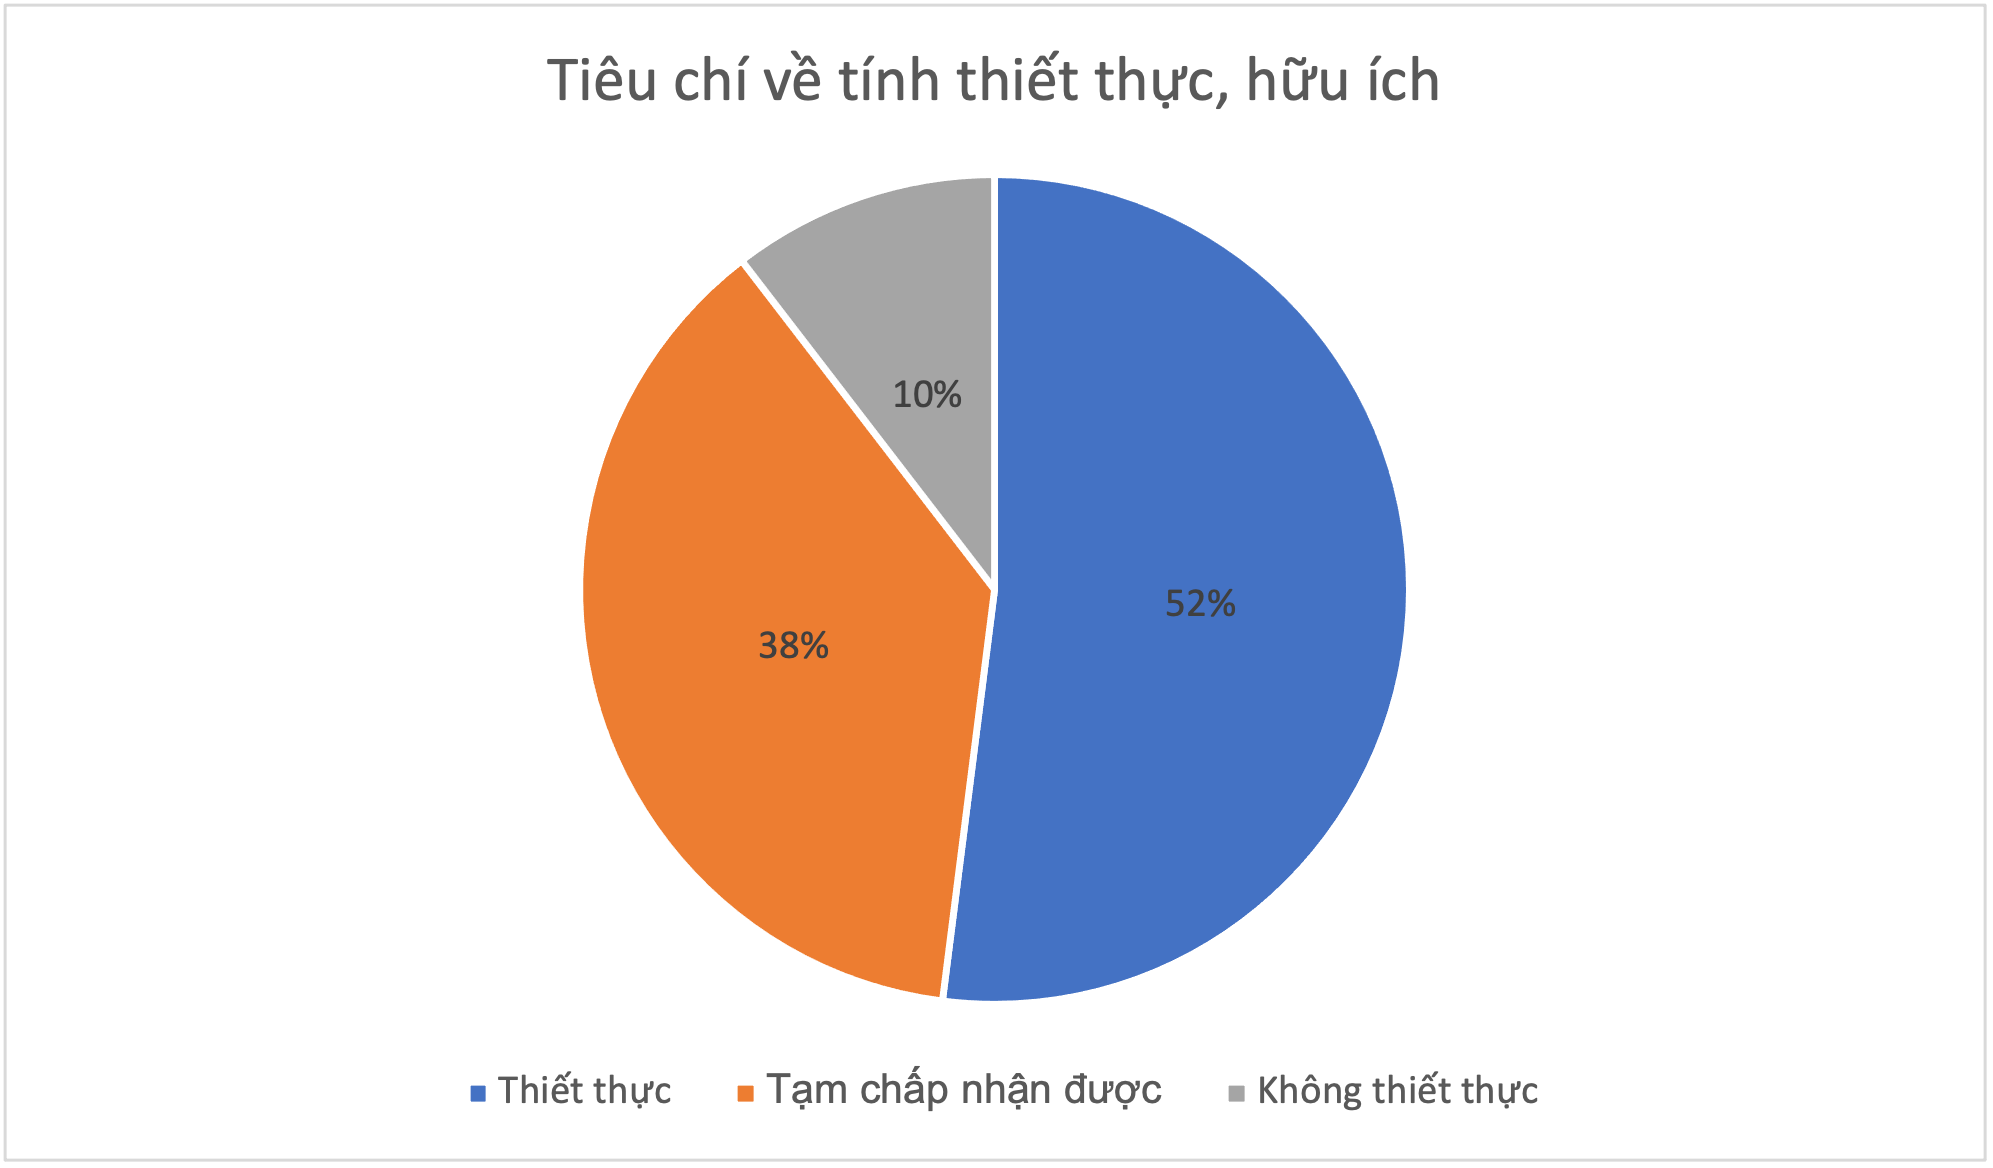
\includegraphics[scale=0.91]{thesis/chatbot/ketqua/img/tieuchi4.png}
    \caption{Kết quả đánh giá tiêu chí tính thiết thực, hữu ích}
    \label{fig:tieuchi4}
\end{figure}

\begin{figure}[ht!]
    \centering
    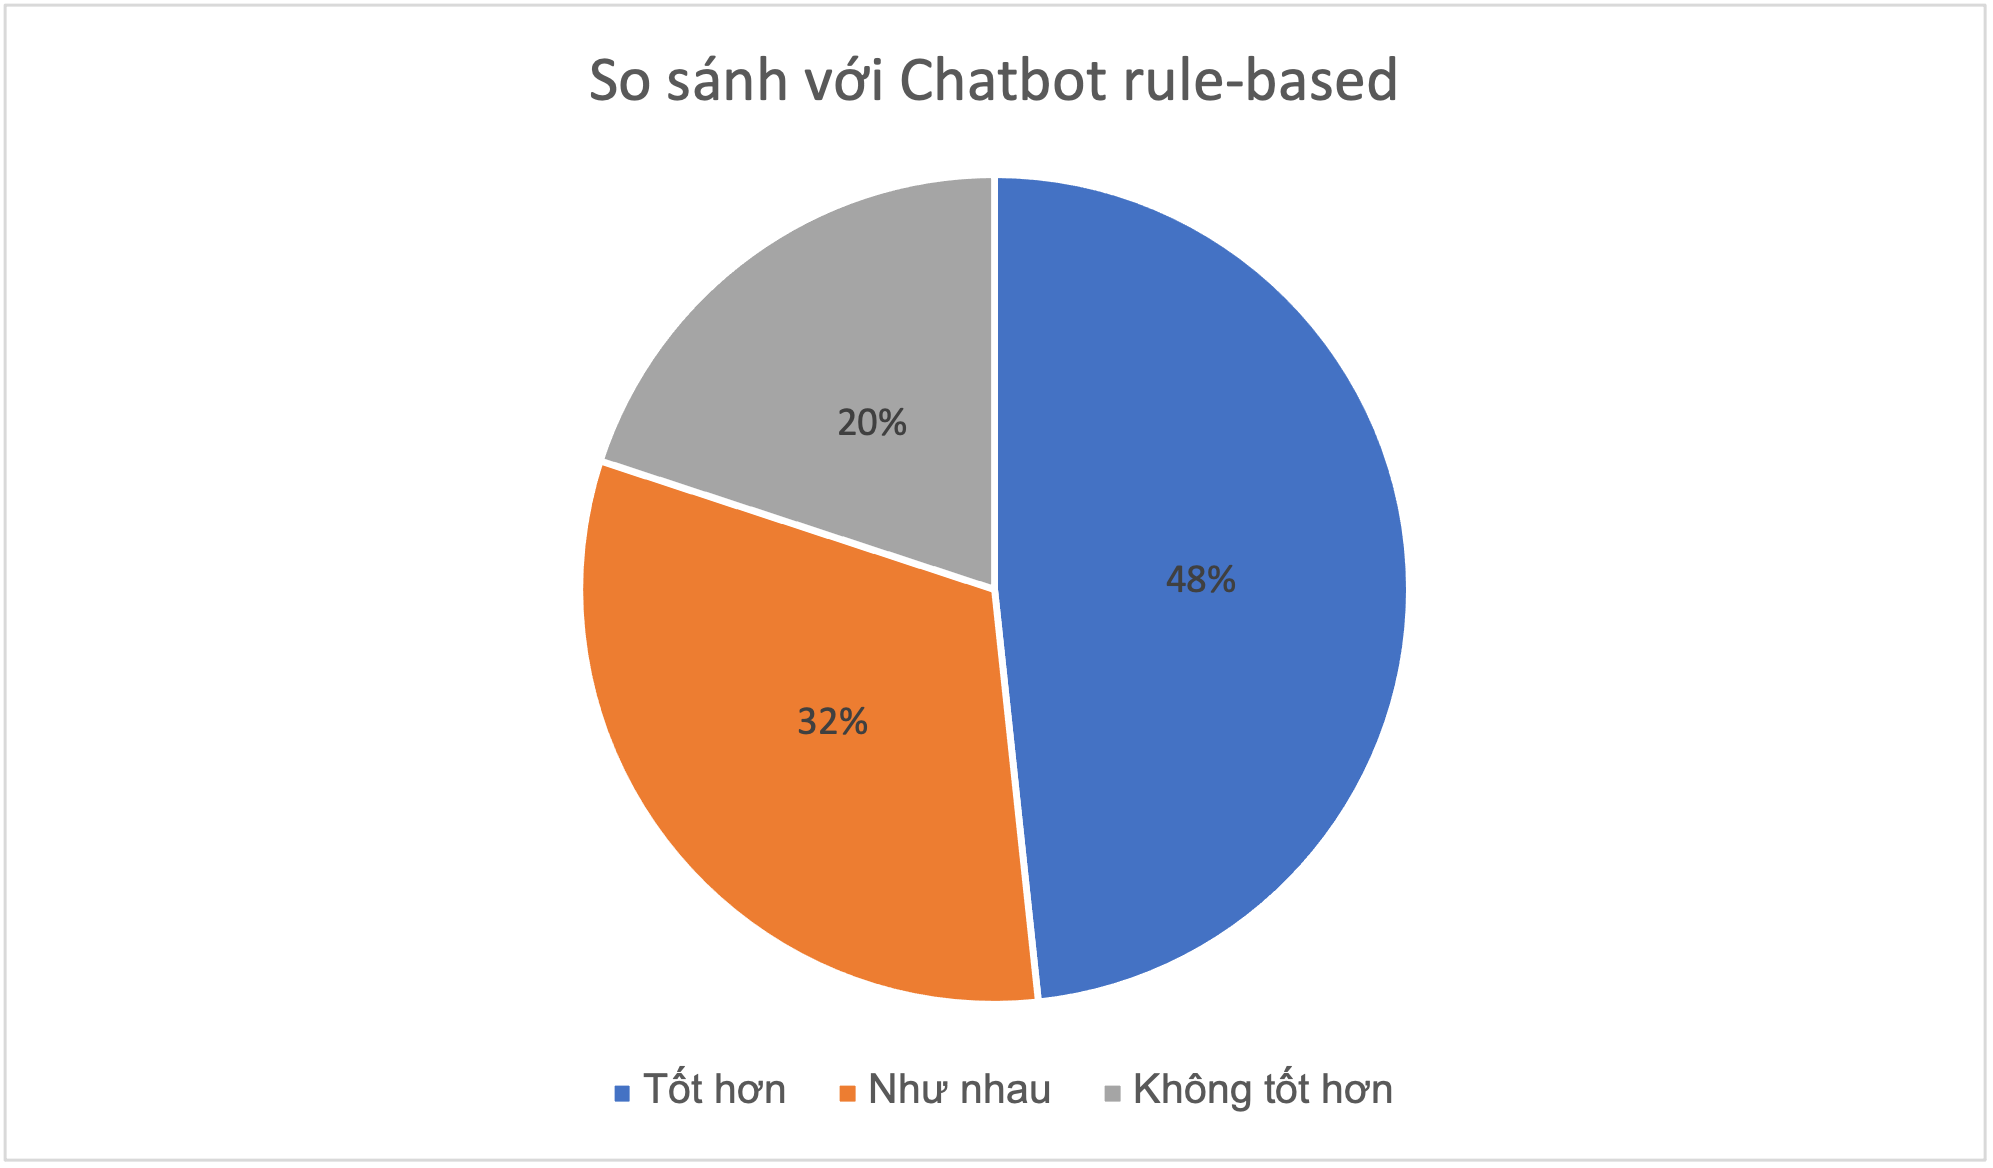
\includegraphics[scale=0.91]{thesis/chatbot/ketqua/img/tieuchi4_2.png}
    \caption{Kết quả so sánh với Chatbot rule-based}
    \label{fig:tieuchi42}
\end{figure}

\textbf{Nhận xét:}
Có 90\% nhận xét từ tạm chấp nhận được cho đến thiết thực. Trong đó
hơn 50\% là thiết thực. Chỉ có 10\% nhận xét là không thiết thực.
Nhận thấy việc gợi ý, cung cấp thông tin về sản phẩm giúp Chatbot
có thể thể hiện được khả năng hiểu vấn đề và khả năng cung cấp
thông tin có ích cho người dùng.

\subsubsection{So sánh với Chatbot rule-based}
Hình \ref{fig:tieuchi42} mô tả kết quả đánh giá của người dùng khi
so sánh tiêu chí tính thiết thực, hữu ích với Chatbot rule-based.

\textbf{Nhận xét:}
Có 80\% đánh giá là tốt hơn hoặc tương đương với Chatbot rule-based.
Có 20\% là không tốt hơn. Sau khi phân tích cụ thể các kết quả
đánh giá không tốt, nhận thấy Chatbot rule-based này sẽ liệt kê tất cả
thông tin của sản phẩm trong lượt đầu. Việc này thỏa mãn một số
người dùng tốt hơn Chatbot khi sử dụng học tăng cường.

\subsubsection{Tiêu chí về tính chính xác của các thông tin mà
tác nhân cung cấp}
Hình \ref{fig:tieuchi5} mô tả kết quả đánh giá của người dùng cho
tiêu chí tính chính xác của các thông tin mà tác nhân cung cấp.

\begin{figure}[ht!]
    \centering
    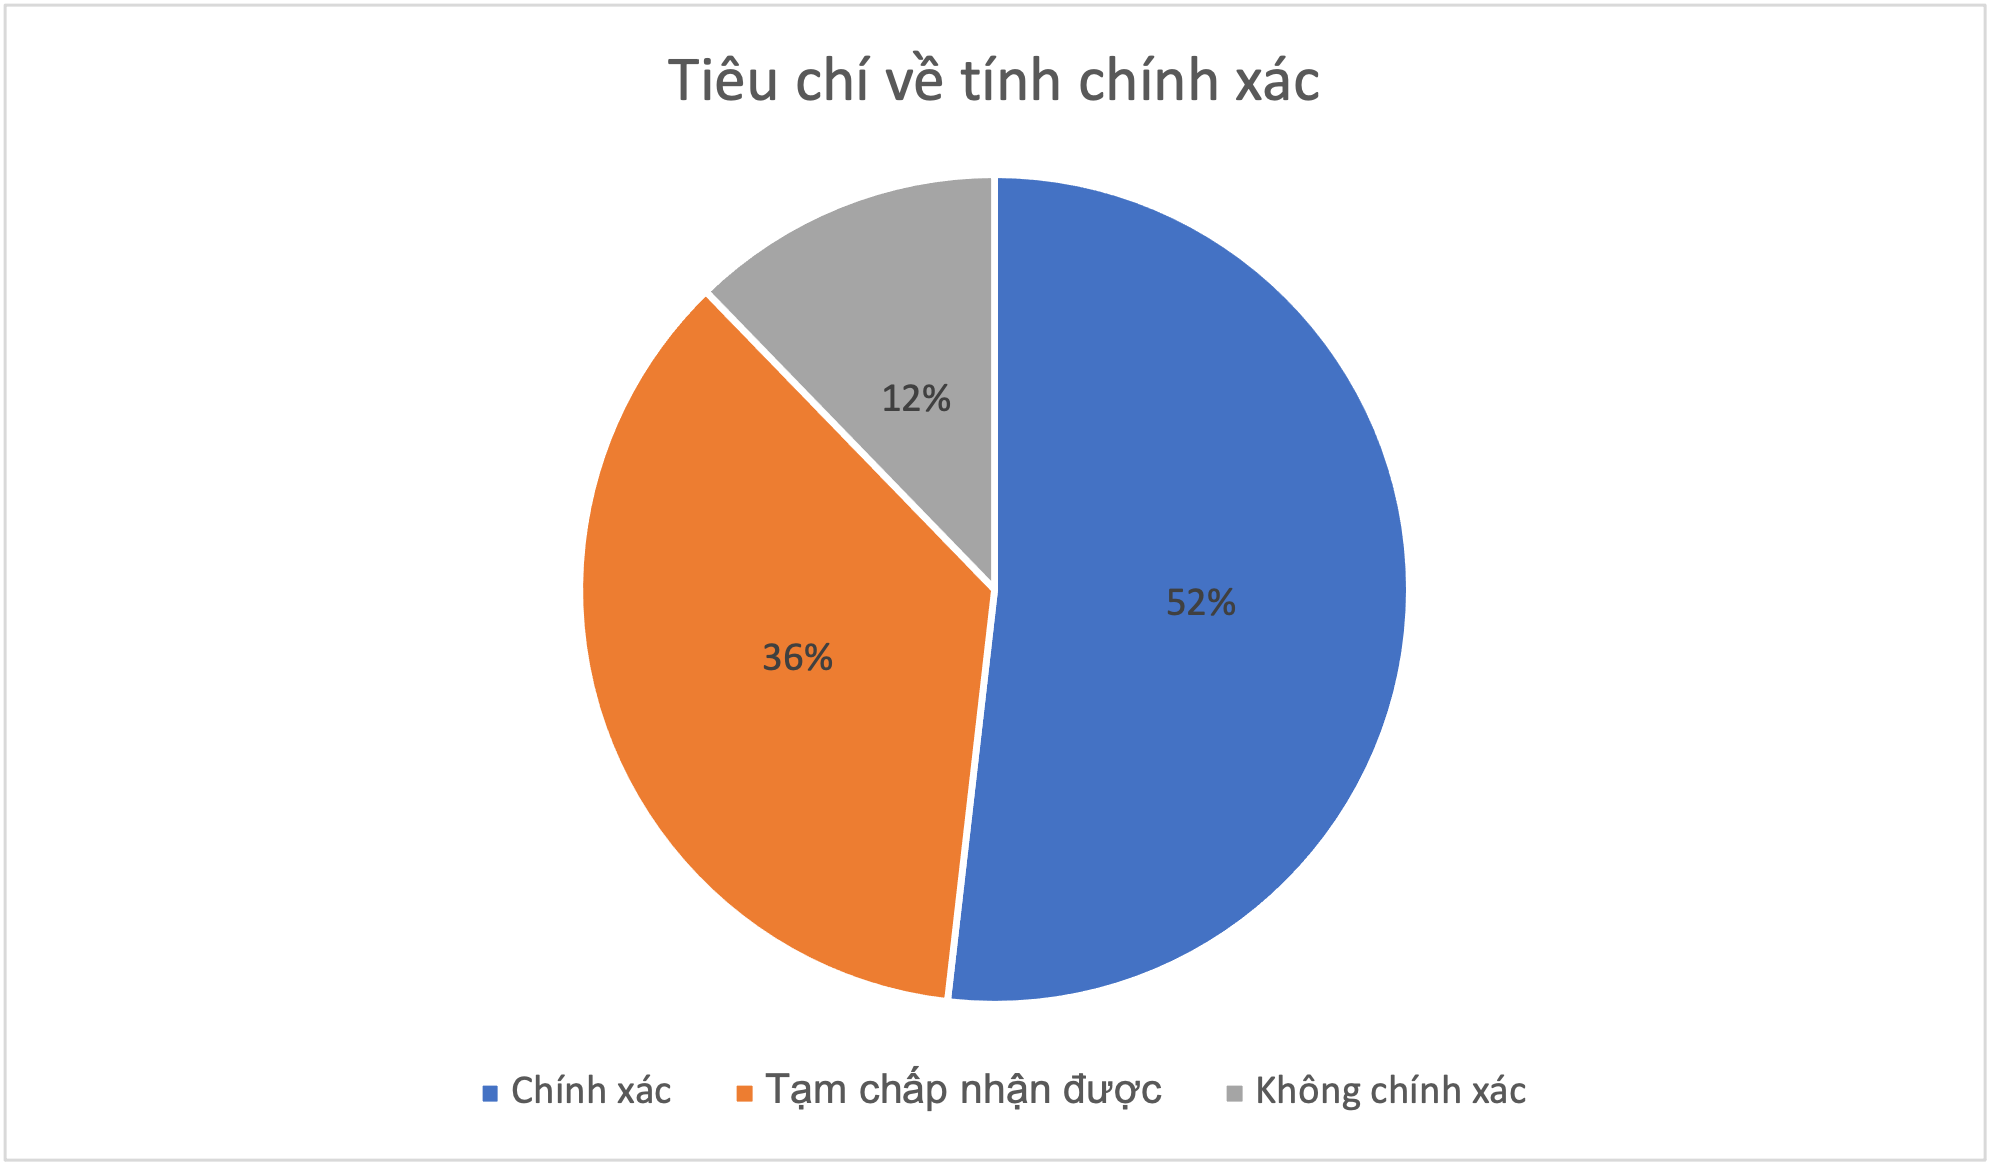
\includegraphics[scale=0.91]{thesis/chatbot/ketqua/img/tieuchi5.png}
    \caption{Kết quả đánh giá tiêu chí tính chính xác}
    \label{fig:tieuchi5}
\end{figure}

\textbf{Nhận xét:}
Có 90\% nhận xét từ tạm chấp nhận được cho đến chính xác. Trong đó
hơn 50\% là chính xác. Chỉ có 12\% nhận xét là không chính xác.
Hiện tại việc xác định thông tin người dùng thắc mắc là đúng hay
sai chỉ thực hiện thông qua phương pháp so trùng đơn giản nên việc
xác định này cũng còn khá hạn chế.

\subsubsection{Tiêu chí về mức độ đáp ứng nhu cầu tư vấn sản phẩm
nói chung}
Hình \ref{fig:tieuchi6} mô tả kết quả đánh giá của người dùng cho
tiêu chí về mức độ đáp ứng nhu cầu tư vấn sản phẩm nói chung.

\begin{figure}[ht!]
    \centering
    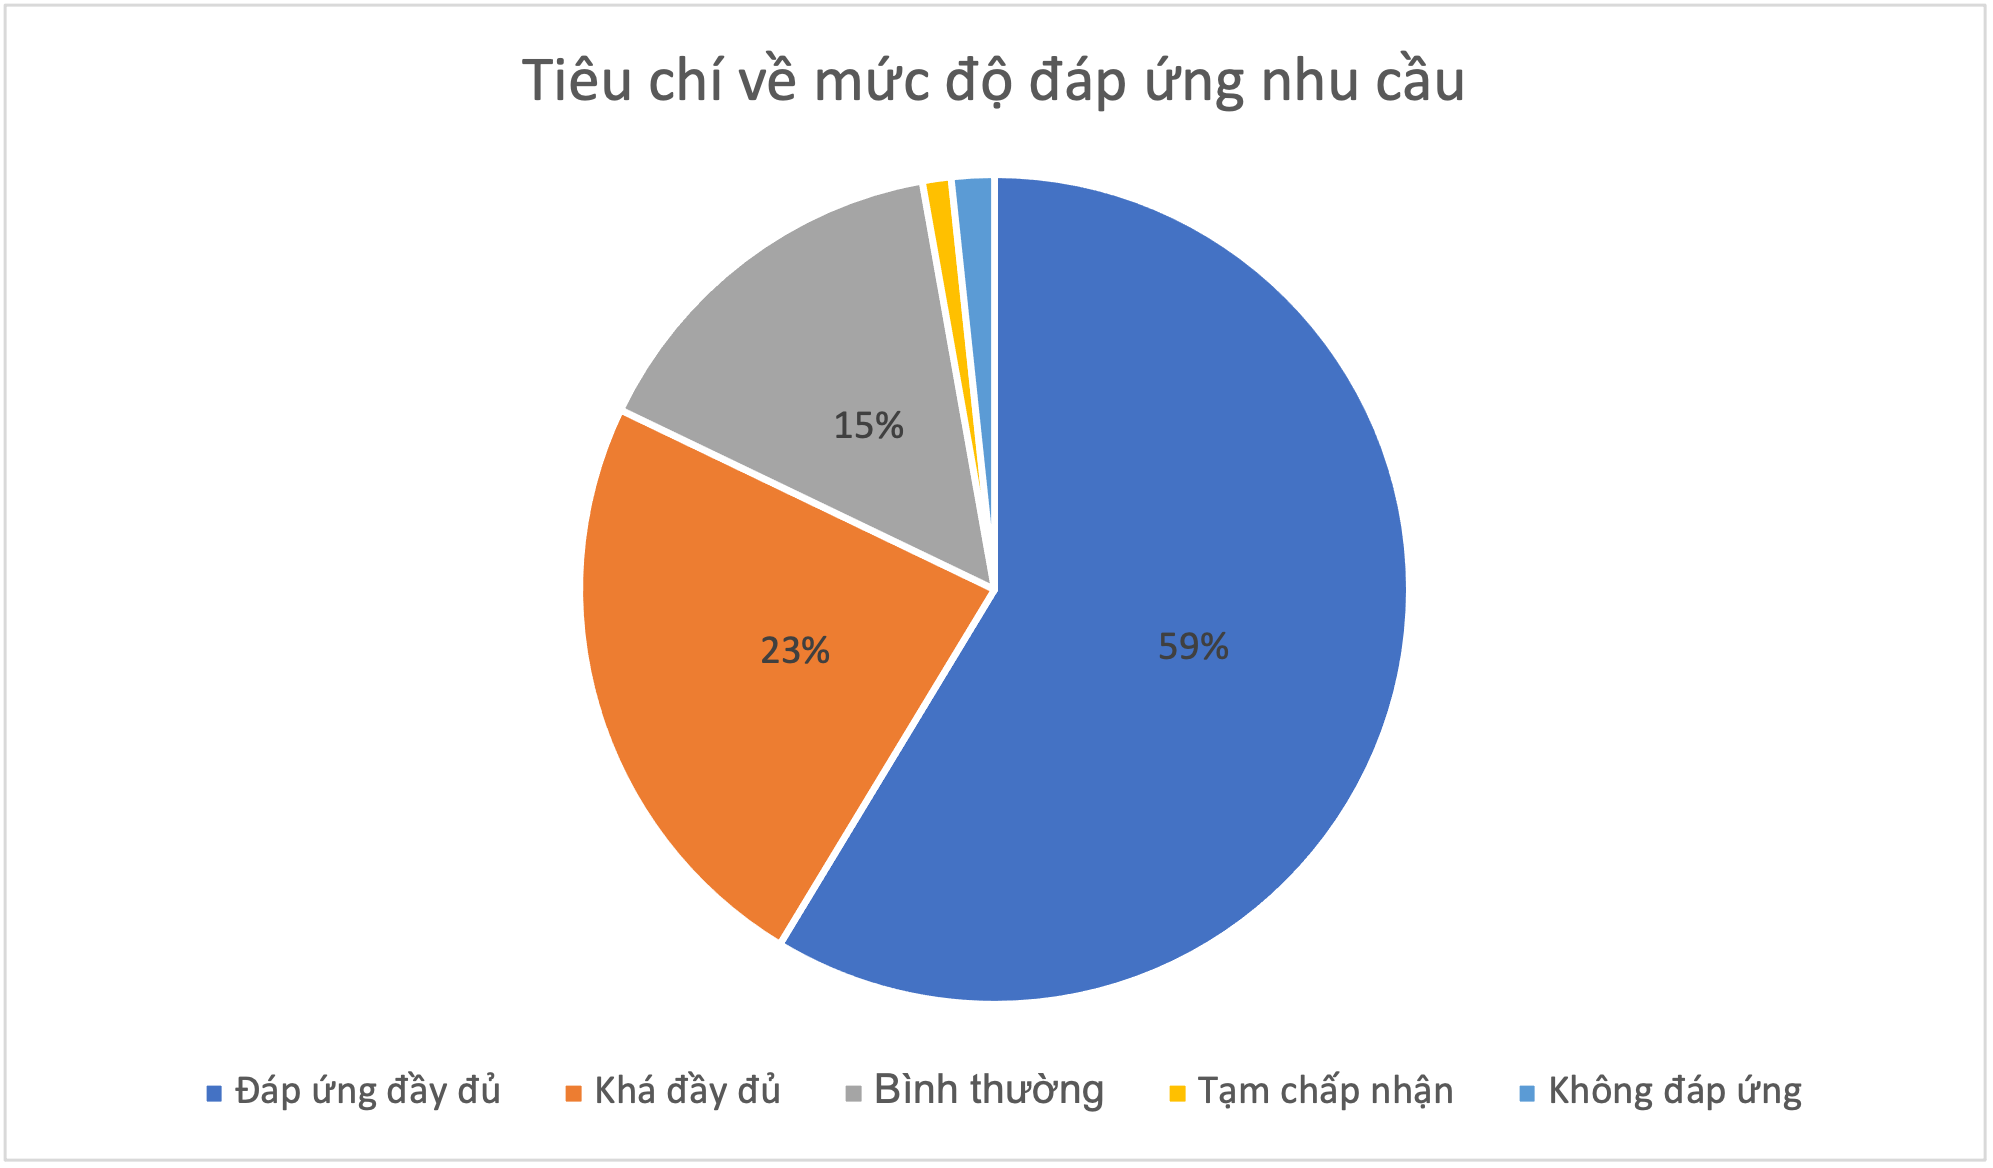
\includegraphics[scale=0.91]{thesis/chatbot/ketqua/img/tieuchi6.png}
    \caption{Kết quả đánh giá tiêu chí mức độ đáp ứng nhu cầu}
    \label{fig:tieuchi6}
\end{figure}

\begin{figure}[ht!]
    \centering
    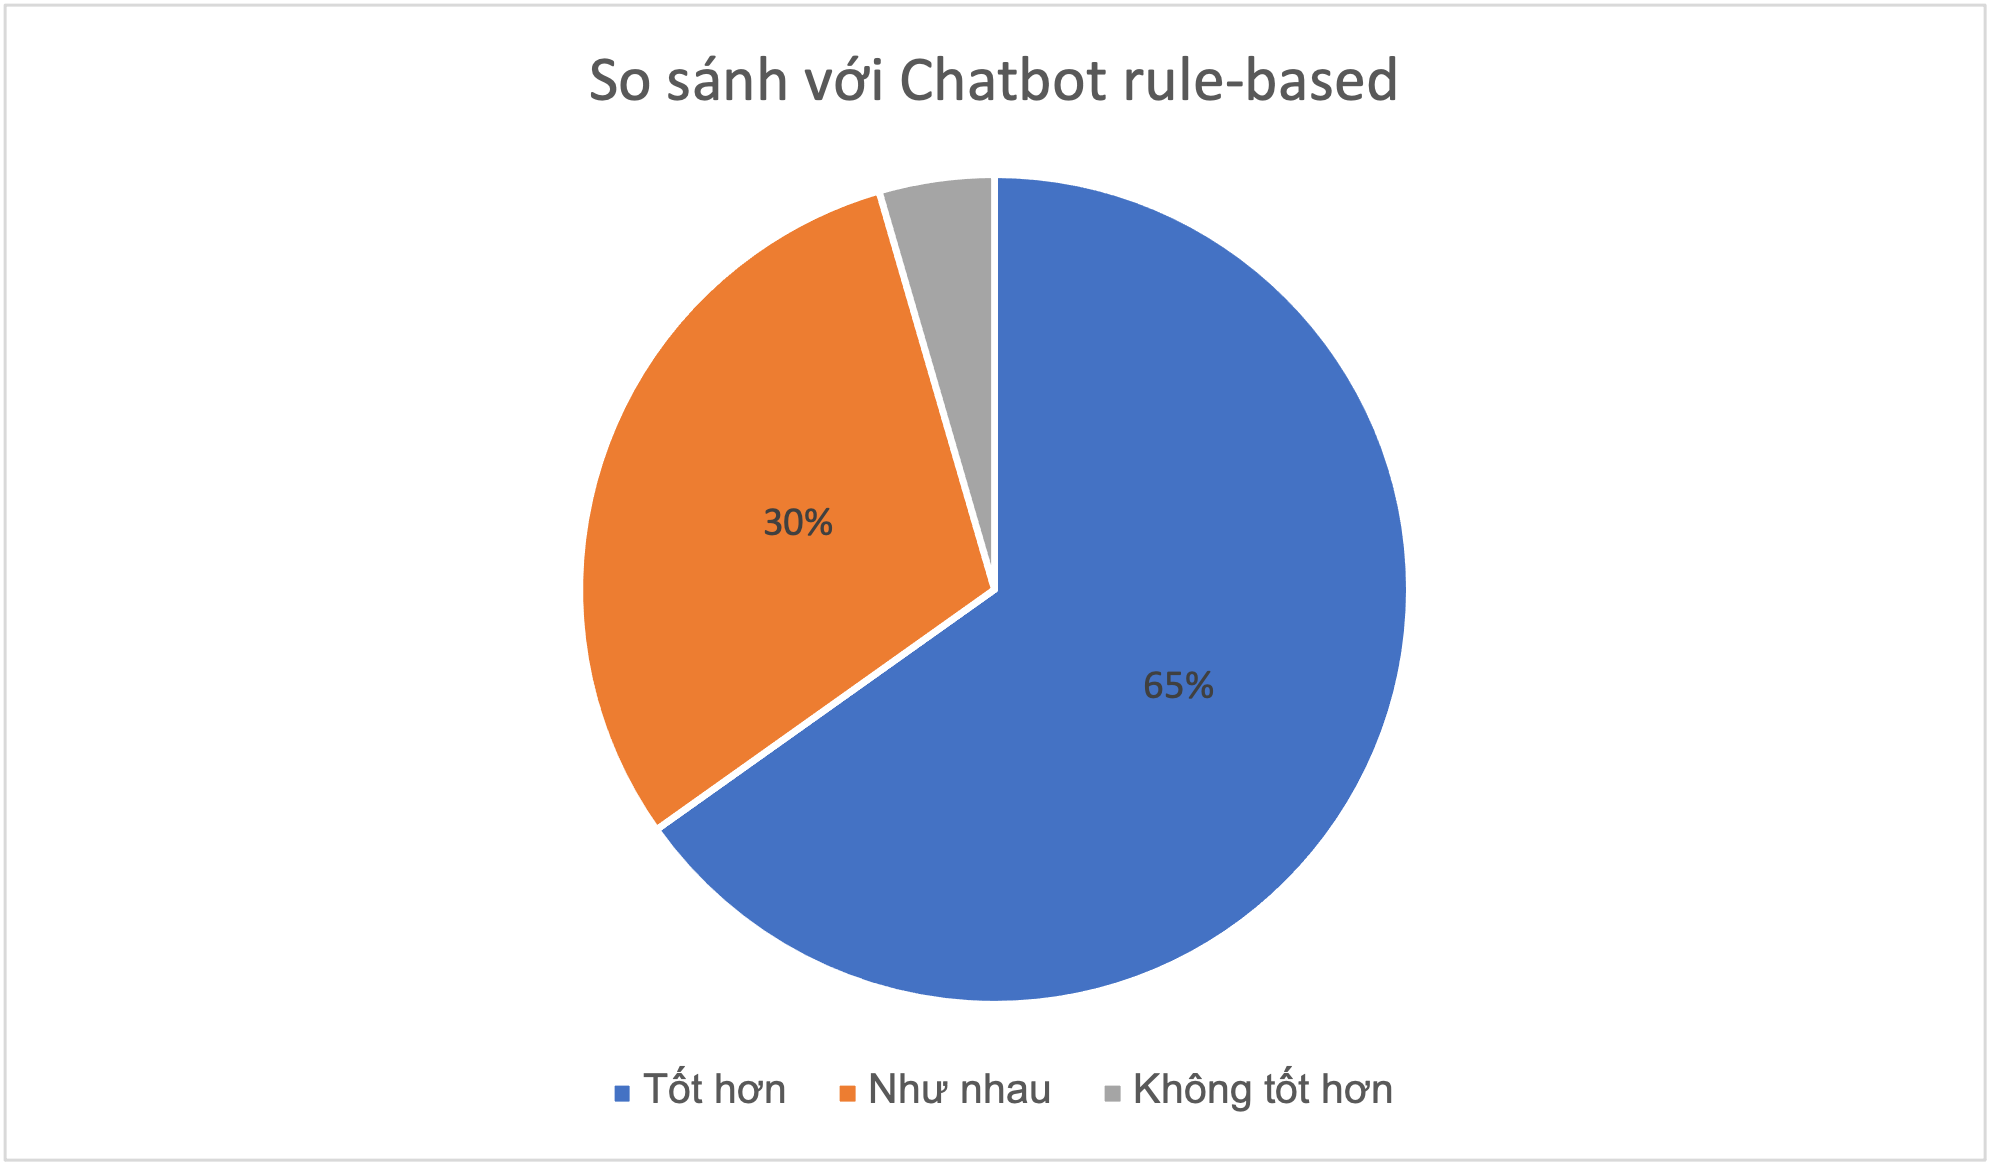
\includegraphics[scale=0.91]{thesis/chatbot/ketqua/img/tieuchi6_2.png}
    \caption{Kết quả so sánh với Chatbot rule-based}
    \label{fig:tieuchi62}
\end{figure}

\textbf{Nhận xét:}
Có 97\% nhận xét từ bình thường cho đến đáp ứng đầy đủ. Trong đó hơn
50\% là đáp ứng đầy đủ. Kết quả đánh giá như vậy là rất cao. Biểu thị
Chatbot được huấn luyện đáp ứng rất tốt các yêu cầu của người dùng.
Tuy nhiên, ta vẫn có 2\% nhận xét là không đáp ứng. Như đã đề cập về
những hạn chế ở những mục trước cũng như vấn đề về dữ liệu thực tế
chưa thực sự đầy đủ dẫn đến việc thông tin người dùng cần vẫn
chưa được cung cấp đầy đủ và chính xác.

\subsubsection{So sánh với Chatbot rule-based}
Hình \ref{fig:tieuchi62} mô tả kết quả đánh giá của người dùng khi
so sánh tiêu chí mức độ đáp ứng nhu cầu với Chatbot rule-based.

\textbf{Nhận xét:}
Có 95\% đánh giá là tốt hơn hoặc tương đương với Chatbot rule-based.
Chỉ có 5\% là không tốt hơn. Tương tự với nguyên nhân được đề cập ở
các tiêu chí trước, Chatbot rule-based này sẽ liệt kê tất cả thông tin
của sản phẩm trong lượt đầu. Việc này thỏa mãn một số người dùng tốt
hơn Chatbot khi sử dụng học tăng cường.

\subsubsection{Tiêu chí về mức độ giao tiếp tự nhiên trong suốt
cuộc hội thoại}
Hình \ref{fig:tieuchi7} mô tả kết quả đánh giá của người dùng cho
tiêu chí về mức độ giao tiếp tự nhiên trong suốt cuộc hội thoại.

\begin{figure}[ht!]
    \centering
    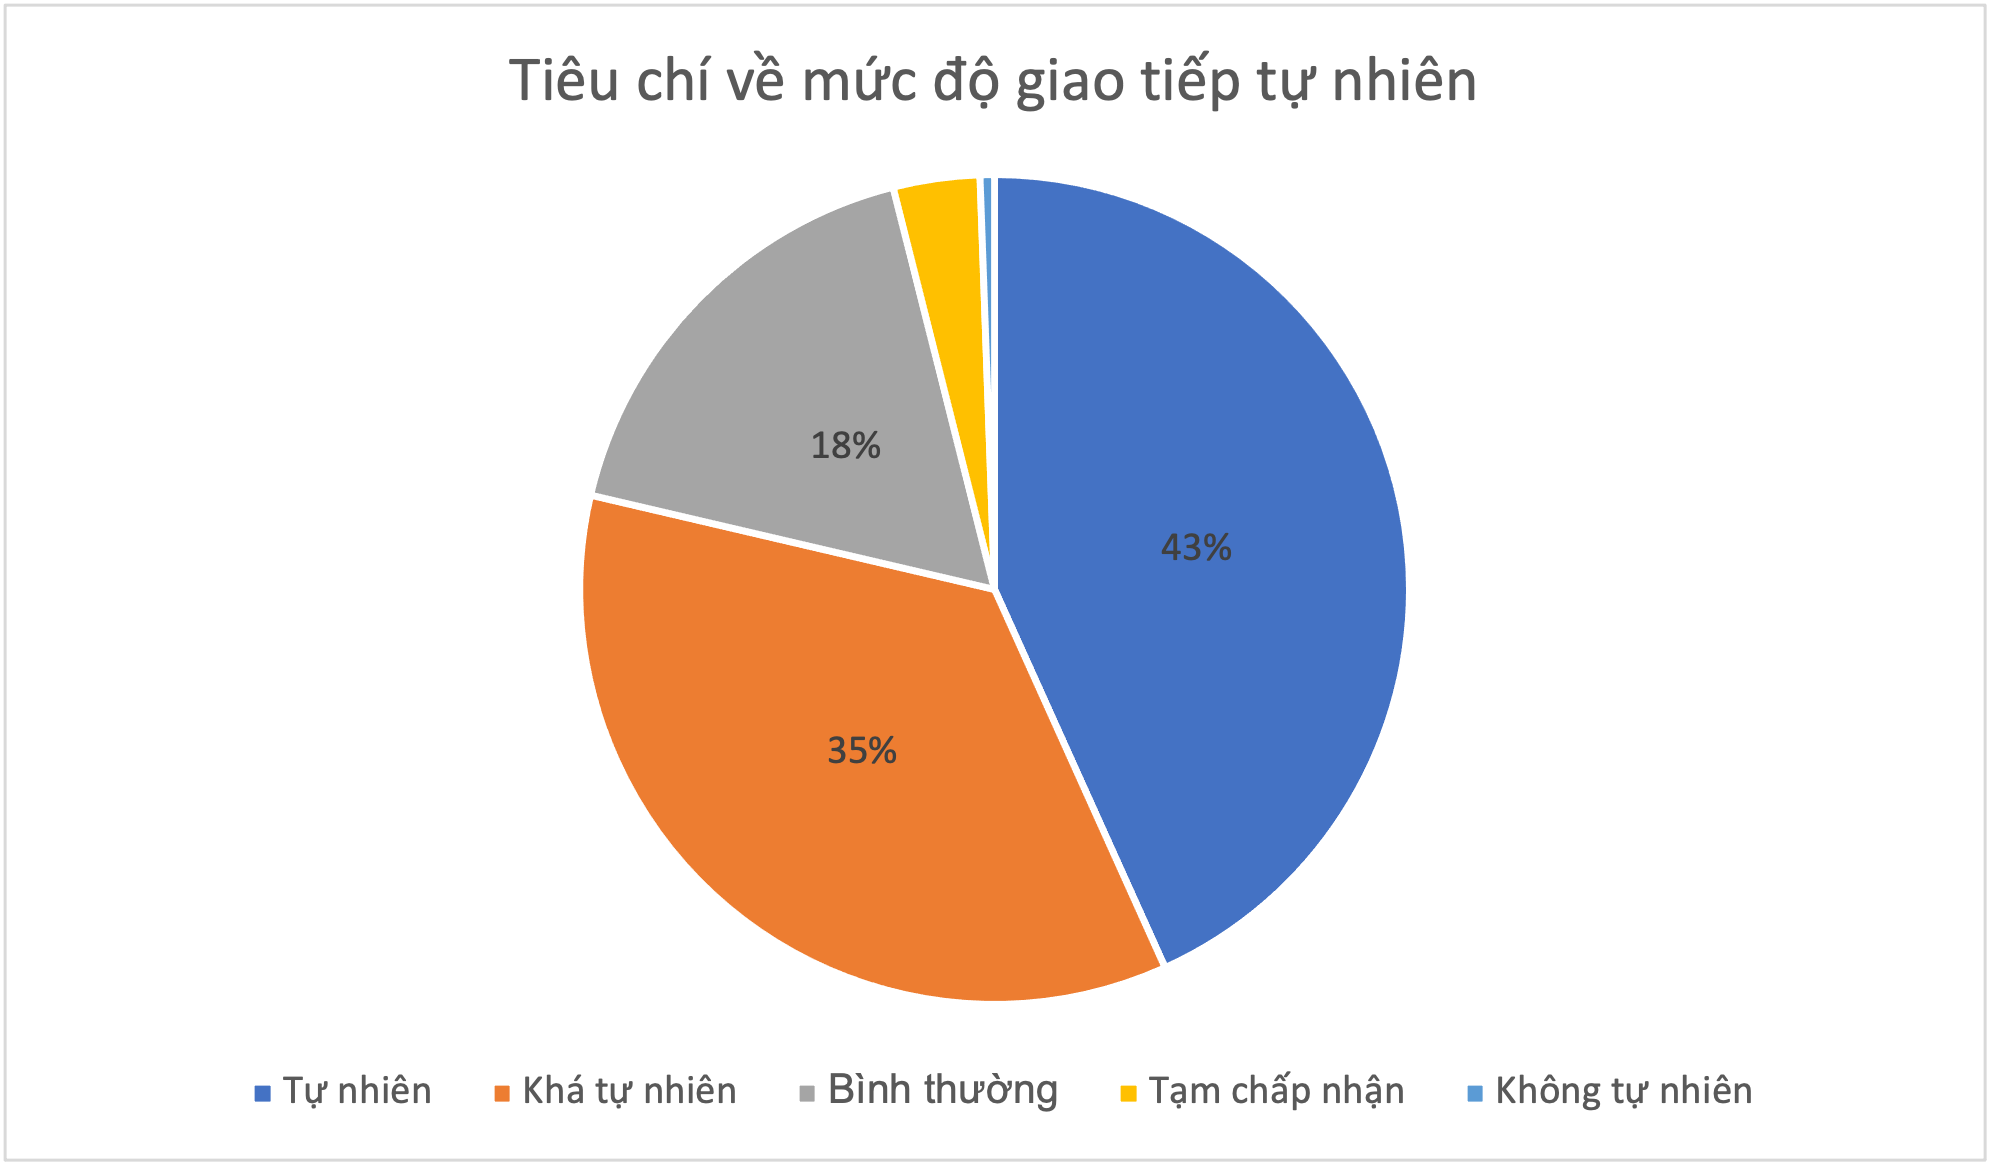
\includegraphics[scale=0.91]{thesis/chatbot/ketqua/img/tieuchi7.png}
    \caption{Kết quả đánh giá tiêu chí mức độ giao tiếp tự nhiên}
    \label{fig:tieuchi7}
\end{figure}

\textbf{Nhận xét:}
Có 96\% nhận xét từ bình thường cho đến tự nhiên. Trong đó gần 50\%
là tự nhiên. Chỉ có 1\% là không tự nhiên. Kết quả đánh giá như vậy
là rất cao. Biểu thị Chatbot được huấn luyện giao tiếp với người dùng
một cách tự nhiên phù hợp.

\subsubsection{So sánh với Chatbot rule-based}
Hình \ref{fig:tieuchi72} mô tả kết quả đánh giá của người dùng khi
so sánh tiêu chí mức độ giao tiếp tự nhiên với Chatbot rule-based.

\begin{figure}[ht!]
    \centering
    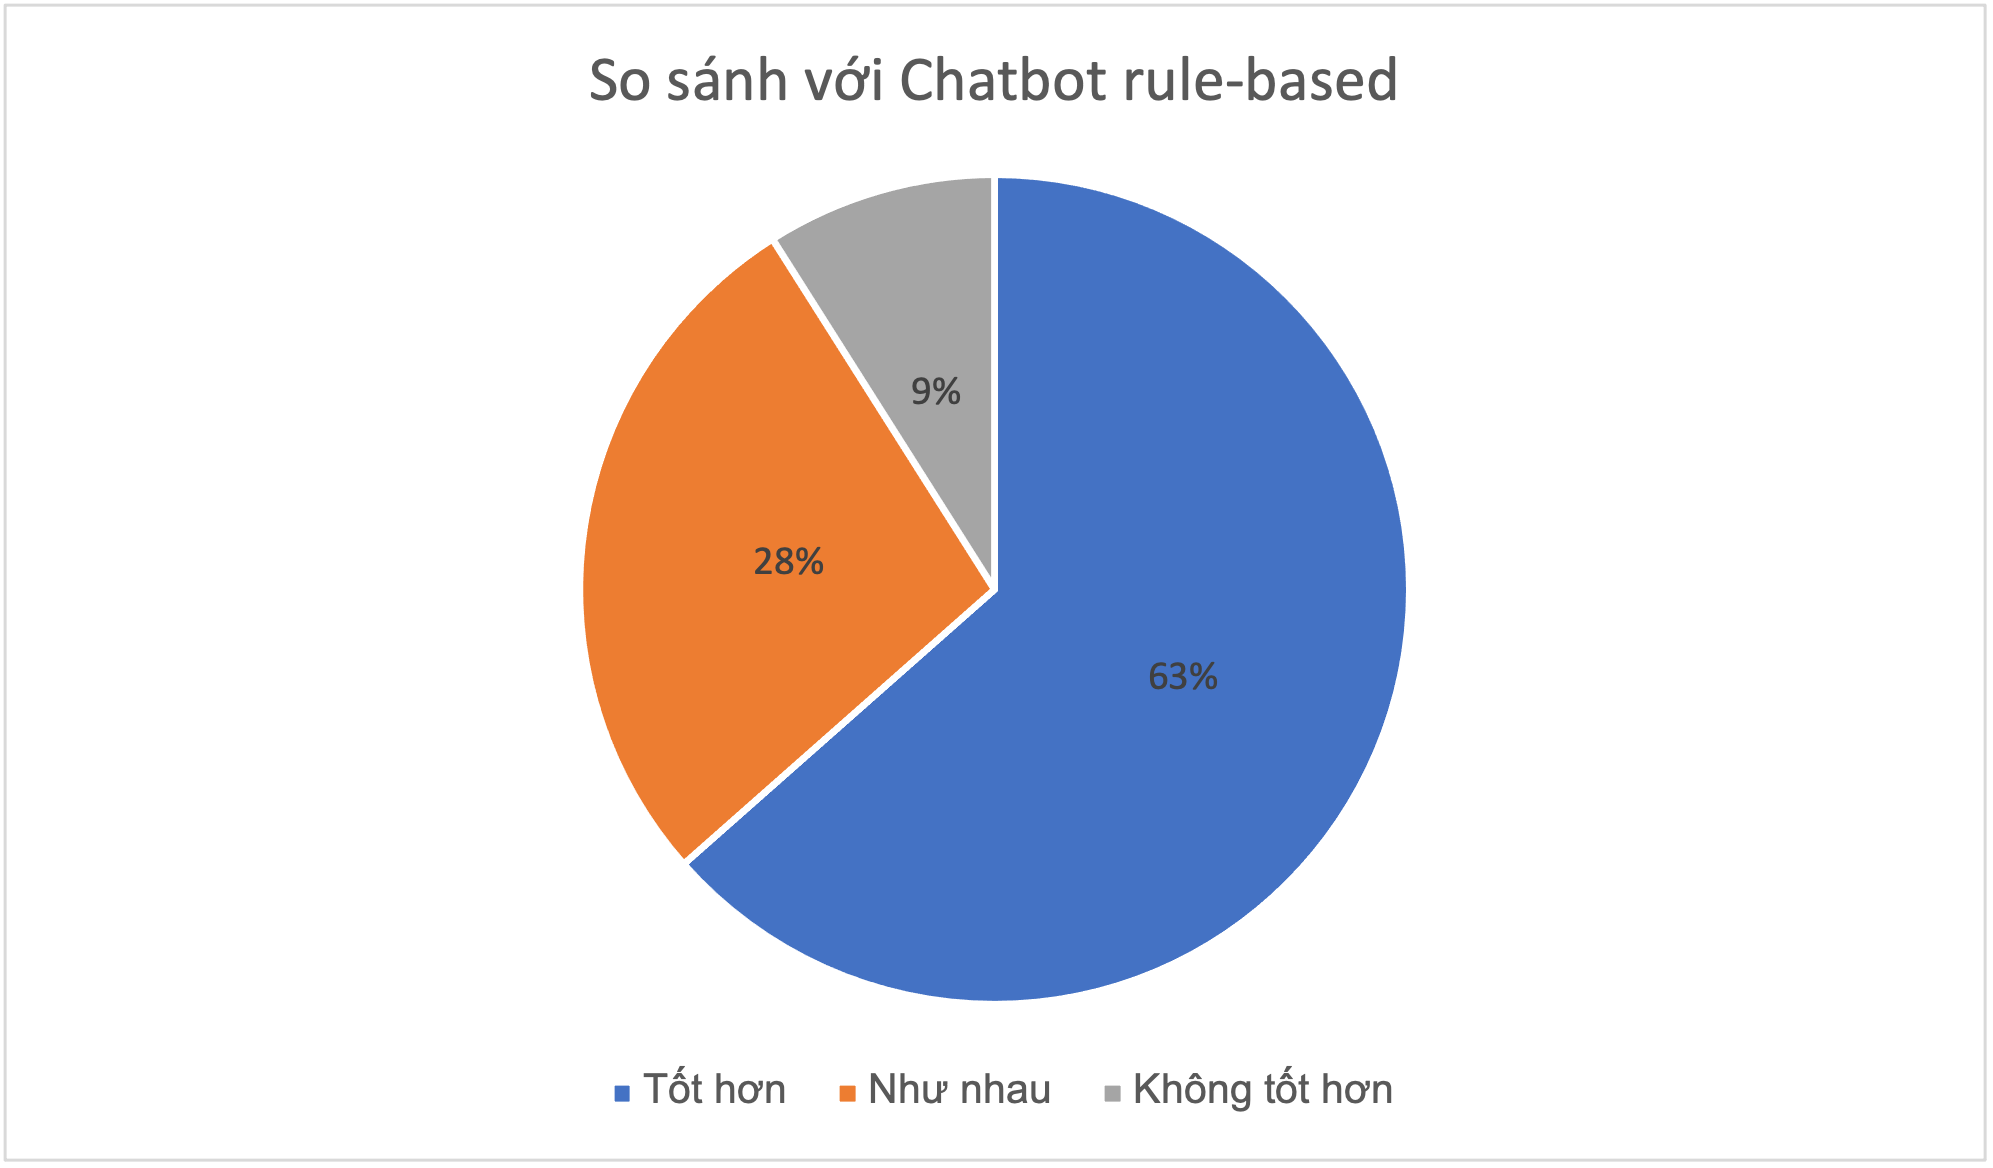
\includegraphics[scale=0.91]{thesis/chatbot/ketqua/img/tieuchi7_2.png}
    \caption{Kết quả so sánh với Chatbot rule-based}
    \label{fig:tieuchi72}
\end{figure}

\textbf{Nhận xét:}
Có hơn 90\% đánh giá là tốt hơn hoặc tương đương với Chatbot rule-based.
Chỉ có 9\% là không tốt hơn. Yếu tố tự nhiên được đánh giá tùy vào
cảm tính của người dùng. Một phần có thể do bộ sinh phản hồi
chưa được tốt.

\subsubsection{Đánh giá tổng quan của người dùng}
Hình \ref{fig:tieuchi8} mô tả kết quả đánh giá tổng quan của người dùng
trên thang đánh giá 5 sao.

\begin{figure}[ht!]
    \centering
    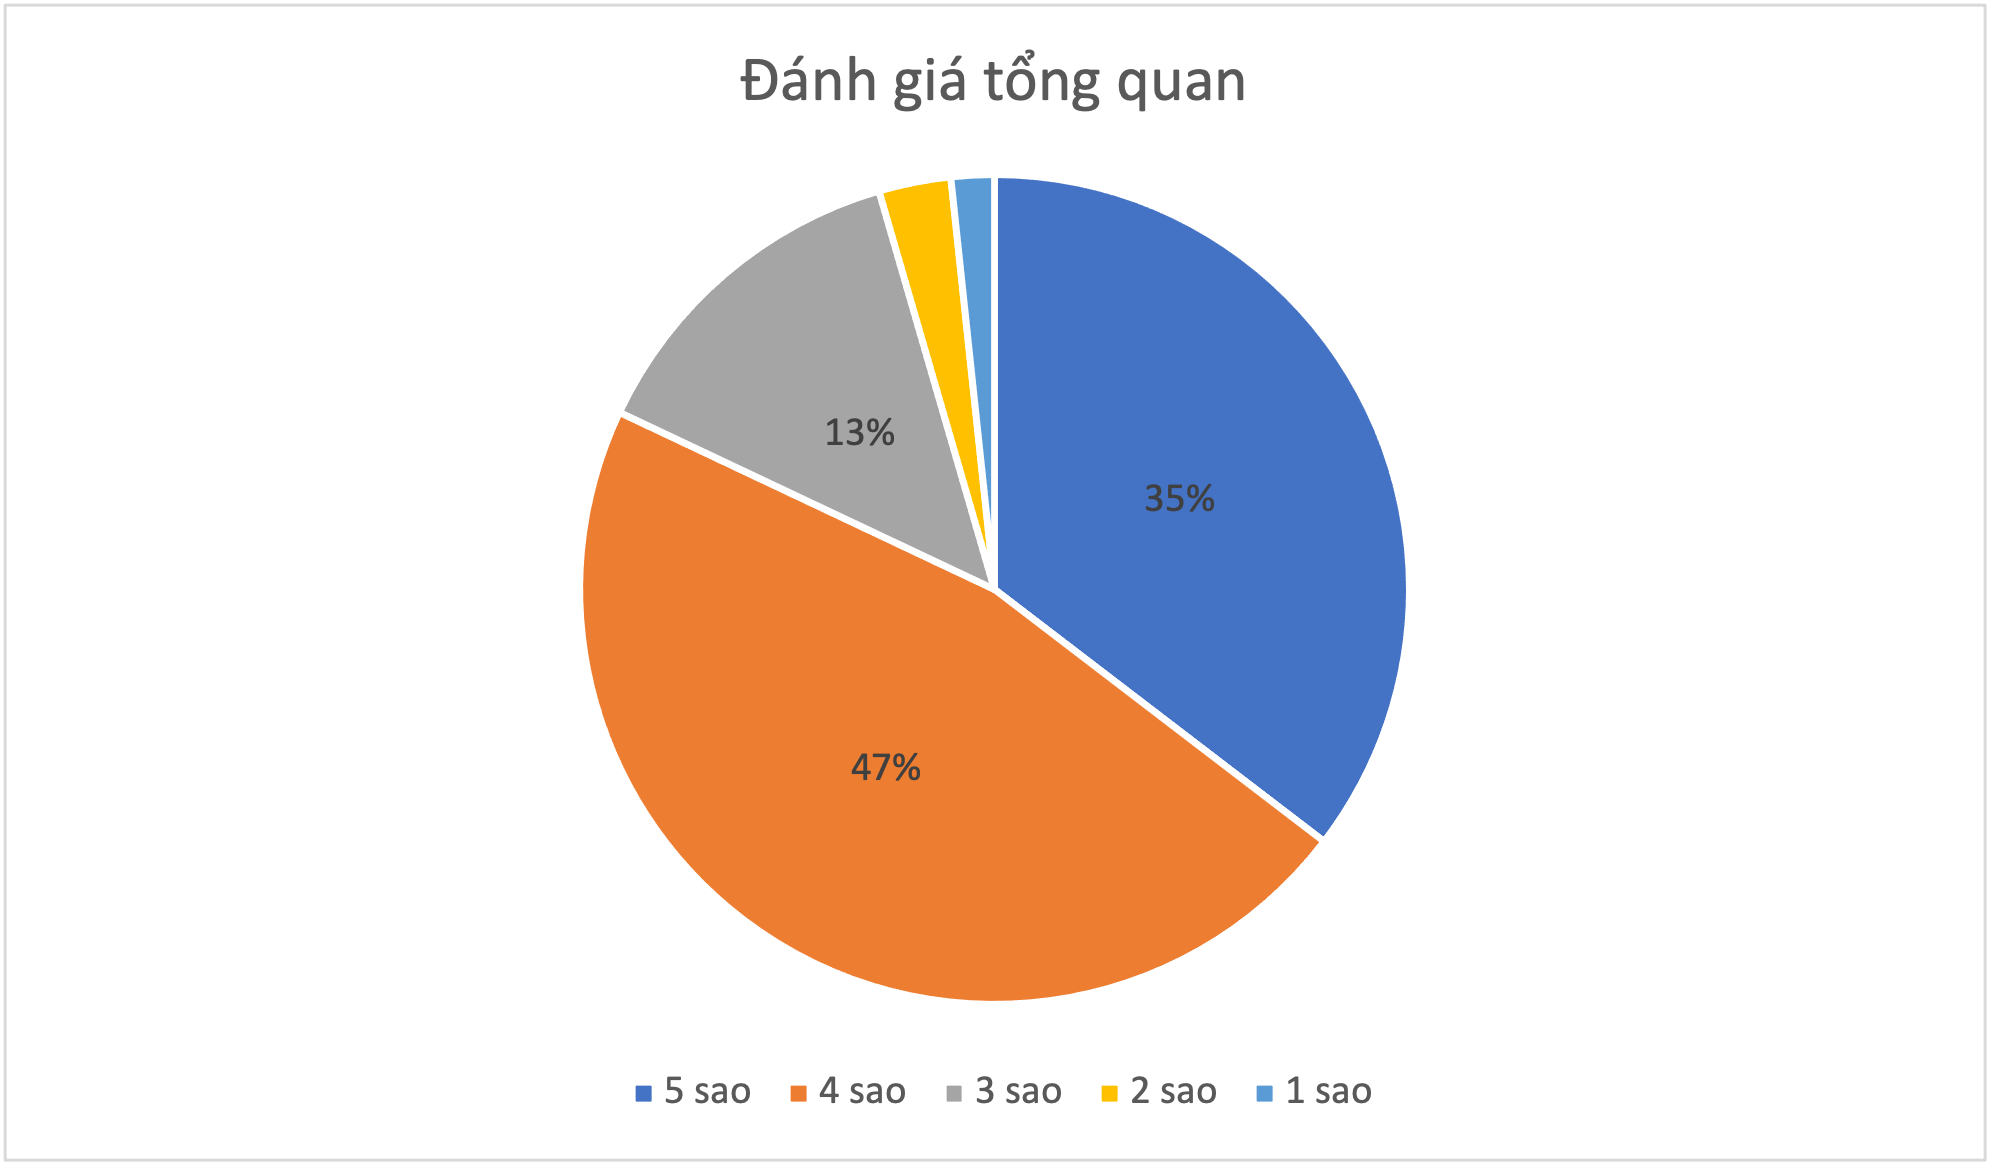
\includegraphics[scale=0.91]{thesis/chatbot/ketqua/img/tieuchi8.png}
    \caption{Kết quả đánh giá tổng quan của người dùng}
    \label{fig:tieuchi8}
\end{figure}

\textbf{Nhận xét:}
Kết quả cho thấy có 95\% người dùng đánh giá từ 3 sao trở lên.
Xét trên thang điểm 5 sao, Chatbot đạt 4.1 sao.

\section{Kiểm thử ứng dụng Chatbot}
Kiểm thử hệ thống thuộc loại kiểm thử hộp đen (black box). Kiểm thử
hệ thống là kiểm tra được thực hiện trên một hệ thống tích hợp
hoàn chỉnh để đánh giá sự tuân thủ của hệ thống với các yêu cầu đã
chỉ định của nó. Nội dung kiểm thử và tiêu chí đánh giá được
mô tả cụ thể sau đây.

\subsection{Kiểm thử giao diện}
Nội dung kiểm thử được mô tả cụ thể ở bảng \ref{tab:uitest}.

\begin{table}[!ht]
\caption{Đặc tả kiểm thử giao diện Chatbot}
\label{tab:uitest}
\centering
\begin{tabular}{|C{0.8cm}|L{3.2cm}|L{3.2cm}|L{3.6cm}|C{1.8cm}|}
\hline
\textbf{STT} &
\centering\textbf{Chức năng} &
\centering\textbf{Nội dung kiểm thử} &
\centering\textbf{Kết quả mong đợi} &
\textbf{Kết quả kiểm thử} \\ % inserts table %heading
\hline
1 &
Giao diện Chatbot với các nút bấm chức năng, ô lựa chọn, khung
hội thoại và toàn bộ tin nhắn của người dùng và tác nhân cho tới
thời điểm hiện tại &
Bước 1: Truy cập vào ứng dụng Chatbot.
Bước 2: Thực hiện thao tác trên các nút bấm chức năng. &
Giao diện Chatbot hiển thị đầy đủ các nút bấm, ô lựa chọn, khung
hội thoại và toàn bộ tin nhắn của người dùng và tác nhân cho tới
thời điểm hiện tại, Kết quả minh họa như hình \ref{fig:testtool} &
PASS \\
\hline
2 &
Giao diện Chatbot với kích thước trên các thiết bị có độ
phân giải và kích thước khác nhau &
Bước 1: Truy cập vào ứng dụng Chatbot với các
trình duyệt khác nhau.
Bước 2: Thu nhỏ hoặc phóng lớn cửa sổ. &
Giao diện Chatbot giữ nguyên kích thước trên các thiết bị có độ
phân giải và kích thước khác nhau, không bị khuất, bị mất nội dung &
PASS \\
\hline
3 &
Các hiệu ứng hành động trên giao diện Chatbot &
Bước 1: Truy cập vào ứng dụng Chatbot.
Bước 2: Thực hiện thao tác trên ứng dụng, quan sát các thay đổi
trên giao diện. &
Các hiệu ứng hành động trên giao diện Chatbot hiển thị mượt mà,
không gặp hiện tượng giật, đứng khi sử dụng &
PASS \\
\hline
\end{tabular}
\end{table}

\begin{figure}[ht!]
    \centering
    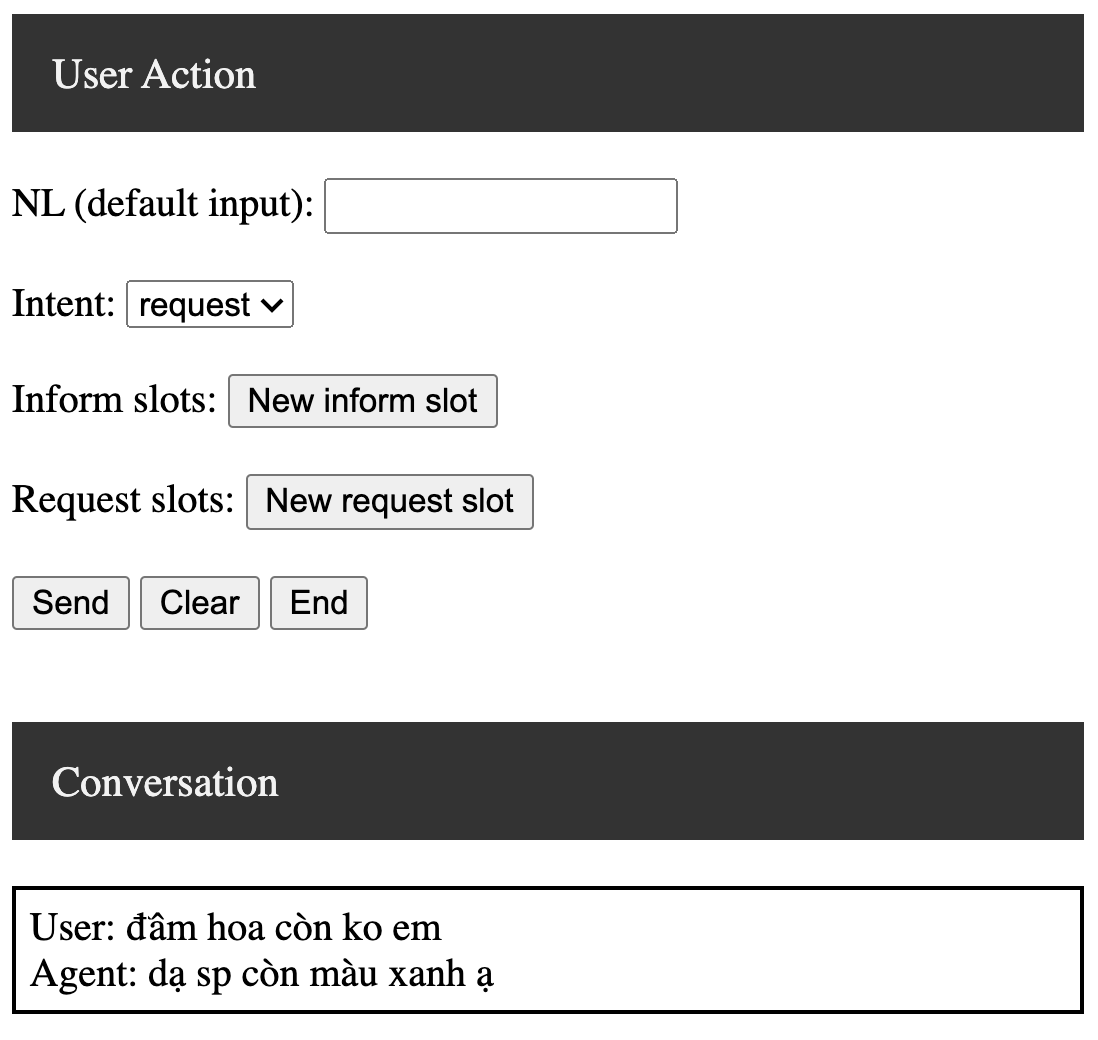
\includegraphics[scale=0.6]{thesis/chatbot/ketqua/img/test_tool.png}
    \caption{Giao diện của Chatbot}
    \label{fig:testtool}
\end{figure}

\subsection{Kiểm thử chức năng}
Nội dung kiểm thử được mô tả cụ thể ở bảng \ref{tab:functiontest}.

\begin{table}[!ht]
\caption{Đặc tả kiểm thử chức năng Chatbot}
\centering
\begin{tabular}{|C{0.8cm}|L{2cm}|L{4.4cm}|L{3.6cm}|C{1.8cm}|}
\hline
\textbf{STT} &
\centering\textbf{Chức năng} &
\centering\textbf{Nội dung kiểm thử} &
\centering\textbf{Kết quả mong đợi} &
\textbf{Kết quả kiểm thử} \\ % inserts table %heading
\hline
1 &
Gửi hành động người dùng &
Bước 1: Nhập câu thoại hoặc lựa chọn hành động thông qua các ô lựa chọn.
Bước 2: Gửi hành động. &
Chatbot nhận được hành động của người dùng, không sai lệch, thiếu thông tin &
PASS \\
\hline
2 &
Xóa hành động người dùng &
Bước 1: Nhập câu thoại hoặc lựa chọn hành động thông qua các ô lựa chọn.
Bước 2: Xóa hành động. &
Chatbot xóa hành động đang nhập hiện tại của người dùng.
Trạng thái hội thoại không thay đổi &
PASS \\
\hline
3 &
Phản hồi người dùng &
Bước 1: Nhập câu thoại hoặc lựa chọn hành động thông qua các ô lựa chọn.
Bước 2: Gửi hành động. &
Chatbot có phản hồi với mỗi tin nhắn của người dùng và hiển thị câu
phản hồi trên khung hội thoại &
PASS \\
\hline
4 &
Kết thúc hội thoại &
Bước 1: Nhập câu thoại hoặc lựa chọn hành động thông qua các ô lựa chọn.
Bước 2: Gửi hành động.
Bước 3: Nhấn nút kết thúc hội thoại. &
Chatbot xóa toàn bộ nội dung hội thoại, đồng thời thiết lập lại
trạng thái hội thoại &
PASS \\
\hline
\end{tabular}
\label{tab:functiontest}
\end{table}

% \subsection{Kiểm thử đơn vị}

% \subsubsection{Bộ truy vấn cơ sở dữ liệu}

% \subsubsection{Bộ xử lý phản hồi người dùng}

% \subsubsection{Bộ quản lý trạng thái hội thoại}

% \subsubsection{Bộ sinh phản hồi}

% \subsubsection{Bộ sinh câu phản hồi}

\chapter{Tổng kết}

Trong chương này, tổng kết những kết quả đạt được trong Luận văn này,
một số mặt hạn chế của đề tài và hướng phát triển trong tương lai.

\section{Các kết quả đạt được}
Những công việc đã đạt được:

\begin{itemize}
    \item Tìm kiếm và thu thập dữ liệu phù hợp với nội dung đề tài.
    \item Tổ chức đánh nhãn với sự giúp đỡ của các bạn cộng tác viên.
    \item Khảo sát nhu cầu của người dùng và cửa hàng cụ thể trong
    tư vấn thông tin sản phẩm, từ đó xây dựng các kịch bản, nhiệm vụ
    cho Chatbot.
    \item Tiến hành huấn luyện mô hình học tăng cường để có thể đưa ra
    quyết định cho mỗi hành động khi giao tiếp với người dùng cũng như
    truy vấn dữ liệu chính xác để trả về đúng thông tin người dùng mong muốn.
    \item Xây dựng bộ sinh câu phản hồi của Chatbot với ngôn từ
    tự nhiên tạo cảm giác thoải mái cho người dùng.
    \item Tổ chức đánh giá chất lượng hệ thống và thu được phản hồi
    tích cực từ người dùng.
\end{itemize}

\section{Các hạn chế}
Một số hạn chế của hệ thống:

\begin{itemize}
    \item Quá trình chuẩn hóa dữ liệu còn nhiều thiếu sót, việc này
    phụ thuộc vào bộ từ điển dữ liệu. Từ đó, phát sinh các trường hợp
    không nhận diện được đúng đắn thông tin người dùng cung cấp.
    \item Mỗi một cuộc hội thoại diễn ra, mô hình này chỉ tư vấn và
    chốt được đơn hàng cho một loại sản phẩm. Việc này dễ thấy thông qua
    định dạng hành động của người dùng lẫn tác nhân. Các thông tin
    phụ thuộc lẫn nhau như tên sản phẩm đi kèm với kích cỡ hay
    màu sắc, ... không có cấu trúc phân cấp.
\end{itemize}

\section{Định hướng trong tương lai}
Một số cải tiến cho hệ thống này như sau:

\begin{itemize}
    \item Cập nhật thêm các ý định của người dùng để quá trình tư vấn
    phong phú, hỗ trợ tốt hơn cho người dùng.
    \item Tìm cách sử dụng các mô hình học máy hoặc phương án khác
    hỗ trợ cho việc chuẩn hóa tốt hơn.
    \item Tìm cách sửa đổi định dạng hành động cũng như bộ quản lý
    trạng thái hội thoại, cách thức quản lý thông tin được thông báo
    hoặc yêu cầu tương ứng với nhau.
    \item Mô hình tư vấn này có thể được tích hợp trong nhiều hệ thống
    Chatbot khác.
\end{itemize}


\begin{thebibliography}{99}
\raggedright
% reference in chapter 2
\bibitem{automatedmedical}
K. Rarhi \textit{et al.}, (2017, Jan). \enquote{Automated Medical Chatbot}.
\textit{SSRN Electronic Journal}. [Online].
Available: \url{https://ssrn.com/abstract=3090881}

\bibitem{superagent}
L. Cui \textit{et al.},
\enquote{SuperAgent: A Customer Service Chatbot for E-commerce Websites},
in \textit{ACL 2017, System Demonstrations}, 2017, pp. 97–102.

\bibitem{airport}
M. Carisi \textit{et al.}, \enquote{Design and implementation of an airport chatbot},
in \textit{The 5th EAI International Conference on Smart Objects and Technologies for Social Good}, 2019, pp. 49–54.

\bibitem{commerce}
S. Angelov, and M. Lazarova, \enquote{E-commerce Distributed Chatbot System},
in \textit{The 9th Balkan Conference on Informatics}, 2019, pp. 1-8.

\bibitem{clustered}
H. Cuayáhuitl \textit{et al.}, \enquote{Deep Reinforcement Learning for Chatbots
Using Clustered Actions and Human-Likeness Rewards},
presented at International Joint Conference of Neural Networks, 2019.

\bibitem{generation}
J. Li \textit{et al.}, \enquote{Deep Reinforcement Learning for Dialogue Generation},
in \textit{The 2016 Conference on Empirical Methods in Natural Language Processing}, 2016, pp. 1192–1202.

\bibitem{gradient}
R. J. Williams, \enquote{Simple statistical gradient following algorithms for connectionist reinforcement learning},
in \textit{Machine Learning}, vol. 8, Hendrik Blockeel, 1992, pp. 229–256.

\bibitem{selfimproving}
E. Ricciardelli and D. Biswas, \enquote{Self-improving Chatbots based on Reinforcement Learning},
presented at 4th Multidisciplinary Conference on Reinforcement Learning and Decision Making, Montreal, Canada, 2019.

\bibitem{traininggochatbot}
M. Brenner, \enquote{Training a Goal-Oriented Chatbot with Deep Reinforcement Learning}.
Internet: \url{https://towardsdatascience.com/training-a-goal-oriented-chatbot-with-deep-reinforcement-learning-part-i-introduction-and-dce3af21d383}, Dec. 2, 2018.

\bibitem{endtoend}
Xiujun Li \textit{et al.}, \enquote{End-to-End Task-Completion Neural Dialogue Systems},
in \textit{The 8th International Joint Conference on Natural Language Processing}, Taipei, Taiwan, 2017, pp. 733–743.

% reference in chapter 3
\bibitem{reinforcementlearninganintroduction}
R. S. Sutton and A. G. Barto, \textit{Reinforcement Learning: An Introduction}.
Cambridge, MA: MIT Press, 2018.

\bibitem{introductiondeepqlearningpython}
A. Choudhary, \enquote{A Hands-On Introduction to Deep Q-Learning using OpenAI Gym in Python}.
Internet: \url{https://www.analyticsvidhya.com/blog/2019/04/introduction-deep-q-learning-python}, Apr. 18, 2019.

% reference in chapter 4
\bibitem{chatbothddoan}
Phạm Minh Hiếu, Cao Chánh Dương, \enquote{Phát triển một Chatbot thông minh để tư vấn hoạt động đoàn cho sinh viên},
Luận văn tốt nghiệp Đại học, Trường Đại học Bách Khoa TPHCM, 2020.

% reference other
\bibitem{refer1}
K. Shiruru, (2016, Sep.). \enquote{An Introduction to Artificial Neural Network}.
\textit{International Journal Of Advance Research And Innovative Ideas In Education}.
[Online]. 1(5), pp. 27-30.
Available: \url{https://www.researchgate.net/publication/319903816_AN_INTRODUCTION_TO_ARTIFICIAL_NEURAL_NETWORK}

\bibitem{refer5}
M. Mnasri, \enquote{Recent advances in conversational NLP: Towards the standardization of Chatbot building}.
Internet: \url{https://arxiv.org/pdf/1903.09025.pdf}, Mar. 21, 2019.

\bibitem{refer7}
V. Ilievski \textit{et al.}, \enquote{Goal-Oriented Chatbot Dialog Management Bootstrapping with Transfer Learning},
in \textit{The 27th International Joint Conference on Artificial Intelligence}, 2018, pp. 4115–4121.

\bibitem{refer9}
V. Ilievski, \enquote{Building Advanced Dialogue Managers for Goal-Oriented Dialogue Systems}.
Internet: \url{https://arxiv.org/pdf/1806.00780.pdf}, Jun. 3, 2018.

\bibitem{refer10}
J. Liu \textit{et al.}, \enquote{GoChat: Goal-oriented Chatbots with Hierarchical Reinforcement Learning},
presented at the 43rd International ACM SIGIR Conference on Research and Development in Information Retrieval, 2020.

\bibitem{refer11}
A. Bodirlau \textit{et al.}, \enquote{Cross-Domain Training for Goal-Oriented Conversational Agents},
in \textit{The International Conference on Recent Advances in Natural Language Processing}, Varna, Bulgaria, 2019, pp. 142–150.

\bibitem{refer12}
A. Xu \textit{et al.}, \enquote{A New Chatbot for Customer Service on Social Media},
in \textit{The 2017 CHI Conference on Human Factors in Computing Systems}, 2017, pp. 3506–3510.

\bibitem{refer13}
I. V. Serban \textit{et al.}, \enquote{A Deep Reinforcement Learning Chatbot}.
Internet: \url{https://arxiv.org/pdf/1709.02349.pdf}, Nov. 5, 2017.

\bibitem{refer14}
T. Schaul \textit{et al.}, \enquote{Prioritized Experience Replay},
presented at International Conference on Learning Representations, 2015.

\bibitem{refer15}
J. Gao \textit{et al.}, \enquote{Neural Approaches to Conversational AI},
in \textit{The 56th Annual Meeting of the Association for Computational Linguistics: Tutorial Abstracts},
Melbourne, Australia, 2019, pp. 2–7.

\end{thebibliography}

